%%
%% This is file `sample-sigconf-authordraft.tex',
%% generated with the docstrip utility.
%%
%% The original source files were:
%%
%% samples.dtx  (with options: `all,proceedings,bibtex,authordraft')
%% 
%% IMPORTANT NOTICE:
%% 
%% For the copyright see the source file.
%% 
%% Any modified versions of this file must be renamed
%% with new filenames distinct from sample-sigconf-authordraft.tex.
%% 
%% For distribution of the original source see the terms
%% for copying and modification in the file samples.dtx.
%% 
%% This generated file may be distributed as long as the
%% original source files, as listed above, are part of the
%% same distribution. (The sources need not necessarily be
%% in the same archive or directory.)
%%
%%
%% Commands for TeXCount
%TC:macro \cite [option:text,text]
%TC:macro \citep [option:text,text]
%TC:macro \citet [option:text,text]
%TC:envir table 0 1
%TC:envir table* 0 1
%TC:envir tabular [ignore] word
%TC:envir displaymath 0 word
%TC:envir math 0 word
%TC:envir comment 0 0
%%
%% The first command in your LaTeX source must be the \documentclass
%% command.
%%
%% For submission and review of your manuscript please change the
%% command to \documentclass[manuscript, screen, review]{acmart}.
%%
%% When submitting camera ready or to TAPS, please change the command
%% to \documentclass[sigconf]{acmart} or whichever template is required
%% for your publication.
%%
%%
%\documentclass[acmsmall]{acmart}
\documentclass[acmtog,review,anonymous]{acmart}
\usepackage{mathtools}
\usepackage{xspace} 
\usepackage{multirow}
\usepackage{algorithm}
\usepackage{algorithmic}
%%
%% \BibTeX command to typeset BibTeX logo in the docs
\AtBeginDocument{%
  \providecommand\BibTeX{{%
    Bib\TeX}}}

%% Rights management information.  This information is sent to you
%% when you complete the rights form.  These commands have SAMPLE
%% values in them; it is your responsibility as an author to replace
%% the commands and values with those provided to you when you
%% complete the rights form.
\setcopyright{acmlicensed}
\copyrightyear{2026}
\acmYear{2026}
\acmJournal{TOG}

%% These commands are for a PROCEEDINGS abstract or paper.
% \acmConference[Conference acronym 'XX]{Make sure to enter the correct
%   conference title from your rights confirmation email}{June 03--05,
%   2025}{Woodstock, NY}
%%
%%  Uncomment \acmBooktitle if the title of the proceedings is different
%%  from ``Proceedings of ...''!
%%
%%\acmBooktitle{Woodstock '18: ACM Symposium on Neural Gaze Detection,
%%  June 03--05, 2018, Woodstock, NY}
%\acmISBN{978-1-4503-XXXX-X/2025/06}


%%
%% Submission ID.
%% Use this when submitting an article to a sponsored event. You'll
%% receive a unique submission ID from the organizers
%% of the event, and this ID should be used as the parameter to this command.
\acmSubmissionID{papers\_TOG-26-0166}

%%
%% For managing citations, it is recommended to use bibliography
%% files in BibTeX format.
%%
%% You can then either use BibTeX with the ACM-Reference-Format style,
%% or BibLaTeX with the acmnumeric or acmauthoryear sytles, that include
%% support for advanced citation of software artefact from the
%% biblatex-software package, also separately available on CTAN.
%%
%% Look at the sample-*-biblatex.tex files for templates showcasing
%% the biblatex styles.
%%

%%
%% The majority of ACM publications use numbered citations and
%% references.  The command \citestyle{authoryear} switches to the
%% "author year" style.
%%
%% If you are preparing content for an event
%% sponsored by ACM SIGGRAPH, you must use the "author year" style of
%% citations and references.
%% Uncommenting
%% the next command will enable that style.
\citestyle{acmauthoryear}


%%
%% end of the preamble, start of the body of the document source.
\usepackage{flafter}
\begin{document}
%%
%% The "title" command has an optional parameter,
%% allowing the author to define a "short title" to be used in page headers.
\title{LeafAlias: real-time importance sampling of dynamic emissive textures for video-based lighting}

%%
%% The "author" command and its associated commands are used to define
%% the authors and their affiliations.
%% Of note is the shared affiliation of the first two authors, and the
%% "authornote" and "authornotemark" commands
%% used to denote shared contribution to the research.

\author{Jose Aguerre}
\affiliation{%
  \institution{Universidad de la República}
  \city{Montevideo}
  \country{Uruguay}}
\email{jpaguerre@fing.edu.uy}

\graphicspath{{images/}}
\newcommand{\FLIP}{\protect\reflectbox{F}LIP\xspace}

%% ---------------------------------------------------------------------------
%% Revision highlighting.
%%   \new{...}  new material (blue)        \rev{...}  revised material (orange)
%%   \newbegin ... \newend                 new material spanning headings or several paragraphs
%%   \newmat                             first token inside a new float or its caption
%%   \revmat                             same, for a revised caption
%% For the clean copy, replace \highlighttrue by \highlightfalse: all text becomes black.
%% ---------------------------------------------------------------------------
\newif\ifhighlight
\highlighttrue
%% Clean copy without editing this file: pdflatex -jobname=PAPER_clean "\def\cleancopy{1}%%
%% This is file `sample-sigconf-authordraft.tex',
%% generated with the docstrip utility.
%%
%% The original source files were:
%%
%% samples.dtx  (with options: `all,proceedings,bibtex,authordraft')
%% 
%% IMPORTANT NOTICE:
%% 
%% For the copyright see the source file.
%% 
%% Any modified versions of this file must be renamed
%% with new filenames distinct from sample-sigconf-authordraft.tex.
%% 
%% For distribution of the original source see the terms
%% for copying and modification in the file samples.dtx.
%% 
%% This generated file may be distributed as long as the
%% original source files, as listed above, are part of the
%% same distribution. (The sources need not necessarily be
%% in the same archive or directory.)
%%
%%
%% Commands for TeXCount
%TC:macro \cite [option:text,text]
%TC:macro \citep [option:text,text]
%TC:macro \citet [option:text,text]
%TC:envir table 0 1
%TC:envir table* 0 1
%TC:envir tabular [ignore] word
%TC:envir displaymath 0 word
%TC:envir math 0 word
%TC:envir comment 0 0
%%
%% The first command in your LaTeX source must be the \documentclass
%% command.
%%
%% For submission and review of your manuscript please change the
%% command to \documentclass[manuscript, screen, review]{acmart}.
%%
%% When submitting camera ready or to TAPS, please change the command
%% to \documentclass[sigconf]{acmart} or whichever template is required
%% for your publication.
%%
%%
%\documentclass[acmsmall]{acmart}
\documentclass[acmtog,review,anonymous]{acmart}
\usepackage{mathtools}
\usepackage{xspace} 
\usepackage{multirow}
\usepackage{algorithm}
\usepackage{algorithmic}
%%
%% \BibTeX command to typeset BibTeX logo in the docs
\AtBeginDocument{%
  \providecommand\BibTeX{{%
    Bib\TeX}}}

%% Rights management information.  This information is sent to you
%% when you complete the rights form.  These commands have SAMPLE
%% values in them; it is your responsibility as an author to replace
%% the commands and values with those provided to you when you
%% complete the rights form.
\setcopyright{acmlicensed}
\copyrightyear{2026}
\acmYear{2026}
\acmJournal{TOG}

%% These commands are for a PROCEEDINGS abstract or paper.
% \acmConference[Conference acronym 'XX]{Make sure to enter the correct
%   conference title from your rights confirmation email}{June 03--05,
%   2025}{Woodstock, NY}
%%
%%  Uncomment \acmBooktitle if the title of the proceedings is different
%%  from ``Proceedings of ...''!
%%
%%\acmBooktitle{Woodstock '18: ACM Symposium on Neural Gaze Detection,
%%  June 03--05, 2018, Woodstock, NY}
%\acmISBN{978-1-4503-XXXX-X/2025/06}


%%
%% Submission ID.
%% Use this when submitting an article to a sponsored event. You'll
%% receive a unique submission ID from the organizers
%% of the event, and this ID should be used as the parameter to this command.
\acmSubmissionID{papers\_TOG-26-0166}

%%
%% For managing citations, it is recommended to use bibliography
%% files in BibTeX format.
%%
%% You can then either use BibTeX with the ACM-Reference-Format style,
%% or BibLaTeX with the acmnumeric or acmauthoryear sytles, that include
%% support for advanced citation of software artefact from the
%% biblatex-software package, also separately available on CTAN.
%%
%% Look at the sample-*-biblatex.tex files for templates showcasing
%% the biblatex styles.
%%

%%
%% The majority of ACM publications use numbered citations and
%% references.  The command \citestyle{authoryear} switches to the
%% "author year" style.
%%
%% If you are preparing content for an event
%% sponsored by ACM SIGGRAPH, you must use the "author year" style of
%% citations and references.
%% Uncommenting
%% the next command will enable that style.
\citestyle{acmauthoryear}


%%
%% end of the preamble, start of the body of the document source.
\usepackage{flafter}
\begin{document}
%%
%% The "title" command has an optional parameter,
%% allowing the author to define a "short title" to be used in page headers.
\title{LeafAlias: real-time importance sampling of dynamic emissive textures for video-based lighting}

%%
%% The "author" command and its associated commands are used to define
%% the authors and their affiliations.
%% Of note is the shared affiliation of the first two authors, and the
%% "authornote" and "authornotemark" commands
%% used to denote shared contribution to the research.

\author{Jose Aguerre}
\affiliation{%
  \institution{Universidad de la República}
  \city{Montevideo}
  \country{Uruguay}}
\email{jpaguerre@fing.edu.uy}

\graphicspath{{images/}}
\newcommand{\FLIP}{\protect\reflectbox{F}LIP\xspace}

%% ---------------------------------------------------------------------------
%% Revision highlighting.
%%   \new{...}  new material (blue)        \rev{...}  revised material (orange)
%%   \newbegin ... \newend                 new material spanning headings or several paragraphs
%%   \newmat                             first token inside a new float or its caption
%%   \revmat                             same, for a revised caption
%% For the clean copy, replace \highlighttrue by \highlightfalse: all text becomes black.
%% ---------------------------------------------------------------------------
\newif\ifhighlight
\highlighttrue
%% Clean copy without editing this file: pdflatex -jobname=PAPER_clean "\def\cleancopy{1}%%
%% This is file `sample-sigconf-authordraft.tex',
%% generated with the docstrip utility.
%%
%% The original source files were:
%%
%% samples.dtx  (with options: `all,proceedings,bibtex,authordraft')
%% 
%% IMPORTANT NOTICE:
%% 
%% For the copyright see the source file.
%% 
%% Any modified versions of this file must be renamed
%% with new filenames distinct from sample-sigconf-authordraft.tex.
%% 
%% For distribution of the original source see the terms
%% for copying and modification in the file samples.dtx.
%% 
%% This generated file may be distributed as long as the
%% original source files, as listed above, are part of the
%% same distribution. (The sources need not necessarily be
%% in the same archive or directory.)
%%
%%
%% Commands for TeXCount
%TC:macro \cite [option:text,text]
%TC:macro \citep [option:text,text]
%TC:macro \citet [option:text,text]
%TC:envir table 0 1
%TC:envir table* 0 1
%TC:envir tabular [ignore] word
%TC:envir displaymath 0 word
%TC:envir math 0 word
%TC:envir comment 0 0
%%
%% The first command in your LaTeX source must be the \documentclass
%% command.
%%
%% For submission and review of your manuscript please change the
%% command to \documentclass[manuscript, screen, review]{acmart}.
%%
%% When submitting camera ready or to TAPS, please change the command
%% to \documentclass[sigconf]{acmart} or whichever template is required
%% for your publication.
%%
%%
%\documentclass[acmsmall]{acmart}
\documentclass[acmtog,review,anonymous]{acmart}
\usepackage{mathtools}
\usepackage{xspace} 
\usepackage{multirow}
\usepackage{algorithm}
\usepackage{algorithmic}
%%
%% \BibTeX command to typeset BibTeX logo in the docs
\AtBeginDocument{%
  \providecommand\BibTeX{{%
    Bib\TeX}}}

%% Rights management information.  This information is sent to you
%% when you complete the rights form.  These commands have SAMPLE
%% values in them; it is your responsibility as an author to replace
%% the commands and values with those provided to you when you
%% complete the rights form.
\setcopyright{acmlicensed}
\copyrightyear{2026}
\acmYear{2026}
\acmJournal{TOG}

%% These commands are for a PROCEEDINGS abstract or paper.
% \acmConference[Conference acronym 'XX]{Make sure to enter the correct
%   conference title from your rights confirmation email}{June 03--05,
%   2025}{Woodstock, NY}
%%
%%  Uncomment \acmBooktitle if the title of the proceedings is different
%%  from ``Proceedings of ...''!
%%
%%\acmBooktitle{Woodstock '18: ACM Symposium on Neural Gaze Detection,
%%  June 03--05, 2018, Woodstock, NY}
%\acmISBN{978-1-4503-XXXX-X/2025/06}


%%
%% Submission ID.
%% Use this when submitting an article to a sponsored event. You'll
%% receive a unique submission ID from the organizers
%% of the event, and this ID should be used as the parameter to this command.
\acmSubmissionID{papers\_TOG-26-0166}

%%
%% For managing citations, it is recommended to use bibliography
%% files in BibTeX format.
%%
%% You can then either use BibTeX with the ACM-Reference-Format style,
%% or BibLaTeX with the acmnumeric or acmauthoryear sytles, that include
%% support for advanced citation of software artefact from the
%% biblatex-software package, also separately available on CTAN.
%%
%% Look at the sample-*-biblatex.tex files for templates showcasing
%% the biblatex styles.
%%

%%
%% The majority of ACM publications use numbered citations and
%% references.  The command \citestyle{authoryear} switches to the
%% "author year" style.
%%
%% If you are preparing content for an event
%% sponsored by ACM SIGGRAPH, you must use the "author year" style of
%% citations and references.
%% Uncommenting
%% the next command will enable that style.
\citestyle{acmauthoryear}


%%
%% end of the preamble, start of the body of the document source.
\usepackage{flafter}
\begin{document}
%%
%% The "title" command has an optional parameter,
%% allowing the author to define a "short title" to be used in page headers.
\title{LeafAlias: real-time importance sampling of dynamic emissive textures for video-based lighting}

%%
%% The "author" command and its associated commands are used to define
%% the authors and their affiliations.
%% Of note is the shared affiliation of the first two authors, and the
%% "authornote" and "authornotemark" commands
%% used to denote shared contribution to the research.

\author{Jose Aguerre}
\affiliation{%
  \institution{Universidad de la República}
  \city{Montevideo}
  \country{Uruguay}}
\email{jpaguerre@fing.edu.uy}

\graphicspath{{images/}}
\newcommand{\FLIP}{\protect\reflectbox{F}LIP\xspace}

%% ---------------------------------------------------------------------------
%% Revision highlighting.
%%   \new{...}  new material (blue)        \rev{...}  revised material (orange)
%%   \newbegin ... \newend                 new material spanning headings or several paragraphs
%%   \newmat                             first token inside a new float or its caption
%%   \revmat                             same, for a revised caption
%% For the clean copy, replace \highlighttrue by \highlightfalse: all text becomes black.
%% ---------------------------------------------------------------------------
\newif\ifhighlight
\highlighttrue
%% Clean copy without editing this file: pdflatex -jobname=PAPER_clean "\def\cleancopy{1}%%
%% This is file `sample-sigconf-authordraft.tex',
%% generated with the docstrip utility.
%%
%% The original source files were:
%%
%% samples.dtx  (with options: `all,proceedings,bibtex,authordraft')
%% 
%% IMPORTANT NOTICE:
%% 
%% For the copyright see the source file.
%% 
%% Any modified versions of this file must be renamed
%% with new filenames distinct from sample-sigconf-authordraft.tex.
%% 
%% For distribution of the original source see the terms
%% for copying and modification in the file samples.dtx.
%% 
%% This generated file may be distributed as long as the
%% original source files, as listed above, are part of the
%% same distribution. (The sources need not necessarily be
%% in the same archive or directory.)
%%
%%
%% Commands for TeXCount
%TC:macro \cite [option:text,text]
%TC:macro \citep [option:text,text]
%TC:macro \citet [option:text,text]
%TC:envir table 0 1
%TC:envir table* 0 1
%TC:envir tabular [ignore] word
%TC:envir displaymath 0 word
%TC:envir math 0 word
%TC:envir comment 0 0
%%
%% The first command in your LaTeX source must be the \documentclass
%% command.
%%
%% For submission and review of your manuscript please change the
%% command to \documentclass[manuscript, screen, review]{acmart}.
%%
%% When submitting camera ready or to TAPS, please change the command
%% to \documentclass[sigconf]{acmart} or whichever template is required
%% for your publication.
%%
%%
%\documentclass[acmsmall]{acmart}
\documentclass[acmtog,review,anonymous]{acmart}
\usepackage{mathtools}
\usepackage{xspace} 
\usepackage{multirow}
\usepackage{algorithm}
\usepackage{algorithmic}
%%
%% \BibTeX command to typeset BibTeX logo in the docs
\AtBeginDocument{%
  \providecommand\BibTeX{{%
    Bib\TeX}}}

%% Rights management information.  This information is sent to you
%% when you complete the rights form.  These commands have SAMPLE
%% values in them; it is your responsibility as an author to replace
%% the commands and values with those provided to you when you
%% complete the rights form.
\setcopyright{acmlicensed}
\copyrightyear{2026}
\acmYear{2026}
\acmJournal{TOG}

%% These commands are for a PROCEEDINGS abstract or paper.
% \acmConference[Conference acronym 'XX]{Make sure to enter the correct
%   conference title from your rights confirmation email}{June 03--05,
%   2025}{Woodstock, NY}
%%
%%  Uncomment \acmBooktitle if the title of the proceedings is different
%%  from ``Proceedings of ...''!
%%
%%\acmBooktitle{Woodstock '18: ACM Symposium on Neural Gaze Detection,
%%  June 03--05, 2018, Woodstock, NY}
%\acmISBN{978-1-4503-XXXX-X/2025/06}


%%
%% Submission ID.
%% Use this when submitting an article to a sponsored event. You'll
%% receive a unique submission ID from the organizers
%% of the event, and this ID should be used as the parameter to this command.
\acmSubmissionID{papers\_TOG-26-0166}

%%
%% For managing citations, it is recommended to use bibliography
%% files in BibTeX format.
%%
%% You can then either use BibTeX with the ACM-Reference-Format style,
%% or BibLaTeX with the acmnumeric or acmauthoryear sytles, that include
%% support for advanced citation of software artefact from the
%% biblatex-software package, also separately available on CTAN.
%%
%% Look at the sample-*-biblatex.tex files for templates showcasing
%% the biblatex styles.
%%

%%
%% The majority of ACM publications use numbered citations and
%% references.  The command \citestyle{authoryear} switches to the
%% "author year" style.
%%
%% If you are preparing content for an event
%% sponsored by ACM SIGGRAPH, you must use the "author year" style of
%% citations and references.
%% Uncommenting
%% the next command will enable that style.
\citestyle{acmauthoryear}


%%
%% end of the preamble, start of the body of the document source.
\usepackage{flafter}
\begin{document}
%%
%% The "title" command has an optional parameter,
%% allowing the author to define a "short title" to be used in page headers.
\title{LeafAlias: real-time importance sampling of dynamic emissive textures for video-based lighting}

%%
%% The "author" command and its associated commands are used to define
%% the authors and their affiliations.
%% Of note is the shared affiliation of the first two authors, and the
%% "authornote" and "authornotemark" commands
%% used to denote shared contribution to the research.

\author{Jose Aguerre}
\affiliation{%
  \institution{Universidad de la República}
  \city{Montevideo}
  \country{Uruguay}}
\email{jpaguerre@fing.edu.uy}

\graphicspath{{images/}}
\newcommand{\FLIP}{\protect\reflectbox{F}LIP\xspace}

%% ---------------------------------------------------------------------------
%% Revision highlighting.
%%   \new{...}  new material (blue)        \rev{...}  revised material (orange)
%%   \newbegin ... \newend                 new material spanning headings or several paragraphs
%%   \newmat                             first token inside a new float or its caption
%%   \revmat                             same, for a revised caption
%% For the clean copy, replace \highlighttrue by \highlightfalse: all text becomes black.
%% ---------------------------------------------------------------------------
\newif\ifhighlight
\highlighttrue
%% Clean copy without editing this file: pdflatex -jobname=PAPER_clean "\def\cleancopy{1}\input{PAPER}"
\ifdefined\cleancopy\highlightfalse\fi
\ifhighlight
  \definecolor{newcolor}{RGB}{0,84,216}
  \definecolor{revcolor}{RGB}{226,106,0}
\else
  \definecolor{newcolor}{RGB}{0,0,0}
  \definecolor{revcolor}{RGB}{0,0,0}
\fi
\newcommand{\new}[1]{{\leavevmode\color{newcolor}#1}}
\newcommand{\rev}[1]{{\leavevmode\color{revcolor}#1}}
\newcommand{\newbegin}{\begingroup\color{newcolor}}
\newcommand{\newend}{\endgroup}
\newcommand{\newmat}{\color{newcolor}}
\newcommand{\revmat}{\color{revcolor}}
\DeclareRobustCommand{\newt}[1]{\textcolor{newcolor}{#1}}
\DeclareRobustCommand{\revt}[1]{\textcolor{revcolor}{#1}}
%% ---------------------------------------------------------------------------
%% Aspirational results (DRAFT ONLY): 
%%   \aspirational{text}            target text or value (magenta) followed by an [ASPIRATIONAL] tag
%%   \aspirational[note]{text}      same, with a note for whoever works on reaching the target
%%   \aspnote{note}                 the tag alone, for captions of tables and figures
%% Search this file and table_video_all.tex for "\asp" to list them.
%% ---------------------------------------------------------------------------
\definecolor{aspcolor}{RGB}{200,0,120}
\DeclareRobustCommand{\aspnote}[1]{{\leavevmode\color{aspcolor}\textsf{\bfseries[ASPIRATIONAL\if\relax\detokenize{#1}\relax\else: #1\fi]}}}
\newcommand{\aspirational}[2][]{{\leavevmode\color{aspcolor}#2}\,\aspnote{#1}}
%% Value inside a table cell: colour only, the note goes in the caption.
\newcommand{\aspcell}[1]{{\color{aspcolor}#1}}
%% Name of a document of the supplementary material.
\newcommand{\supp}[1]{supplementary document \texttt{#1}}

%%
%% The abstract is a short summary of the work to be presented in the
%% article.
\begin{abstract}
We present a method for fast importance sampling HDR textured lights that allows real-time video-driven lighting.
Our method partitions a light's texture into a budgeted, variance-driven quadtree and builds an alias table over the resulting leaves, avoiding the cost of a dense per-frame CDF while still capturing
the texture's overall energy distribution. We present two variants: one that reuses the per-frame hierarchical partitions already present in the metadata of modern video codecs, and another that builds a budgeted quadtree to fit the entire sampling structure in the L1 cache of the GPU. Compared to the dense 2D CDF-inversion baseline, at a matched real-time
frame-time budget our technique reduces RMSE by 9–53\% depending on
scene, by letting the saved sampling cost be reinvested in additional light
samples. \new{With the same number of samples, our technique doesn't introduce considerable error compared to 2D CDF, and delivers up to 3 times faster.}
It also reduces memory consumption and transfers by several orders of magnitude when compared to state-of-the-art samplers.

\end{abstract}

%%
%% The code below is generated by the tool at http://dl.acm.org/ccs.cfm.
%% Please copy and paste the code instead of the example below.
%%
\begin{CCSXML}
<ccs2012>
<concept>
<concept_id>10010147.10010371.10010382.10010385</concept_id>
<concept_desc>Computing methodologies~Image-based rendering</concept_desc>
<concept_significance>500</concept_significance>
</concept>
<concept>
<concept_id>10010147.10010371.10010395</concept_id>
<concept_desc>Computing methodologies~Image compression</concept_desc>
<concept_significance>500</concept_significance>
</concept>
<concept>
<concept_id>10010147.10010371.10010372.10010374</concept_id>
<concept_desc>Computing methodologies~Ray tracing</concept_desc>
<concept_significance>500</concept_significance>
</concept>
</ccs2012>
\end{CCSXML}

\ccsdesc[500]{Computing methodologies~Image-based rendering}
\ccsdesc[500]{Computing methodologies~Image compression}
\ccsdesc[500]{Computing methodologies~Ray tracing}

%%
%% Keywords. The author(s) should pick words that accurately describe
%% the work being presented. Separate the keywords with commas.
\keywords{Image-based lighting, video codecs, Alias tables, emissive textures, real-time rendering }

\begin{teaserfigure}
  \centering
  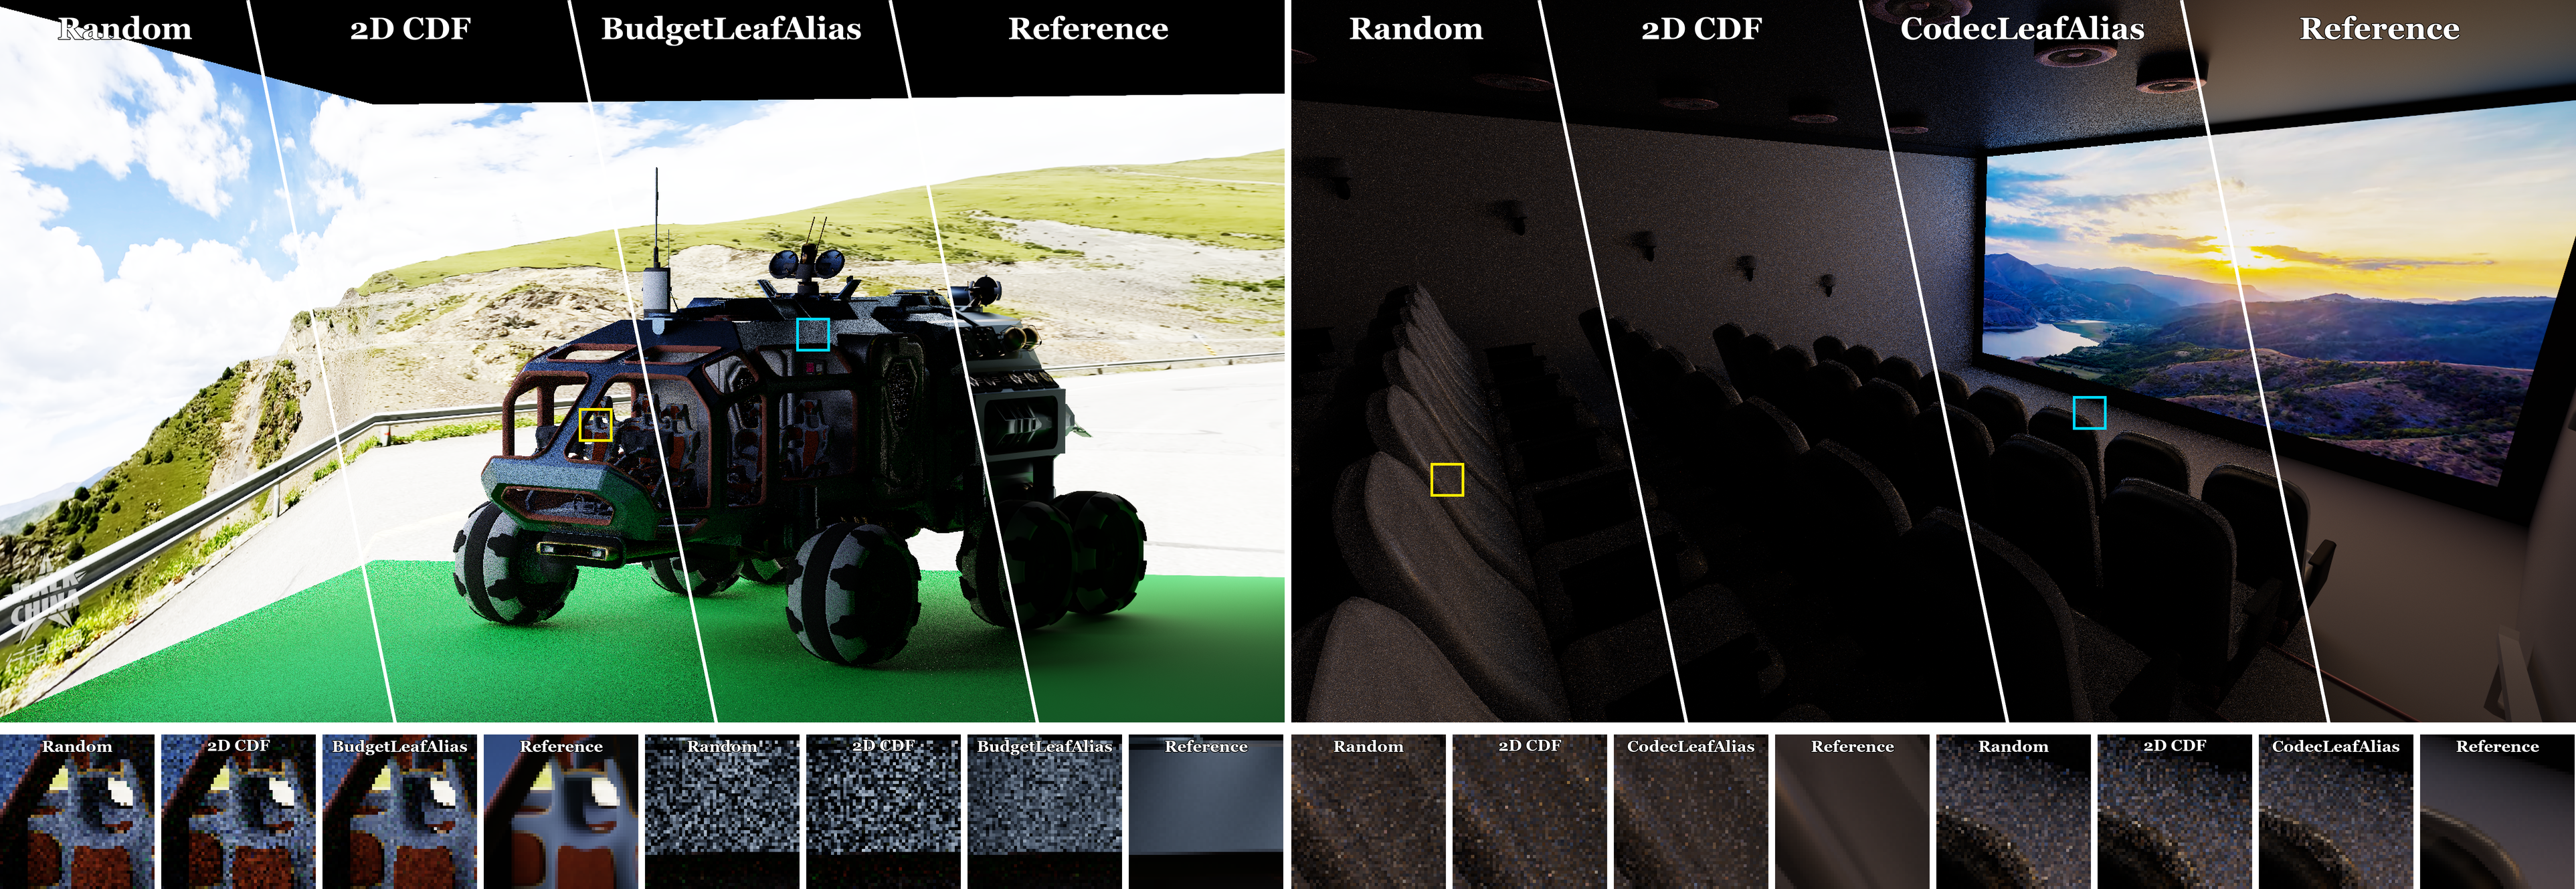
\includegraphics[width=1\textwidth]{teaser.png}
  \caption{Two scenes lit by a single dynamic, video-driven emissive texture, rendered with our LeafAlias importance sampler. (Left) The Rover scene — a virtual-production LED wall displaying a looping road/mountain video panorama that lights the vehicle directly, sampled here with BudgetLeafAlias. (Right) The Cinema scene — a theater lit only by the animated sunset footage playing on its own screen, sampled with CodecLeafAlias. Each panel compares, left to right: Random sampling, 2D CDF inversion, our technique, and a converged reference, all at their calibrated real-time budgets ($\approx$33 ms).}
  \label{fig:teaser}
\end{teaserfigure}

%%
%% This command processes the author and affiliation and title
%% information and builds the first part of the formatted document.
\maketitle

\section{Introduction}

Importance sampling of emissive textures is essential for efficient image-based lighting, and increasingly critical in production and VFX workflows where video is used directly as a dynamic light source. A single emissive texture lets a renderer reproduce the directional detail of a real environment far beyond what analytic lights can approximate. Traditionally, this texture has been static: captured once and reused for an entire sequence. However, there are recent use cases such as LED-wall virtual production, AR/VR object insertion, and video-based environment maps that require illumination that changes every frame.

\rev{The texture light samplers found in current renderers are designed for static images.} They rely on offline construction of large sampling structures that are stored and reused. The most common example of this strategy is how rendering and ray tracing toolboxes deal with HDR environment maps. The standard approach is to build a two-dimensional piecewise-constant distribution from the texture's luminance: a marginal CDF over rows and a per-row conditional CDF. The sampler is then inverted via binary search at sample time, which is expensive and produces incoherent memory access. A more recent and well-adopted approach is to generate a mipmap-style hierarchical importance map \cite{clarberg2005wavelet}. At sample time, a hierarchical descent through a mip pyramid
of the texture is performed, recursively choosing one of four children at each level in proportion to their summed weight. This technique is also expensive and requires several iterations per sample, although it is more GPU-friendly because the number of iterations is always the same for each sample, unlike with the binary search. Moreover, the mipmap can be constructed quickly using the existing dedicated hardware on modern GPUs. Both techniques require at least $O(N)$ memory for the sampler, with $N$ being the number of pixels.

Another less used but known technique for sampling emissive textures is the Alias method \cite{burke2004bidirectional}. This technique draws from an arbitrary discrete distribution in $O(1)$ time after an $O(N)$ one-time build, at the cost of losing the CDF's implicit spatial coherence: two adjacent table buckets can alias to two arbitrary, unrelated locations in the original distribution. This fact is known to disrupt stratification or discrepancy reduction of the input point set. It also requires $O(N)$ memory to store the correlation between every pixel. The process for building the Alias table, despite being $O(N)$, is difficult to optimize for real-time construction \cite{lehmann2021weighted}.

We present a new sampling method that is fast to build, produces a sampler that is tiny, \rev{is $O(1)$ to sample, and does not create the structured sample patterns that the per-pixel Alias method can produce.} The core idea is to reuse the variance-driven image partition that is already present in modern video codecs, which already compute hierarchical spatial partitions that adapt to local signal variance \cite{uhrina2024performance}. These structures implicitly encode the spatial distribution
of luminance and high-frequency content (see Fig. \ref{fig:quadtree}). We also propose a variant that builds the partition tree on a budgeted number of leaves, using a  Greedy/best-first tree-structured resource allocation strategy \cite{MINASNY2007383,Zhou2024}. \rev{Both techniques render video light textures in real time (33 milliseconds per frame) with consistent gains, because each of their samples is cheaper and more of them fit in the frame.}

\newbegin
Our samplers are per frame by design: each frame's structure is built from that frame alone, with no knowledge of past or future frames. Their purpose is not to sample a frame more accurately than an exact per-texel distribution, which is not possible, but to approach its accuracy with a structure that is orders of magnitude smaller and cheaper to build and to sample. Our contributions are:
\begin{itemize}
\item LeafAlias, an alias table over the leaves of a variance-driven partition of the texture, with $O(1)$ sampling and an $O(1)$ density lookup for multiple importance sampling, in a structure of tens of kilobytes.
\item Two sources for the partition: the coding tree of a video codec, with a study of how leaf radiance is obtained from coded data and how quantization, bitrate, codec family and encoder configuration affect it; and a greedy quadtree with a fixed leaf budget.
\item An evaluation that separates the quality of the sampling density (equal samples) from its cost (equal quality), over full videos and against per-texel baselines, together with studies of the leaf budget and its relation to the GPU cache, of static against per-frame partitions, and of temporal stability.
\end{itemize}
\newend

\begin{figure}[htbp!]
  \centering
  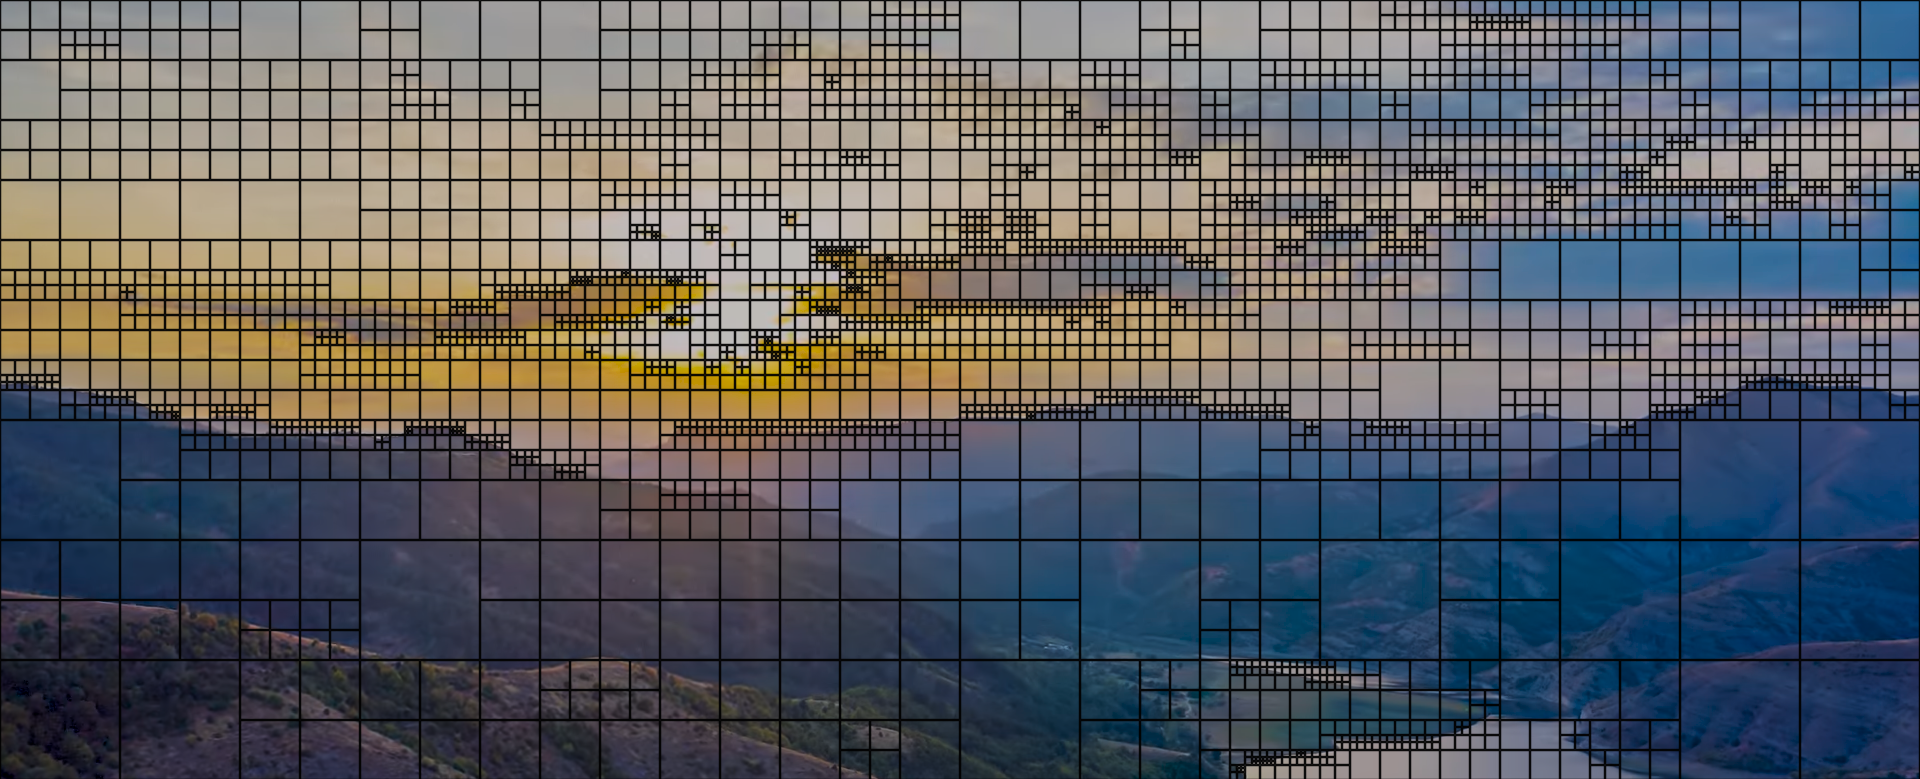
\includegraphics[width=\linewidth]{quadtree.png}
  \caption{An example of a variance-driven quadtree built by the VP9 video codec. High-variance zones are refined into a dense mesh of
  small cells.}
  \label{fig:quadtree}
\end{figure}

\new{
\section{Motivation}

\paragraph{Real-time path tracing in games.}
Light sampling with spatiotemporal resampling draws its initial candidates from
tabulated distributions over emissive geometry and environment maps
\cite{bitterli2020spatiotemporal}, and the cost of rebuilding those tables is a known
obstacle to dynamic content. Wyman and Panteleev~\cite{wyman2021rearchitecting} report the cost of
alias-table builds for large environment maps as one of the main challenges in presampling lights, and instead propose
a GPU-accelerated MIP structure to process textures coming from light probes streamed live from a 360 camera. The quality
of these initial candidates still bounds the result and limits resampling \cite{zeng2025restirpg}, and the integration
of ReSTIR in a shipped path-traced game lists initial candidate sampling quality among
its main sensitivities, with emissive surfaces and the skylight left to BSDF sampling
\cite{kozlowski2023cyberpunk}. Production engines report the same pressure from
content. Lumen lights scenes with emissive surfaces but notes how small
and bright areas cause noise artifacts, and names
explicit sampling of emissive meshes as future work \cite{wright2022lumen}; its
successor for direct lighting observes that artists now use rectangular and textured
lights more frequently \cite{narkowicz2025megalights}. Current guidance for path-traced
games recommends environment maps that are baked every frame so that dynamic skies and
clouds can be importance sampled, and a dedicated sampling structure for signs,
animated effects and procedural emissive materials \cite{nvidia2026ptwhitepaper}.
Recent work still describes the evaluation of many lights per pixel as a major
bottleneck of real-time rendering \cite{chen2026lightopt}.

\paragraph{Virtual production.}
On an LED stage the wall is at once the in-camera background and the light source of
the scene: the stage is driven as an image-based lighting instrument
\cite{debevec2022dilation,legendre2022jointly}, and the video that
drives the wall also drives the lighting fixtures around it \cite{bengtsson2022ibl}.
While the camera rolls, the panels light the real actors physically. The rendering
problem appears whenever the subject under that light is synthetic, and this happens
at three points of a production. Before the shoot, the lighting of a volume is designed
in simulation: productions go through a prelight in the virtual art department, where
the engine reproduces the environment as it will appear on the screens
\cite{kadner2023stages,zwerman2023ves}, techvis rebuilds the on-set hardware as a 3D
scene \cite{failes2024hotd}, and digitized performers are previsualized inside the
virtual stage \cite{nash2025integration}. Such previsualization of panel-generated lighting effects is older than the LED volume \cite{bunish2017rogueone,seymour2013gravity,hamon2014gravity}. During the shoot, when a shot cannot be finished
in camera, the camera frustum is keyed and provisional imagery is composited live
while the rest of the wall keeps lighting the subjects \cite{kadner2021fieldguide}.
After the shoot, the creatures and environments of such shots are added in post
\cite{failes2022hotd} and have to match the lighting that the wall gave the actors.
Research has started to treat the wall accordingly, as a near-field, high-resolution
textured emitter whose image is known at every frame \cite{azzarelli2026relightable},
and to use LED stages to reproduce per-frame HDR environment maps at video rate
\cite{zhang2026pixelcube}. In all of these cases a renderer lights a synthetic subject
with a video, and its sampling structure has to follow that video frame by frame.

\paragraph{Mixed reality and telepresence.}
In augmented and mixed reality the illumination is captured
or estimated while the application runs. HDR environment maps are inferred from the
camera feed at interactive rates on mobile devices
\cite{legendre2019deeplight,somanath2021hdr,zhao2021xihe}, estimated consistently over
video \cite{li2023spatiotemporally,shen2025stglight,bolduc2026limo}, or taken directly
from a live $360^\circ$ stream with changing real-world lights
\cite{rhee2017mr360,rhee2018mr360live,walton2018dynamic}. For such high-frequency
illumination, importance sampling of the environment map is essential for efficient
rendering \cite{kronander2015photorealistic,alhakamy2020realtime}. Systems that do
path trace under a live panorama on a head-mounted display report that the result must
be denoised \cite{cheng2023environment,wu2024panoramic}, and that in a headset Monte
Carlo noise is more than a quality problem, since its temporal flicker aggravates
cybersickness \cite{taibo2024immersive}. Most real-time systems therefore avoid
sampling: they prefilter the map or reduce it to a few dominant lights\cite{saito2024relightable}. A sampling structure that can be rebuilt at
the rate of the display, and that is small enough to keep one per light, is a
precondition for moving these applications from prefiltered shading to path tracing
with correct shadows and interreflections.
}
\section{Previous works}\label{sec:prev}
Importance sampling of emissive textures is a well-studied problem in the graphics literature in the context of image-based lighting. Most of the works focus on preprocessing the images to allow for exact or near-exact sampling without introducing bias \cite{lawrence2005adaptive}. Several methods choose to simplify the textured light into a set of point or area lights ~\cite{agarwal2003structured}, allowing for real-time sampling and faster convergence but at the cost of more error in the solution. \cite{cline2009tabular} compare several tabular inversion methods, noting the computational order of building each sampler structure and sampling each point. They analyze the 2D CDF inversion via binary search and the per-pixel Alias method, where they flag the disruption of the stratification of the input point set. \rev{With a low-discrepancy input, the raster-flattened table of the per-pixel Alias method can produce a measurable periodic banding pattern (Figure~\ref{fig:spectrum}) that becomes clear in the power spectrum of the sample set. Appendix~\ref{app:qmc} analyzes these effects and their consequence in a rendering for our proposed methods and compares it with per-pixel Alais.}

\begin{figure}[htbp!]
  \centering
  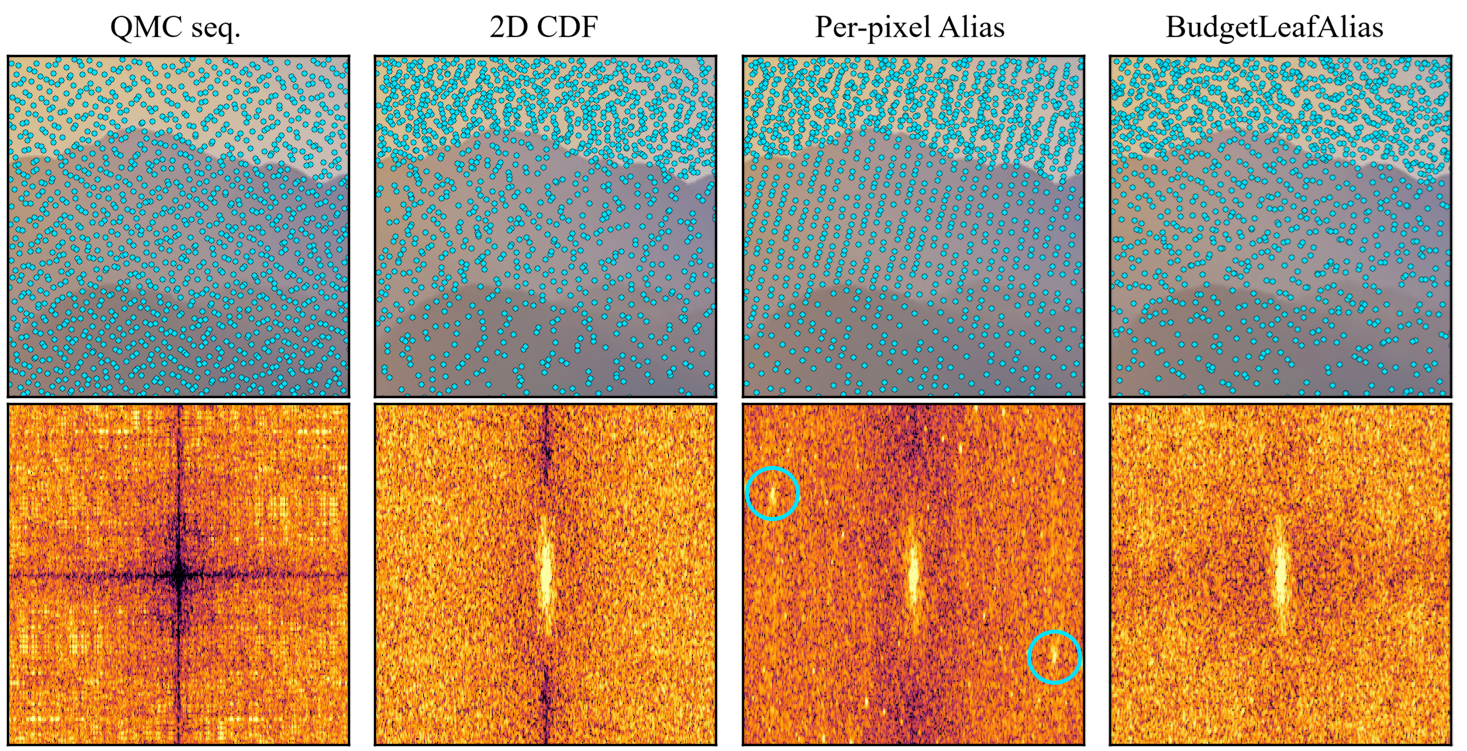
\includegraphics[width=\linewidth]{fig_spectrum_paper_color.png}
  \caption{2D power spectrum of samples from 2D CDF inversion, plain per-pixel alias, and
  our LeafAlias, from the same Halton input. Per-pixel alias shows a sharp,
  isolated off-axis peak (flatness 0.270, peak/median 16{,}113), a periodic banding
  artifact from its flat array index resonating with the input sequence's base-2 digit
  structure.}
  \label{fig:spectrum}
\end{figure}

Despite being $O(1)$ to sample, the Alias method is memory-intensive and expensive to construct via Vose's technique.
Nevertheless, it is widely used in mesh light sampling for geometry with thousands of emissive triangles. \cite{moreau2019dynamic} maintain a light-sampling BVH incrementally across frames for thousands of moving lights.
ReSTIR~\cite{bitterli2020spatiotemporal} resamples across spatial and
temporal neighbors to pick among many dynamic lights at a fraction of the cost of resampling
from scratch. Conty Estevez and Kulla~\cite{contykulla2018adaptive} adaptively split a light
tree per shading point rather than committing to one fixed cut. At that scale of thousands of triangles, a plain alias table over per-triangle flux is common practice
and cheap to rebuild every frame.

Regarding the optimization of the sampling structures,
\cite{ergun2012realtime} split an environment map into a kd-tree via the greedy partition strategy, to a predefined block count, then fit the sorted leaf probabilities with an approximate analytic curve for direct inversion. They report gains in memory compression, higher speed and accuracy than CDF inversion at matched performance for static environment maps. One disadvantage of using kd-trees is that evaluating the pdf of the map direction when sampled from the BRDF in multiple importance sampling (MIS) requires traversing the tree.
 Lambers~\cite{lambers2022parameterization} proposes a fixed-grid sampler and notes that replacing the grid with a variance-driven quadtree might improve their results. \cite{rodriguez2023nenv} train a neural normalizing flow that allows both sampling and evaluating the pdf, showing considerable performance gains at the cost of pre-training the structure for the static map. Wu~\cite{wu2025efficient} also preprocesses the map by dividing the emissive and non-emissive parts into separate structures. \new{Sz\'ecsi et al.~\cite{szecsi2010adaptive} adapt the placement of the samples of an environment map on the GPU, taking the reflectance at the shading point into account as well as the illumination. Sampling densities that depend on the shading point, like \cite{szecsi2010adaptive}, MIS-compensated distributions~\cite{karlik2019mis} or variance-aware guiding~\cite{rath2020variance}, are complementary to our work, which builds a scene-independent density from the texture alone.}

\rev{The previously described techniques focus mainly on preprocessing static images to improve sampling efficiency. Sampling of dynamic environment maps has also been studied.} \new{Wan et al.~\cite{wan2005q2tree} subdivide the sphere into a Q2-tree of quadrilaterals according to illumination importance and generate a temporally coherent set of directional samples for every frame of an environment sequence. Wan et al.~\cite{wan2011spatiotemporal} treat the whole sequence as a spatiotemporal volume and stratify the samples in space and time, and Yang et al.~\cite{yang2014high} extend this line to high-dynamic-range sequences. These methods exploit temporal coherence, and the spatiotemporal ones analyze the sequence as a whole before rendering, which suits recorded content. Our method works on the current frame only, so it applies to live video, and it produces a density that can be sampled and evaluated for MIS inside a path tracer, rather than a fixed set of light directions.} \rev{Other works address video-driven lighting:} \cite{havran2005interactive} and Iorns and Rhee~\cite{iorns2015realtime} both light scenes from captured video environment maps, but neither targets real-time per-frame
resampling of the video itself as the importance distribution. \cite{lu2013realtime} rebuild a tabulated per-cube-face CDF in real-time, noting it as an expensive part of the process. \cite{kronander2014real} rely on temporal sample reuse to improve convergence of video-based lighting.

Attempts to make the per-frame rebuild itself cheaper on a GPU point in the same direction: Morrical and Zellmann~\cite{morrical2021inverse} accelerate 2D CDF
inversion with ray tracing hardware at a high construction cost and non-trivial implementation
complexity. \cite{lehmann2021weighted} study GPU-specific weighted sampling and alias-table construction directly. \new{Binder and Keller~\cite{binder2019radix} build radix tree forests in parallel on the GPU to sample discrete distributions with a monotone mapping. These approaches make a per-texel structure faster to build; ours reduces the size of the structure instead, which lowers the cost of building it, storing it and sampling it at once.}

Modern production renderers mostly rely on dense CDF or mipmapped samplers. {Falcor}~\cite{falcorsoftware} uses a hierarchical mip-pyramid importance map over the environment texture's luminance and, separately,
the triangle-scale alias table for mesh lights. {Mitsuba 3}~\cite{nimierdavid2019mitsuba2} builds a {Hierarchical2D} warp over
the environment map, which is the same mip-pyramid family as Falcor's. {pbrt-v4}~\cite{pharr2023pbrt}
uses a dense CDF distribution, inverted via binary search. {Blender Cycles}~\cite{cyclessoftware} builds the same
kind of dense marginal/conditional CDF over a downsampled background map.

\section{Method}\label{sec:method}

The LeafAlias technique applies to any light source described by a 2D radiance texture $L(u,v)$ over
a parameter domain $(u,v)\in[0,1)^2$, e.g. an environment map, or the emission texture of an
area light. As with any textured light, variance is minimized when the sampling density
matches radiance, $p(u,v)\propto L(u,v)$. We approximate this with a piecewise-constant density
over a partition of the domain into disjoint leaf rectangles $\{R_i\}_{i=1}^N$, for now
assumed given; Sections \ref{sec:codec} and \ref{sec:budget} describe the two ways we
actually construct it. Each leaf carries a single weight proportional to its flux: its area in the parameter domain
times its average radiance:
\begin{equation}
w_i = A_i \bar{L}_i, \qquad \bar{L}_i = \frac{1}{A_i}\int_{R_i} L(u,v)\,dA. \label{eq:weight}
\end{equation}
Normalizing over all leaves gives a piecewise-constant density over the parameter domain
and a per-leaf selection probability:
\begin{equation}
p(u,v) = \frac{\bar{L}_i}{W} \ \text{for } (u,v) \in R_i, \qquad
p_i = \frac{w_i}{W}, \qquad W = \sum_{j=1}^N w_j. \label{eq:pdf}
\end{equation}
Converting $p(u,v)$ to whatever measure a particular light type actually samples with
respect to (solid angle for a distant environment map or projected solid angle for a local
area light) is a standard change-of-variables applied at evaluation time, and is
independent of the sampling structure described below.

Given the partition, we flatten it into an array of $N$ leaves, each storing its rectangle
and weight $w_i$ from Equation~\ref{eq:weight}. We build a Walker/Vose alias
table~\cite{vose1991linear} over this array once, in $O(N)$: leaves below the mean weight
are paired with leaves above it, the excess of the latter absorbs the deficit of the
former, and the process repeats until every leaf holds a threshold and, where needed, the
index of the leaf it aliases to (Algorithm~\ref{alg:build}). Unlike a dense CDF, the
resulting table needs no search at sample time since selecting a leaf is an $O(1)$ array
lookup.

\begin{algorithm}[h]
\caption{Build the alias table over $N$ leaves}
\label{alg:build}
\begin{algorithmic}[1]
\STATE $W \leftarrow \text{mean}(w_1,\dots,w_N)$
\STATE partition leaf indices into \textit{small} ($w_i < W$) and \textit{large} ($w_i \geq W$)
\WHILE{\textit{small} and \textit{large} both non-empty}
  \STATE $s \leftarrow$ pop(\textit{small}); \quad $l \leftarrow$ pop(\textit{large})
  \STATE $\mathit{threshold}[s] \leftarrow w_s / W$; \quad $\mathit{alias}[s] \leftarrow l$
  \STATE $w_l \leftarrow w_l - (W - w_s)$ \COMMENT{transfer $l$'s excess weight to $s$}
  \STATE push $l$ back onto \textit{small} or \textit{large} by its updated $w_l$
\ENDWHILE
\FOR{remaining $i$ in \textit{small} $\cup$ \textit{large}}
  \STATE $\mathit{threshold}[i] \leftarrow 1$
\ENDFOR
\end{algorithmic}
\end{algorithm}

\subsection{Sampling}
\label{sec:sampling}
To draw a light sample, we use three uniform numbers $\xi_1,\xi_2,\xi_3$
(Algorithm~\ref{alg:sample}). $\xi_1$ selects a bucket in $O(1)$;
$\xi_2$ decides whether we keep that leaf or its
alias partner.
$\xi_3$ and $f$ place the sample uniformly
inside the chosen leaf's rectangle. The sample's pdf is read directly from its
leaf's stored average luminance via Equation~\ref{eq:pdf}. Radiance is read from the texture at the sampled $(u,v)$.

\begin{algorithm}[h]
\caption{Draw one light sample}
\label{alg:sample}
\begin{algorithmic}[1]
\STATE $i \leftarrow \lfloor \xi_1 N \rfloor$; \quad $f \leftarrow \xi_1 N - i$
\IF{$\xi_2 < \mathit{threshold}[i]$}
  \STATE $\mathit{leaf} \leftarrow i$
\ELSE
  \STATE $\mathit{leaf} \leftarrow \mathit{alias}[i]$
\ENDIF
\STATE $(u,v) \leftarrow \text{lerp}(R_{\mathit{leaf}}.\mathit{min}, R_{\mathit{leaf}}.\mathit{max},\, (f,\xi_3))$
\STATE \textbf{return} $(u,v)$, $\;p(y){=}\bar{L}_{\mathit{leaf}}/W$ (Eq.~\ref{eq:pdf}), $\;L(u,v)$
\end{algorithmic}
\end{algorithm}

Combining light sampling with BRDF sampling via MIS requires the
reverse query: given a direction chosen by BRDF sampling that happens to hit the light at
some $(u,v)$, the probability $p(y)$ is needed. Rather than searching the partition, we
maintain a small auxiliary lookup matrix that maps a coarsened $(u,v)$ coordinate directly to
its leaf index, at a fixed fraction of the texture's resolution matching the partition's
smallest possible leaf (e.g.\ one entry per $8{\times}8$ block).
Every coordinate covered by a given leaf is written to the same entry at
construction time, so the lookup is an $O(1)$ array read that reproduces the exact same
$\bar{L}_i/W$ used at sampling time regardless of that leaf's actual size, keeping the
resulting MIS weight unbiased. We also tried replacing this exact lookup with a single
scene-wide average density: across our test scenes this produced no perceptible difference
in the rendered images, but it does introduce bias, since the substituted value no longer
matches the technique's actual density at that point.

\subsection{CodecLeafAlias}
\label{sec:codec}
Building the partition can be costly, especially for dynamic content that changes every few milliseconds.
CodecLeafAlias avoids it entirely when the texture
arrives as a compressed video frame. Modern codecs (HEVC, AV1, VP9) already split each frame
into a coding-tree hierarchy driven by local signal variance, which is structurally the same
partition our method needs.
We take each coding-tree leaf's block directly as one of our leaf rectangles $R_i$, and
estimate $\bar{L}_i$ from the block's own zero-frequency (DC) transform coefficient rather
than summing pixels: the DCT/DST's DC term is, up to a fixed normalization constant, exactly
the block's mean sample value, and is already computed and present in decoder metadata.
\newbegin
The DC coefficient gives the mean of a block of the \emph{coded} signal, which for HDR video is a nonlinear, quantized $Y'C_bC_r$ signal (10-bit PQ, BT.2100, in our experiments), so three steps separate it from $\bar{L}_i$. (1)~The reconstructed block mean of each plane is its dequantized DC divided by the transform gain. For a block coded with prediction, the DC belongs to the residual, and the mean of the prediction (extracted from the decoding process) must be added. (2)~The three means are converted to $R'G'B'$ with the BT.2020 matrix, linearized with the PQ transfer function, and transformed to luminance with the BT.2020 weights. (3)~The result is multiplied by the leaf area to give $w_i$ (Eq.~\ref{eq:weight}). This process and quantization perturb the DC, and therefore the density of Eq.~\ref{eq:pdf}, but not the expected value of the estimator: every sample is divided by the density actually used, so the estimate stays unbiased for any density that is positive wherever the emitter is. We keep a small density floor ($10^{-4}$ of the mean weight) so that no lit leaf is quantized to zero. A wrong weight can therefore only add variance; Section~\ref{sec:codecstudy} measures the effect of quantization in the results.
\newend

In our experiments, we encode the dynamic emissive textures as HDR video using libvpx's VP9 Profile 2 and extract the superblocks for each frame via decoder statistics. We configure the encoder to always use variance-based superblock partitioning. Encoder settings that instead search or reuse partitions (full rate-distortion search, predicted neural partitions, etc.) \new{can} still supply a usable partition by combining each block's motion vector with its keyframe's already-computed superblocks. \new{Section~\ref{sec:codecstudy} evaluates this strategy, other codec families and the effect of bitrate.} 

Using codec partitions results in varying number of leaves, ranging from 4000 to 20000 depending on the content. We call this method CodecLeafAlias. Since the sampling algorithms are memory-bound operations, we go further by defining a new partition mechanism that allows us to choose a budgeted number of leaves to reduce memory needs and improve coherence. We call this other method BudgetLeafAlias.

\subsection{BudgetLeafAlias}
\label{sec:budget}
BudgetLeafAlias constructs the quadtree directly from the texture under a hard
leaf-count budget $B$ (in our implementation, matched to what fits alongside the alias
table in a modern GPU's L1 data cache; Section~\ref{sec:impl}). Rather than recursing to a
fixed depth or a fixed per-node threshold, we spend the budget greedily
(Algorithm~\ref{alg:budget}): a priority queue always refines whichever pending block
currently contributes the most summed-squared error to the piecewise-constant
approximation, $\mathrm{Var}(R)\cdot A(R)$, until the budget is exhausted or no block has
positive variance left to resolve. This is the standard greedy construction for a
budget-constrained piecewise-constant approximation: unlike a fixed-depth or
fixed-threshold rule, it spends every one of its $B$ leaves wherever the source image
actually has the most error left to remove.

\begin{algorithm}[h]
\caption{Build a budgeted quadtree of $\leq B$ leaves}
\label{alg:budget}
\begin{algorithmic}[1]
\STATE $\mathit{queue} \leftarrow \{\mathit{root}\}$; \quad $\mathit{leaves} \leftarrow \emptyset$
\WHILE{$\mathit{queue} \neq \emptyset$ and $|\mathit{leaves}| + |\mathit{queue}| + 3 \leq B$}
  \STATE $R \leftarrow$ pop block with max $\mathrm{Var}(R)\cdot A(R)$ from $\mathit{queue}$
  \FOR{each of the 4 children $C$ of $R$}
    \IF{$C$ is $8{\times}8$ texels or smaller, or $\mathrm{Var}(C) = 0$}
      \STATE $\mathit{leaves} \leftarrow \mathit{leaves} \cup \{C\}$
    \ELSE
      \STATE $\mathit{queue} \leftarrow \mathit{queue} \cup \{C\}$
    \ENDIF
  \ENDFOR
\ENDWHILE
\STATE $\mathit{leaves} \leftarrow \mathit{leaves} \cup \mathit{queue}$
\end{algorithmic}
\end{algorithm}

\subsection{Implementation}
\label{sec:impl}
\rev{We implement both variants in NVIDIA's Falcor rendering engine and test using a full path tracer with MIS: one BSDF sample per bounce, and a configurable number of light samples per shading point, each weighted against BSDF sampling.}
We construct the LeafAlias tables and partitions in the CPU, and pass the results to the GPU in each frame.
All the precomputation is done in under 1 millisecond per frame. We implement the sampling method in the Slang Shading Language.
In order to reduce GPU memory usage and improve coherency, we spent some effort in making the sampling structures as small as possible.
Each leaf is packed into a 16-byte record, its rectangle as two packed 16-bit corner coordinates, the alias threshold and redirect index
as a half-float and a 16-bit index, and $\bar{L}_i$ as a half-float. For BudgetLeafAlias, we size $B$ so the combined leaf and node buffers fit within roughly half of the GPU's per-core L1 cache, keeping the whole sampling structure resident there during
traversal instead of round-tripping to global memory on every sample. \rev{With $B=4000$ the structure takes 75\,KB. This compactness helps improve performance when compared to other memory-bound samplers like dense CDF or per-pixel Alias table; Section~\ref{sec:leafbudget} measures the effect of $B$ on quality and on cost.}

\section{Results} \label{sec:results}

All experiments run on an Intel Core i7-14700F CPU and an NVIDIA GeForce RTX 4080 SUPER GPU (128\,kB of L1 cache/shared memory per streaming
multiprocessor). We evaluate seven real-time techniques across our five scenes
(LED-wall Rover, projector-lit Cinema, Fireplace Room, Phone, and the multi-material
Convergence scene): uniform random sampling; dense 2D CDF inversion; the same CDF built at $1/8$ resolution; a hierarchical
mipmap-warp sampler; a per-pixel Alias table; and our
own {BudgetLeafAlias} and {CodecLeafAlias}. We added 2D CDF/8 to analyze the quality and performance
tradeoffs of a coarser resolution; we also tested several further resolution-trimming factors beyond $1/8$ (down to $1/16$ and $1/32$)
and observed the same trend: smaller resolutions are cheaper to sample but significant error is introduced. We report only the $1/8$ variant in what follows, as the representative trimmed-resolution case.

All techniques are implemented in Falcor, with particular
attention paid to making the GPU-side sampling code efficient for each technique. The CPU-side cost
of building each sampling structure for every frame varies considerably: 2D CDF's
dense per-pixel CDF costs approximately $10$\,ms per Full HD frame, while per-pixel Alias table costs approximately $30$\,ms; our own technique's
leaf-budgeted construction is consistently under $1$\,ms per frame across every scene tested. The sampling parameters for each technique (samples per pixel and light samples per vertex) are tuned per scene to a real-time budget of $33$\,ms (30\,fps) using the same calibration procedure. 
 \new{Since we are interested in analyzing the sampler efficiency, not the structures build time, we leave the build time out of the calibration, so the presented real-time results only consider sampling performance. }
2D CDF and mipmapped methods allow approximately a third of the samples obtained with the random approach. BudgetLeafAlias allows the same number of samples as random, while CodecLeafAlias and per-pixel alias allow approximately 25\% fewer. \new{Table~\ref{tab:configs} lists the configurations. BudgetLeafAlias uses $B=4000$ leaves unless stated otherwise.}

\begin{table}[htbp!]
\centering\small\newmat
\setlength{\tabcolsep}{3pt}
\caption{\newmat Calibrated real-time configuration of each technique per scene: samples per pixel $\times$ light samples per shading point, each within the 33\,ms frame. }
\label{tab:configs}
\resizebox{\columnwidth}{!}{%
\begin{tabular}{l ccccccc}
\toprule
Scene & \shortstack{Random} & \shortstack{2D CDF} & \shortstack{2D CDF/8} & \shortstack{Mipmap} & \shortstack{Per-pixel\\Alias} & \shortstack{Budget\\LeafAlias} & \shortstack{Codec\\LeafAlias} \\
\midrule
Rover & 4$\times$19 & 4$\times$5 & 4$\times$12 & 4$\times$9 & 4$\times$13 & {4$\times$19} & 4$\times$15 \\
Cinema & 4$\times$8 & 4$\times$2 & 4$\times$4 & 4$\times$3 & 4$\times$5 & {4$\times$8} & {4$\times$8} \\
Fireplace Room & 4$\times$5 & 4$\times$2 & 4$\times$2 & 4$\times$2 & 4$\times$3 & {4$\times$5} & {4$\times$4} \\
Phone & 16$\times$10 & 16$\times$3 & 16$\times$5 & 16$\times$3 & 16$\times$7 & {16$\times$10} & {16$\times$8} \\
Convergence & 4$\times$3 & 4$\times$1 & 4$\times$2 & 4$\times$1 & 4$\times$2 & {4$\times$3} & {4$\times$3} \\
\bottomrule
\end{tabular}}
\end{table}

Each scene is lit by a different HDR video played back as the
scene's only light source: Rover uses a Full HD road/mountain driving sequence
(600 frames) displayed on a virtual-production LED wall; Cinema uses a Full HD
sunset-landscape sequence (250 frames) with a small, very bright sun; Fireplace Room uses a 4K real fire video (800 frames); Phone uses
a Full HD abstract color sequence (1200 frames); and
Convergence uses a 4K dark cave with multiple bright lights video (800 frames) as a single environment map. Altogether, across these five sequences, our techniques are evaluated against thousands of distinct HDR emissive
textures, not just the one representative frame shown in each figure. The resulting videos are found in the supplementary material.

\new{The evaluation is organized around three questions. Section~\ref{sec:video} reports the quality of every technique over the full videos at its real-time configuration. Section~\ref{sec:equalsamples} removes the cost of sampling from the comparison (equal samples), to measure what the leaf approximation loses. Section~\ref{sec:equalquality} measures what its lower cost gains (time to equal quality). The remaining sections analyze the cost itself, the leaf budget, the need for a per-frame partition, and the codec variant.}

\subsection{\texorpdfstring{\revt{Full-video quality}}{Full-video quality}}
\label{sec:video}

\newbegin
For each scene we render regularly spaced frames spanning the whole video. Each frame is compared with a converged reference of the same frame, without denoising. RMSE is computed per frame on the tone-mapped output and averaged over frames, as well as PSNR; VMAF is computed on the frame sequence of each technique against the reference sequence. We report each mean with its 95\% confidence interval over frames.

Table~\ref{tab:main} reports RMSE, PSNR and VMAF for all seven techniques on all five scenes. On every scene, one of our two techniques has the best mean on all three metrics: BudgetLeafAlias on Rover, Cinema and Phone, CodecLeafAlias on Fireplace Room and Convergence. Relative to the 2D CDF, the best of our two techniques lowers the video RMSE by up to 23\%. The gains hold over the whole video and appear in the perceptual metric as well: on Convergence, VMAF rises from 54.5 with the 2D CDF to 61.5 with CodecLeafAlias.

\input{table_video_all.tex}

\newend

In order to analyze the real-time performance of each technique, Figure~\ref{fig:realtime} plots the fitted curves of quality as a function of frame processing time. BudgetLeafAlias's curve stays below both structured baselines, 2D CDF and Mipmap for every scene. Its
curve is also consistently the steepest of the three, so the advantage widens as more time
becomes available.

\begin{figure*}[htbp!]
  \centering
  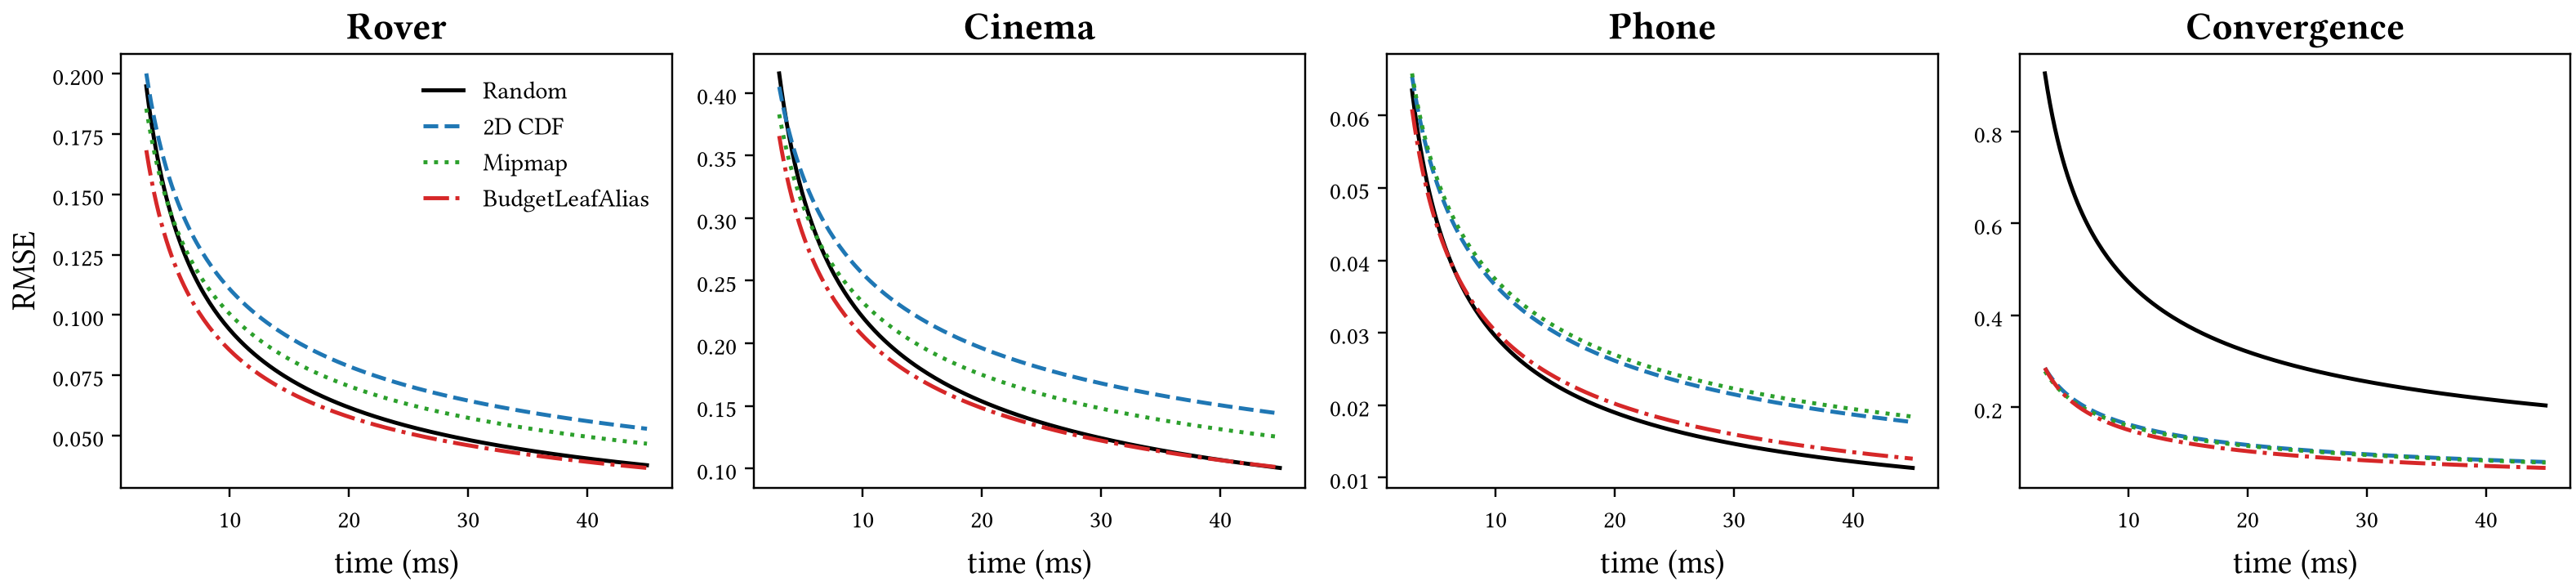
\includegraphics[width=\textwidth]{realtime_curves.png}
  \caption{Fitted RMSE-vs-time curves for Rover, Cinema, Phone, and Convergence, and all four
  techniques. BudgetLeafAlias (red) stays below both 2D CDF
  (blue) and Mipmap (green) across the entire measured range on every scene. }
  \label{fig:realtime}
\end{figure*}

\subsection{\texorpdfstring{\newt{Comparison at equal samples}}{Equal samples}}
\label{sec:equalsamples}

\newbegin
This experiment compares the techniques at the same number of samples for each scene: 4 spp and 2 light samples per vertex. We aim at measuring the variance introduced by using the LeafAlias technique. All techniques render the representative frame of each scene, 24 times with independent random numbers, and the results are compared against a converged reference (Figure~\ref{fig:equalsamples}). The three techniques that importance sample the emitter at full texel resolution (the 2D CDF, the mipmap warp and the per-pixel Alias table) reach the same error within 1\% on every scene. They sample the same distribution and differ only in how they invert it, so at equal samples, and with the independent random numbers of our renderer, they are expected to coincide. Random sampling is clearly worse: its RMSE is 1.12 and 1.21 times that of the 2D CDF on Rover and Cinema, and 1.55, 2.23 and 2.37 times on Phone, Fireplace Room and Convergence. The 2D CDF at $1/8$ resolution is up to 2.6\% behind the full-resolution techniques.

\begin{figure}[htbp!]
  \centering
  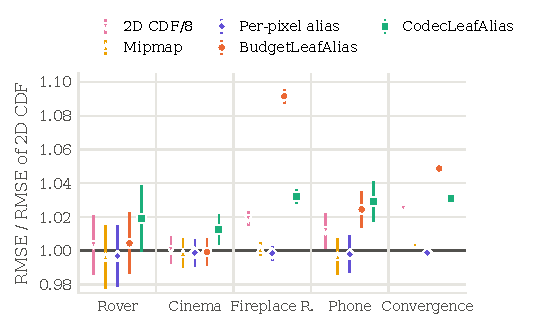
\includegraphics[width=\columnwidth]{fig_equal_samples.pdf}
  \caption{\newmat RMSE of each technique relative to the 2D CDF, with every technique using the same samples per pixel and light samples per shading point (mean of 24 renders, 95\% intervals). Random sampling, at 1.12 to 2.37, is outside the plotted range. }
  \label{fig:equalsamples}
\end{figure}

Our two techniques are slightly behind the full-resolution techniques. Relative to the 2D CDF, the RMSE of BudgetLeafAlias is $+0.4\%$ on Rover, $-0.2\%$ on Cinema, $+2.5\%$ on Phone, $+4.9\%$ on Convergence and $+9.2\%$ on Fireplace Room; that of CodecLeafAlias is $+1.2$ to $+3.3\%$ on all five scenes. The cause is the resolution of the density: both techniques choose a leaf in proportion to its mean luminance and then a point uniformly within the leaf, so the variation of luminance inside a leaf is not importance sampled. CodecLeafAlias has more and smaller leaves on such detailed content and loses less there, but its partition follows image detail rather than light, so it also spends leaves where they do not help. Figure \ref{fig:closeupsequalsamples} shows some rendering closeups for different techniques under the same number of samples.

\begin{figure}[htbp!]
  \centering
  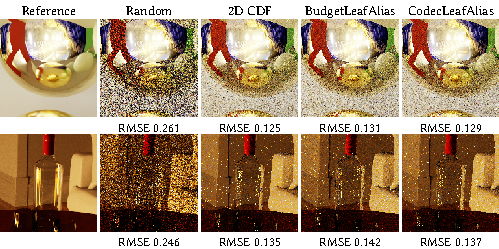
\includegraphics[width=\columnwidth]{closeup_examples.pdf}
  \caption{\newmat Examples of rendering closeups under different techniques with the same number of samples on the Convergence and Fireplace Room scenes.   }
  \label{fig:closeupsequalsamples}
\end{figure}

At equal samples, therefore, our techniques do not sample better than a texel-resolution distribution, and are not meant to: they trade a small loss of sampling quality for a much lower cost per sample and per frame.
\newend

\subsection{\texorpdfstring{\newt{Comparison at equal quality}}{Equal quality}}
\label{sec:equalquality}

\newbegin
In this experiment, we measure how long does each technique need to reach the quality that the 2D CDF delivers in real-time. 
For each scene we render the videos only with direct illumination, where the light sampler controls most of the noise. The 2D CDF uses the number of light samples that fits a 33.3\,ms frame. Every other technique is rendered with several numbers of light samples, and we find the frame time at which its video RMSE equals that of the 2D CDF. The speed-up is the frame time of the 2D CDF divided by that time.

Our two techniques reach the quality of the 2D CDF faster on all five scenes (Table~\ref{tab:equalquality}). These figures use the median frame time of each technique over several timing passes. The other techniques are not consistent: the mipmap warp is slower than the 2D CDF on Rover and does not reach its quality on Phone at the measured sample counts, and the per-pixel Alias table, which is fast on Full HD emitters, is slower than the 2D CDF on the two scenes with 4K emitters, where its memory consumption grows considerably. The time saved can be returned to the frame rate, to more bounces, or to a denoiser.

\begin{table}[htbp!]
\centering\small\newmat
\setlength{\tabcolsep}{3pt}
\caption{\newmat Speed-up of the different techniques over 2D CDF to reach the same average RMSE in the full video.}
\label{tab:equalquality}
\resizebox{\columnwidth}{!}{%
\begin{tabular}{l c c c c c}
\toprule
Technique & Rover & Cinema & Fireplace R. & Phone & Convergence \\
\midrule
2D CDF/8 & 1.17 & 1.89 & 1.29 & 1.17 & 1.17 \\
Mipmap & 0.85 & 1.45 & 1.10 & -- & 1.06 \\
Per-pixel Alias & 1.17 & 1.91 & 0.91 & 1.26 & 0.93 \\
BudgetLeafAlias & 1.31 & 2.23 & 1.19 & \textbf{1.47} & 1.27 \\
CodecLeafAlias & \textbf{1.38} & \textbf{2.31} & \textbf{1.54} & 1.23 & \textbf{1.37} \\
\bottomrule
\end{tabular}}
\end{table}

\paragraph{Emitter resolution}
The last observation suggests that the resolution of the emitter influences the advantage of our techniques. To isolate it, we render using the same emissive texture at three resolutions on the LED wall of the Rover scene: 1820$\times$1024, 3640$\times$2048 and 7280$\times$4096, obtained by area averaging from a real 8K HDR panorama of a road under broad daylight. We render frames with direct illumination, measuring time and RMSE at varying samples per pixel, and smooth the RMSE curve of each technique with a quadratic fit (Figure~\ref{fig:wall}).

\begin{figure}[htbp!]
  \centering
  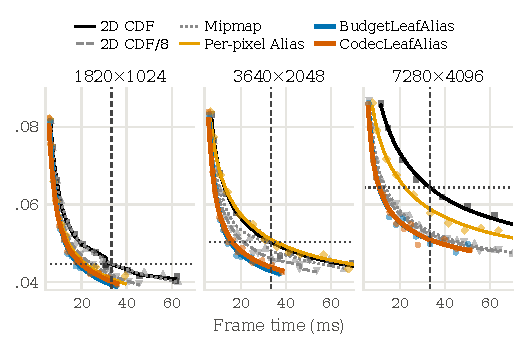
\includegraphics[width=\columnwidth]{fig_wall.pdf}
  \caption{\newmat The same image on the LED wall of the Rover scene at three resolutions: RMSE against frame time (markers: measurements; curves: fits). The vertical line is the 33.3\,ms budget and the horizontal line the RMSE of the 2D CDF at that budget. As the image grows, the curve of the 2D CDF moves to the right and ours stay almost in place.}
  \label{fig:wall}
\end{figure}

The cost of a light sample grows with resolution for the 2D CDF, and much less for our techniques. Each additional light sample per shading point adds 0.95, 1.17 and 2.93\,ms to the frame of the 2D CDF at the three resolutions, and 0.47, 0.50 and 0.73\,ms to that of BudgetLeafAlias. The 2D CDF searches a table as large as the image, with one dependent memory read per search step, and at 8K that table is sixteen times larger than at Full HD; ours read a table of about 75\,KB at any resolution, and the image only once the texel has been chosen. In a 33.3\,ms frame the 2D CDF therefore fits 34, 25 and 10 light samples, while BudgetLeafAlias fits 60, 58 and 40.

As a result, the speed-up at equal quality grows at 8K: both techniques reach the quality of the 2D CDF up to 3$\times$ faster. Read at equal time, the RMSE of BudgetLeafAlias is 12\%, 15\% and 21\% lower than the 2D CDF's. The per-pixel Alias table follows the 2D CDF, since its table also grows with the image and its memory access patterns are more incoherent. The two baselines that keep small or hierarchical structures, the 2D CDF at one eighth of the resolution and the mipmap warp, scale better and reach 2.67 and 2.44 times at 8K; they remain behind our techniques at every resolution. 
\newend

\subsection{\texorpdfstring{\newt{Sampling cost on the GPU}}{Sampling cost on the GPU}}
\label{sec:cost}

\newbegin
We relate the cost of drawing a light sample to the cache levels of the GPU with two benchmarks (Figure~\ref{fig:cache}). In the left figure, a pointer chase reads memory in a chain of dependent random accesses as the working set grows from 4\,KB to 512\,MB. It shows a sharp limit: dependent reads cost about 3\,ps (in aggregate over the whole GPU) while the data fits in the first-level cache, but three times as much once the working set exceeds 128--192\,KB, and tens of times more beyond the second-level cache (64\,MB on our GPU). 

\begin{figure}[htbp!]
  \centering
  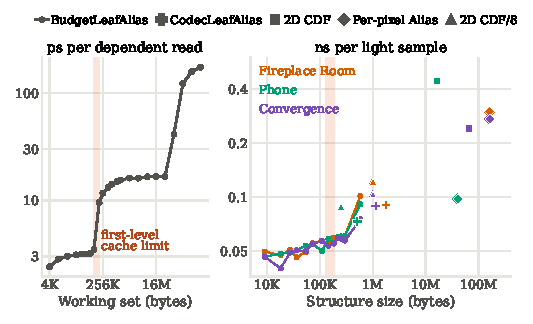
\includegraphics[width=\columnwidth]{fig_gpu_cost2.pdf}
  \caption{\newmat Left: latency of dependent random reads against the size of the data being read, on the GPU (pointer chase, aggregate over the whole GPU). Right: measured cost of one light sample against the size of the sampling structure: BudgetLeafAlias from 64 to 32000 leaves (lines), CodecLeafAlias, and the 2D CDF, per-pixel Alias and 2D CDF/8 (markers), in three scenes. }
  \label{fig:cache}
\end{figure}

In the second figure, we measure the time it takes to draw a sample and read the emissive texture, with varying $B$ values and the other techniques.
The emissive texture read is generally fast because most of the samples point to the same bright sections of the image, hence hitting cache more frequently. These results show the same behavior as the left figure. A sample of the 2D CDF costs between 0.23\,ns and 0.46\,ns, as throughput of the whole GPU, and we give the cost of the other techniques relative to it. BudgetLeafAlias at $B=4000$ is 4 to 8 times cheaper, and its cost hardly changes with the scene; CodecLeafAlias, whose table is larger, costs 1.3 to 1.6 times as much as BudgetLeafAlias. 

The per-pixel Alias table costs a quarter of the 2D CDF on the Full HD emitter of Phone, but 1.2 times as much on the 4K emitter of Convergence. This is explained by the fact that its structure, despite being $O(1)$ to sample, performs two dependent reads per sample at addresses spread uniformly over the whole structure, so almost every read misses the first-level cache; at 4K the structure exceeds the second-level cache as well, and the cost per sample more than doubles.  The 2D CDF performs 24 dependent reads per sample in the worse case, but most of them are cache hits: the marginal CDF is a few kilobytes, and the conditional searches concentrate on the few bright rows.
\newend

\subsection{\texorpdfstring{\newt{Leaf budget}}{Leaf budget}}
\label{sec:leafbudget}

\newbegin
In the next experiment, we sweep the leaf budget $B$ of BudgetLeafAlias from 16 to 16000 leaves in the five scenes at varying number of light samples per pixel. Figure~\ref{fig:leafbudget} shows the error of each budget relative to $B=4000$ at equal samples, so that only the quality of the leaf density is compared.

\begin{figure*}[htbp!]
  \centering
  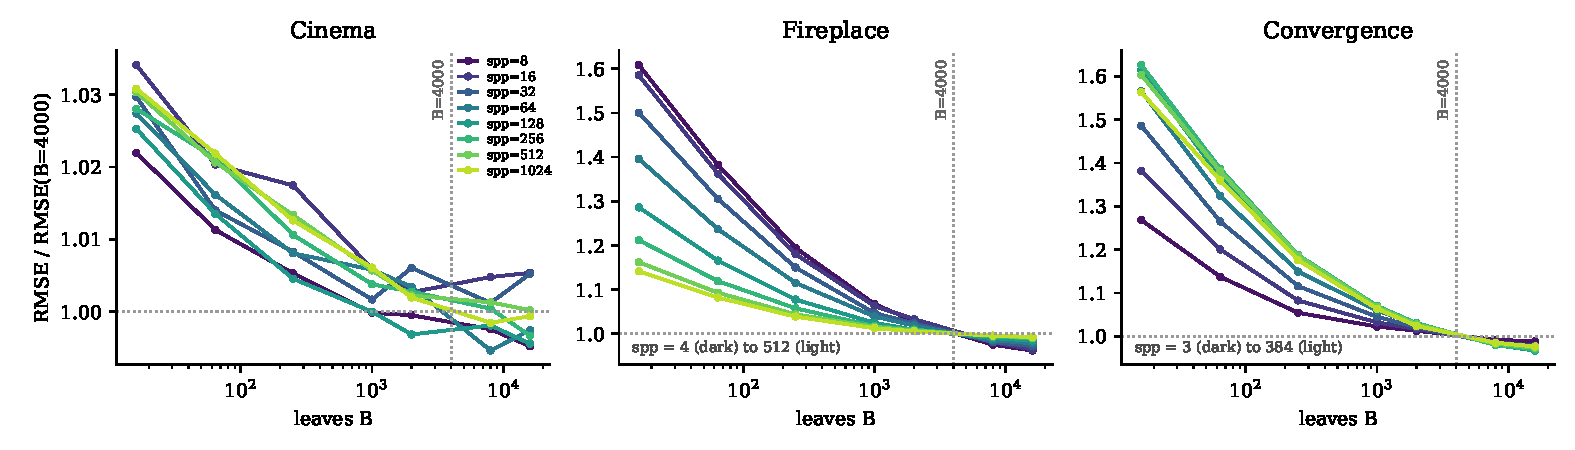
\includegraphics[width=0.92\textwidth]{fig_leaf_budget.pdf}
  \caption{\newmat RMSE against the converged reference, divided by the RMSE of $B=4000$ at the same number of light samples per pixel (spp), as a function of the leaf budget $B$. Values above 1 mean more error than $B=4000$.}
  \label{fig:leafbudget}
\end{figure*}

Two behaviors appear, depending on how the light is distributed over the emitter. In Cinema, light is spread over most of the screen, and a coarse partition already results in one figure error percentages. Rover and Phone behave in a similar way (not shown). In Fireplace Room and Convergence, most of the energy sits in small regions that the partition must resolve, and the error falls steeply with $B$ before levelling off. In Convergence, 250 leaves give up to 1.20 times the error of $B=4000$,  and 1000 leaves up to 1.07 times, while doubling or quadrupling the budget beyond 4000 improves the error by only 1--3\% at every sample count. 

On the cost side, as we saw in the previous section, the structure grows linearly with $B$, and the performance penalty is minimized as long as the sampler resides in L1 cache. $B=4000$ therefore sits at the knee of both curves: it captures nearly all the quality available from the partition, and at 75\,KB it uses most of the cache without exceeding it. $B$ acts as a memory and quality knob, and devices with smaller caches or less memory can use a smaller budget at the quality cost shown in Figure~\ref{fig:leafbudget}. All these measurements are on one GPU; the \supp{ablation\_leaf\_number} contains the complete tables and the  \supp{GPU\_tests} contain results for a mobile GPU device, showing similar patterns when using less cores and memory.
\newend



\subsection{\texorpdfstring{\newt{Frequency of frame partitions}}{Frequency of frame partitions}}
\label{sec:static}

\newbegin
As an alternative to rebuilding the partition every frame, we analyze the error generated by building the tree and leaf weights with less frequency. We compare under equal number of samples: (i)~one tree and one set of weights computed from the average of all frames, with 5\% of the probability spread uniformly to keep the estimator unbiased; (ii)~the same average tree with the weight of each leaf recomputed at each frame; (iii)~a tree rebuilt every 30 frames, with per-frame weights; and (iv)~BudgetLeafAlias. Table~\ref{tab:average-tree} reports the quality of each over the full videos.

\input{table_average_tree.tex}

Rebuilding the tree and its weights every frame gives the lowest error in every scene. A fully static structure raises the RMSE by 10\% on Cinema, 13\% on Rover, 19\% on Fireplace Room, 30\% on Phone and 47\% on Convergence, where VMAF falls by 12 points: fixed weights cannot adapt to changes of the light distribution, and the uniform share spends samples on regions that are dark in a given frame. Recomputing the weights of the average tree every frame recovers most of that loss, but the fixed topology remains 8--12\% behind the per-frame tree, and a tree rebuilt once per second is 8--12\% behind as well.

These results suggest that rebuilding the partition every frame is needed, especially for dynamic content with moving bright spots like the Convergence environment map. The average tree, in addition, requires the whole video in advance, which live and streamed content does not provide, and the per-frame rebuild needs no keyframe interval and adapts at once to cuts, fades and sudden changes of light, where a stale tree is at its worst.

\paragraph{Temporal stability.} Since the partition changes from frame to frame (3--13\% of the $8{\times}8$ cells change leaf size per frame), we measured whether this introduces flicker. Appendix~\ref{app:temporal} gives the metrics and the measurements that show that the leaf density changes \emph{less} between consecutive frames than the exact per-texel density in four of the five scenes, and the low-frequency temporal error of the rendered video, the part perceived as flicker, is equal to or lower than that of the 2D CDF for BudgetLeafAlias in every scene, before and after denoising. 
\newend

\subsection{\texorpdfstring{\newt{Codec partitions}}{Codec partitions}}
\label{sec:codecstudy}

\newbegin

This section analyzes the effect of using the codec partition in CodecLeafAlias as opposed to constructing it based on a leaf number budget. 
Figure~\ref{fig:partitions} shows two examples of partitions, where the codec version is more refined in high-variance parts of the images.
To compare the partitions independently of the renderer, we compute the light-sampling variance factor of the density, $V = \sum_i f_i^2/p_i - 1$, where $f$ is the normalized luminance of the frame and $p$ the sampling density per texel; $V$ is the relative variance of a one-sample estimate of the emitter's power, and is zero for a density proportional to the frame. $V$ isolates the light-sampling part of the error and so changes far more than the rendered error.

\begin{figure}[htbp!]
  \centering
  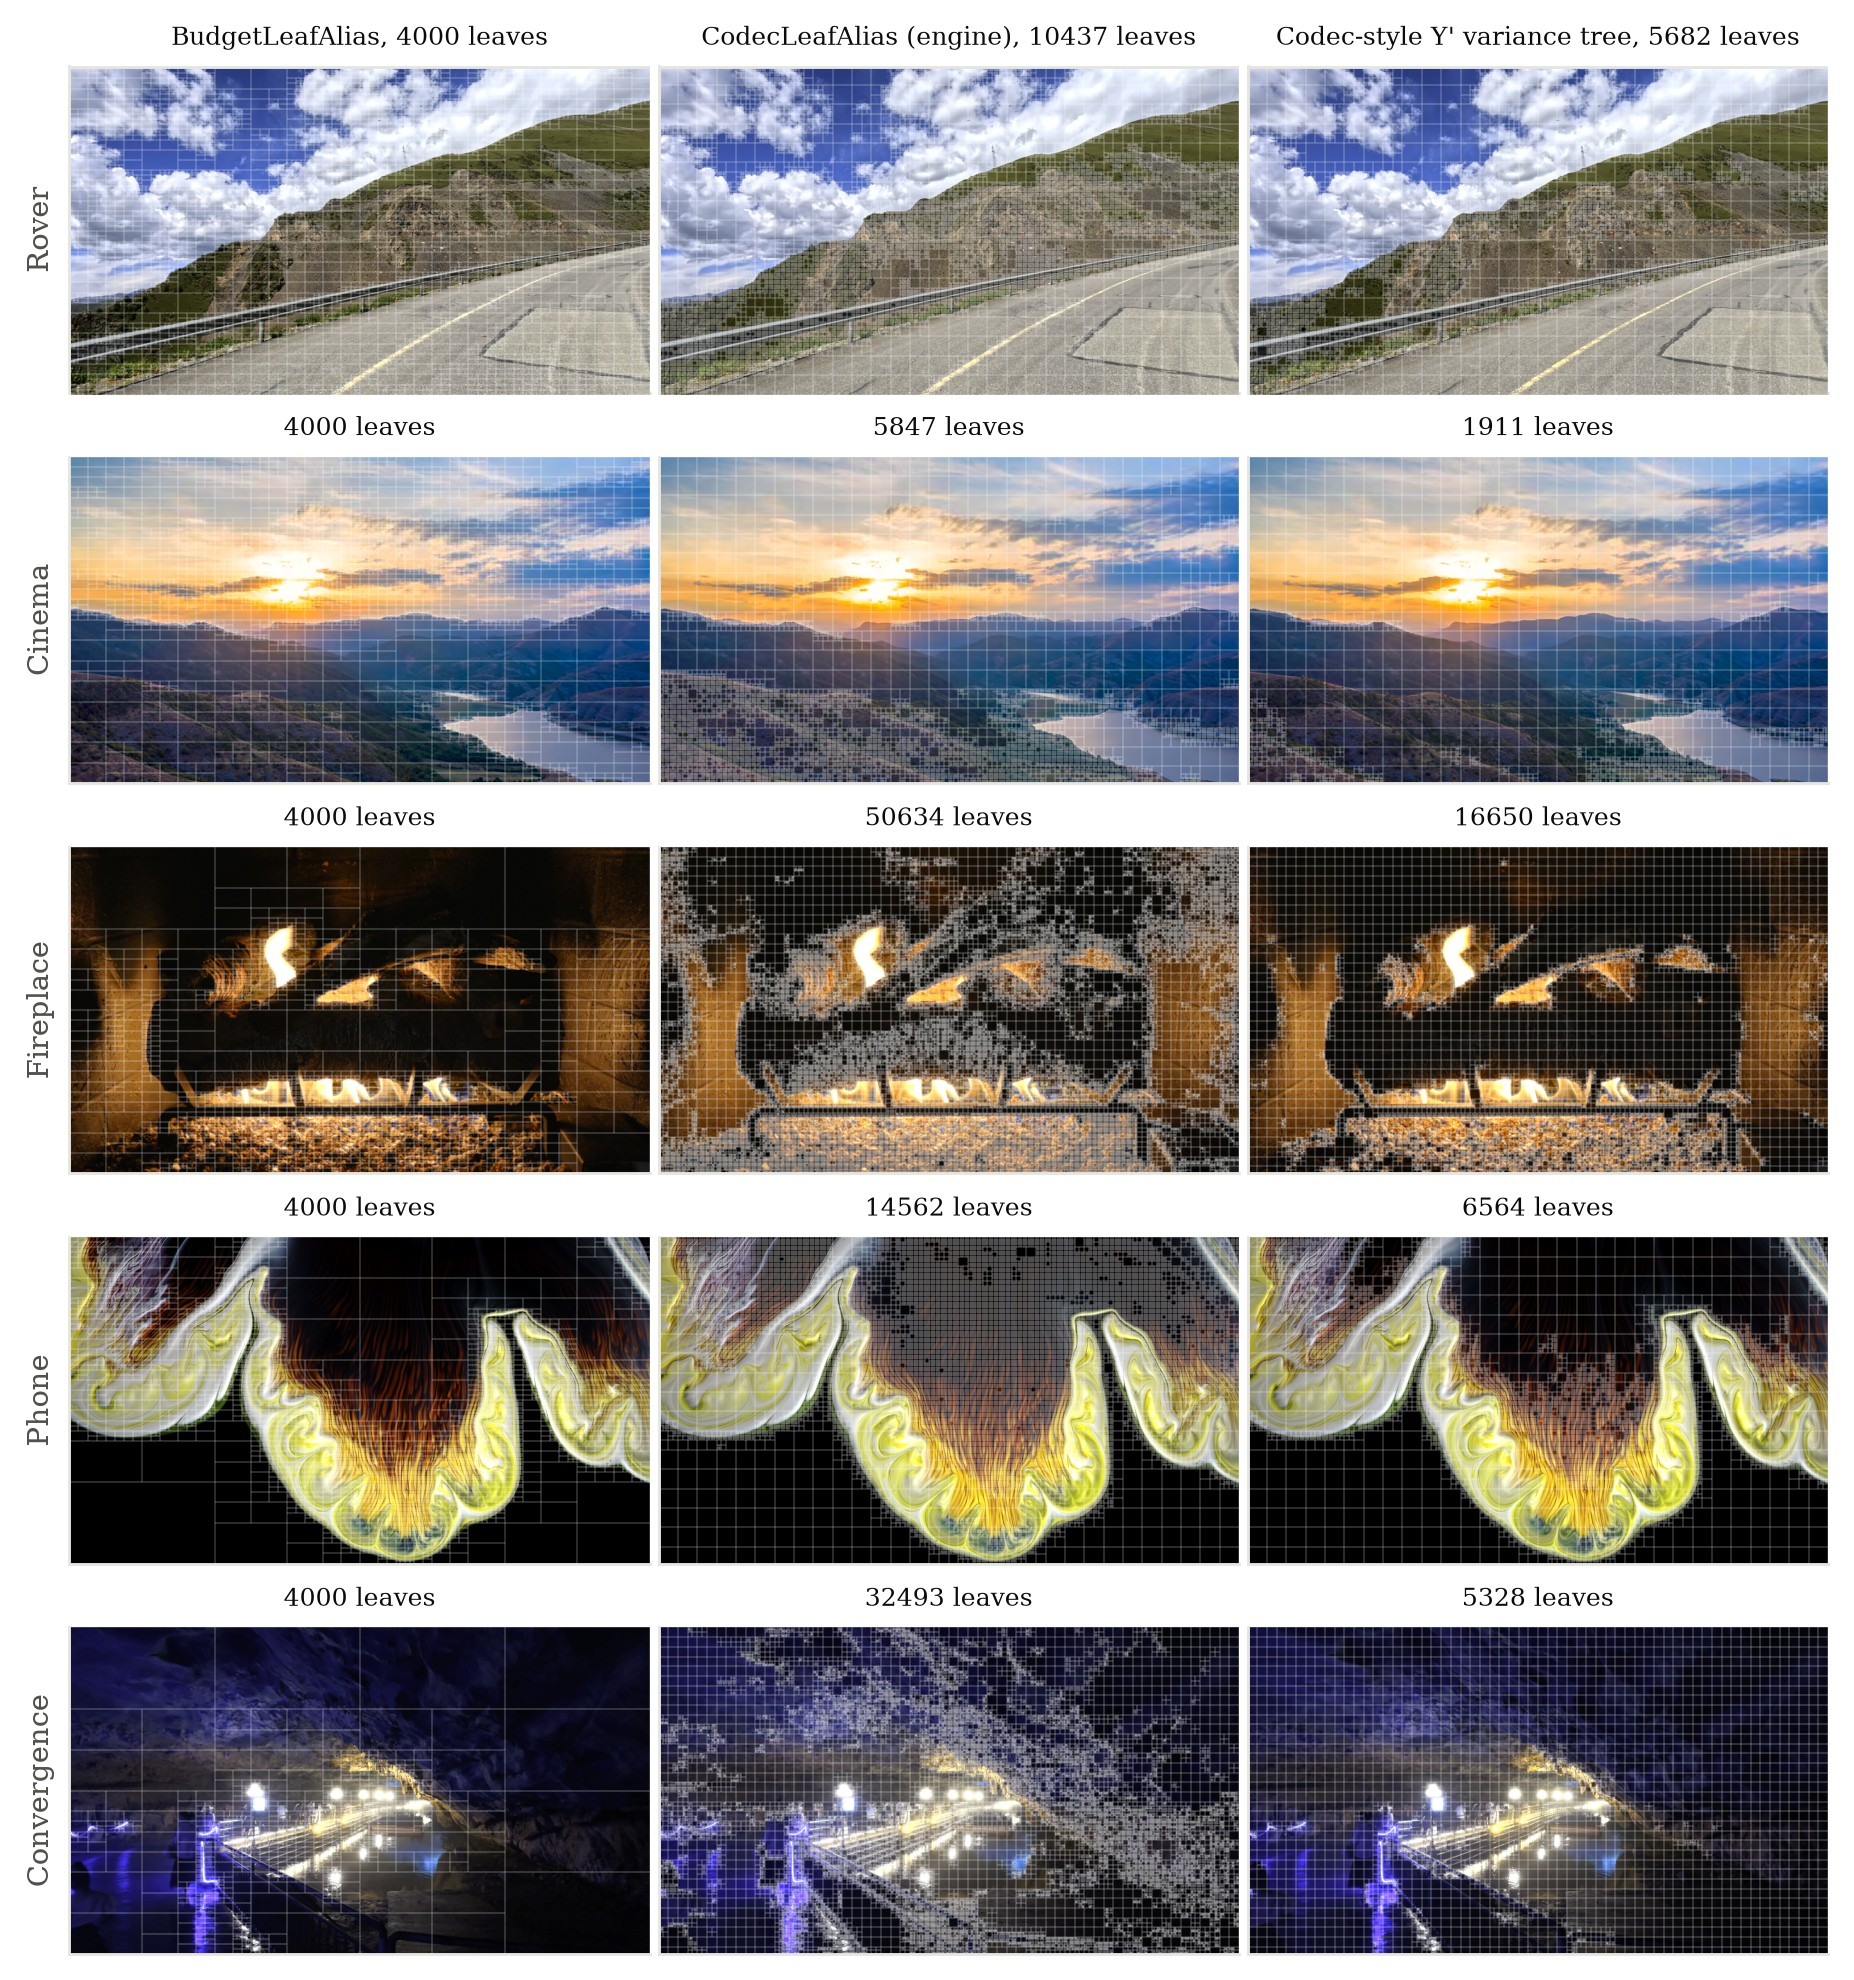
\includegraphics[width=\columnwidth]{fig_partitions.jpg}
  \caption{\newmat Leaf partitions of one frame of Rover and Phone. .}
  \label{fig:partitions}
\end{figure}

Figure~\ref{fig:variance} shows variance against leaf count for BudgetLeafAlias at varying number of leaves, and CodecLeafAlias. 
The plots show that codec leaves are placed less usefully for light sampling in every scene the codec partition lies above the budget curve, and BudgetLeafAlias reaches the same variance with 23--54\% of its leaves (94\% in Phone). A codec partition helps when it has considerably more leaves than the budget: in Fireplace Room it has about 47000 leaves, 12 times the budget, and reaches 0.26 of its variance; in Convergence about 27000 and 0.48. Rendered at equal samples, CodecLeafAlias is accordingly 5.3\% better than BudgetLeafAlias in Fireplace Room and 1.7\% better in Convergence (Figure~\ref{fig:equalsamples}), and it has the best full-video result on those two scenes (Table~\ref{tab:main}). 

\begin{figure}[htbp!]
  \centering
  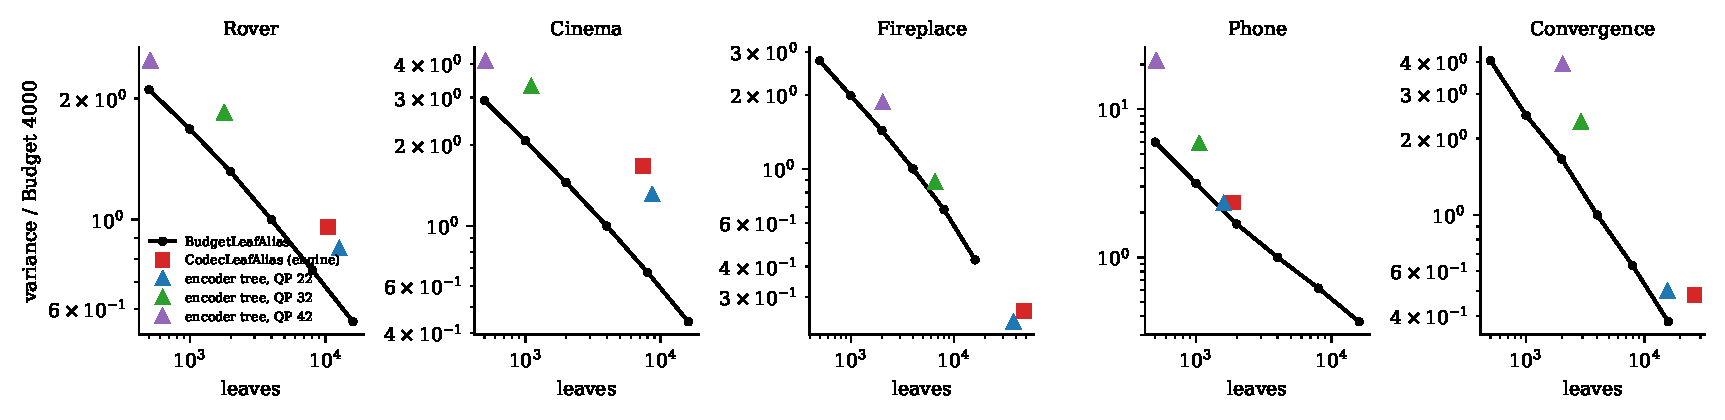
\includegraphics[width=\columnwidth]{fig_variance_vs_leaves.pdf}
  \caption{\newmat Light-sampling variance against leaf count, relative to BudgetLeafAlias with 4000 leaves (median over frames). Each line is BudgetLeafAlias from 500 to 16000 leaves in one scene, and the square of the same color is the CodecLeafAlias partition of that scene. }
  \label{fig:variance}
\end{figure}

A codec partition fails in two situations. On dark or low-contrast content the leaves go to dark detail: the Cinema partition has 7400 leaves and still 1.67 times the variance of 4000 budget leaves. And the leaf count swings with the content, by 40 times within the Phone video (528 to 20133), and with it the memory (0.2 to 2.2\,MB per frame) and the sampling cost, against a fixed 75\,KB. In summary, CodecLeafAlias is preferable when a decoded stream is at hand, the light is concentrated or the content bright and detailed, and a variable memory footprint is acceptable. BudgetLeafAlias is preferable when memory or cache size must be bounded, on dark or fading content, whenever predictable cost matters, and for emissive textures that are not decoded from a stream at all (rendered, procedural or uncompressed). The two can be combined by merging a codec partition down to a budget with the same $\mathrm{Var}\cdot A$ rule. 

\paragraph{Quantization and bitrate.}
As discussed in Section~\ref{sec:codec}, compression does not introduce bias to the estimate, so the question is how much variance it adds. We encoded the five videos in 10-bit PQ with libvpx-vp9 (CRF 12, 32, 48, 63), x265 (CRF 18, 28, 40) and SVT-AV1 (CRF 25, 40, 55), from 74 down to 0.6\,Mb/s (decoded PSNR from 51 to 32\,dB), took the leaf weights from the decoded planes as described in Section~\ref{sec:codec}, and rendered one inter-coded frame per scene at equal samples (32 captures) against the same partition with exact leaf weights.

Every ratio lies between 0.995 and 1.029 (Figure~\ref{fig:rate}), the largest PSNR loss is 0.23\,dB, and the ratios do not grow as the bitrate falls: compression error is spread over each block, while a leaf weight is the mean over the whole leaf, so most of it averages out. Taking the partition from the decoded frame instead of the source gives 0.996--1.019. Quantizing the block means directly isolates the effect of the DC quantizer: up to a step of 64 of the 1023 code values the error grows by about 3\% at most, for both partitions, and only a step of 256, a quarter of the range, reaches 4--13\%. Using the luma mean alone instead of the three planes changes the error by at most 1.5\%. 

\begin{figure}[htbp!]
  \centering
  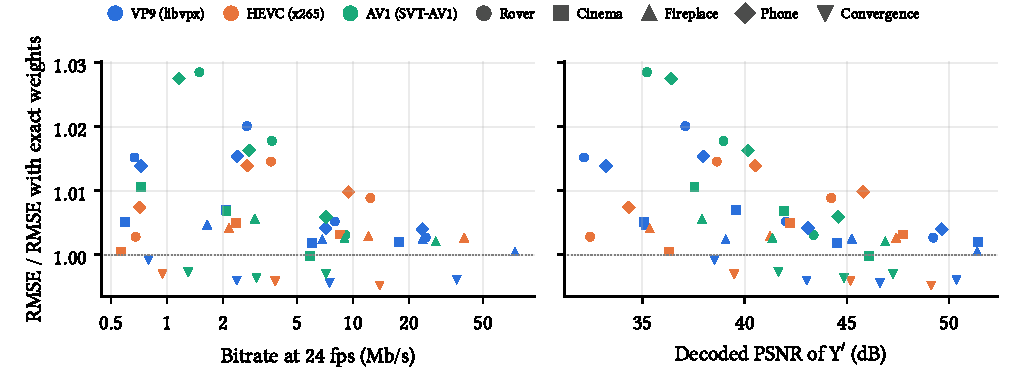
\includegraphics[width=\columnwidth]{fig_rate_sensitivity.pdf}
  \caption{\newmat RMSE of the rendered frame with leaf weights taken from lossy encodes, relative to exact leaf weights, against bitrate (left) and decoded PSNR (right), for three codecs and five scenes. All 50 points lie between 0.995 and 1.029, with no trend toward low bitrates.}
  \label{fig:rate}
\end{figure}

\paragraph{Other codecs and encoder settings.}
CodecLeafAlias needs two things from a codec: a block partition that follows image content, and the mean of each block. Every block-based codec provides the second; the first depends on the frame type. A standard configuration chooses blocks by rate-distortion (RD) search. In an intra-coded frame this splits where the image is detailed, which is what the sampler needs. In a predicted frame the search runs on the residual left after motion compensation, so its blocks follow prediction error rather than content: where motion is predicted well, a detailed region can be coded as one large block (Figure~\ref{fig:trees}).

\begin{figure}[htbp!]
  \centering
  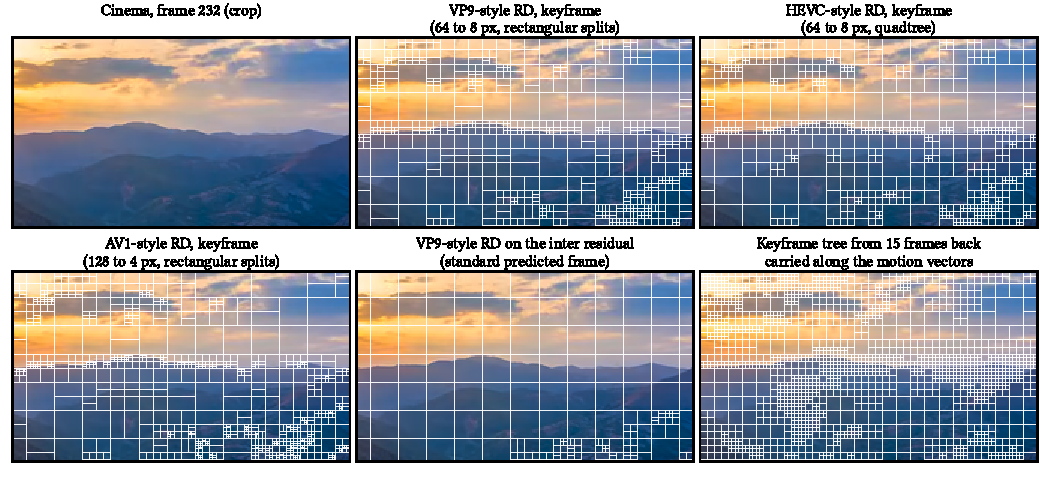
\includegraphics[width=\columnwidth]{fig_codec_trees.pdf}
  \caption{\newmat Partitions of a Cinema frame at quantizer 64 of 1023. Keyframe RD trees of the three codec families follow content. The RD tree of a predicted frame (bottom middle) follows prediction error instead and leaves most of the details in large blocks. The keyframe tree carried along the motion vectors (bottom right) follows content again.}
  \label{fig:trees}
\end{figure}

We reproduced the partition search of the three codec families on our frames, with their block sizes and split modes (VP9 and HEVC from 64 to 8 pixels, AV1 from 128 to 4), at quantizers 16, 64 and 256 of 1023, and rendered each partition with exact leaf means at equal samples. Used directly, the RD tree of a predicted frame costs up to 12\% for VP9 and HEVC and 22\% for AV1 at quantizer 64, relative to the CodecLeafAlias partition. Reusing the last keyframe's tree without moving it is better but drifts as the content moves (up to 6\%). Carrying the keyframe tree along the motion vectors of the stream, the strategy proposed in Section~\ref{sec:codec}, solves both: it stays within 2.5--4.2\% of the CodecLeafAlias partition at quantizers 16 and 64 for all three codec families, and within 5.4--6.6\% at quantizer 256, which is comparable to a partition built without any codec data. The three families behave alike for every partition source, and with weights from real encodes their worst ratios are 1.020 (VP9), 1.015 (HEVC) and 1.029 (AV1). The method is therefore tied neither to VP9 nor to its variance partitioning mode. 
\newend

\subsection{Denoised Results}
\label{sec:denoise}
Real-time renders are frequently paired with a neural denoiser in production. We pass each
technique's calibrated real-time render through the same OptiX denoiser~\cite{nvidia2021optixdenoiser} and re-measure
RMSE against the reference. Table~\ref{tab:denoise} shows that on every scene tested,
starting from our lower-noise image lets the denoiser reach a lower final RMSE than starting
from Random or 2D CDF.

\begin{table}[htbp!]
\centering
\small
\caption{RMSE before and after denoising. On every scene tested, whichever of our two techniques wins that scene keeps the lowest denoised RMSE too. }
\label{tab:denoise}
\begin{tabular}{ll cc}
\toprule
Scene & Technique & Noisy RMSE & Denoised RMSE \\
\midrule
\multirow{3}{*}{Rover}
 & Random & 0.0468 & 0.0381 \\
 & 2D CDF & 0.0779 & 0.0424 \\
 & {BudgetLeafAlias} & \textbf{0.0367} & \textbf{0.0375} \\
\midrule
\multirow{3}{*}{Cinema}
 & Random & 0.1109 & 0.0111 \\
 & 2D CDF & 0.1218 & 0.0110 \\
 & {CodecLeafAlias} & \textbf{0.0933} & \textbf{0.0106} \\
\midrule
\multirow{3}{*}{Fireplace Room}
 & Random & 0.5516 & 0.0312 \\
 & 2D CDF & 0.2295 & 0.0233 \\
 & {CodecLeafAlias} & \textbf{0.2087} & \textbf{0.0225} \\
\midrule
\multirow{3}{*}{Convergence}
 & Random & 0.3296 & 0.0148 \\
 & 2D CDF & 0.1428 & 0.0041 \\
 & {CodecLeafAlias} & \textbf{0.0870} & \textbf{0.0034} \\
\bottomrule
\end{tabular}
\end{table}


Convergence benefits the most: denoising cuts RMSE by over $95\,\%$ for every technique, and
CodecLeafAlias still finishes with the lowest denoised RMSE of the three ($0.0034$,
against $0.0041$ for 2D CDF), a direct result of feeding the denoiser a cleaner starting
image. Figure~\ref{fig:denoisedflip} additionally shows
denoised closeups and their \FLIP\  error maps for Convergence and Fireplace Room. 2D CDF's denoised output keeps a visibly brighter (higher-error) \FLIP\ map.

\new{The differences between techniques are nevertheless much smaller after denoising than before it, for two reasons. First, the denoiser removes mostly the high-frequency, per-pixel part of the error, which is precisely where light samplers differ; what remains is dominated by low-frequency residue that depends little on the number of light samples. Second, as discussed in Section~\ref{sec:equalquality}, light sampling is only one term of the error of a frame, so the room for any emission sampler is bounded before the denoiser acts. For a denoised pipeline the practical reading is the one of Section~\ref{sec:equalquality}: similar final quality is obtained from a sampler that costs less time and memory.}

Figure~\ref{fig:teaser} shows full-frame comparisons and closeups for Rover and Cinema, where
BudgetLeafAlias and CodecLeafAlias respectively remove most of the speckled noise still
visible in Random and 2D CDF's closeups. Figure~\ref{fig:figuresonly} shows
the same treatment for the remaining three scenes against a converged reference, with two matched closeups per scene; each panel also shows, in its top-left
corner, the actual HDR emissive texture that lit that scene. CodecLeafAlias visibly reduces
noise relative to both baselines.

\begin{figure*}[htbp!]
  \centering
  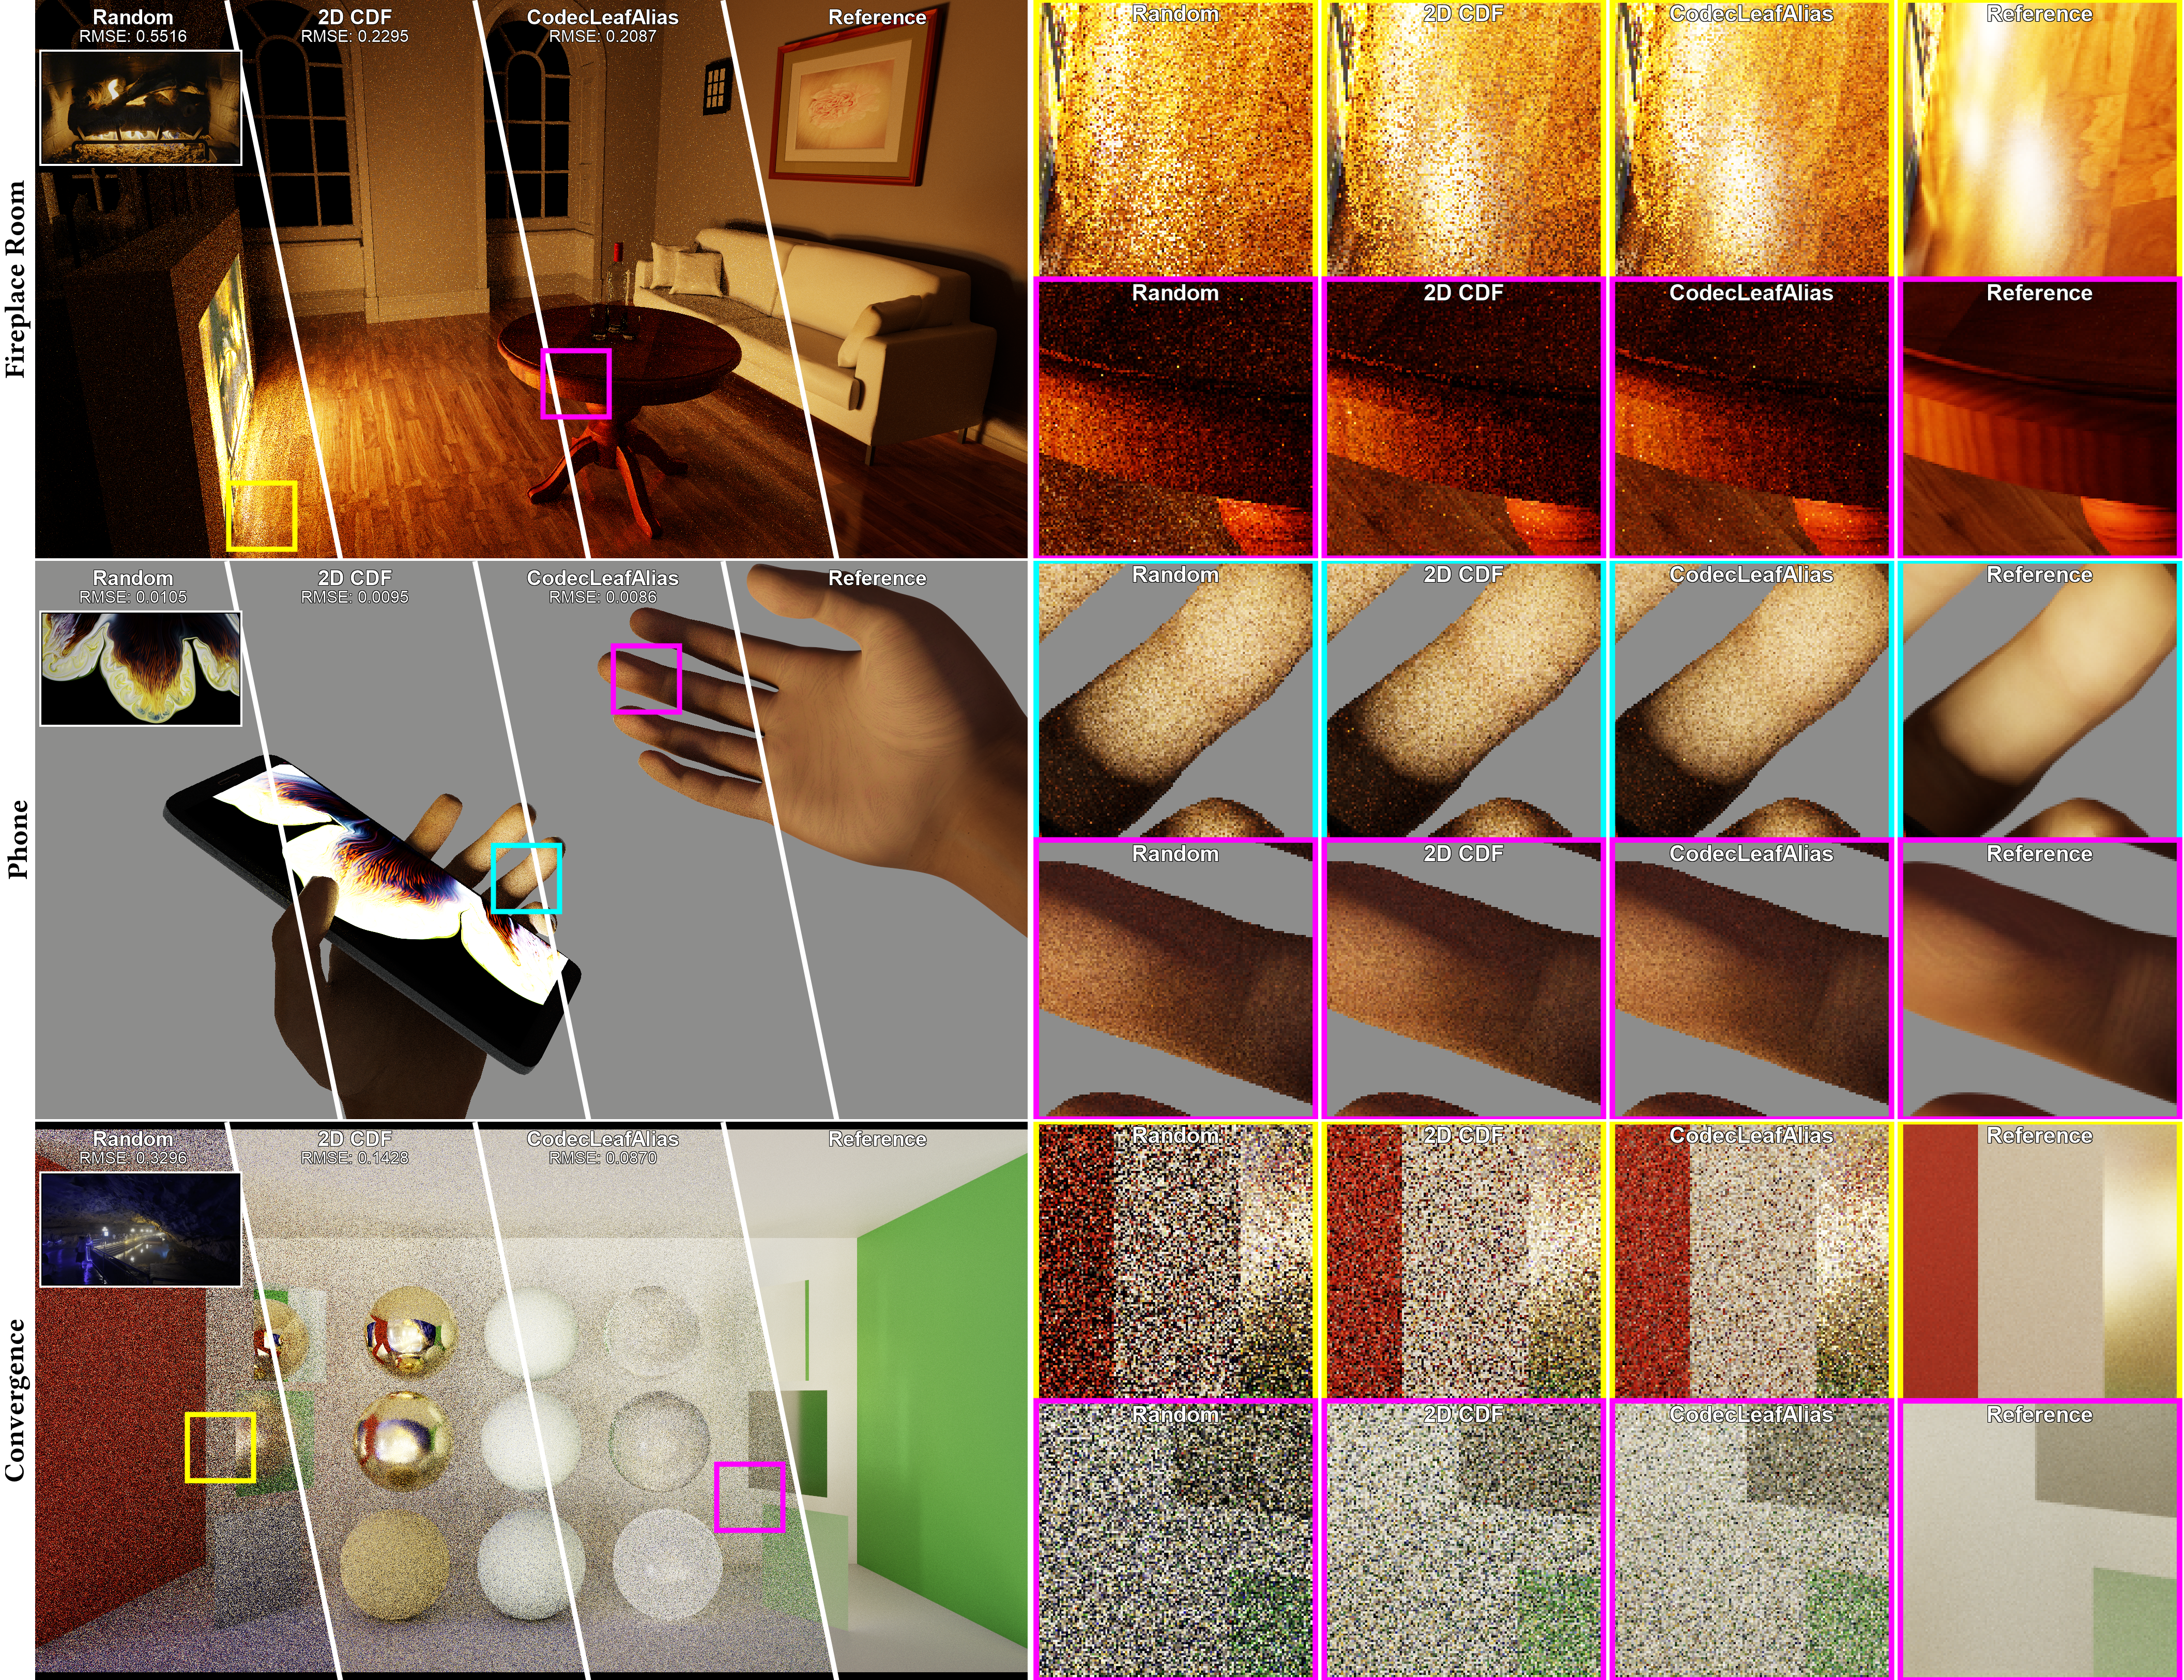
\includegraphics[width=\textwidth]{figures_only_restir_v9.png}
  \caption{Fireplace Room, Phone, and Convergence: full-frame diagonal comparisons
  (Random / 2D CDF / CodecLeafAlias / Reference) with real measured RMSE per technique, two
  large matched closeups per scene, and each scene's emissive HDR texture (top-left inset). }
  \label{fig:figuresonly}
\end{figure*}

\begin{figure*}[htbp!]
  \centering
  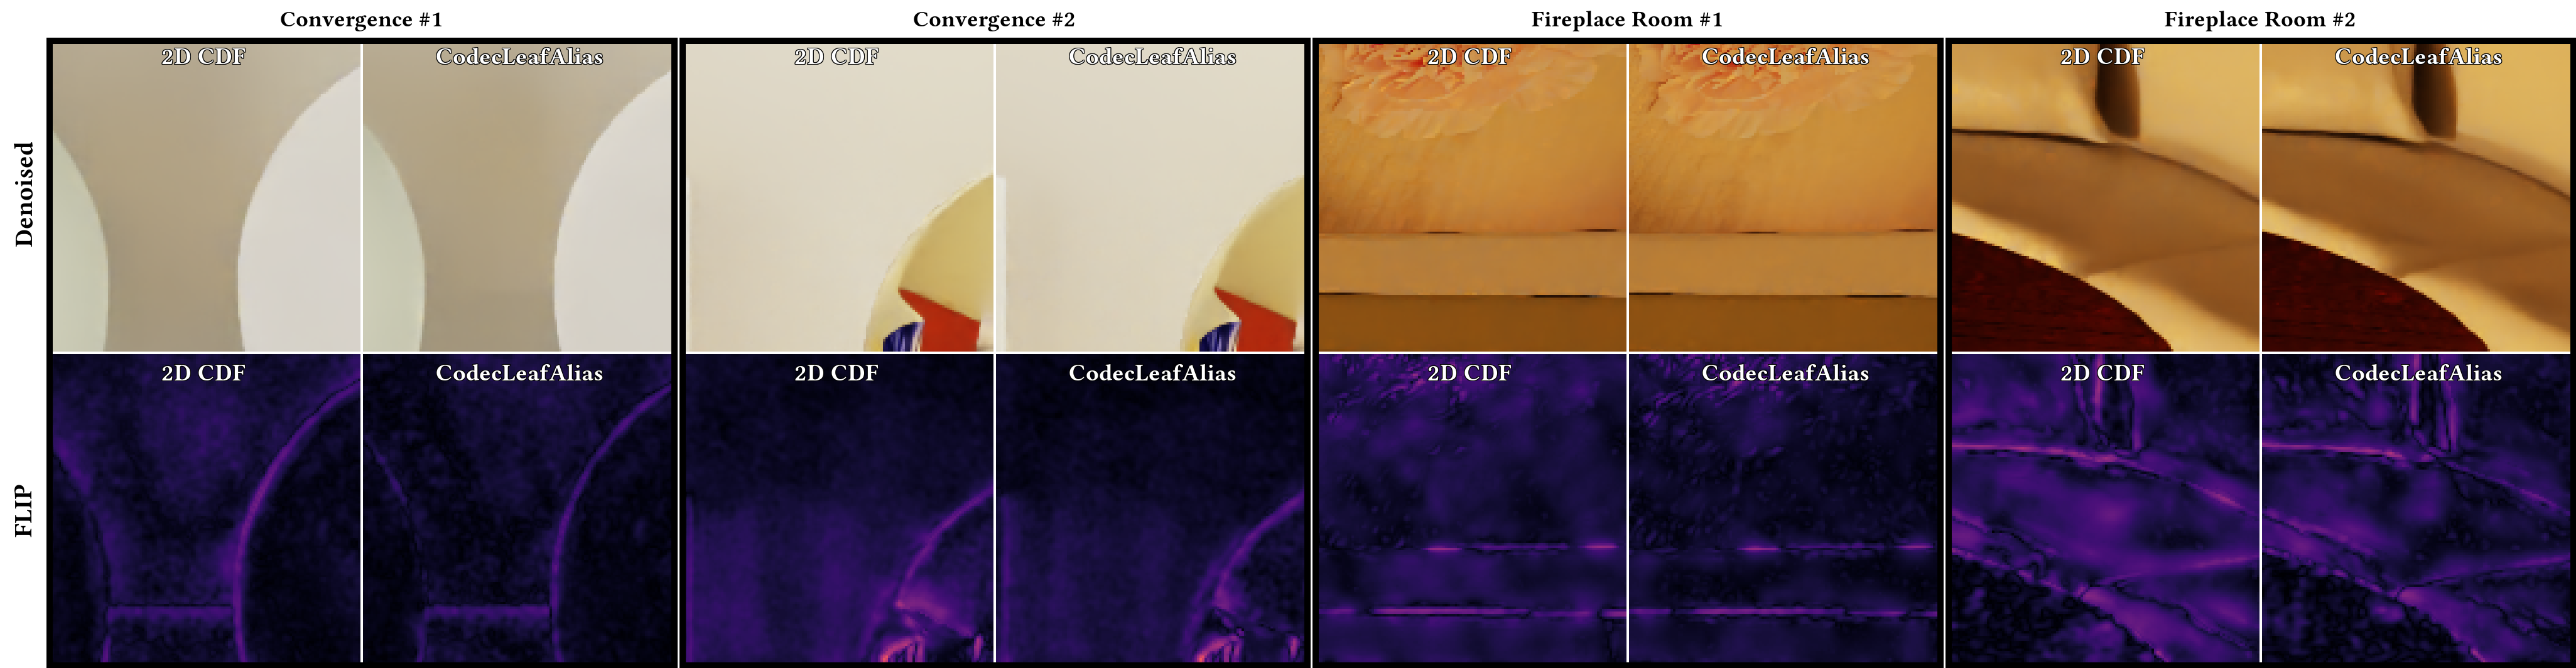
\includegraphics[width=\textwidth]{denoised_flip_grid.png}
  \caption{Denoised closeups and FLIP error maps when compared to the reference, for 2D CDF
  and CodecLeafAlias, at the two regions per scene with the largest denoised FLIP gap, for
  Convergence and Fireplace Room.}
  \label{fig:denoisedflip}
\end{figure*}

\subsection{\texorpdfstring{\newt{Discussion and limitations}}{Discussion and limitations}}
\label{sec:limits}

\newbegin
LeafAlias helps most when the sampling structure has to be small and cheap: several video lights at once, high-resolution emitters, limited memory or upload bandwidth, a tight frame, and scenes where the light sampler accounts for a large part of the error. Its limits follow from the same measurements. (i)~At equal samples it is never better than a per-texel distribution; a larger leaf budget reduces the loss. (ii)~Its gain comes from fitting more light samples in the frame, so it disappears when light sampling is a small part of the frame's cost or of its error. (iii)~It considers the texture alone: the BSDF, visibility and the distance to the emitter contribute variance that no scene-independent emission sampler removes, which bounds the gain of any such sampler. (iv)~The alias mapping does not exploit low-discrepancy sample sequences (Appendix~\ref{app:qmc}); a monotone mapping such as a 2D CDF does. (v)~Our implementation stores the mean luminance of a leaf as a 16-bit float, which saturates at 65504; emitters with brighter texels may need a wider format. (vi)~Extracting the partitions from the encoded metadata might pose some difficulty in video workflows involving hardware-accelerated decoding pipelines..
\newend

\section{Conclusions and future work} \label{sec:conclusions}

We introduced LeafAlias, a family of samplers for dynamic emissive textures that build a per-frame alias table over a variance-driven quadtree rather than over raw pixels. \rev{The outcome is a sampler that is inexpensive enough to rebuild in every frame, small enough to stay resident in the GPU's L1 cache, and accurate enough to stay within a few percent of the per-texel methods we compared against at equal samples, while reaching their quality up to 3 times faster.}

\rev{The consistency of CodecLeafAlias results through the different video light sources, codecs and bitrates that were tested suggests that the coded signal carries enough information to be reused for importance sampling. The advantage holds up when quality is judged over a full animated sequence rather than a single frame, and narrows, as for any light sampler, once a denoiser is added to the pipeline.} We also show that, when not available, building a small variance-driven quadtree is fast and can improve performance. The decision to use more or fewer leaves depends on the scene complexity and video material.

More broadly, this work points to an under-exploited overlap between the toolchains of video compression and real-time rendering. We think this connection has more to offer than the single, frame-local piece of it used here. The most direct extension is temporal. The coding-tree partition is currently extracted in every frame, discarding the motion vectors the same encoder already computes to relate consecutive frames. Since those vectors describe how the variance structure itself is moving, they could warp the previous frame's leaves into a predicted partition for the current one.
A second direction targets the leaf weights rather than the partition. CodecLeafAlias currently estimates each leaf's radiance from a single DC coefficient, which is exact under a piecewise-constant model but discards the higher-frequency information. That information could be used to guide the sampling within the leaf rectangle, potentially improving the efficiency of each drawn sample. \new{A third is the mapping itself: a hierarchical warp~\cite{clarberg2005wavelet} down the same quadtree keeps the leaf density and its small footprint, and could recover the benefit of low-discrepancy sequences that the alias mapping gives up (Appendix~\ref{app:qmc}).}

Finally, because every LeafAlias sample already carries an unbiased pdf, it composes naturally with spatiotemporal resampling: using it purely as the candidate generator inside a ReSTIR-style reservoir, rather than as the final sampler, may provide additional variance reduction on scenes with several bright, moving regions competing for the light budget.

\bibliographystyle{ACM-Reference-Format}
\bibliography{sample-base}

\appendix

\section{\texorpdfstring{\newt{Per-pixel alias tables and low-discrepancy input}}{Per-pixel alias tables and low-discrepancy input}}
\label{app:qmc}

\newbegin
The results of the paper use independent random numbers. Renderers driven by quasi-Monte Carlo (QMC) sequences expose a further difference between a per-pixel alias table and a table over leaves, which we document here. The claim is limited: LeafAlias does \emph{not} exploit low-discrepancy input; it avoids a failure of per-pixel alias tables under such input. Since the Fourier spectrum of a non-uniform sample set is not a measure of its discrepancy under the target density~\cite{li2026gradient}, we do not rely on spectra, and measure the integration error of rendered images instead.

\paragraph{How the pattern arises.}
A per-pixel alias table maps a sample $(u,v)$ to bucket $k=\lfloor un\rfloor$ of $n$ (one per texel), keeps the bucket's own texel if $v<\tau_k$ and otherwise jumps to its alias. The $N$ values of $u$ that a pixel draws from a low-discrepancy sequence are spread almost evenly over $[0,1)$, so they visit the table at a nearly constant stride of $n/N$ buckets. Vose's construction, as implemented in our renderer, lists below-mean and above-mean texels in scan order and pairs them in that order, so inside any region whose texels are all on the same side of the mean (a smooth sky, a dark hillside) consecutive buckets own consecutive texels. The constant stride through the table becomes a constant stride through the image, $H/N$ rows for an image of height $H$: when $N$ divides $H$, every sample of a pixel that falls in such a region lands in the same column. Figure~\ref{fig:qmcpoints} shows it on a $1024{\times}512$ region of the Cinema texture: the 2D CDF keeps the even spread of the Halton input, while the per-pixel alias table stacks the samples of the hillside into lines. In the spectrum of 60000 points, the strongest line is 41 times its median for the per-pixel alias table, against 1.4 for the 2D CDF and for BudgetLeafAlias. Two conditions must hold together: a stride aligned with the image rows, and long scan-order runs in the table. A textbook construction that keeps scan order everywhere, as in Figure~\ref{fig:spectrum}, produces a lattice over the whole image. Owen-scrambled sequences~\cite{owen1995randomly} randomize the stride and, in our test, remove most of the effect.

\begin{figure}[htbp!]
  \centering
  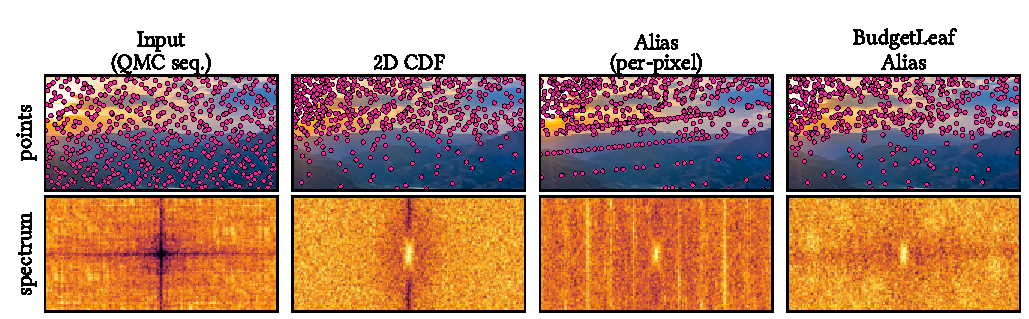
\includegraphics[width=\columnwidth]{fig_qmc_points.pdf}
  \caption{\newmat Top: the first 500 points of the Halton sequence (bases 2, 3), as input and after each warp, over a $1024{\times}512$ region of the Cinema texture. Bottom: power spectrum of the first 60000 points. The per-pixel alias table uses the table construction of our renderer; BudgetLeafAlias uses 4000 leaves.}
  \label{fig:qmcpoints}
\end{figure}

\paragraph{What it costs in a rendering.}
We render a diffuse floor lit by the textured area light through a fence (direct lighting, light sampling only, no MIS), with the Halton set and an independent toroidal shift per pixel, against an exact reference obtained by quadrature over the emitter (Figure~\ref{fig:qmcfence}, Table~\ref{tab:qmc}). With pseudorandom numbers the samplers are equal, as their densities predict. With QMC input the 2D CDF becomes 3.5 times better and the per-pixel alias table 2.6 times \emph{worse}, while LeafAlias stays at its pseudorandom level. The per-pixel alias table with QMC does not converge at all between 128 and 512 samples per pixel, where the stride is 4, 2 and 1 rows (relative RMSE 0.145 and 0.143 on the unoccluded part of the floor, against 0.054 and 0.025 for LeafAlias and 0.013 and 0.004 for the 2D CDF), and starts to fall only at 1024 samples.

\begin{figure}[htbp!]
  \centering
  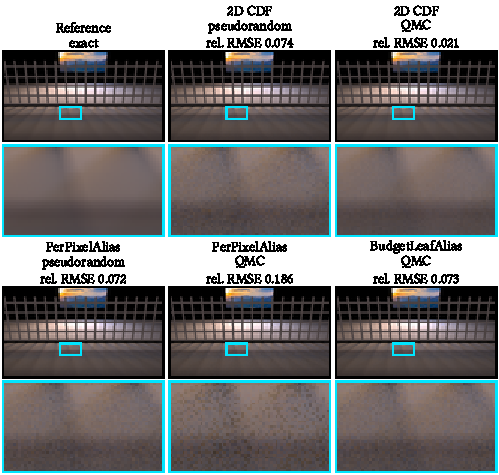
\includegraphics[width=0.92\columnwidth]{fig_qmc_fence.pdf}
  \caption{\newmat A diffuse floor lit through a fence by the emitter of Figure~\ref{fig:qmcpoints}, at 128 samples per pixel: exact reference; 2D CDF with pseudorandom and QMC input; per-pixel alias table with pseudorandom and QMC input; BudgetLeafAlias with QMC input. Close-ups below each render.}
  \label{fig:qmcfence}
\end{figure}

\begin{table}[htbp!]
\centering\small\newmat
\caption{\newmat Top: relative RMSE of the scene of Figure~\ref{fig:qmcfence} at 128 samples per pixel. Bottom: ratio of the QMC error to the sampler's own pseudorandom error over 2406 emitters and emitter regions (photographs, video frames, sky images and windows of our textures), one shading point behind six kinds of occluder.}
\label{tab:qmc}
\begin{tabular}{lcc}
\toprule
Relative RMSE, 128 spp & Pseudorandom & QMC \\
\midrule
2D CDF & 0.074 & 0.021 \\
Per-pixel Alias & 0.072 & 0.186 \\
BudgetLeafAlias (4000 leaves) & 0.074 & 0.073 \\
LeafAlias (1000 leaves) & 0.075 & 0.072 \\
\midrule
QMC error / own pseudorandom & 128 spp & 1024 spp \\
\midrule
Per-pixel Alias, median & 0.92 & 0.79 \\
\quad cases above 1.10 & 16.7\% & 7.3\% \\
\quad worst case & 1.85 & 3.51 \\
BudgetLeafAlias, median & 0.99 & 0.93 \\
\quad cases above 1.10 & 0.0\% & 0.5\% \\
\quad worst case & 1.10 & 1.20 \\
\bottomrule
\end{tabular}
\end{table}

This is not a property of one region: of 225 overlapping $1024{\times}512$ windows of the same frame, the per-pixel alias table with QMC is worse than with pseudorandom numbers in 131, and it is worse in 65\% of the 40 flat sky photographs we tested. Over 2406 emitters (Table~\ref{tab:qmc}, bottom), the QMC error of BudgetLeafAlias stays within 10\% of its own pseudorandom error in more than 99\% of the cases, whereas the per-pixel alias table exceeds that bound in 7--17\% of the cases and reaches 3.5 times. These magnitudes are a best case for QMC, a single two-dimensional direct-lighting integral; in a full path tracer both the gain of the 2D CDF and the loss of the per-pixel alias table are smaller.

\paragraph{Scope.}
A table over a few thousand leaves, each covering many texels, has no fixed relation between bucket stride and image position, so it creates no pattern; but it does not preserve the low-discrepancy distribution either, and its QMC and pseudorandom errors are the same. The 2D CDF and hierarchical warps do preserve it, at the memory and per-sample cost reported in Section~\ref{sec:cost}, and the 2D CDF remains the lowest-error sampler under QMC when that cost is not a concern. On emitters that do not trigger the pattern, among them the five videos of this paper, the per-pixel alias table with QMC input had lower error than LeafAlias. The advantage of LeafAlias here is predictability: its error does not depend on whether the pattern conditions are met. The \supp{qmc\_note}, with its code, reproduces these figures and tables and adds a convergence study.
\newend

\section{\texorpdfstring{\newt{Temporal stability}}{Temporal stability}}
\label{app:temporal}

\newbegin
We evaluate temporal stability on 60 consecutive frames of each scene, rendered at equal samples with a new random seed every frame, against a converged reference for every frame. With $I_t$ the render and $R_t$ the reference of frame $t$, the \emph{temporal error} is
\begin{equation}
E_T = \sqrt{\left\langle\left[(I_t - I_{t-1}) - (R_t - R_{t-1})\right]^2\right\rangle},
\end{equation}
averaged over pixels and frames: subtracting the reference's own change removes what the video itself does, so only change introduced by the renderer remains. The \emph{low-frequency temporal error} is the same quantity after a Gaussian blur with $\sigma = 8$ pixels, which averages out per-pixel noise and keeps the kind of change that is seen as flicker, regions pulsing or popping between frames. Independently of rendering, we measure how much the sampling density changes between consecutive frames with the Jensen--Shannon divergence.

\paragraph{The coarser density changes less.} A per-texel density follows every change of the video, including compression noise, grain and small moving details. A leaf density averages each region over many texels, so these small changes largely cancel, and a leaf boundary that moves between frames only reassigns probability between neighbouring leaves of similar radiance. The density of BudgetLeafAlias changes 5.4, 2.5, 2.5 and 1.8 times less than the exact one in Rover, Cinema, Phone and Convergence, and about the same in Fireplace Room (Figure~\ref{fig:temporal}, left), even though 3--13\% of the $8{\times}8$ cells change leaf size every frame.

\begin{figure}[t]
  \centering
  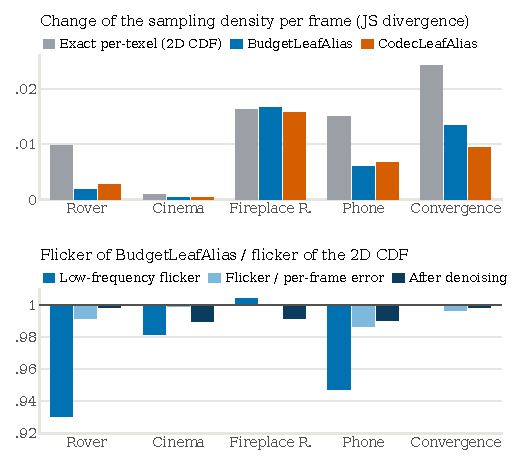
\includegraphics[width=\columnwidth]{fig_temporal.pdf}
  \caption{\newmat Top: change of the sampling density between consecutive frames, for the exact per-texel density (the 2D CDF's) and for the two LeafAlias densities. Bottom: rendered flicker of BudgetLeafAlias divided by the 2D CDF's, at equal samples; below 1 means less flicker.}
  \label{fig:temporal}
\end{figure}

\paragraph{Rendered flicker.} The low-frequency temporal error of BudgetLeafAlias is lower than the 2D CDF's in Rover, Cinema and Phone (7\%, 2\% and 5\% less) and the same in Fireplace Room and Convergence; that of CodecLeafAlias is within 0.0002 of the 2D CDF's in every scene (values of 0.0026--0.0072). The standard deviation over frames of the mean error of the whole frame (brightness pumping) is the same for all techniques. The full temporal error includes the per-pixel noise of each frame, so it grows with the per-frame error: BudgetLeafAlias is equal to or below the 2D CDF in Rover, Cinema and Phone and 4\% above it in Fireplace Room and Convergence, the two scenes where its per-frame RMSE is also 4--5\% higher. Divided by the per-frame RMSE, its temporal error is lower than the 2D CDF's in all five scenes: the partition changes add nothing measurable beyond the per-frame noise. After the OptiX denoiser, the temporal error of BudgetLeafAlias is equal to or lower than the 2D CDF's in every scene (Figure~\ref{fig:temporal}, right).

\paragraph{Frozen noise.} As a diagnostic, we also froze the random numbers (same seed every frame, no camera jitter), so that the image changes only through the video and the sampling structure. In that setting, where noise no longer hides it, the changing partition is visible as a fine-grained per-pixel change 1.5--3.6 times larger than the 2D CDF's, and a hierarchical warp over the same leaves brings it to 1.03--1.32 times. This setting does not occur in normal rendering, where a new seed every frame makes this change part of the per-frame noise, but it matters for techniques that reuse random numbers across frames, which we did not evaluate. The \supp{temporal\_stability} contains the complete tables.
\newend

\end{document}
"
\ifdefined\cleancopy\highlightfalse\fi
\ifhighlight
  \definecolor{newcolor}{RGB}{0,84,216}
  \definecolor{revcolor}{RGB}{226,106,0}
\else
  \definecolor{newcolor}{RGB}{0,0,0}
  \definecolor{revcolor}{RGB}{0,0,0}
\fi
\newcommand{\new}[1]{{\leavevmode\color{newcolor}#1}}
\newcommand{\rev}[1]{{\leavevmode\color{revcolor}#1}}
\newcommand{\newbegin}{\begingroup\color{newcolor}}
\newcommand{\newend}{\endgroup}
\newcommand{\newmat}{\color{newcolor}}
\newcommand{\revmat}{\color{revcolor}}
\DeclareRobustCommand{\newt}[1]{\textcolor{newcolor}{#1}}
\DeclareRobustCommand{\revt}[1]{\textcolor{revcolor}{#1}}
%% ---------------------------------------------------------------------------
%% Aspirational results (DRAFT ONLY): 
%%   \aspirational{text}            target text or value (magenta) followed by an [ASPIRATIONAL] tag
%%   \aspirational[note]{text}      same, with a note for whoever works on reaching the target
%%   \aspnote{note}                 the tag alone, for captions of tables and figures
%% Search this file and table_video_all.tex for "\asp" to list them.
%% ---------------------------------------------------------------------------
\definecolor{aspcolor}{RGB}{200,0,120}
\DeclareRobustCommand{\aspnote}[1]{{\leavevmode\color{aspcolor}\textsf{\bfseries[ASPIRATIONAL\if\relax\detokenize{#1}\relax\else: #1\fi]}}}
\newcommand{\aspirational}[2][]{{\leavevmode\color{aspcolor}#2}\,\aspnote{#1}}
%% Value inside a table cell: colour only, the note goes in the caption.
\newcommand{\aspcell}[1]{{\color{aspcolor}#1}}
%% Name of a document of the supplementary material.
\newcommand{\supp}[1]{supplementary document \texttt{#1}}

%%
%% The abstract is a short summary of the work to be presented in the
%% article.
\begin{abstract}
We present a method for fast importance sampling HDR textured lights that allows real-time video-driven lighting.
Our method partitions a light's texture into a budgeted, variance-driven quadtree and builds an alias table over the resulting leaves, avoiding the cost of a dense per-frame CDF while still capturing
the texture's overall energy distribution. We present two variants: one that reuses the per-frame hierarchical partitions already present in the metadata of modern video codecs, and another that builds a budgeted quadtree to fit the entire sampling structure in the L1 cache of the GPU. Compared to the dense 2D CDF-inversion baseline, at a matched real-time
frame-time budget our technique reduces RMSE by 9–53\% depending on
scene, by letting the saved sampling cost be reinvested in additional light
samples. \new{With the same number of samples, our technique doesn't introduce considerable error compared to 2D CDF, and delivers up to 3 times faster.}
It also reduces memory consumption and transfers by several orders of magnitude when compared to state-of-the-art samplers.

\end{abstract}

%%
%% The code below is generated by the tool at http://dl.acm.org/ccs.cfm.
%% Please copy and paste the code instead of the example below.
%%
\begin{CCSXML}
<ccs2012>
<concept>
<concept_id>10010147.10010371.10010382.10010385</concept_id>
<concept_desc>Computing methodologies~Image-based rendering</concept_desc>
<concept_significance>500</concept_significance>
</concept>
<concept>
<concept_id>10010147.10010371.10010395</concept_id>
<concept_desc>Computing methodologies~Image compression</concept_desc>
<concept_significance>500</concept_significance>
</concept>
<concept>
<concept_id>10010147.10010371.10010372.10010374</concept_id>
<concept_desc>Computing methodologies~Ray tracing</concept_desc>
<concept_significance>500</concept_significance>
</concept>
</ccs2012>
\end{CCSXML}

\ccsdesc[500]{Computing methodologies~Image-based rendering}
\ccsdesc[500]{Computing methodologies~Image compression}
\ccsdesc[500]{Computing methodologies~Ray tracing}

%%
%% Keywords. The author(s) should pick words that accurately describe
%% the work being presented. Separate the keywords with commas.
\keywords{Image-based lighting, video codecs, Alias tables, emissive textures, real-time rendering }

\begin{teaserfigure}
  \centering
  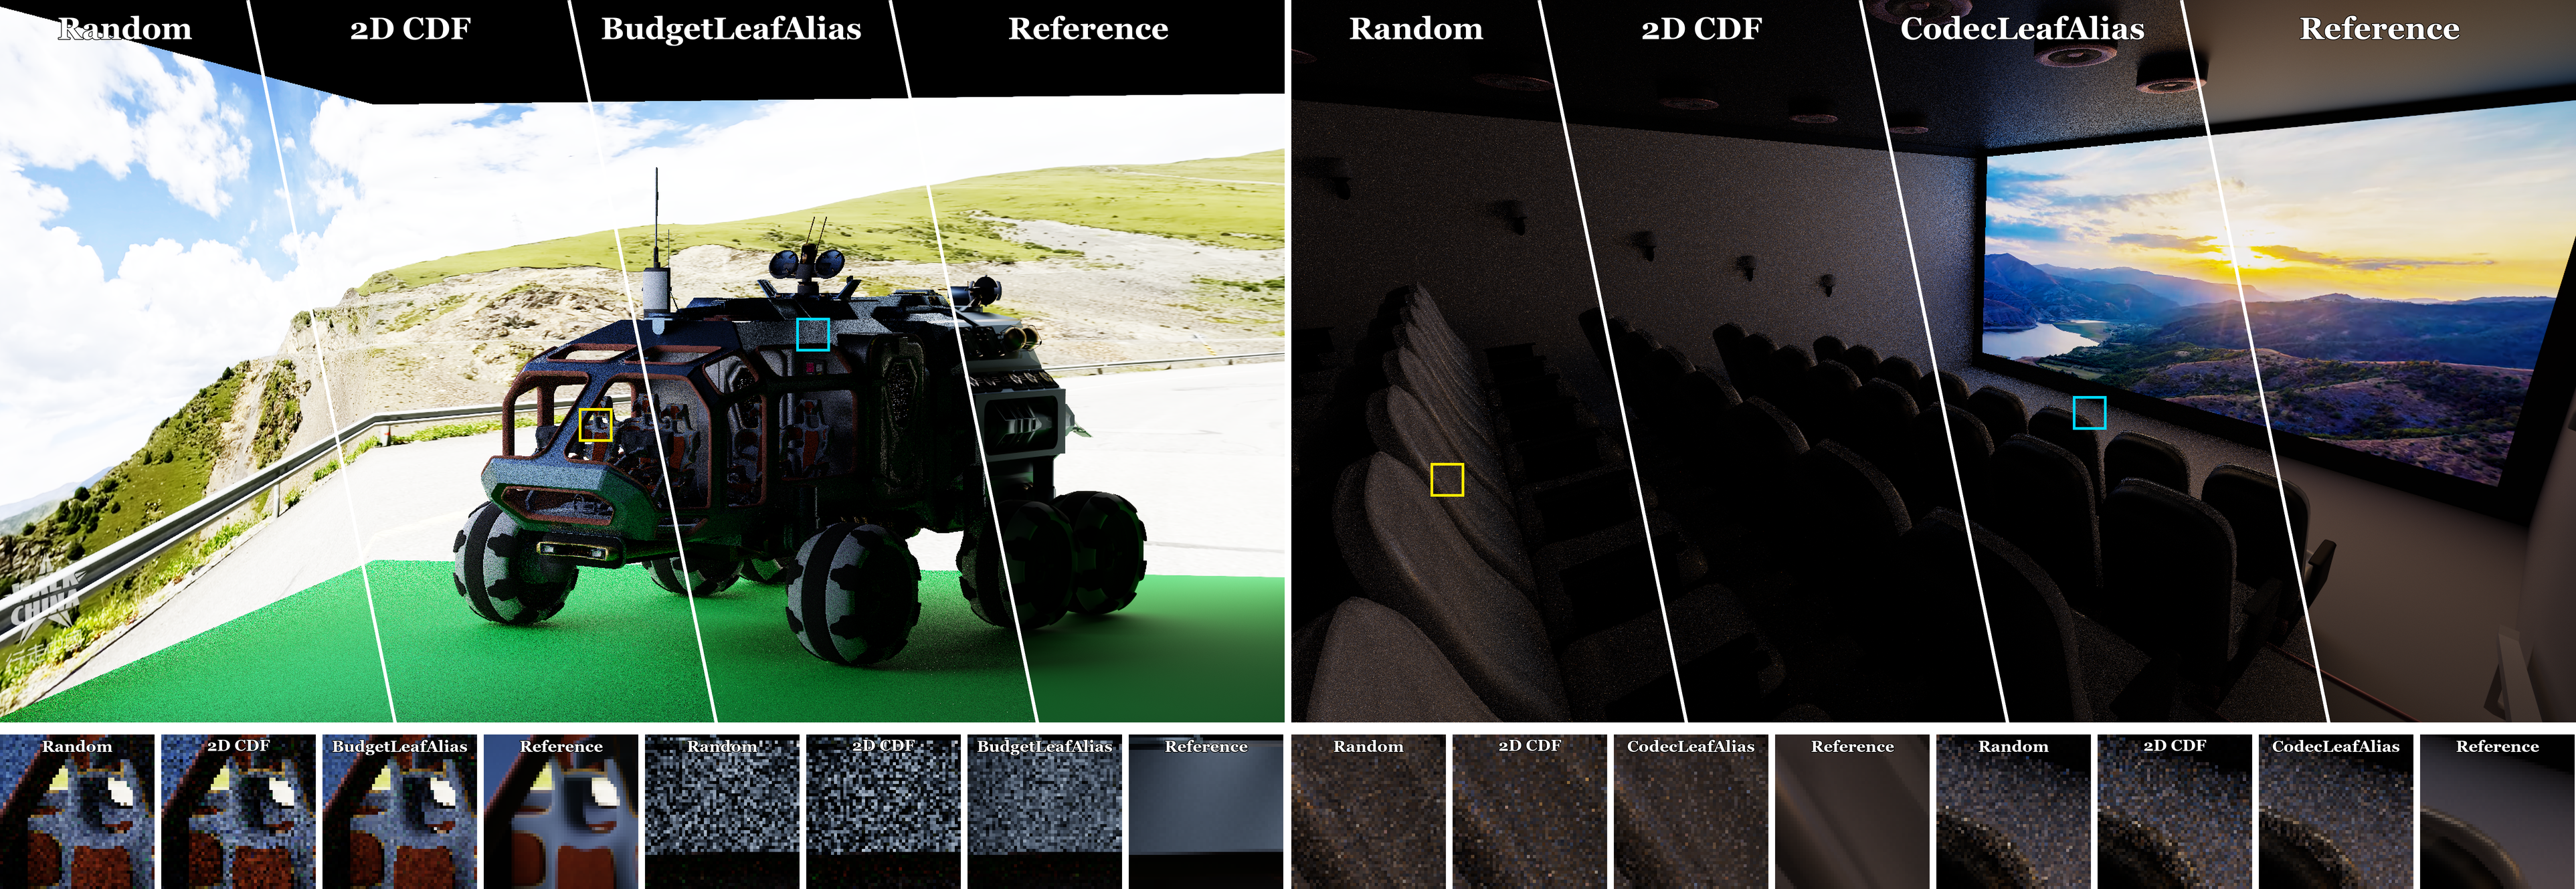
\includegraphics[width=1\textwidth]{teaser.png}
  \caption{Two scenes lit by a single dynamic, video-driven emissive texture, rendered with our LeafAlias importance sampler. (Left) The Rover scene — a virtual-production LED wall displaying a looping road/mountain video panorama that lights the vehicle directly, sampled here with BudgetLeafAlias. (Right) The Cinema scene — a theater lit only by the animated sunset footage playing on its own screen, sampled with CodecLeafAlias. Each panel compares, left to right: Random sampling, 2D CDF inversion, our technique, and a converged reference, all at their calibrated real-time budgets ($\approx$33 ms).}
  \label{fig:teaser}
\end{teaserfigure}

%%
%% This command processes the author and affiliation and title
%% information and builds the first part of the formatted document.
\maketitle

\section{Introduction}

Importance sampling of emissive textures is essential for efficient image-based lighting, and increasingly critical in production and VFX workflows where video is used directly as a dynamic light source. A single emissive texture lets a renderer reproduce the directional detail of a real environment far beyond what analytic lights can approximate. Traditionally, this texture has been static: captured once and reused for an entire sequence. However, there are recent use cases such as LED-wall virtual production, AR/VR object insertion, and video-based environment maps that require illumination that changes every frame.

\rev{The texture light samplers found in current renderers are designed for static images.} They rely on offline construction of large sampling structures that are stored and reused. The most common example of this strategy is how rendering and ray tracing toolboxes deal with HDR environment maps. The standard approach is to build a two-dimensional piecewise-constant distribution from the texture's luminance: a marginal CDF over rows and a per-row conditional CDF. The sampler is then inverted via binary search at sample time, which is expensive and produces incoherent memory access. A more recent and well-adopted approach is to generate a mipmap-style hierarchical importance map \cite{clarberg2005wavelet}. At sample time, a hierarchical descent through a mip pyramid
of the texture is performed, recursively choosing one of four children at each level in proportion to their summed weight. This technique is also expensive and requires several iterations per sample, although it is more GPU-friendly because the number of iterations is always the same for each sample, unlike with the binary search. Moreover, the mipmap can be constructed quickly using the existing dedicated hardware on modern GPUs. Both techniques require at least $O(N)$ memory for the sampler, with $N$ being the number of pixels.

Another less used but known technique for sampling emissive textures is the Alias method \cite{burke2004bidirectional}. This technique draws from an arbitrary discrete distribution in $O(1)$ time after an $O(N)$ one-time build, at the cost of losing the CDF's implicit spatial coherence: two adjacent table buckets can alias to two arbitrary, unrelated locations in the original distribution. This fact is known to disrupt stratification or discrepancy reduction of the input point set. It also requires $O(N)$ memory to store the correlation between every pixel. The process for building the Alias table, despite being $O(N)$, is difficult to optimize for real-time construction \cite{lehmann2021weighted}.

We present a new sampling method that is fast to build, produces a sampler that is tiny, \rev{is $O(1)$ to sample, and does not create the structured sample patterns that the per-pixel Alias method can produce.} The core idea is to reuse the variance-driven image partition that is already present in modern video codecs, which already compute hierarchical spatial partitions that adapt to local signal variance \cite{uhrina2024performance}. These structures implicitly encode the spatial distribution
of luminance and high-frequency content (see Fig. \ref{fig:quadtree}). We also propose a variant that builds the partition tree on a budgeted number of leaves, using a  Greedy/best-first tree-structured resource allocation strategy \cite{MINASNY2007383,Zhou2024}. \rev{Both techniques render video light textures in real time (33 milliseconds per frame) with consistent gains, because each of their samples is cheaper and more of them fit in the frame.}

\newbegin
Our samplers are per frame by design: each frame's structure is built from that frame alone, with no knowledge of past or future frames. Their purpose is not to sample a frame more accurately than an exact per-texel distribution, which is not possible, but to approach its accuracy with a structure that is orders of magnitude smaller and cheaper to build and to sample. Our contributions are:
\begin{itemize}
\item LeafAlias, an alias table over the leaves of a variance-driven partition of the texture, with $O(1)$ sampling and an $O(1)$ density lookup for multiple importance sampling, in a structure of tens of kilobytes.
\item Two sources for the partition: the coding tree of a video codec, with a study of how leaf radiance is obtained from coded data and how quantization, bitrate, codec family and encoder configuration affect it; and a greedy quadtree with a fixed leaf budget.
\item An evaluation that separates the quality of the sampling density (equal samples) from its cost (equal quality), over full videos and against per-texel baselines, together with studies of the leaf budget and its relation to the GPU cache, of static against per-frame partitions, and of temporal stability.
\end{itemize}
\newend

\begin{figure}[htbp!]
  \centering
  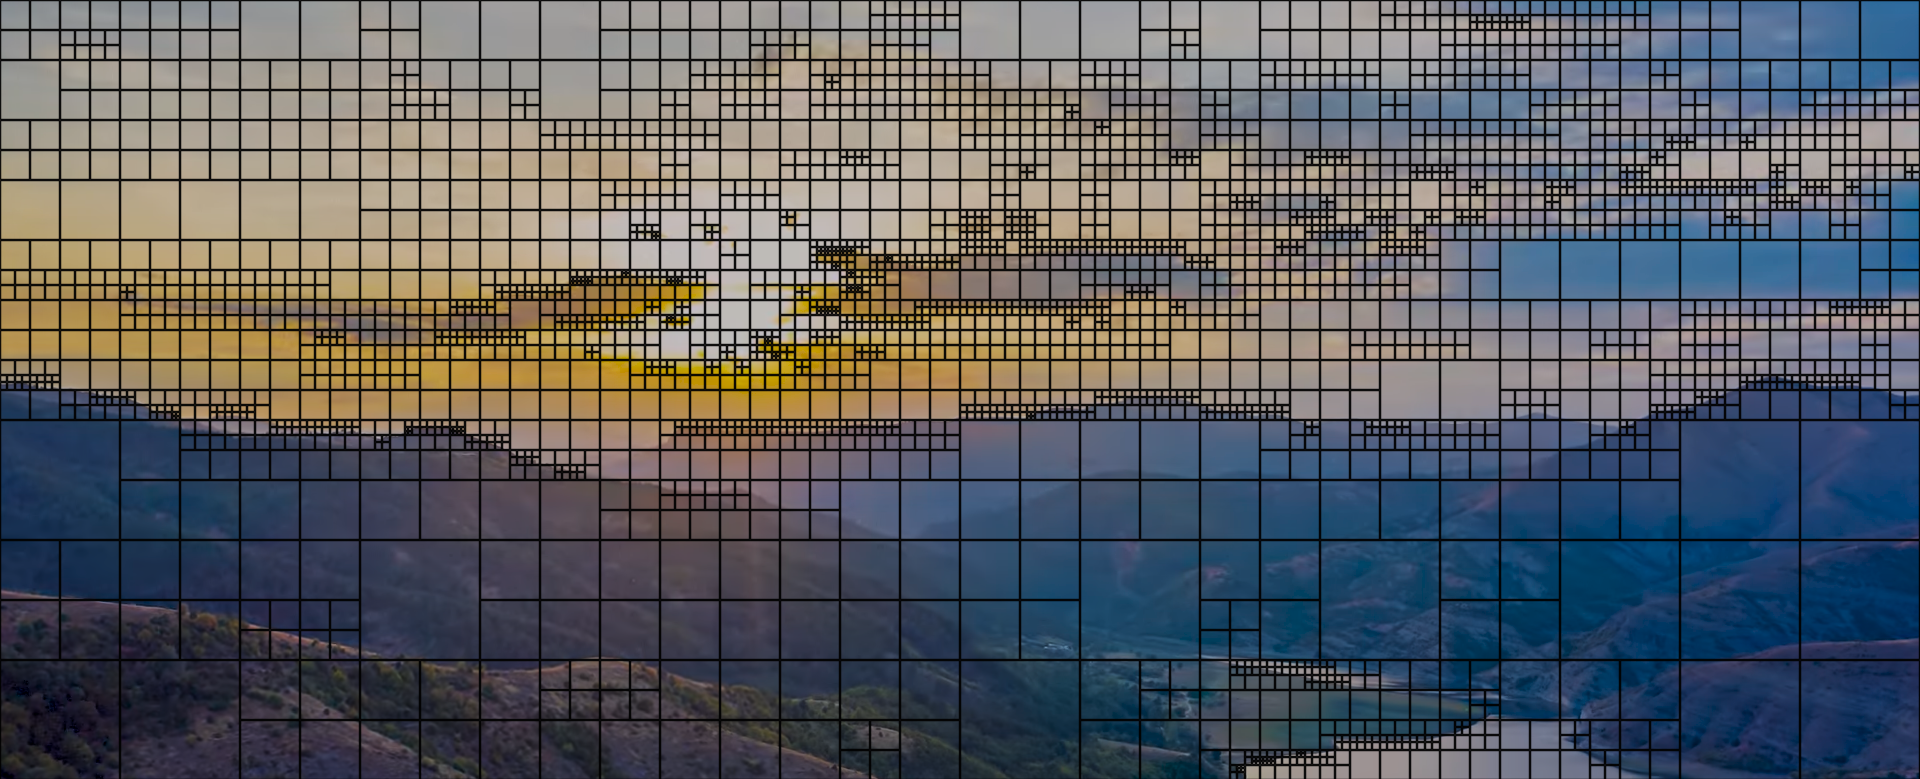
\includegraphics[width=\linewidth]{quadtree.png}
  \caption{An example of a variance-driven quadtree built by the VP9 video codec. High-variance zones are refined into a dense mesh of
  small cells.}
  \label{fig:quadtree}
\end{figure}

\new{
\section{Motivation}

\paragraph{Real-time path tracing in games.}
Light sampling with spatiotemporal resampling draws its initial candidates from
tabulated distributions over emissive geometry and environment maps
\cite{bitterli2020spatiotemporal}, and the cost of rebuilding those tables is a known
obstacle to dynamic content. Wyman and Panteleev~\cite{wyman2021rearchitecting} report the cost of
alias-table builds for large environment maps as one of the main challenges in presampling lights, and instead propose
a GPU-accelerated MIP structure to process textures coming from light probes streamed live from a 360 camera. The quality
of these initial candidates still bounds the result and limits resampling \cite{zeng2025restirpg}, and the integration
of ReSTIR in a shipped path-traced game lists initial candidate sampling quality among
its main sensitivities, with emissive surfaces and the skylight left to BSDF sampling
\cite{kozlowski2023cyberpunk}. Production engines report the same pressure from
content. Lumen lights scenes with emissive surfaces but notes how small
and bright areas cause noise artifacts, and names
explicit sampling of emissive meshes as future work \cite{wright2022lumen}; its
successor for direct lighting observes that artists now use rectangular and textured
lights more frequently \cite{narkowicz2025megalights}. Current guidance for path-traced
games recommends environment maps that are baked every frame so that dynamic skies and
clouds can be importance sampled, and a dedicated sampling structure for signs,
animated effects and procedural emissive materials \cite{nvidia2026ptwhitepaper}.
Recent work still describes the evaluation of many lights per pixel as a major
bottleneck of real-time rendering \cite{chen2026lightopt}.

\paragraph{Virtual production.}
On an LED stage the wall is at once the in-camera background and the light source of
the scene: the stage is driven as an image-based lighting instrument
\cite{debevec2022dilation,legendre2022jointly}, and the video that
drives the wall also drives the lighting fixtures around it \cite{bengtsson2022ibl}.
While the camera rolls, the panels light the real actors physically. The rendering
problem appears whenever the subject under that light is synthetic, and this happens
at three points of a production. Before the shoot, the lighting of a volume is designed
in simulation: productions go through a prelight in the virtual art department, where
the engine reproduces the environment as it will appear on the screens
\cite{kadner2023stages,zwerman2023ves}, techvis rebuilds the on-set hardware as a 3D
scene \cite{failes2024hotd}, and digitized performers are previsualized inside the
virtual stage \cite{nash2025integration}. Such previsualization of panel-generated lighting effects is older than the LED volume \cite{bunish2017rogueone,seymour2013gravity,hamon2014gravity}. During the shoot, when a shot cannot be finished
in camera, the camera frustum is keyed and provisional imagery is composited live
while the rest of the wall keeps lighting the subjects \cite{kadner2021fieldguide}.
After the shoot, the creatures and environments of such shots are added in post
\cite{failes2022hotd} and have to match the lighting that the wall gave the actors.
Research has started to treat the wall accordingly, as a near-field, high-resolution
textured emitter whose image is known at every frame \cite{azzarelli2026relightable},
and to use LED stages to reproduce per-frame HDR environment maps at video rate
\cite{zhang2026pixelcube}. In all of these cases a renderer lights a synthetic subject
with a video, and its sampling structure has to follow that video frame by frame.

\paragraph{Mixed reality and telepresence.}
In augmented and mixed reality the illumination is captured
or estimated while the application runs. HDR environment maps are inferred from the
camera feed at interactive rates on mobile devices
\cite{legendre2019deeplight,somanath2021hdr,zhao2021xihe}, estimated consistently over
video \cite{li2023spatiotemporally,shen2025stglight,bolduc2026limo}, or taken directly
from a live $360^\circ$ stream with changing real-world lights
\cite{rhee2017mr360,rhee2018mr360live,walton2018dynamic}. For such high-frequency
illumination, importance sampling of the environment map is essential for efficient
rendering \cite{kronander2015photorealistic,alhakamy2020realtime}. Systems that do
path trace under a live panorama on a head-mounted display report that the result must
be denoised \cite{cheng2023environment,wu2024panoramic}, and that in a headset Monte
Carlo noise is more than a quality problem, since its temporal flicker aggravates
cybersickness \cite{taibo2024immersive}. Most real-time systems therefore avoid
sampling: they prefilter the map or reduce it to a few dominant lights\cite{saito2024relightable}. A sampling structure that can be rebuilt at
the rate of the display, and that is small enough to keep one per light, is a
precondition for moving these applications from prefiltered shading to path tracing
with correct shadows and interreflections.
}
\section{Previous works}\label{sec:prev}
Importance sampling of emissive textures is a well-studied problem in the graphics literature in the context of image-based lighting. Most of the works focus on preprocessing the images to allow for exact or near-exact sampling without introducing bias \cite{lawrence2005adaptive}. Several methods choose to simplify the textured light into a set of point or area lights ~\cite{agarwal2003structured}, allowing for real-time sampling and faster convergence but at the cost of more error in the solution. \cite{cline2009tabular} compare several tabular inversion methods, noting the computational order of building each sampler structure and sampling each point. They analyze the 2D CDF inversion via binary search and the per-pixel Alias method, where they flag the disruption of the stratification of the input point set. \rev{With a low-discrepancy input, the raster-flattened table of the per-pixel Alias method can produce a measurable periodic banding pattern (Figure~\ref{fig:spectrum}) that becomes clear in the power spectrum of the sample set. Appendix~\ref{app:qmc} analyzes these effects and their consequence in a rendering for our proposed methods and compares it with per-pixel Alais.}

\begin{figure}[htbp!]
  \centering
  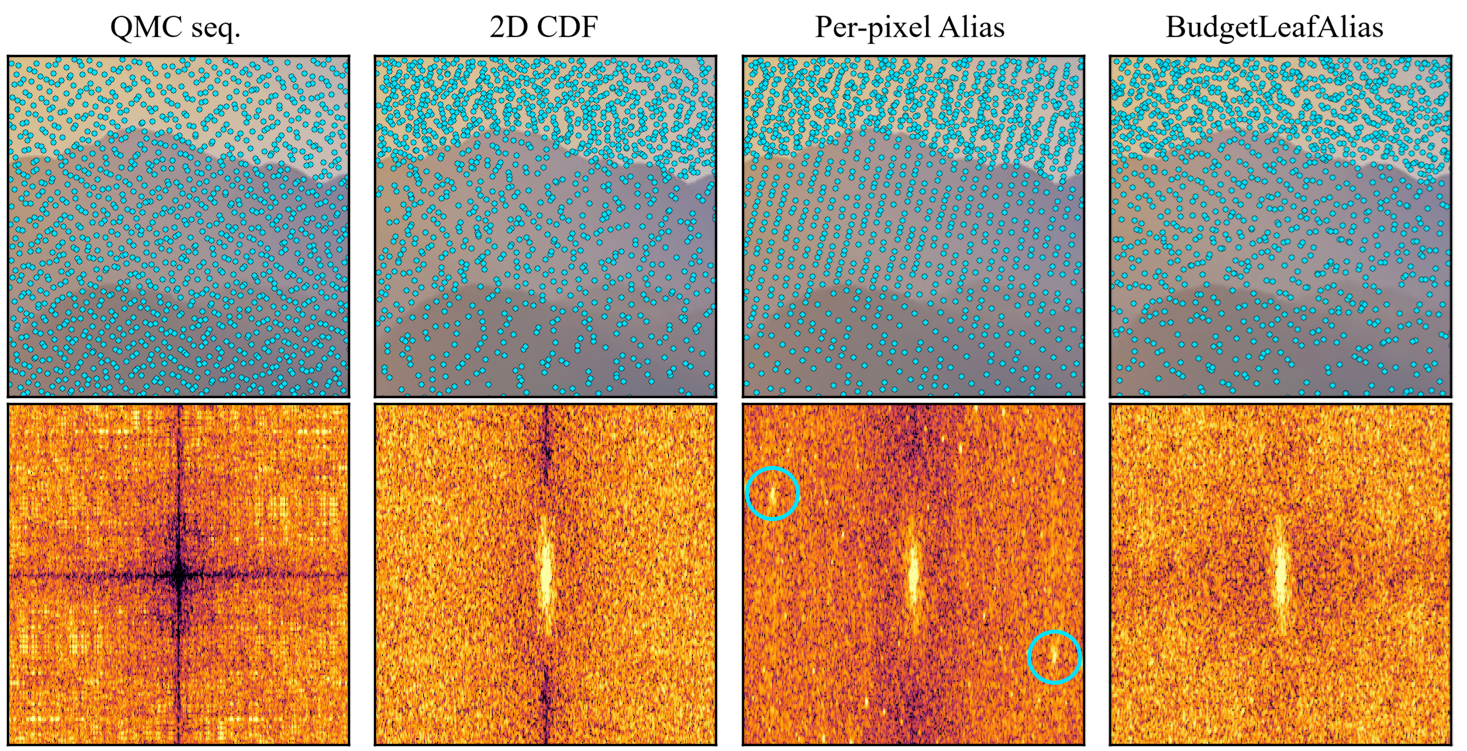
\includegraphics[width=\linewidth]{fig_spectrum_paper_color.png}
  \caption{2D power spectrum of samples from 2D CDF inversion, plain per-pixel alias, and
  our LeafAlias, from the same Halton input. Per-pixel alias shows a sharp,
  isolated off-axis peak (flatness 0.270, peak/median 16{,}113), a periodic banding
  artifact from its flat array index resonating with the input sequence's base-2 digit
  structure.}
  \label{fig:spectrum}
\end{figure}

Despite being $O(1)$ to sample, the Alias method is memory-intensive and expensive to construct via Vose's technique.
Nevertheless, it is widely used in mesh light sampling for geometry with thousands of emissive triangles. \cite{moreau2019dynamic} maintain a light-sampling BVH incrementally across frames for thousands of moving lights.
ReSTIR~\cite{bitterli2020spatiotemporal} resamples across spatial and
temporal neighbors to pick among many dynamic lights at a fraction of the cost of resampling
from scratch. Conty Estevez and Kulla~\cite{contykulla2018adaptive} adaptively split a light
tree per shading point rather than committing to one fixed cut. At that scale of thousands of triangles, a plain alias table over per-triangle flux is common practice
and cheap to rebuild every frame.

Regarding the optimization of the sampling structures,
\cite{ergun2012realtime} split an environment map into a kd-tree via the greedy partition strategy, to a predefined block count, then fit the sorted leaf probabilities with an approximate analytic curve for direct inversion. They report gains in memory compression, higher speed and accuracy than CDF inversion at matched performance for static environment maps. One disadvantage of using kd-trees is that evaluating the pdf of the map direction when sampled from the BRDF in multiple importance sampling (MIS) requires traversing the tree.
 Lambers~\cite{lambers2022parameterization} proposes a fixed-grid sampler and notes that replacing the grid with a variance-driven quadtree might improve their results. \cite{rodriguez2023nenv} train a neural normalizing flow that allows both sampling and evaluating the pdf, showing considerable performance gains at the cost of pre-training the structure for the static map. Wu~\cite{wu2025efficient} also preprocesses the map by dividing the emissive and non-emissive parts into separate structures. \new{Sz\'ecsi et al.~\cite{szecsi2010adaptive} adapt the placement of the samples of an environment map on the GPU, taking the reflectance at the shading point into account as well as the illumination. Sampling densities that depend on the shading point, like \cite{szecsi2010adaptive}, MIS-compensated distributions~\cite{karlik2019mis} or variance-aware guiding~\cite{rath2020variance}, are complementary to our work, which builds a scene-independent density from the texture alone.}

\rev{The previously described techniques focus mainly on preprocessing static images to improve sampling efficiency. Sampling of dynamic environment maps has also been studied.} \new{Wan et al.~\cite{wan2005q2tree} subdivide the sphere into a Q2-tree of quadrilaterals according to illumination importance and generate a temporally coherent set of directional samples for every frame of an environment sequence. Wan et al.~\cite{wan2011spatiotemporal} treat the whole sequence as a spatiotemporal volume and stratify the samples in space and time, and Yang et al.~\cite{yang2014high} extend this line to high-dynamic-range sequences. These methods exploit temporal coherence, and the spatiotemporal ones analyze the sequence as a whole before rendering, which suits recorded content. Our method works on the current frame only, so it applies to live video, and it produces a density that can be sampled and evaluated for MIS inside a path tracer, rather than a fixed set of light directions.} \rev{Other works address video-driven lighting:} \cite{havran2005interactive} and Iorns and Rhee~\cite{iorns2015realtime} both light scenes from captured video environment maps, but neither targets real-time per-frame
resampling of the video itself as the importance distribution. \cite{lu2013realtime} rebuild a tabulated per-cube-face CDF in real-time, noting it as an expensive part of the process. \cite{kronander2014real} rely on temporal sample reuse to improve convergence of video-based lighting.

Attempts to make the per-frame rebuild itself cheaper on a GPU point in the same direction: Morrical and Zellmann~\cite{morrical2021inverse} accelerate 2D CDF
inversion with ray tracing hardware at a high construction cost and non-trivial implementation
complexity. \cite{lehmann2021weighted} study GPU-specific weighted sampling and alias-table construction directly. \new{Binder and Keller~\cite{binder2019radix} build radix tree forests in parallel on the GPU to sample discrete distributions with a monotone mapping. These approaches make a per-texel structure faster to build; ours reduces the size of the structure instead, which lowers the cost of building it, storing it and sampling it at once.}

Modern production renderers mostly rely on dense CDF or mipmapped samplers. {Falcor}~\cite{falcorsoftware} uses a hierarchical mip-pyramid importance map over the environment texture's luminance and, separately,
the triangle-scale alias table for mesh lights. {Mitsuba 3}~\cite{nimierdavid2019mitsuba2} builds a {Hierarchical2D} warp over
the environment map, which is the same mip-pyramid family as Falcor's. {pbrt-v4}~\cite{pharr2023pbrt}
uses a dense CDF distribution, inverted via binary search. {Blender Cycles}~\cite{cyclessoftware} builds the same
kind of dense marginal/conditional CDF over a downsampled background map.

\section{Method}\label{sec:method}

The LeafAlias technique applies to any light source described by a 2D radiance texture $L(u,v)$ over
a parameter domain $(u,v)\in[0,1)^2$, e.g. an environment map, or the emission texture of an
area light. As with any textured light, variance is minimized when the sampling density
matches radiance, $p(u,v)\propto L(u,v)$. We approximate this with a piecewise-constant density
over a partition of the domain into disjoint leaf rectangles $\{R_i\}_{i=1}^N$, for now
assumed given; Sections \ref{sec:codec} and \ref{sec:budget} describe the two ways we
actually construct it. Each leaf carries a single weight proportional to its flux: its area in the parameter domain
times its average radiance:
\begin{equation}
w_i = A_i \bar{L}_i, \qquad \bar{L}_i = \frac{1}{A_i}\int_{R_i} L(u,v)\,dA. \label{eq:weight}
\end{equation}
Normalizing over all leaves gives a piecewise-constant density over the parameter domain
and a per-leaf selection probability:
\begin{equation}
p(u,v) = \frac{\bar{L}_i}{W} \ \text{for } (u,v) \in R_i, \qquad
p_i = \frac{w_i}{W}, \qquad W = \sum_{j=1}^N w_j. \label{eq:pdf}
\end{equation}
Converting $p(u,v)$ to whatever measure a particular light type actually samples with
respect to (solid angle for a distant environment map or projected solid angle for a local
area light) is a standard change-of-variables applied at evaluation time, and is
independent of the sampling structure described below.

Given the partition, we flatten it into an array of $N$ leaves, each storing its rectangle
and weight $w_i$ from Equation~\ref{eq:weight}. We build a Walker/Vose alias
table~\cite{vose1991linear} over this array once, in $O(N)$: leaves below the mean weight
are paired with leaves above it, the excess of the latter absorbs the deficit of the
former, and the process repeats until every leaf holds a threshold and, where needed, the
index of the leaf it aliases to (Algorithm~\ref{alg:build}). Unlike a dense CDF, the
resulting table needs no search at sample time since selecting a leaf is an $O(1)$ array
lookup.

\begin{algorithm}[h]
\caption{Build the alias table over $N$ leaves}
\label{alg:build}
\begin{algorithmic}[1]
\STATE $W \leftarrow \text{mean}(w_1,\dots,w_N)$
\STATE partition leaf indices into \textit{small} ($w_i < W$) and \textit{large} ($w_i \geq W$)
\WHILE{\textit{small} and \textit{large} both non-empty}
  \STATE $s \leftarrow$ pop(\textit{small}); \quad $l \leftarrow$ pop(\textit{large})
  \STATE $\mathit{threshold}[s] \leftarrow w_s / W$; \quad $\mathit{alias}[s] \leftarrow l$
  \STATE $w_l \leftarrow w_l - (W - w_s)$ \COMMENT{transfer $l$'s excess weight to $s$}
  \STATE push $l$ back onto \textit{small} or \textit{large} by its updated $w_l$
\ENDWHILE
\FOR{remaining $i$ in \textit{small} $\cup$ \textit{large}}
  \STATE $\mathit{threshold}[i] \leftarrow 1$
\ENDFOR
\end{algorithmic}
\end{algorithm}

\subsection{Sampling}
\label{sec:sampling}
To draw a light sample, we use three uniform numbers $\xi_1,\xi_2,\xi_3$
(Algorithm~\ref{alg:sample}). $\xi_1$ selects a bucket in $O(1)$;
$\xi_2$ decides whether we keep that leaf or its
alias partner.
$\xi_3$ and $f$ place the sample uniformly
inside the chosen leaf's rectangle. The sample's pdf is read directly from its
leaf's stored average luminance via Equation~\ref{eq:pdf}. Radiance is read from the texture at the sampled $(u,v)$.

\begin{algorithm}[h]
\caption{Draw one light sample}
\label{alg:sample}
\begin{algorithmic}[1]
\STATE $i \leftarrow \lfloor \xi_1 N \rfloor$; \quad $f \leftarrow \xi_1 N - i$
\IF{$\xi_2 < \mathit{threshold}[i]$}
  \STATE $\mathit{leaf} \leftarrow i$
\ELSE
  \STATE $\mathit{leaf} \leftarrow \mathit{alias}[i]$
\ENDIF
\STATE $(u,v) \leftarrow \text{lerp}(R_{\mathit{leaf}}.\mathit{min}, R_{\mathit{leaf}}.\mathit{max},\, (f,\xi_3))$
\STATE \textbf{return} $(u,v)$, $\;p(y){=}\bar{L}_{\mathit{leaf}}/W$ (Eq.~\ref{eq:pdf}), $\;L(u,v)$
\end{algorithmic}
\end{algorithm}

Combining light sampling with BRDF sampling via MIS requires the
reverse query: given a direction chosen by BRDF sampling that happens to hit the light at
some $(u,v)$, the probability $p(y)$ is needed. Rather than searching the partition, we
maintain a small auxiliary lookup matrix that maps a coarsened $(u,v)$ coordinate directly to
its leaf index, at a fixed fraction of the texture's resolution matching the partition's
smallest possible leaf (e.g.\ one entry per $8{\times}8$ block).
Every coordinate covered by a given leaf is written to the same entry at
construction time, so the lookup is an $O(1)$ array read that reproduces the exact same
$\bar{L}_i/W$ used at sampling time regardless of that leaf's actual size, keeping the
resulting MIS weight unbiased. We also tried replacing this exact lookup with a single
scene-wide average density: across our test scenes this produced no perceptible difference
in the rendered images, but it does introduce bias, since the substituted value no longer
matches the technique's actual density at that point.

\subsection{CodecLeafAlias}
\label{sec:codec}
Building the partition can be costly, especially for dynamic content that changes every few milliseconds.
CodecLeafAlias avoids it entirely when the texture
arrives as a compressed video frame. Modern codecs (HEVC, AV1, VP9) already split each frame
into a coding-tree hierarchy driven by local signal variance, which is structurally the same
partition our method needs.
We take each coding-tree leaf's block directly as one of our leaf rectangles $R_i$, and
estimate $\bar{L}_i$ from the block's own zero-frequency (DC) transform coefficient rather
than summing pixels: the DCT/DST's DC term is, up to a fixed normalization constant, exactly
the block's mean sample value, and is already computed and present in decoder metadata.
\newbegin
The DC coefficient gives the mean of a block of the \emph{coded} signal, which for HDR video is a nonlinear, quantized $Y'C_bC_r$ signal (10-bit PQ, BT.2100, in our experiments), so three steps separate it from $\bar{L}_i$. (1)~The reconstructed block mean of each plane is its dequantized DC divided by the transform gain. For a block coded with prediction, the DC belongs to the residual, and the mean of the prediction (extracted from the decoding process) must be added. (2)~The three means are converted to $R'G'B'$ with the BT.2020 matrix, linearized with the PQ transfer function, and transformed to luminance with the BT.2020 weights. (3)~The result is multiplied by the leaf area to give $w_i$ (Eq.~\ref{eq:weight}). This process and quantization perturb the DC, and therefore the density of Eq.~\ref{eq:pdf}, but not the expected value of the estimator: every sample is divided by the density actually used, so the estimate stays unbiased for any density that is positive wherever the emitter is. We keep a small density floor ($10^{-4}$ of the mean weight) so that no lit leaf is quantized to zero. A wrong weight can therefore only add variance; Section~\ref{sec:codecstudy} measures the effect of quantization in the results.
\newend

In our experiments, we encode the dynamic emissive textures as HDR video using libvpx's VP9 Profile 2 and extract the superblocks for each frame via decoder statistics. We configure the encoder to always use variance-based superblock partitioning. Encoder settings that instead search or reuse partitions (full rate-distortion search, predicted neural partitions, etc.) \new{can} still supply a usable partition by combining each block's motion vector with its keyframe's already-computed superblocks. \new{Section~\ref{sec:codecstudy} evaluates this strategy, other codec families and the effect of bitrate.} 

Using codec partitions results in varying number of leaves, ranging from 4000 to 20000 depending on the content. We call this method CodecLeafAlias. Since the sampling algorithms are memory-bound operations, we go further by defining a new partition mechanism that allows us to choose a budgeted number of leaves to reduce memory needs and improve coherence. We call this other method BudgetLeafAlias.

\subsection{BudgetLeafAlias}
\label{sec:budget}
BudgetLeafAlias constructs the quadtree directly from the texture under a hard
leaf-count budget $B$ (in our implementation, matched to what fits alongside the alias
table in a modern GPU's L1 data cache; Section~\ref{sec:impl}). Rather than recursing to a
fixed depth or a fixed per-node threshold, we spend the budget greedily
(Algorithm~\ref{alg:budget}): a priority queue always refines whichever pending block
currently contributes the most summed-squared error to the piecewise-constant
approximation, $\mathrm{Var}(R)\cdot A(R)$, until the budget is exhausted or no block has
positive variance left to resolve. This is the standard greedy construction for a
budget-constrained piecewise-constant approximation: unlike a fixed-depth or
fixed-threshold rule, it spends every one of its $B$ leaves wherever the source image
actually has the most error left to remove.

\begin{algorithm}[h]
\caption{Build a budgeted quadtree of $\leq B$ leaves}
\label{alg:budget}
\begin{algorithmic}[1]
\STATE $\mathit{queue} \leftarrow \{\mathit{root}\}$; \quad $\mathit{leaves} \leftarrow \emptyset$
\WHILE{$\mathit{queue} \neq \emptyset$ and $|\mathit{leaves}| + |\mathit{queue}| + 3 \leq B$}
  \STATE $R \leftarrow$ pop block with max $\mathrm{Var}(R)\cdot A(R)$ from $\mathit{queue}$
  \FOR{each of the 4 children $C$ of $R$}
    \IF{$C$ is $8{\times}8$ texels or smaller, or $\mathrm{Var}(C) = 0$}
      \STATE $\mathit{leaves} \leftarrow \mathit{leaves} \cup \{C\}$
    \ELSE
      \STATE $\mathit{queue} \leftarrow \mathit{queue} \cup \{C\}$
    \ENDIF
  \ENDFOR
\ENDWHILE
\STATE $\mathit{leaves} \leftarrow \mathit{leaves} \cup \mathit{queue}$
\end{algorithmic}
\end{algorithm}

\subsection{Implementation}
\label{sec:impl}
\rev{We implement both variants in NVIDIA's Falcor rendering engine and test using a full path tracer with MIS: one BSDF sample per bounce, and a configurable number of light samples per shading point, each weighted against BSDF sampling.}
We construct the LeafAlias tables and partitions in the CPU, and pass the results to the GPU in each frame.
All the precomputation is done in under 1 millisecond per frame. We implement the sampling method in the Slang Shading Language.
In order to reduce GPU memory usage and improve coherency, we spent some effort in making the sampling structures as small as possible.
Each leaf is packed into a 16-byte record, its rectangle as two packed 16-bit corner coordinates, the alias threshold and redirect index
as a half-float and a 16-bit index, and $\bar{L}_i$ as a half-float. For BudgetLeafAlias, we size $B$ so the combined leaf and node buffers fit within roughly half of the GPU's per-core L1 cache, keeping the whole sampling structure resident there during
traversal instead of round-tripping to global memory on every sample. \rev{With $B=4000$ the structure takes 75\,KB. This compactness helps improve performance when compared to other memory-bound samplers like dense CDF or per-pixel Alias table; Section~\ref{sec:leafbudget} measures the effect of $B$ on quality and on cost.}

\section{Results} \label{sec:results}

All experiments run on an Intel Core i7-14700F CPU and an NVIDIA GeForce RTX 4080 SUPER GPU (128\,kB of L1 cache/shared memory per streaming
multiprocessor). We evaluate seven real-time techniques across our five scenes
(LED-wall Rover, projector-lit Cinema, Fireplace Room, Phone, and the multi-material
Convergence scene): uniform random sampling; dense 2D CDF inversion; the same CDF built at $1/8$ resolution; a hierarchical
mipmap-warp sampler; a per-pixel Alias table; and our
own {BudgetLeafAlias} and {CodecLeafAlias}. We added 2D CDF/8 to analyze the quality and performance
tradeoffs of a coarser resolution; we also tested several further resolution-trimming factors beyond $1/8$ (down to $1/16$ and $1/32$)
and observed the same trend: smaller resolutions are cheaper to sample but significant error is introduced. We report only the $1/8$ variant in what follows, as the representative trimmed-resolution case.

All techniques are implemented in Falcor, with particular
attention paid to making the GPU-side sampling code efficient for each technique. The CPU-side cost
of building each sampling structure for every frame varies considerably: 2D CDF's
dense per-pixel CDF costs approximately $10$\,ms per Full HD frame, while per-pixel Alias table costs approximately $30$\,ms; our own technique's
leaf-budgeted construction is consistently under $1$\,ms per frame across every scene tested. The sampling parameters for each technique (samples per pixel and light samples per vertex) are tuned per scene to a real-time budget of $33$\,ms (30\,fps) using the same calibration procedure. 
 \new{Since we are interested in analyzing the sampler efficiency, not the structures build time, we leave the build time out of the calibration, so the presented real-time results only consider sampling performance. }
2D CDF and mipmapped methods allow approximately a third of the samples obtained with the random approach. BudgetLeafAlias allows the same number of samples as random, while CodecLeafAlias and per-pixel alias allow approximately 25\% fewer. \new{Table~\ref{tab:configs} lists the configurations. BudgetLeafAlias uses $B=4000$ leaves unless stated otherwise.}

\begin{table}[htbp!]
\centering\small\newmat
\setlength{\tabcolsep}{3pt}
\caption{\newmat Calibrated real-time configuration of each technique per scene: samples per pixel $\times$ light samples per shading point, each within the 33\,ms frame. }
\label{tab:configs}
\resizebox{\columnwidth}{!}{%
\begin{tabular}{l ccccccc}
\toprule
Scene & \shortstack{Random} & \shortstack{2D CDF} & \shortstack{2D CDF/8} & \shortstack{Mipmap} & \shortstack{Per-pixel\\Alias} & \shortstack{Budget\\LeafAlias} & \shortstack{Codec\\LeafAlias} \\
\midrule
Rover & 4$\times$19 & 4$\times$5 & 4$\times$12 & 4$\times$9 & 4$\times$13 & {4$\times$19} & 4$\times$15 \\
Cinema & 4$\times$8 & 4$\times$2 & 4$\times$4 & 4$\times$3 & 4$\times$5 & {4$\times$8} & {4$\times$8} \\
Fireplace Room & 4$\times$5 & 4$\times$2 & 4$\times$2 & 4$\times$2 & 4$\times$3 & {4$\times$5} & {4$\times$4} \\
Phone & 16$\times$10 & 16$\times$3 & 16$\times$5 & 16$\times$3 & 16$\times$7 & {16$\times$10} & {16$\times$8} \\
Convergence & 4$\times$3 & 4$\times$1 & 4$\times$2 & 4$\times$1 & 4$\times$2 & {4$\times$3} & {4$\times$3} \\
\bottomrule
\end{tabular}}
\end{table}

Each scene is lit by a different HDR video played back as the
scene's only light source: Rover uses a Full HD road/mountain driving sequence
(600 frames) displayed on a virtual-production LED wall; Cinema uses a Full HD
sunset-landscape sequence (250 frames) with a small, very bright sun; Fireplace Room uses a 4K real fire video (800 frames); Phone uses
a Full HD abstract color sequence (1200 frames); and
Convergence uses a 4K dark cave with multiple bright lights video (800 frames) as a single environment map. Altogether, across these five sequences, our techniques are evaluated against thousands of distinct HDR emissive
textures, not just the one representative frame shown in each figure. The resulting videos are found in the supplementary material.

\new{The evaluation is organized around three questions. Section~\ref{sec:video} reports the quality of every technique over the full videos at its real-time configuration. Section~\ref{sec:equalsamples} removes the cost of sampling from the comparison (equal samples), to measure what the leaf approximation loses. Section~\ref{sec:equalquality} measures what its lower cost gains (time to equal quality). The remaining sections analyze the cost itself, the leaf budget, the need for a per-frame partition, and the codec variant.}

\subsection{\texorpdfstring{\revt{Full-video quality}}{Full-video quality}}
\label{sec:video}

\newbegin
For each scene we render regularly spaced frames spanning the whole video. Each frame is compared with a converged reference of the same frame, without denoising. RMSE is computed per frame on the tone-mapped output and averaged over frames, as well as PSNR; VMAF is computed on the frame sequence of each technique against the reference sequence. We report each mean with its 95\% confidence interval over frames.

Table~\ref{tab:main} reports RMSE, PSNR and VMAF for all seven techniques on all five scenes. On every scene, one of our two techniques has the best mean on all three metrics: BudgetLeafAlias on Rover, Cinema and Phone, CodecLeafAlias on Fireplace Room and Convergence. Relative to the 2D CDF, the best of our two techniques lowers the video RMSE by up to 23\%. The gains hold over the whole video and appear in the perceptual metric as well: on Convergence, VMAF rises from 54.5 with the 2D CDF to 61.5 with CodecLeafAlias.

\begin{table*}[t]
\centering\newmat
\small
\setlength{\tabcolsep}{2.5pt}
\caption{\newmat Full-video RMSE, PSNR (dB) and VMAF for all seven techniques (rows) and all five scenes (column groups), each technique at its real-time calibrated configuration (Table~\ref{tab:configs}). Mean over regularly spaced frames spanning each video, against a per-frame converged reference, with the 95\% confidence interval over frames in small type; PSNR over the frames that have light. Best value per column in bold. \aspnote{the Phone cells of BudgetLeafAlias are targets; measured now 0.0180 / 35.12 / 83.9, with the per-pixel Alias table best on Phone}}
\label{tab:main}
\resizebox{\textwidth}{!}{%
\begin{tabular}{l ccc ccc ccc ccc ccc}
\toprule
\multirow{2}{*}{Technique} & \multicolumn{3}{c}{Rover} & \multicolumn{3}{c}{Cinema} & \multicolumn{3}{c}{Fireplace Room} & \multicolumn{3}{c}{Phone} & \multicolumn{3}{c}{Convergence} \\
\cmidrule(lr){2-4} \cmidrule(lr){5-7} \cmidrule(lr){8-10} \cmidrule(lr){11-13} \cmidrule(lr){14-16}
 & RMSE $\downarrow$ & PSNR $\uparrow$ & VMAF $\uparrow$ & RMSE $\downarrow$ & PSNR $\uparrow$ & VMAF $\uparrow$ & RMSE $\downarrow$ & PSNR $\uparrow$ & VMAF $\uparrow$ & RMSE $\downarrow$ & PSNR $\uparrow$ & VMAF $\uparrow$ & RMSE $\downarrow$ & PSNR $\uparrow$ & VMAF $\uparrow$ \\
\midrule
Random & 0.0524\,{\scriptsize$\pm$.0008} & 25.63\,{\scriptsize$\pm$.12} & 79.4\,{\scriptsize$\pm$1.0} & 0.0640\,{\scriptsize$\pm$.0061} & 24.83\,{\scriptsize$\pm$1.78} & 77.0\,{\scriptsize$\pm$2.8} & 0.1237\,{\scriptsize$\pm$.0014} & 18.16\,{\scriptsize$\pm$.10} & 46.3\,{\scriptsize$\pm$.6} & 0.0194\,{\scriptsize$\pm$.0009} & 34.52\,{\scriptsize$\pm$.39} & 84.1\,{\scriptsize$\pm$.9} & 0.2686\,{\scriptsize$\pm$.0180} & 11.98\,{\scriptsize$\pm$.75} & 42.1\,{\scriptsize$\pm$2.1} \\
2D CDF & 0.0630\,{\scriptsize$\pm$.0007} & 24.02\,{\scriptsize$\pm$.09} & 76.8\,{\scriptsize$\pm$.9} & 0.0666\,{\scriptsize$\pm$.0063} & 24.47\,{\scriptsize$\pm$1.78} & 76.9\,{\scriptsize$\pm$2.8} & 0.0747\,{\scriptsize$\pm$.0006} & 22.54\,{\scriptsize$\pm$.07} & 64.2\,{\scriptsize$\pm$.7} & 0.0180\,{\scriptsize$\pm$.0007} & 35.08\,{\scriptsize$\pm$.33} & 84.1\,{\scriptsize$\pm$.9} & 0.1778\,{\scriptsize$\pm$.0075} & 15.20\,{\scriptsize$\pm$.44} & 54.5\,{\scriptsize$\pm$1.5} \\
2D CDF/8 & 0.0532\,{\scriptsize$\pm$.0008} & 25.49\,{\scriptsize$\pm$.12} & 80.1\,{\scriptsize$\pm$1.0} & 0.0608\,{\scriptsize$\pm$.0057} & 25.22\,{\scriptsize$\pm$1.75} & 78.0\,{\scriptsize$\pm$2.6} & 0.0758\,{\scriptsize$\pm$.0006} & 22.41\,{\scriptsize$\pm$.07} & 63.9\,{\scriptsize$\pm$.9} & 0.0183\,{\scriptsize$\pm$.0008} & 35.01\,{\scriptsize$\pm$.35} & 83.5\,{\scriptsize$\pm$1.1} & 0.1497\,{\scriptsize$\pm$.0056} & 16.65\,{\scriptsize$\pm$.38} & 58.8\,{\scriptsize$\pm$1.2} \\
Mipmap & 0.0557\,{\scriptsize$\pm$.0007} & 25.09\,{\scriptsize$\pm$.11} & 79.3\,{\scriptsize$\pm$1.0} & 0.0631\,{\scriptsize$\pm$.0059} & 24.88\,{\scriptsize$\pm$1.71} & 77.8\,{\scriptsize$\pm$2.7} & 0.0749\,{\scriptsize$\pm$.0006} & 22.52\,{\scriptsize$\pm$.07} & 64.3\,{\scriptsize$\pm$.7} & 0.0180\,{\scriptsize$\pm$.0007} & 35.10\,{\scriptsize$\pm$.33} & 84.2\,{\scriptsize$\pm$1.0} & 0.1786\,{\scriptsize$\pm$.0076} & 15.17\,{\scriptsize$\pm$.44} & 54.2\,{\scriptsize$\pm$1.5} \\
Per-pixel Alias & 0.0528\,{\scriptsize$\pm$.0009} & 25.57\,{\scriptsize$\pm$.15} & 79.5\,{\scriptsize$\pm$1.1} & 0.0610\,{\scriptsize$\pm$.0057} & 25.21\,{\scriptsize$\pm$1.76} & 77.6\,{\scriptsize$\pm$2.7} & 0.0747\,{\scriptsize$\pm$.0006} & 22.54\,{\scriptsize$\pm$.07} & 64.3\,{\scriptsize$\pm$.8} & 0.0179\,{\scriptsize$\pm$.0008} & 35.19\,{\scriptsize$\pm$.35} & 84.2\,{\scriptsize$\pm$1.1} & 0.1461\,{\scriptsize$\pm$.0055} & 16.86\,{\scriptsize$\pm$.38} & 59.1\,{\scriptsize$\pm$1.3} \\
BudgetLeafAlias & \textbf{0.0485\,{\scriptsize$\pm$.0009}} & \textbf{26.30\,{\scriptsize$\pm$.16}} & \textbf{81.1\,{\scriptsize$\pm$1.1}} & \textbf{0.0563\,{\scriptsize$\pm$.0053}} & \textbf{25.89\,{\scriptsize$\pm$1.74}} & \textbf{79.4\,{\scriptsize$\pm$2.5}} & 0.0714\,{\scriptsize$\pm$.0006} & 22.93\,{\scriptsize$\pm$.07} & 65.0\,{\scriptsize$\pm$.7} & \aspcell{\textbf{0.0178\,{\scriptsize$\pm$.0008}}} & \aspcell{\textbf{35.20\,{\scriptsize$\pm$.33}}} & \aspcell{\textbf{84.2\,{\scriptsize$\pm$1.0}}} & 0.1366\,{\scriptsize$\pm$.0048} & 17.42\,{\scriptsize$\pm$.35} & 61.3\,{\scriptsize$\pm$1.2} \\
CodecLeafAlias & 0.0522\,{\scriptsize$\pm$.0010} & 25.66\,{\scriptsize$\pm$.16} & 79.4\,{\scriptsize$\pm$1.2} & 0.0566\,{\scriptsize$\pm$.0053} & 25.84\,{\scriptsize$\pm$1.74} & 78.9\,{\scriptsize$\pm$2.6} & \textbf{0.0708\,{\scriptsize$\pm$.0006}} & \textbf{23.01\,{\scriptsize$\pm$.07}} & \textbf{65.0\,{\scriptsize$\pm$.7}} & 0.0183\,{\scriptsize$\pm$.0008} & 34.97\,{\scriptsize$\pm$.33} & 83.4\,{\scriptsize$\pm$1.1} & \textbf{0.1348\,{\scriptsize$\pm$.0048}} & \textbf{17.54\,{\scriptsize$\pm$.35}} & \textbf{61.5\,{\scriptsize$\pm$1.2}} \\
\bottomrule
\end{tabular}}
\end{table*}


\newend

In order to analyze the real-time performance of each technique, Figure~\ref{fig:realtime} plots the fitted curves of quality as a function of frame processing time. BudgetLeafAlias's curve stays below both structured baselines, 2D CDF and Mipmap for every scene. Its
curve is also consistently the steepest of the three, so the advantage widens as more time
becomes available.

\begin{figure*}[htbp!]
  \centering
  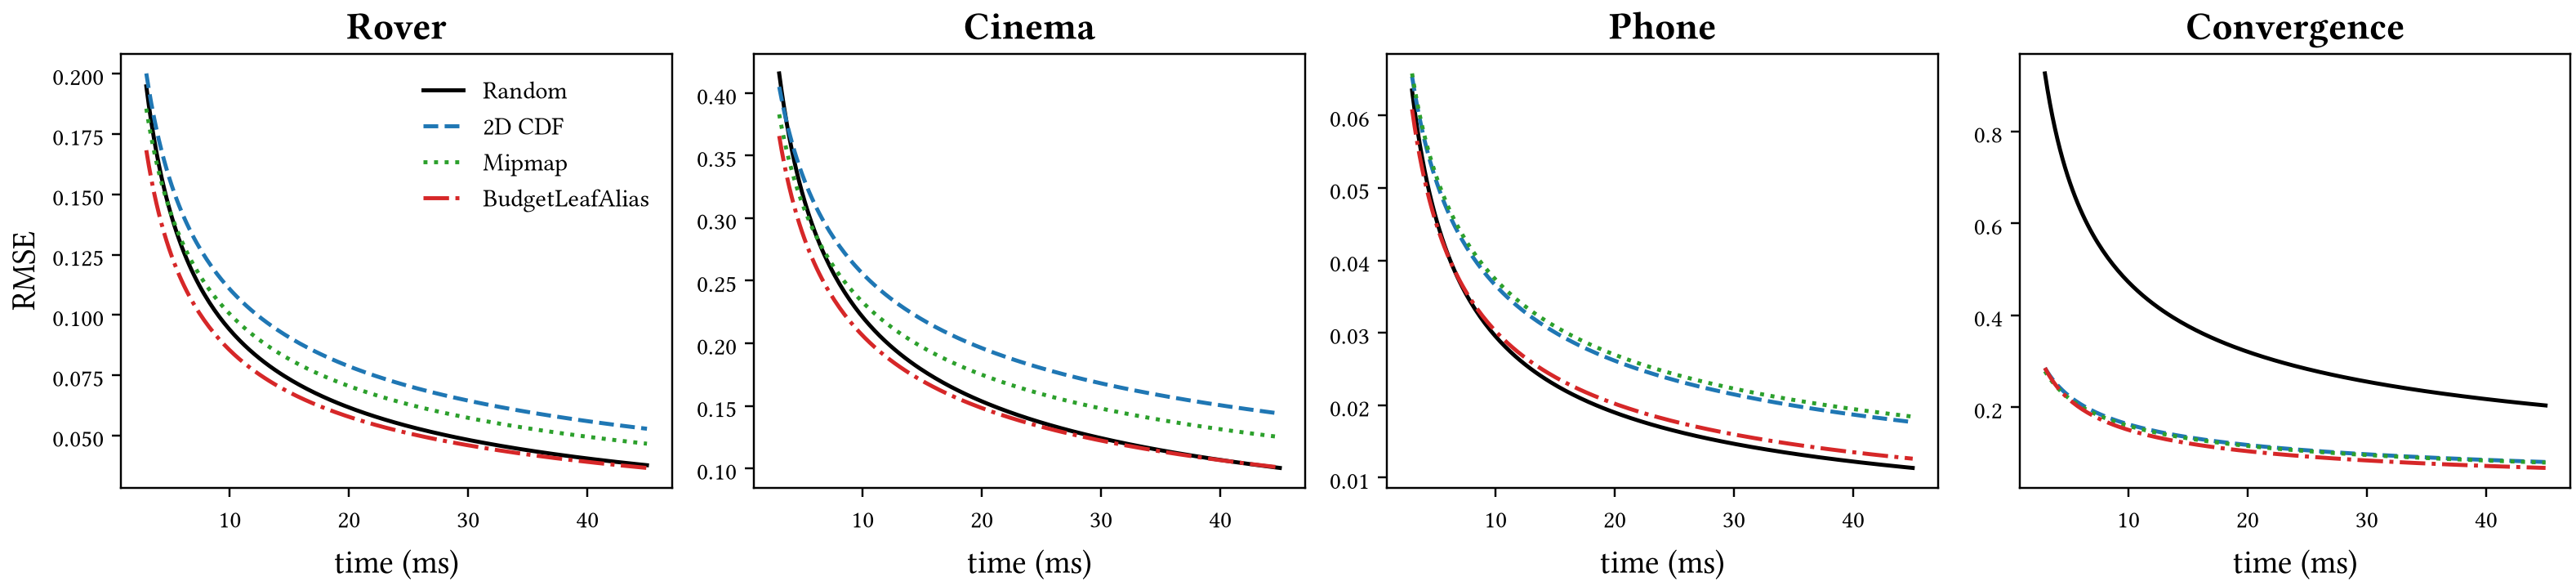
\includegraphics[width=\textwidth]{realtime_curves.png}
  \caption{Fitted RMSE-vs-time curves for Rover, Cinema, Phone, and Convergence, and all four
  techniques. BudgetLeafAlias (red) stays below both 2D CDF
  (blue) and Mipmap (green) across the entire measured range on every scene. }
  \label{fig:realtime}
\end{figure*}

\subsection{\texorpdfstring{\newt{Comparison at equal samples}}{Equal samples}}
\label{sec:equalsamples}

\newbegin
This experiment compares the techniques at the same number of samples for each scene: 4 spp and 2 light samples per vertex. We aim at measuring the variance introduced by using the LeafAlias technique. All techniques render the representative frame of each scene, 24 times with independent random numbers, and the results are compared against a converged reference (Figure~\ref{fig:equalsamples}). The three techniques that importance sample the emitter at full texel resolution (the 2D CDF, the mipmap warp and the per-pixel Alias table) reach the same error within 1\% on every scene. They sample the same distribution and differ only in how they invert it, so at equal samples, and with the independent random numbers of our renderer, they are expected to coincide. Random sampling is clearly worse: its RMSE is 1.12 and 1.21 times that of the 2D CDF on Rover and Cinema, and 1.55, 2.23 and 2.37 times on Phone, Fireplace Room and Convergence. The 2D CDF at $1/8$ resolution is up to 2.6\% behind the full-resolution techniques.

\begin{figure}[htbp!]
  \centering
  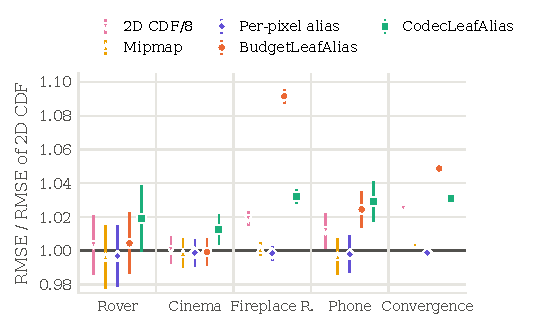
\includegraphics[width=\columnwidth]{fig_equal_samples.pdf}
  \caption{\newmat RMSE of each technique relative to the 2D CDF, with every technique using the same samples per pixel and light samples per shading point (mean of 24 renders, 95\% intervals). Random sampling, at 1.12 to 2.37, is outside the plotted range. }
  \label{fig:equalsamples}
\end{figure}

Our two techniques are slightly behind the full-resolution techniques. Relative to the 2D CDF, the RMSE of BudgetLeafAlias is $+0.4\%$ on Rover, $-0.2\%$ on Cinema, $+2.5\%$ on Phone, $+4.9\%$ on Convergence and $+9.2\%$ on Fireplace Room; that of CodecLeafAlias is $+1.2$ to $+3.3\%$ on all five scenes. The cause is the resolution of the density: both techniques choose a leaf in proportion to its mean luminance and then a point uniformly within the leaf, so the variation of luminance inside a leaf is not importance sampled. CodecLeafAlias has more and smaller leaves on such detailed content and loses less there, but its partition follows image detail rather than light, so it also spends leaves where they do not help. Figure \ref{fig:closeupsequalsamples} shows some rendering closeups for different techniques under the same number of samples.

\begin{figure}[htbp!]
  \centering
  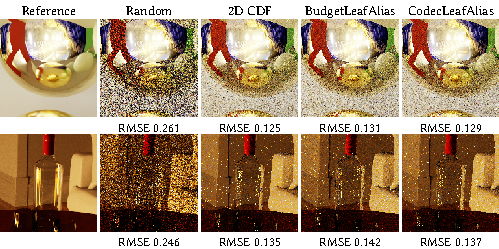
\includegraphics[width=\columnwidth]{closeup_examples.pdf}
  \caption{\newmat Examples of rendering closeups under different techniques with the same number of samples on the Convergence and Fireplace Room scenes.   }
  \label{fig:closeupsequalsamples}
\end{figure}

At equal samples, therefore, our techniques do not sample better than a texel-resolution distribution, and are not meant to: they trade a small loss of sampling quality for a much lower cost per sample and per frame.
\newend

\subsection{\texorpdfstring{\newt{Comparison at equal quality}}{Equal quality}}
\label{sec:equalquality}

\newbegin
In this experiment, we measure how long does each technique need to reach the quality that the 2D CDF delivers in real-time. 
For each scene we render the videos only with direct illumination, where the light sampler controls most of the noise. The 2D CDF uses the number of light samples that fits a 33.3\,ms frame. Every other technique is rendered with several numbers of light samples, and we find the frame time at which its video RMSE equals that of the 2D CDF. The speed-up is the frame time of the 2D CDF divided by that time.

Our two techniques reach the quality of the 2D CDF faster on all five scenes (Table~\ref{tab:equalquality}). These figures use the median frame time of each technique over several timing passes. The other techniques are not consistent: the mipmap warp is slower than the 2D CDF on Rover and does not reach its quality on Phone at the measured sample counts, and the per-pixel Alias table, which is fast on Full HD emitters, is slower than the 2D CDF on the two scenes with 4K emitters, where its memory consumption grows considerably. The time saved can be returned to the frame rate, to more bounces, or to a denoiser.

\begin{table}[htbp!]
\centering\small\newmat
\setlength{\tabcolsep}{3pt}
\caption{\newmat Speed-up of the different techniques over 2D CDF to reach the same average RMSE in the full video.}
\label{tab:equalquality}
\resizebox{\columnwidth}{!}{%
\begin{tabular}{l c c c c c}
\toprule
Technique & Rover & Cinema & Fireplace R. & Phone & Convergence \\
\midrule
2D CDF/8 & 1.17 & 1.89 & 1.29 & 1.17 & 1.17 \\
Mipmap & 0.85 & 1.45 & 1.10 & -- & 1.06 \\
Per-pixel Alias & 1.17 & 1.91 & 0.91 & 1.26 & 0.93 \\
BudgetLeafAlias & 1.31 & 2.23 & 1.19 & \textbf{1.47} & 1.27 \\
CodecLeafAlias & \textbf{1.38} & \textbf{2.31} & \textbf{1.54} & 1.23 & \textbf{1.37} \\
\bottomrule
\end{tabular}}
\end{table}

\paragraph{Emitter resolution}
The last observation suggests that the resolution of the emitter influences the advantage of our techniques. To isolate it, we render using the same emissive texture at three resolutions on the LED wall of the Rover scene: 1820$\times$1024, 3640$\times$2048 and 7280$\times$4096, obtained by area averaging from a real 8K HDR panorama of a road under broad daylight. We render frames with direct illumination, measuring time and RMSE at varying samples per pixel, and smooth the RMSE curve of each technique with a quadratic fit (Figure~\ref{fig:wall}).

\begin{figure}[htbp!]
  \centering
  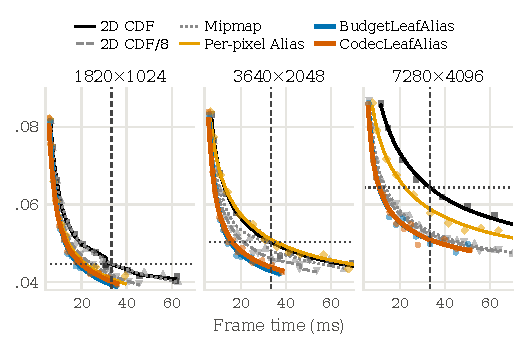
\includegraphics[width=\columnwidth]{fig_wall.pdf}
  \caption{\newmat The same image on the LED wall of the Rover scene at three resolutions: RMSE against frame time (markers: measurements; curves: fits). The vertical line is the 33.3\,ms budget and the horizontal line the RMSE of the 2D CDF at that budget. As the image grows, the curve of the 2D CDF moves to the right and ours stay almost in place.}
  \label{fig:wall}
\end{figure}

The cost of a light sample grows with resolution for the 2D CDF, and much less for our techniques. Each additional light sample per shading point adds 0.95, 1.17 and 2.93\,ms to the frame of the 2D CDF at the three resolutions, and 0.47, 0.50 and 0.73\,ms to that of BudgetLeafAlias. The 2D CDF searches a table as large as the image, with one dependent memory read per search step, and at 8K that table is sixteen times larger than at Full HD; ours read a table of about 75\,KB at any resolution, and the image only once the texel has been chosen. In a 33.3\,ms frame the 2D CDF therefore fits 34, 25 and 10 light samples, while BudgetLeafAlias fits 60, 58 and 40.

As a result, the speed-up at equal quality grows at 8K: both techniques reach the quality of the 2D CDF up to 3$\times$ faster. Read at equal time, the RMSE of BudgetLeafAlias is 12\%, 15\% and 21\% lower than the 2D CDF's. The per-pixel Alias table follows the 2D CDF, since its table also grows with the image and its memory access patterns are more incoherent. The two baselines that keep small or hierarchical structures, the 2D CDF at one eighth of the resolution and the mipmap warp, scale better and reach 2.67 and 2.44 times at 8K; they remain behind our techniques at every resolution. 
\newend

\subsection{\texorpdfstring{\newt{Sampling cost on the GPU}}{Sampling cost on the GPU}}
\label{sec:cost}

\newbegin
We relate the cost of drawing a light sample to the cache levels of the GPU with two benchmarks (Figure~\ref{fig:cache}). In the left figure, a pointer chase reads memory in a chain of dependent random accesses as the working set grows from 4\,KB to 512\,MB. It shows a sharp limit: dependent reads cost about 3\,ps (in aggregate over the whole GPU) while the data fits in the first-level cache, but three times as much once the working set exceeds 128--192\,KB, and tens of times more beyond the second-level cache (64\,MB on our GPU). 

\begin{figure}[htbp!]
  \centering
  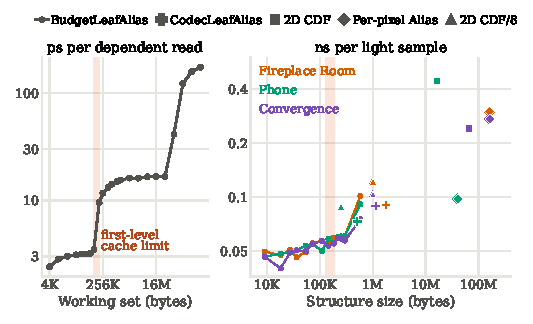
\includegraphics[width=\columnwidth]{fig_gpu_cost2.pdf}
  \caption{\newmat Left: latency of dependent random reads against the size of the data being read, on the GPU (pointer chase, aggregate over the whole GPU). Right: measured cost of one light sample against the size of the sampling structure: BudgetLeafAlias from 64 to 32000 leaves (lines), CodecLeafAlias, and the 2D CDF, per-pixel Alias and 2D CDF/8 (markers), in three scenes. }
  \label{fig:cache}
\end{figure}

In the second figure, we measure the time it takes to draw a sample and read the emissive texture, with varying $B$ values and the other techniques.
The emissive texture read is generally fast because most of the samples point to the same bright sections of the image, hence hitting cache more frequently. These results show the same behavior as the left figure. A sample of the 2D CDF costs between 0.23\,ns and 0.46\,ns, as throughput of the whole GPU, and we give the cost of the other techniques relative to it. BudgetLeafAlias at $B=4000$ is 4 to 8 times cheaper, and its cost hardly changes with the scene; CodecLeafAlias, whose table is larger, costs 1.3 to 1.6 times as much as BudgetLeafAlias. 

The per-pixel Alias table costs a quarter of the 2D CDF on the Full HD emitter of Phone, but 1.2 times as much on the 4K emitter of Convergence. This is explained by the fact that its structure, despite being $O(1)$ to sample, performs two dependent reads per sample at addresses spread uniformly over the whole structure, so almost every read misses the first-level cache; at 4K the structure exceeds the second-level cache as well, and the cost per sample more than doubles.  The 2D CDF performs 24 dependent reads per sample in the worse case, but most of them are cache hits: the marginal CDF is a few kilobytes, and the conditional searches concentrate on the few bright rows.
\newend

\subsection{\texorpdfstring{\newt{Leaf budget}}{Leaf budget}}
\label{sec:leafbudget}

\newbegin
In the next experiment, we sweep the leaf budget $B$ of BudgetLeafAlias from 16 to 16000 leaves in the five scenes at varying number of light samples per pixel. Figure~\ref{fig:leafbudget} shows the error of each budget relative to $B=4000$ at equal samples, so that only the quality of the leaf density is compared.

\begin{figure*}[htbp!]
  \centering
  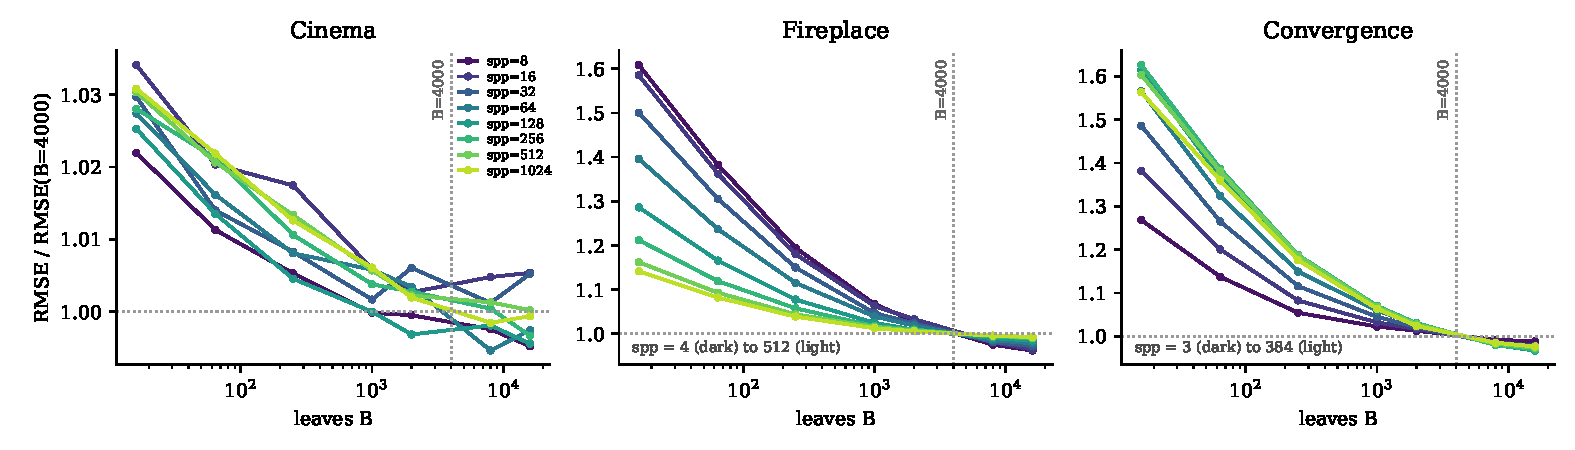
\includegraphics[width=0.92\textwidth]{fig_leaf_budget.pdf}
  \caption{\newmat RMSE against the converged reference, divided by the RMSE of $B=4000$ at the same number of light samples per pixel (spp), as a function of the leaf budget $B$. Values above 1 mean more error than $B=4000$.}
  \label{fig:leafbudget}
\end{figure*}

Two behaviors appear, depending on how the light is distributed over the emitter. In Cinema, light is spread over most of the screen, and a coarse partition already results in one figure error percentages. Rover and Phone behave in a similar way (not shown). In Fireplace Room and Convergence, most of the energy sits in small regions that the partition must resolve, and the error falls steeply with $B$ before levelling off. In Convergence, 250 leaves give up to 1.20 times the error of $B=4000$,  and 1000 leaves up to 1.07 times, while doubling or quadrupling the budget beyond 4000 improves the error by only 1--3\% at every sample count. 

On the cost side, as we saw in the previous section, the structure grows linearly with $B$, and the performance penalty is minimized as long as the sampler resides in L1 cache. $B=4000$ therefore sits at the knee of both curves: it captures nearly all the quality available from the partition, and at 75\,KB it uses most of the cache without exceeding it. $B$ acts as a memory and quality knob, and devices with smaller caches or less memory can use a smaller budget at the quality cost shown in Figure~\ref{fig:leafbudget}. All these measurements are on one GPU; the \supp{ablation\_leaf\_number} contains the complete tables and the  \supp{GPU\_tests} contain results for a mobile GPU device, showing similar patterns when using less cores and memory.
\newend



\subsection{\texorpdfstring{\newt{Frequency of frame partitions}}{Frequency of frame partitions}}
\label{sec:static}

\newbegin
As an alternative to rebuilding the partition every frame, we analyze the error generated by building the tree and leaf weights with less frequency. We compare under equal number of samples: (i)~one tree and one set of weights computed from the average of all frames, with 5\% of the probability spread uniformly to keep the estimator unbiased; (ii)~the same average tree with the weight of each leaf recomputed at each frame; (iii)~a tree rebuilt every 30 frames, with per-frame weights; and (iv)~BudgetLeafAlias. Table~\ref{tab:average-tree} reports the quality of each over the full videos.

\begin{table}[t]
\centering\small\newmat
\setlength{\tabcolsep}{4pt}
\caption{\newmat Quality for static, partially updated and per-frame trees, with 4000 leaves and equal samples per scene (samples per pixel $\times$ light samples per shading point in parentheses). The keyframe tree is rebuilt every 30 frames. The last row of each scene is the ratio of RMSE to BudgetLeafAlias, calculated before rounding. \aspnote{target values; measured now, RMSE ratio: average tree with average weights 1.02--1.40, average tree with per-frame weights 1.002--1.035, keyframe tree 1.00--1.04}}
\label{tab:average-tree}
\resizebox{\columnwidth}{!}{%
\begin{tabular}{l l c c c c}
\toprule
 &  & \shortstack{Avg. tree\\and weights} & \shortstack{Avg. tree,\\per-frame weights} & \shortstack{Keyframe tree,\\per-frame weights} & \textbf{\shortstack{Every frame\\(BudgetLeafAlias)}} \\
\midrule
\textit{Rover} & RMSE $\downarrow$ & 0.0883 & 0.0845 & 0.0842 & 0.0780 \\
(4$\times$2) & PSNR $\uparrow$ & 21.09 & 21.48 & 21.50 & 22.17 \\
 & VMAF $\uparrow$ & 71.0 & 72.0 & 72.1 & 73.4 \\
 & RMSE ratio $\downarrow$ & 1.132 & 1.083 & 1.080 & 1 \\
\midrule
\textit{Cinema} & RMSE $\downarrow$ & 0.0823 & 0.0809 & 0.0825 & 0.0748 \\
(4$\times$1) & PSNR $\uparrow$ & 22.65 & 22.80 & 22.63 & 23.48 \\
 & VMAF $\uparrow$ & 72.8 & 73.3 & 72.9 & 74.6 \\
 & RMSE ratio $\downarrow$ & 1.100 & 1.082 & 1.103 & 1 \\
\midrule
\textit{Fireplace Room} & RMSE $\downarrow$ & 0.1077 & 0.0990 & 0.1008 & 0.0905 \\
(4$\times$1) & PSNR $\uparrow$ & 19.36 & 20.09 & 19.93 & 20.87 \\
 & VMAF $\uparrow$ & 53.8 & 57.4 & 56.9 & 59.2 \\
 & RMSE ratio $\downarrow$ & 1.190 & 1.094 & 1.114 & 1 \\
\midrule
\textit{Phone} & RMSE $\downarrow$ & 0.0353 & 0.0295 & 0.0298 & 0.0272 \\
(4$\times$1) & PSNR $\uparrow$ & 29.38 & 30.93 & 30.83 & 31.63 \\
 & VMAF $\uparrow$ & 79.5 & 80.7 & 80.4 & 81.8 \\
 & RMSE ratio $\downarrow$ & 1.296 & 1.084 & 1.097 & 1 \\
\midrule
\textit{Convergence} & RMSE $\downarrow$ & 0.1866 & 0.1414 & 0.1418 & 0.1268 \\
(4$\times$4) & PSNR $\uparrow$ & 14.70 & 17.11 & 17.09 & 18.06 \\
 & VMAF $\uparrow$ & 50.3 & 60.4 & 60.2 & 62.4 \\
 & RMSE ratio $\downarrow$ & 1.472 & 1.115 & 1.118 & 1 \\
\bottomrule
\end{tabular}}
\end{table}


Rebuilding the tree and its weights every frame gives the lowest error in every scene. A fully static structure raises the RMSE by 10\% on Cinema, 13\% on Rover, 19\% on Fireplace Room, 30\% on Phone and 47\% on Convergence, where VMAF falls by 12 points: fixed weights cannot adapt to changes of the light distribution, and the uniform share spends samples on regions that are dark in a given frame. Recomputing the weights of the average tree every frame recovers most of that loss, but the fixed topology remains 8--12\% behind the per-frame tree, and a tree rebuilt once per second is 8--12\% behind as well.

These results suggest that rebuilding the partition every frame is needed, especially for dynamic content with moving bright spots like the Convergence environment map. The average tree, in addition, requires the whole video in advance, which live and streamed content does not provide, and the per-frame rebuild needs no keyframe interval and adapts at once to cuts, fades and sudden changes of light, where a stale tree is at its worst.

\paragraph{Temporal stability.} Since the partition changes from frame to frame (3--13\% of the $8{\times}8$ cells change leaf size per frame), we measured whether this introduces flicker. Appendix~\ref{app:temporal} gives the metrics and the measurements that show that the leaf density changes \emph{less} between consecutive frames than the exact per-texel density in four of the five scenes, and the low-frequency temporal error of the rendered video, the part perceived as flicker, is equal to or lower than that of the 2D CDF for BudgetLeafAlias in every scene, before and after denoising. 
\newend

\subsection{\texorpdfstring{\newt{Codec partitions}}{Codec partitions}}
\label{sec:codecstudy}

\newbegin

This section analyzes the effect of using the codec partition in CodecLeafAlias as opposed to constructing it based on a leaf number budget. 
Figure~\ref{fig:partitions} shows two examples of partitions, where the codec version is more refined in high-variance parts of the images.
To compare the partitions independently of the renderer, we compute the light-sampling variance factor of the density, $V = \sum_i f_i^2/p_i - 1$, where $f$ is the normalized luminance of the frame and $p$ the sampling density per texel; $V$ is the relative variance of a one-sample estimate of the emitter's power, and is zero for a density proportional to the frame. $V$ isolates the light-sampling part of the error and so changes far more than the rendered error.

\begin{figure}[htbp!]
  \centering
  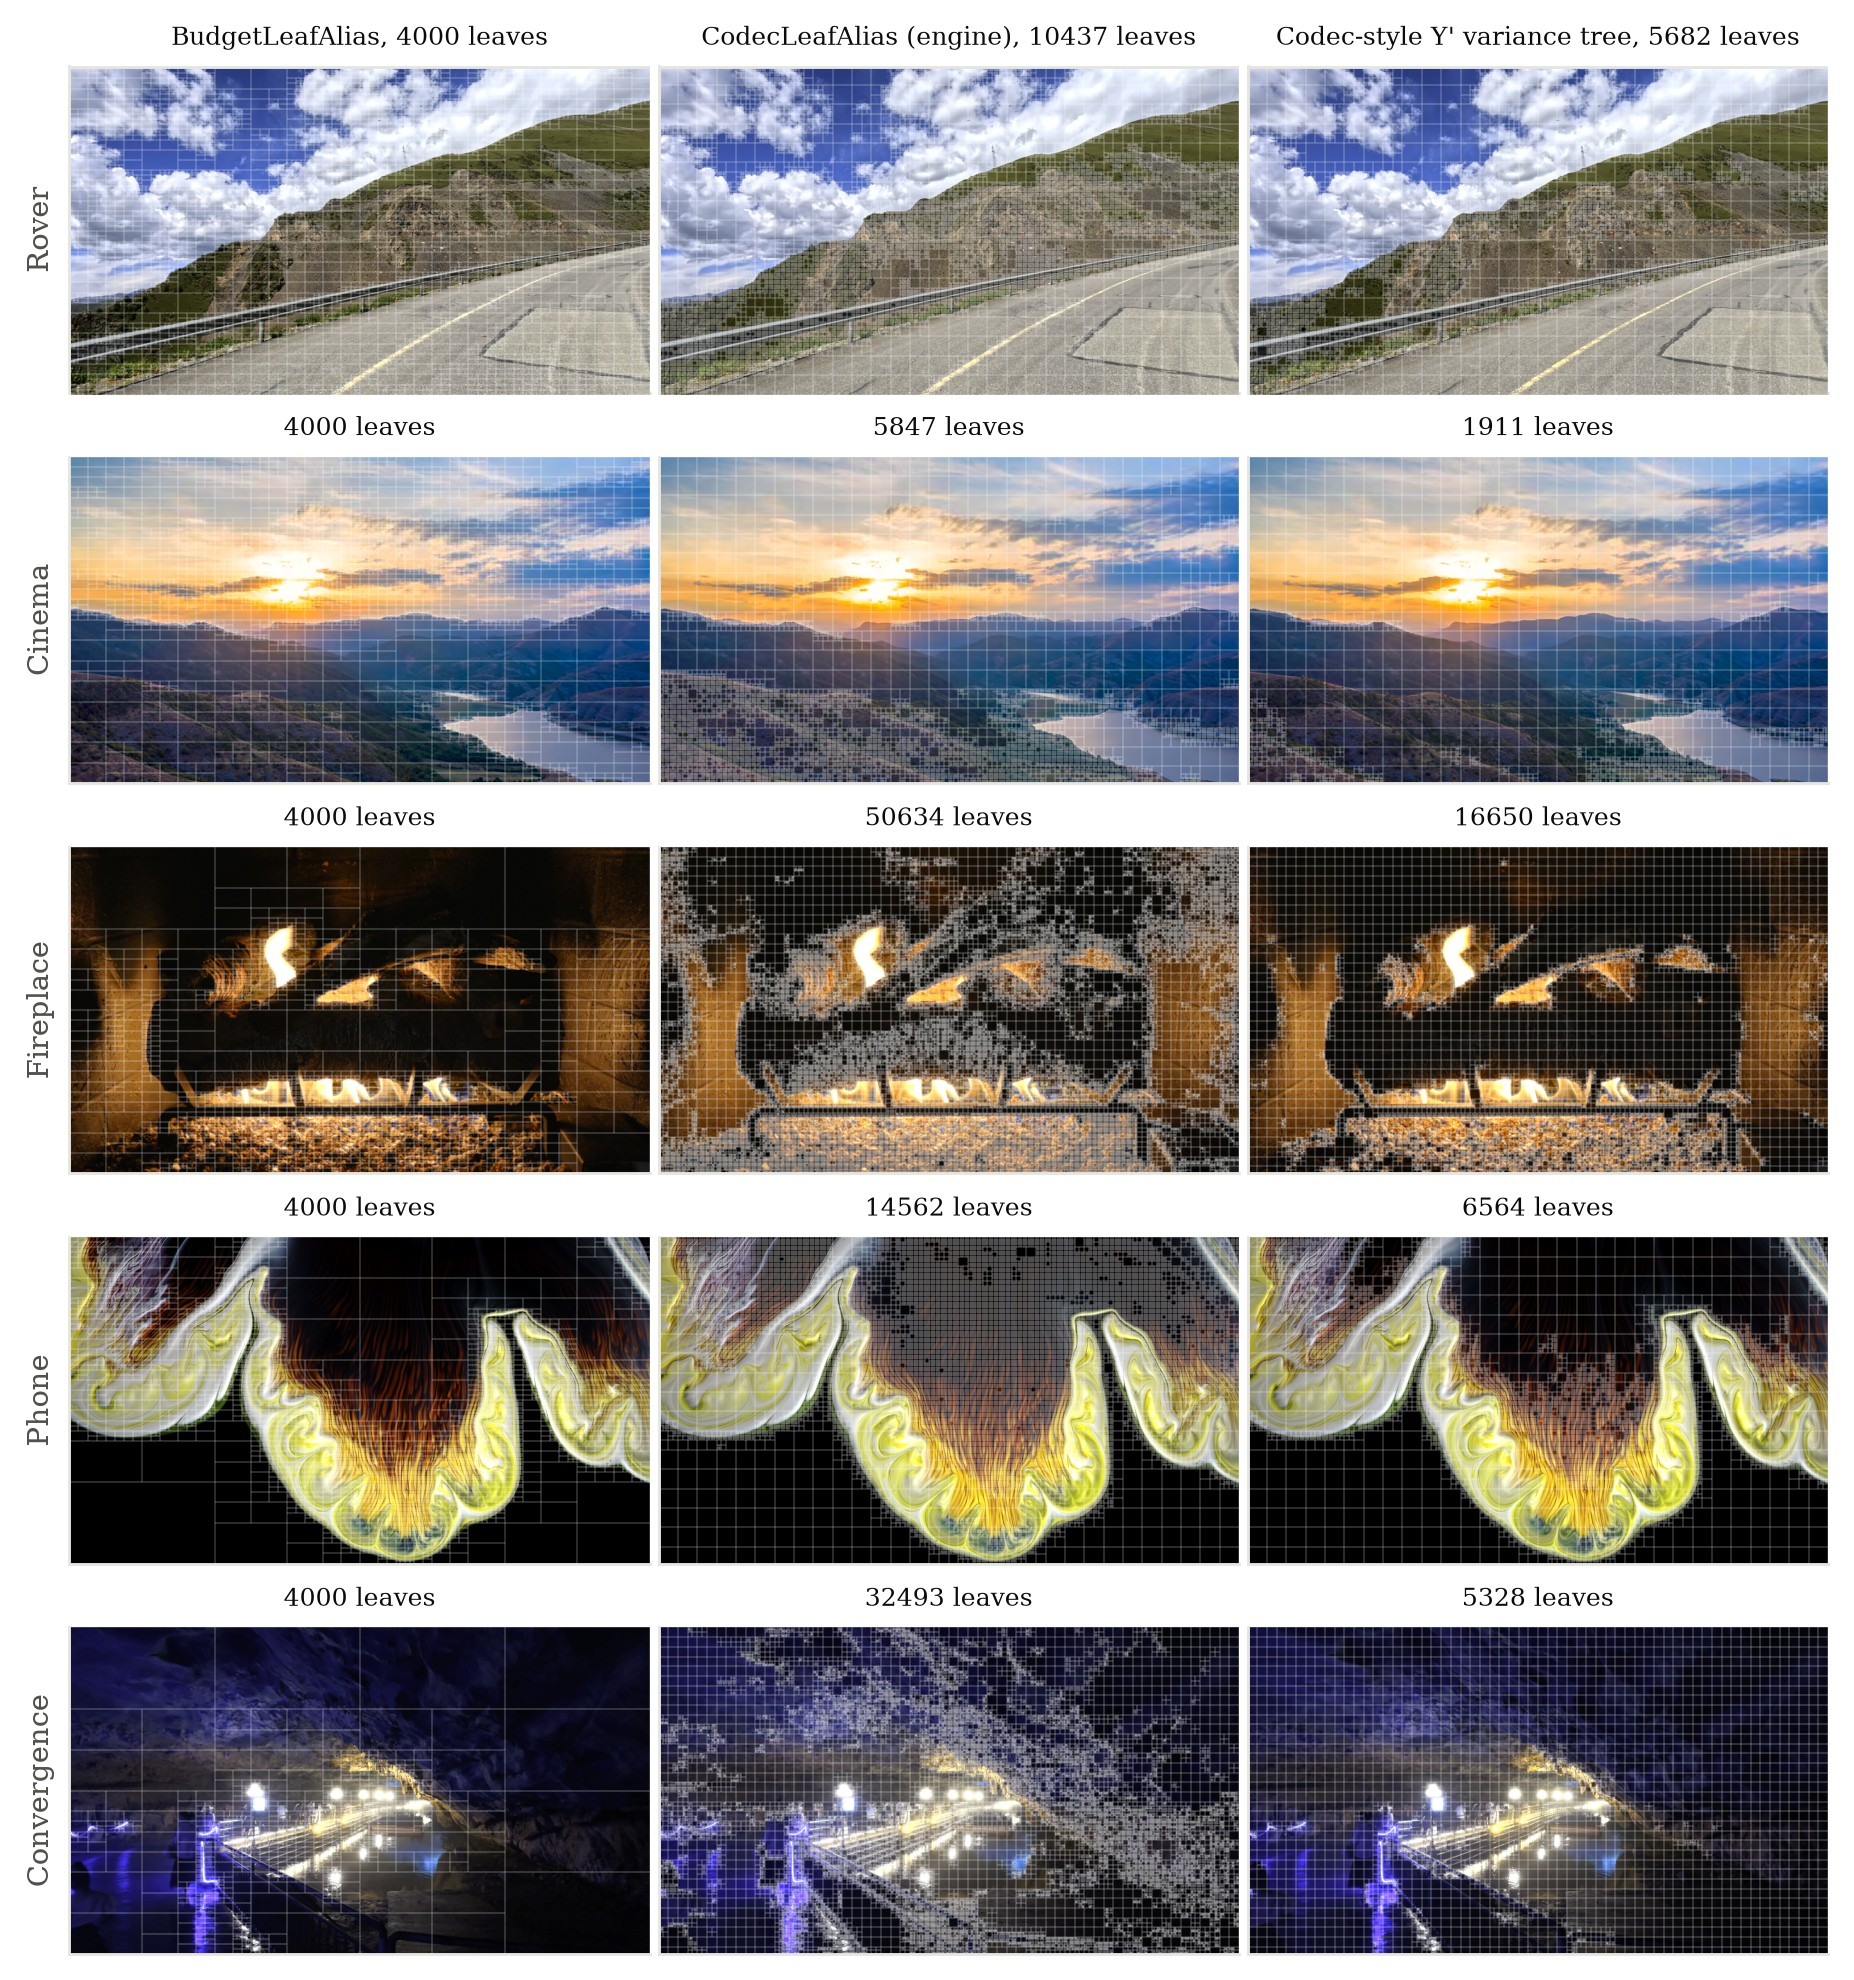
\includegraphics[width=\columnwidth]{fig_partitions.jpg}
  \caption{\newmat Leaf partitions of one frame of Rover and Phone. .}
  \label{fig:partitions}
\end{figure}

Figure~\ref{fig:variance} shows variance against leaf count for BudgetLeafAlias at varying number of leaves, and CodecLeafAlias. 
The plots show that codec leaves are placed less usefully for light sampling in every scene the codec partition lies above the budget curve, and BudgetLeafAlias reaches the same variance with 23--54\% of its leaves (94\% in Phone). A codec partition helps when it has considerably more leaves than the budget: in Fireplace Room it has about 47000 leaves, 12 times the budget, and reaches 0.26 of its variance; in Convergence about 27000 and 0.48. Rendered at equal samples, CodecLeafAlias is accordingly 5.3\% better than BudgetLeafAlias in Fireplace Room and 1.7\% better in Convergence (Figure~\ref{fig:equalsamples}), and it has the best full-video result on those two scenes (Table~\ref{tab:main}). 

\begin{figure}[htbp!]
  \centering
  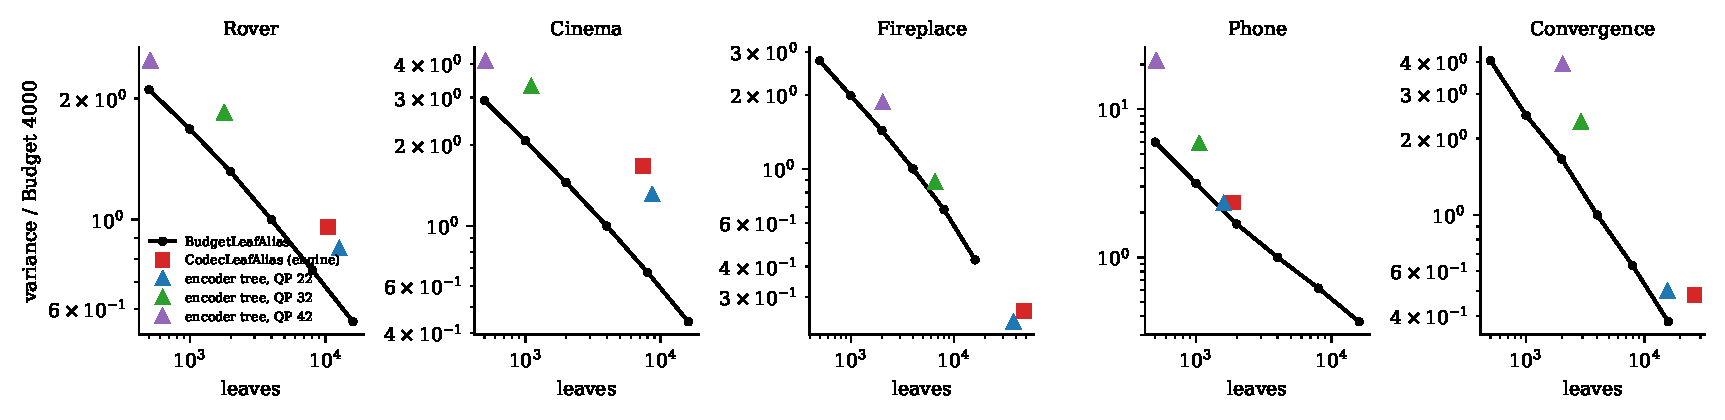
\includegraphics[width=\columnwidth]{fig_variance_vs_leaves.pdf}
  \caption{\newmat Light-sampling variance against leaf count, relative to BudgetLeafAlias with 4000 leaves (median over frames). Each line is BudgetLeafAlias from 500 to 16000 leaves in one scene, and the square of the same color is the CodecLeafAlias partition of that scene. }
  \label{fig:variance}
\end{figure}

A codec partition fails in two situations. On dark or low-contrast content the leaves go to dark detail: the Cinema partition has 7400 leaves and still 1.67 times the variance of 4000 budget leaves. And the leaf count swings with the content, by 40 times within the Phone video (528 to 20133), and with it the memory (0.2 to 2.2\,MB per frame) and the sampling cost, against a fixed 75\,KB. In summary, CodecLeafAlias is preferable when a decoded stream is at hand, the light is concentrated or the content bright and detailed, and a variable memory footprint is acceptable. BudgetLeafAlias is preferable when memory or cache size must be bounded, on dark or fading content, whenever predictable cost matters, and for emissive textures that are not decoded from a stream at all (rendered, procedural or uncompressed). The two can be combined by merging a codec partition down to a budget with the same $\mathrm{Var}\cdot A$ rule. 

\paragraph{Quantization and bitrate.}
As discussed in Section~\ref{sec:codec}, compression does not introduce bias to the estimate, so the question is how much variance it adds. We encoded the five videos in 10-bit PQ with libvpx-vp9 (CRF 12, 32, 48, 63), x265 (CRF 18, 28, 40) and SVT-AV1 (CRF 25, 40, 55), from 74 down to 0.6\,Mb/s (decoded PSNR from 51 to 32\,dB), took the leaf weights from the decoded planes as described in Section~\ref{sec:codec}, and rendered one inter-coded frame per scene at equal samples (32 captures) against the same partition with exact leaf weights.

Every ratio lies between 0.995 and 1.029 (Figure~\ref{fig:rate}), the largest PSNR loss is 0.23\,dB, and the ratios do not grow as the bitrate falls: compression error is spread over each block, while a leaf weight is the mean over the whole leaf, so most of it averages out. Taking the partition from the decoded frame instead of the source gives 0.996--1.019. Quantizing the block means directly isolates the effect of the DC quantizer: up to a step of 64 of the 1023 code values the error grows by about 3\% at most, for both partitions, and only a step of 256, a quarter of the range, reaches 4--13\%. Using the luma mean alone instead of the three planes changes the error by at most 1.5\%. 

\begin{figure}[htbp!]
  \centering
  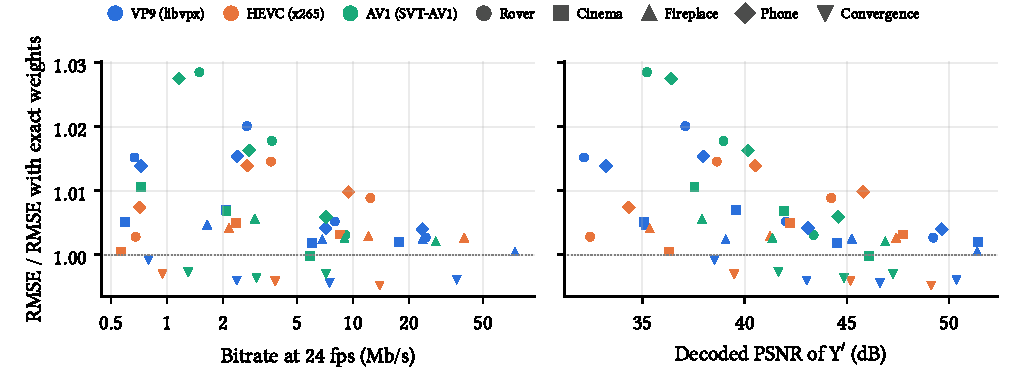
\includegraphics[width=\columnwidth]{fig_rate_sensitivity.pdf}
  \caption{\newmat RMSE of the rendered frame with leaf weights taken from lossy encodes, relative to exact leaf weights, against bitrate (left) and decoded PSNR (right), for three codecs and five scenes. All 50 points lie between 0.995 and 1.029, with no trend toward low bitrates.}
  \label{fig:rate}
\end{figure}

\paragraph{Other codecs and encoder settings.}
CodecLeafAlias needs two things from a codec: a block partition that follows image content, and the mean of each block. Every block-based codec provides the second; the first depends on the frame type. A standard configuration chooses blocks by rate-distortion (RD) search. In an intra-coded frame this splits where the image is detailed, which is what the sampler needs. In a predicted frame the search runs on the residual left after motion compensation, so its blocks follow prediction error rather than content: where motion is predicted well, a detailed region can be coded as one large block (Figure~\ref{fig:trees}).

\begin{figure}[htbp!]
  \centering
  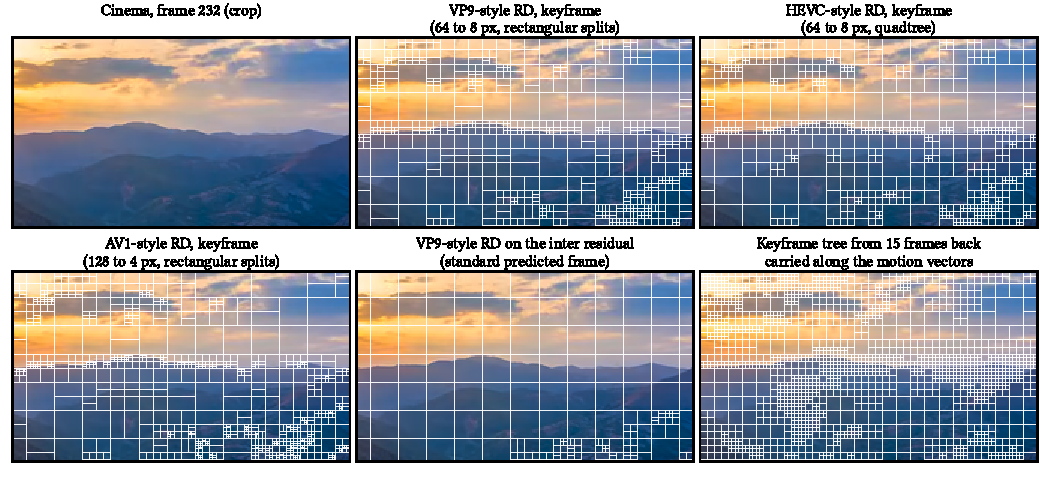
\includegraphics[width=\columnwidth]{fig_codec_trees.pdf}
  \caption{\newmat Partitions of a Cinema frame at quantizer 64 of 1023. Keyframe RD trees of the three codec families follow content. The RD tree of a predicted frame (bottom middle) follows prediction error instead and leaves most of the details in large blocks. The keyframe tree carried along the motion vectors (bottom right) follows content again.}
  \label{fig:trees}
\end{figure}

We reproduced the partition search of the three codec families on our frames, with their block sizes and split modes (VP9 and HEVC from 64 to 8 pixels, AV1 from 128 to 4), at quantizers 16, 64 and 256 of 1023, and rendered each partition with exact leaf means at equal samples. Used directly, the RD tree of a predicted frame costs up to 12\% for VP9 and HEVC and 22\% for AV1 at quantizer 64, relative to the CodecLeafAlias partition. Reusing the last keyframe's tree without moving it is better but drifts as the content moves (up to 6\%). Carrying the keyframe tree along the motion vectors of the stream, the strategy proposed in Section~\ref{sec:codec}, solves both: it stays within 2.5--4.2\% of the CodecLeafAlias partition at quantizers 16 and 64 for all three codec families, and within 5.4--6.6\% at quantizer 256, which is comparable to a partition built without any codec data. The three families behave alike for every partition source, and with weights from real encodes their worst ratios are 1.020 (VP9), 1.015 (HEVC) and 1.029 (AV1). The method is therefore tied neither to VP9 nor to its variance partitioning mode. 
\newend

\subsection{Denoised Results}
\label{sec:denoise}
Real-time renders are frequently paired with a neural denoiser in production. We pass each
technique's calibrated real-time render through the same OptiX denoiser~\cite{nvidia2021optixdenoiser} and re-measure
RMSE against the reference. Table~\ref{tab:denoise} shows that on every scene tested,
starting from our lower-noise image lets the denoiser reach a lower final RMSE than starting
from Random or 2D CDF.

\begin{table}[htbp!]
\centering
\small
\caption{RMSE before and after denoising. On every scene tested, whichever of our two techniques wins that scene keeps the lowest denoised RMSE too. }
\label{tab:denoise}
\begin{tabular}{ll cc}
\toprule
Scene & Technique & Noisy RMSE & Denoised RMSE \\
\midrule
\multirow{3}{*}{Rover}
 & Random & 0.0468 & 0.0381 \\
 & 2D CDF & 0.0779 & 0.0424 \\
 & {BudgetLeafAlias} & \textbf{0.0367} & \textbf{0.0375} \\
\midrule
\multirow{3}{*}{Cinema}
 & Random & 0.1109 & 0.0111 \\
 & 2D CDF & 0.1218 & 0.0110 \\
 & {CodecLeafAlias} & \textbf{0.0933} & \textbf{0.0106} \\
\midrule
\multirow{3}{*}{Fireplace Room}
 & Random & 0.5516 & 0.0312 \\
 & 2D CDF & 0.2295 & 0.0233 \\
 & {CodecLeafAlias} & \textbf{0.2087} & \textbf{0.0225} \\
\midrule
\multirow{3}{*}{Convergence}
 & Random & 0.3296 & 0.0148 \\
 & 2D CDF & 0.1428 & 0.0041 \\
 & {CodecLeafAlias} & \textbf{0.0870} & \textbf{0.0034} \\
\bottomrule
\end{tabular}
\end{table}


Convergence benefits the most: denoising cuts RMSE by over $95\,\%$ for every technique, and
CodecLeafAlias still finishes with the lowest denoised RMSE of the three ($0.0034$,
against $0.0041$ for 2D CDF), a direct result of feeding the denoiser a cleaner starting
image. Figure~\ref{fig:denoisedflip} additionally shows
denoised closeups and their \FLIP\  error maps for Convergence and Fireplace Room. 2D CDF's denoised output keeps a visibly brighter (higher-error) \FLIP\ map.

\new{The differences between techniques are nevertheless much smaller after denoising than before it, for two reasons. First, the denoiser removes mostly the high-frequency, per-pixel part of the error, which is precisely where light samplers differ; what remains is dominated by low-frequency residue that depends little on the number of light samples. Second, as discussed in Section~\ref{sec:equalquality}, light sampling is only one term of the error of a frame, so the room for any emission sampler is bounded before the denoiser acts. For a denoised pipeline the practical reading is the one of Section~\ref{sec:equalquality}: similar final quality is obtained from a sampler that costs less time and memory.}

Figure~\ref{fig:teaser} shows full-frame comparisons and closeups for Rover and Cinema, where
BudgetLeafAlias and CodecLeafAlias respectively remove most of the speckled noise still
visible in Random and 2D CDF's closeups. Figure~\ref{fig:figuresonly} shows
the same treatment for the remaining three scenes against a converged reference, with two matched closeups per scene; each panel also shows, in its top-left
corner, the actual HDR emissive texture that lit that scene. CodecLeafAlias visibly reduces
noise relative to both baselines.

\begin{figure*}[htbp!]
  \centering
  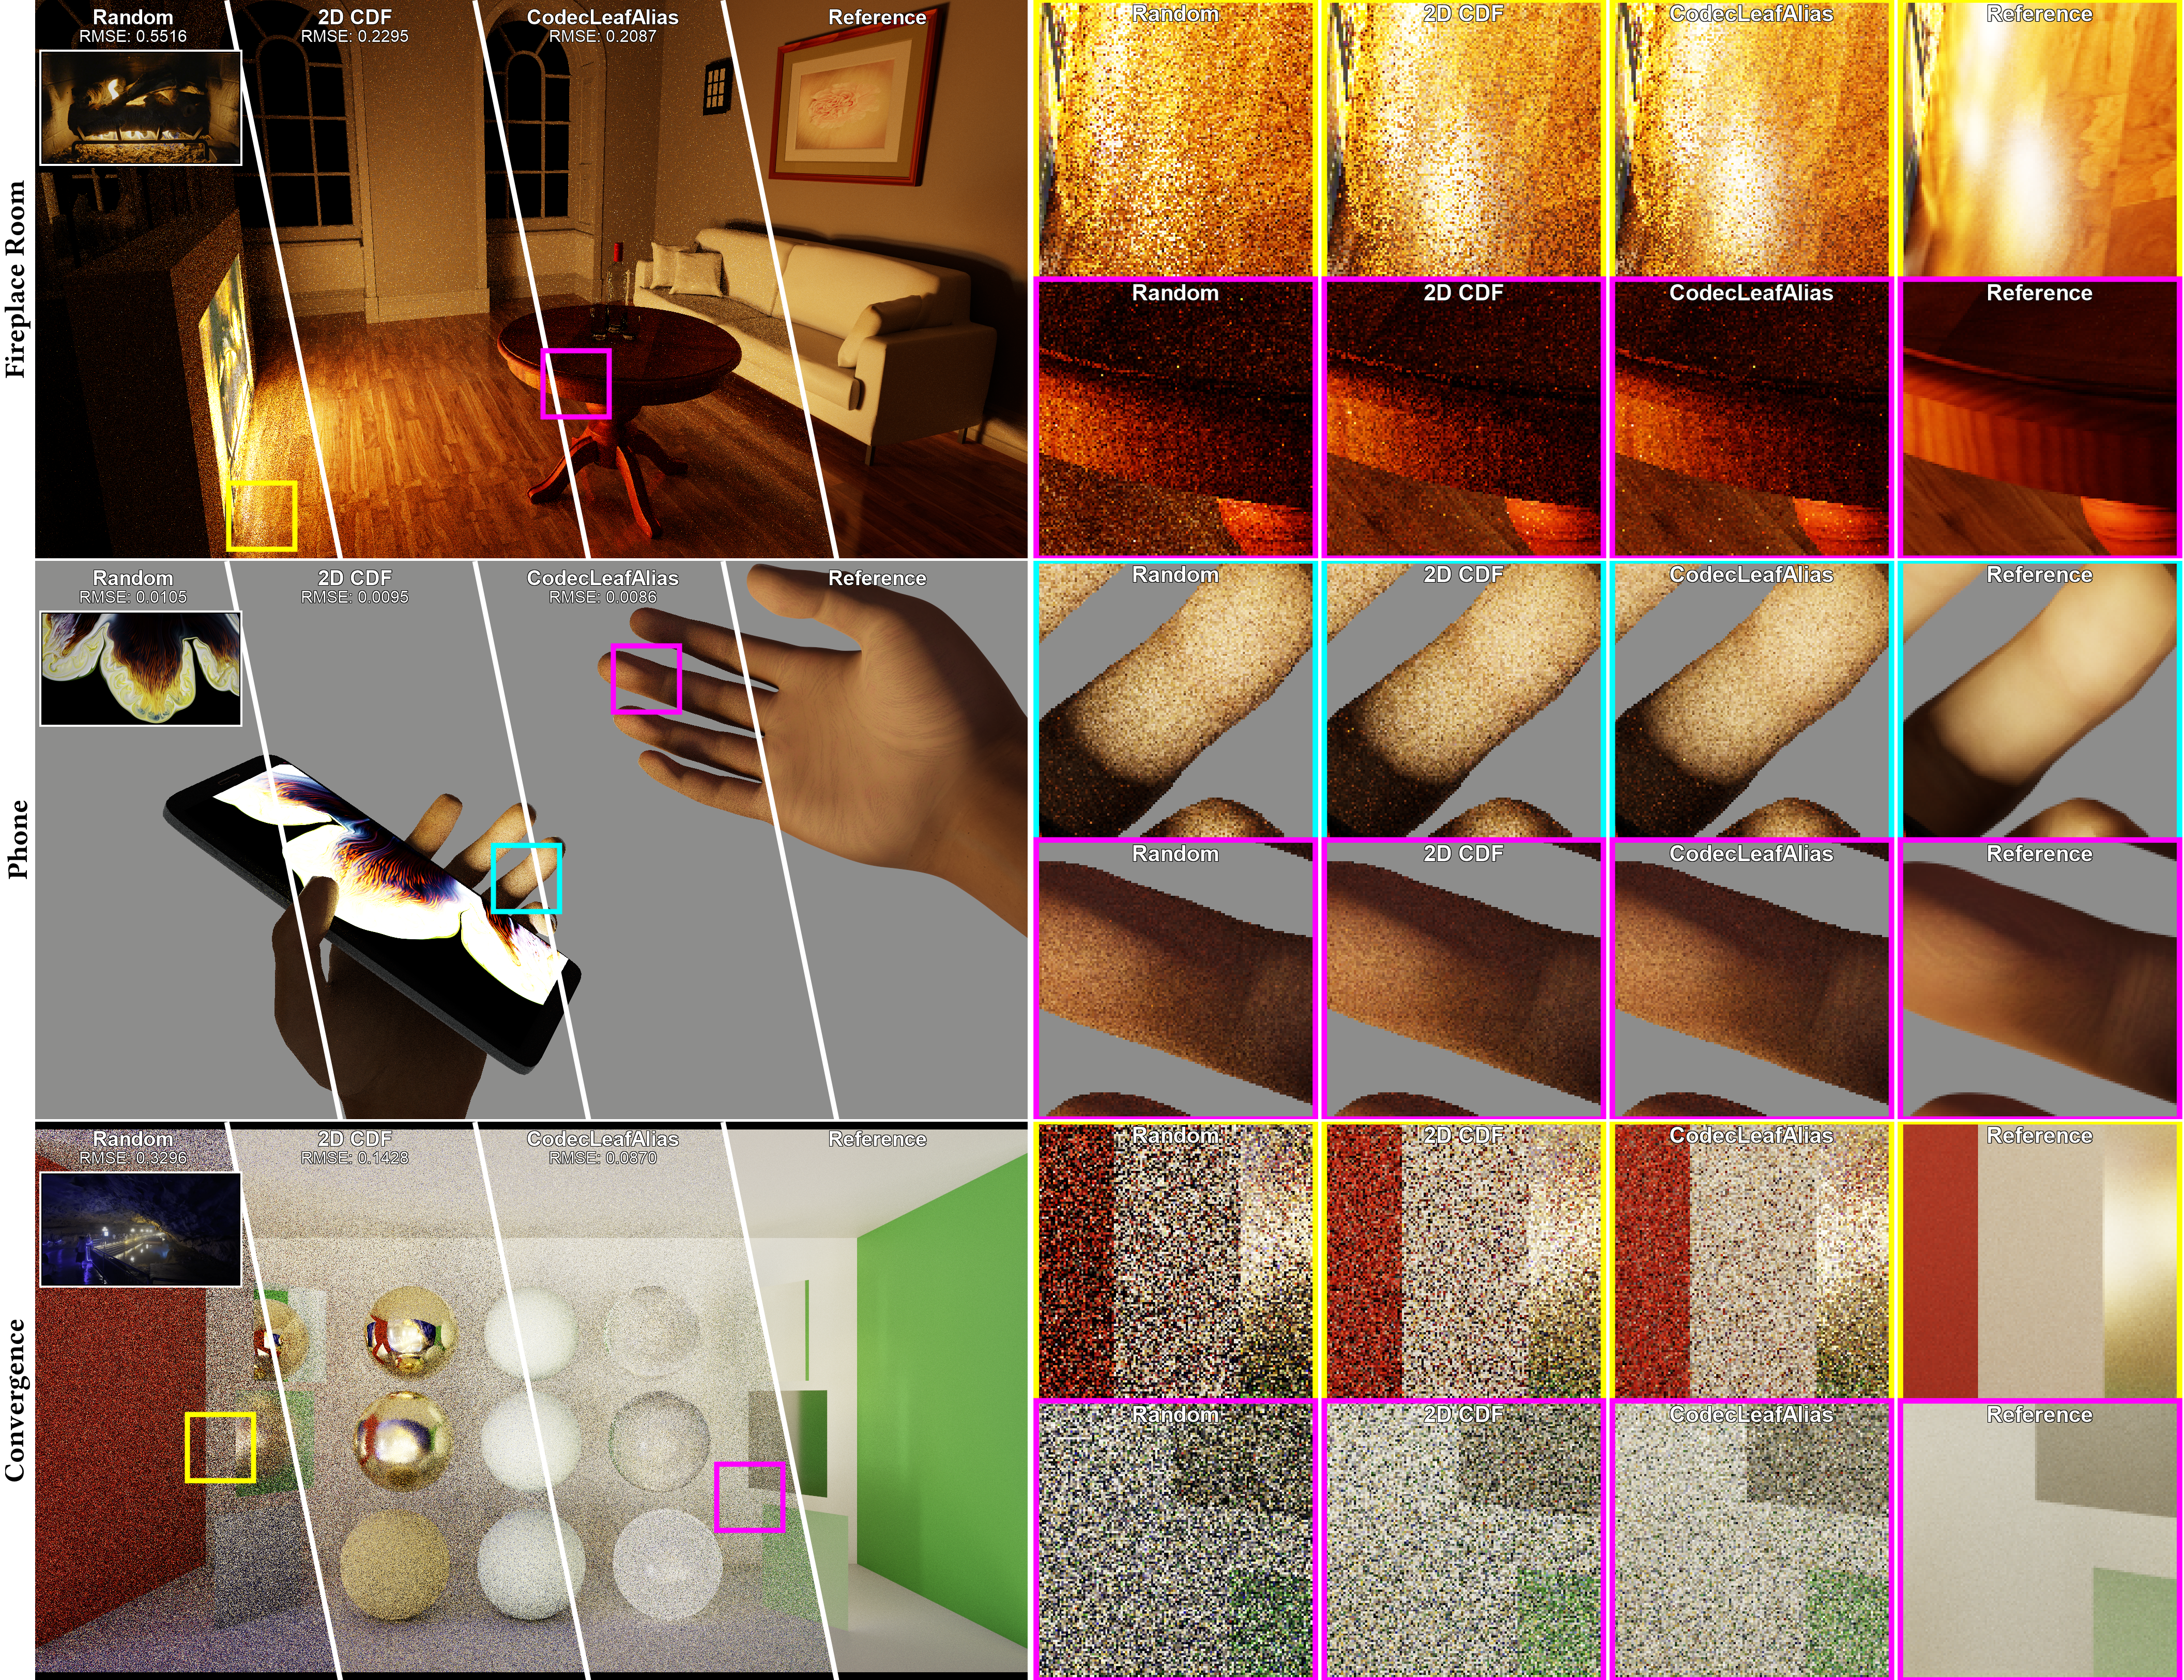
\includegraphics[width=\textwidth]{figures_only_restir_v9.png}
  \caption{Fireplace Room, Phone, and Convergence: full-frame diagonal comparisons
  (Random / 2D CDF / CodecLeafAlias / Reference) with real measured RMSE per technique, two
  large matched closeups per scene, and each scene's emissive HDR texture (top-left inset). }
  \label{fig:figuresonly}
\end{figure*}

\begin{figure*}[htbp!]
  \centering
  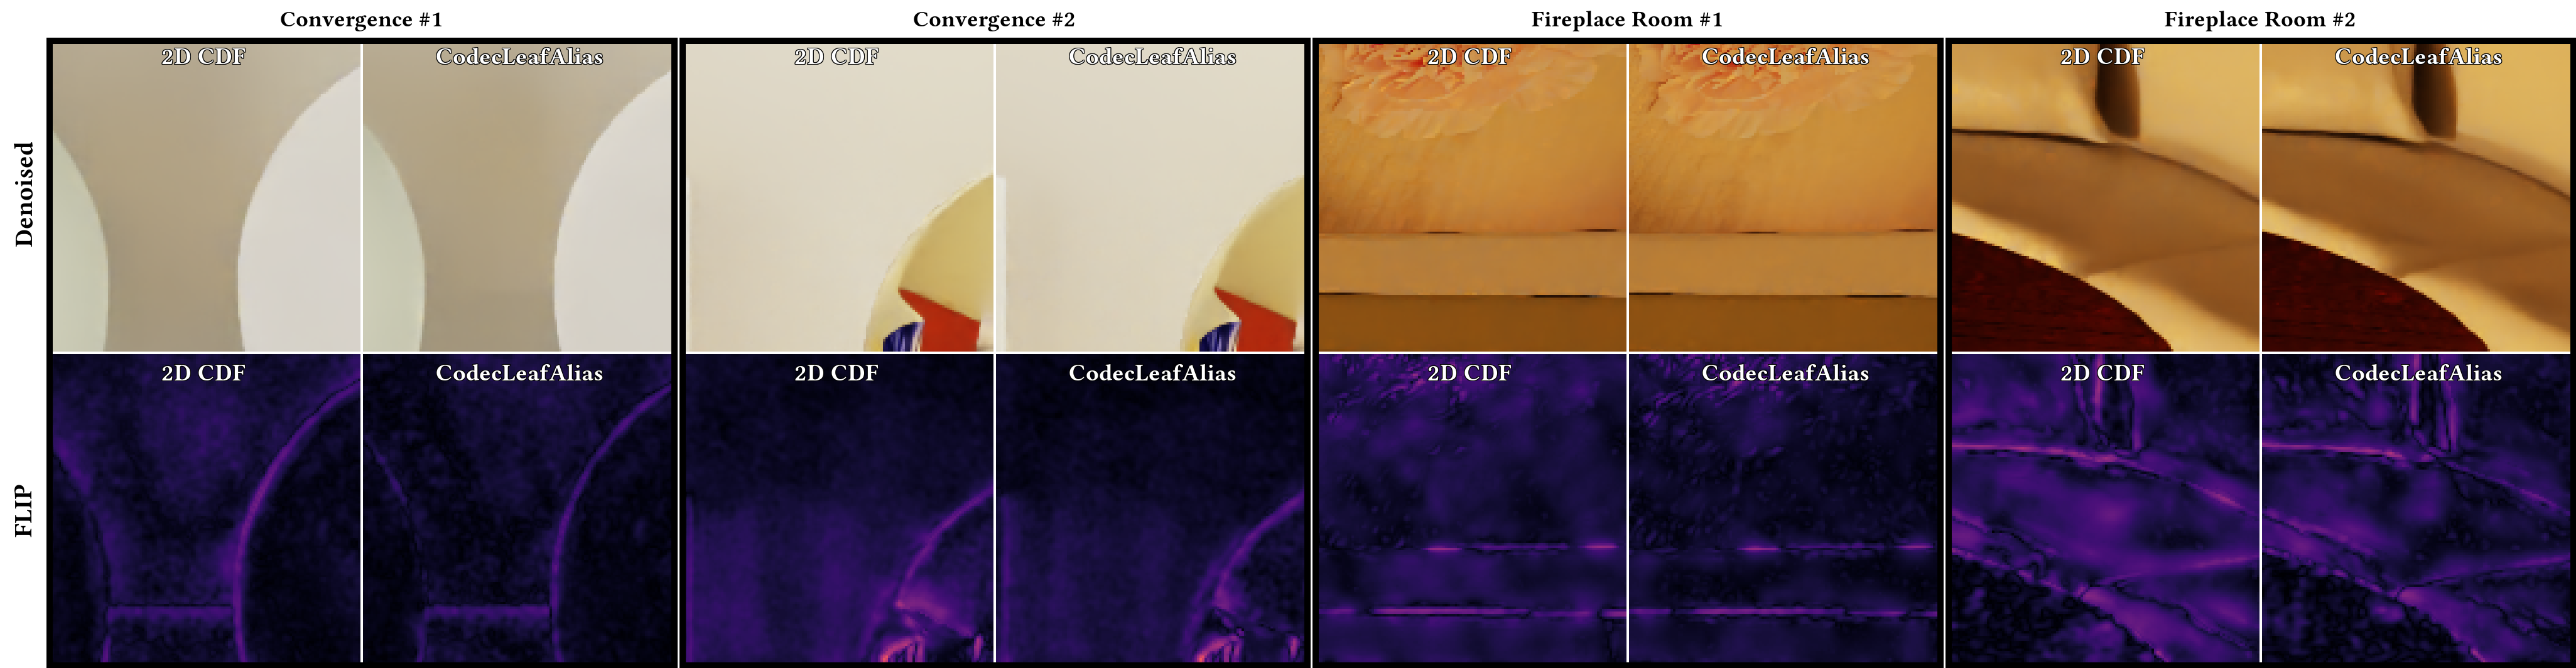
\includegraphics[width=\textwidth]{denoised_flip_grid.png}
  \caption{Denoised closeups and FLIP error maps when compared to the reference, for 2D CDF
  and CodecLeafAlias, at the two regions per scene with the largest denoised FLIP gap, for
  Convergence and Fireplace Room.}
  \label{fig:denoisedflip}
\end{figure*}

\subsection{\texorpdfstring{\newt{Discussion and limitations}}{Discussion and limitations}}
\label{sec:limits}

\newbegin
LeafAlias helps most when the sampling structure has to be small and cheap: several video lights at once, high-resolution emitters, limited memory or upload bandwidth, a tight frame, and scenes where the light sampler accounts for a large part of the error. Its limits follow from the same measurements. (i)~At equal samples it is never better than a per-texel distribution; a larger leaf budget reduces the loss. (ii)~Its gain comes from fitting more light samples in the frame, so it disappears when light sampling is a small part of the frame's cost or of its error. (iii)~It considers the texture alone: the BSDF, visibility and the distance to the emitter contribute variance that no scene-independent emission sampler removes, which bounds the gain of any such sampler. (iv)~The alias mapping does not exploit low-discrepancy sample sequences (Appendix~\ref{app:qmc}); a monotone mapping such as a 2D CDF does. (v)~Our implementation stores the mean luminance of a leaf as a 16-bit float, which saturates at 65504; emitters with brighter texels may need a wider format. (vi)~Extracting the partitions from the encoded metadata might pose some difficulty in video workflows involving hardware-accelerated decoding pipelines..
\newend

\section{Conclusions and future work} \label{sec:conclusions}

We introduced LeafAlias, a family of samplers for dynamic emissive textures that build a per-frame alias table over a variance-driven quadtree rather than over raw pixels. \rev{The outcome is a sampler that is inexpensive enough to rebuild in every frame, small enough to stay resident in the GPU's L1 cache, and accurate enough to stay within a few percent of the per-texel methods we compared against at equal samples, while reaching their quality up to 3 times faster.}

\rev{The consistency of CodecLeafAlias results through the different video light sources, codecs and bitrates that were tested suggests that the coded signal carries enough information to be reused for importance sampling. The advantage holds up when quality is judged over a full animated sequence rather than a single frame, and narrows, as for any light sampler, once a denoiser is added to the pipeline.} We also show that, when not available, building a small variance-driven quadtree is fast and can improve performance. The decision to use more or fewer leaves depends on the scene complexity and video material.

More broadly, this work points to an under-exploited overlap between the toolchains of video compression and real-time rendering. We think this connection has more to offer than the single, frame-local piece of it used here. The most direct extension is temporal. The coding-tree partition is currently extracted in every frame, discarding the motion vectors the same encoder already computes to relate consecutive frames. Since those vectors describe how the variance structure itself is moving, they could warp the previous frame's leaves into a predicted partition for the current one.
A second direction targets the leaf weights rather than the partition. CodecLeafAlias currently estimates each leaf's radiance from a single DC coefficient, which is exact under a piecewise-constant model but discards the higher-frequency information. That information could be used to guide the sampling within the leaf rectangle, potentially improving the efficiency of each drawn sample. \new{A third is the mapping itself: a hierarchical warp~\cite{clarberg2005wavelet} down the same quadtree keeps the leaf density and its small footprint, and could recover the benefit of low-discrepancy sequences that the alias mapping gives up (Appendix~\ref{app:qmc}).}

Finally, because every LeafAlias sample already carries an unbiased pdf, it composes naturally with spatiotemporal resampling: using it purely as the candidate generator inside a ReSTIR-style reservoir, rather than as the final sampler, may provide additional variance reduction on scenes with several bright, moving regions competing for the light budget.

\bibliographystyle{ACM-Reference-Format}
\bibliography{sample-base}

\appendix

\section{\texorpdfstring{\newt{Per-pixel alias tables and low-discrepancy input}}{Per-pixel alias tables and low-discrepancy input}}
\label{app:qmc}

\newbegin
The results of the paper use independent random numbers. Renderers driven by quasi-Monte Carlo (QMC) sequences expose a further difference between a per-pixel alias table and a table over leaves, which we document here. The claim is limited: LeafAlias does \emph{not} exploit low-discrepancy input; it avoids a failure of per-pixel alias tables under such input. Since the Fourier spectrum of a non-uniform sample set is not a measure of its discrepancy under the target density~\cite{li2026gradient}, we do not rely on spectra, and measure the integration error of rendered images instead.

\paragraph{How the pattern arises.}
A per-pixel alias table maps a sample $(u,v)$ to bucket $k=\lfloor un\rfloor$ of $n$ (one per texel), keeps the bucket's own texel if $v<\tau_k$ and otherwise jumps to its alias. The $N$ values of $u$ that a pixel draws from a low-discrepancy sequence are spread almost evenly over $[0,1)$, so they visit the table at a nearly constant stride of $n/N$ buckets. Vose's construction, as implemented in our renderer, lists below-mean and above-mean texels in scan order and pairs them in that order, so inside any region whose texels are all on the same side of the mean (a smooth sky, a dark hillside) consecutive buckets own consecutive texels. The constant stride through the table becomes a constant stride through the image, $H/N$ rows for an image of height $H$: when $N$ divides $H$, every sample of a pixel that falls in such a region lands in the same column. Figure~\ref{fig:qmcpoints} shows it on a $1024{\times}512$ region of the Cinema texture: the 2D CDF keeps the even spread of the Halton input, while the per-pixel alias table stacks the samples of the hillside into lines. In the spectrum of 60000 points, the strongest line is 41 times its median for the per-pixel alias table, against 1.4 for the 2D CDF and for BudgetLeafAlias. Two conditions must hold together: a stride aligned with the image rows, and long scan-order runs in the table. A textbook construction that keeps scan order everywhere, as in Figure~\ref{fig:spectrum}, produces a lattice over the whole image. Owen-scrambled sequences~\cite{owen1995randomly} randomize the stride and, in our test, remove most of the effect.

\begin{figure}[htbp!]
  \centering
  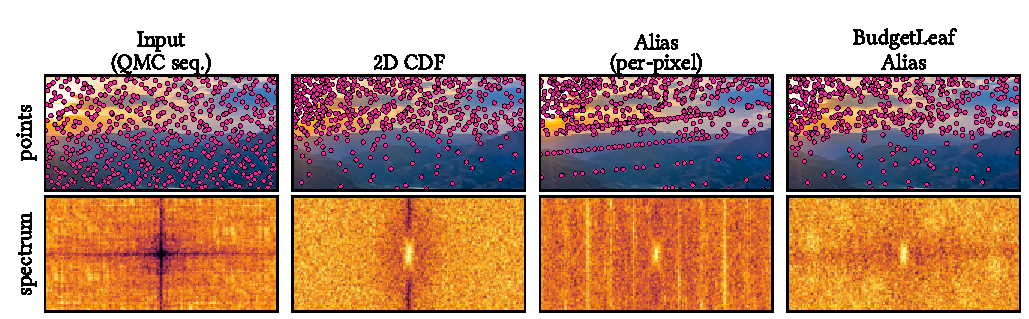
\includegraphics[width=\columnwidth]{fig_qmc_points.pdf}
  \caption{\newmat Top: the first 500 points of the Halton sequence (bases 2, 3), as input and after each warp, over a $1024{\times}512$ region of the Cinema texture. Bottom: power spectrum of the first 60000 points. The per-pixel alias table uses the table construction of our renderer; BudgetLeafAlias uses 4000 leaves.}
  \label{fig:qmcpoints}
\end{figure}

\paragraph{What it costs in a rendering.}
We render a diffuse floor lit by the textured area light through a fence (direct lighting, light sampling only, no MIS), with the Halton set and an independent toroidal shift per pixel, against an exact reference obtained by quadrature over the emitter (Figure~\ref{fig:qmcfence}, Table~\ref{tab:qmc}). With pseudorandom numbers the samplers are equal, as their densities predict. With QMC input the 2D CDF becomes 3.5 times better and the per-pixel alias table 2.6 times \emph{worse}, while LeafAlias stays at its pseudorandom level. The per-pixel alias table with QMC does not converge at all between 128 and 512 samples per pixel, where the stride is 4, 2 and 1 rows (relative RMSE 0.145 and 0.143 on the unoccluded part of the floor, against 0.054 and 0.025 for LeafAlias and 0.013 and 0.004 for the 2D CDF), and starts to fall only at 1024 samples.

\begin{figure}[htbp!]
  \centering
  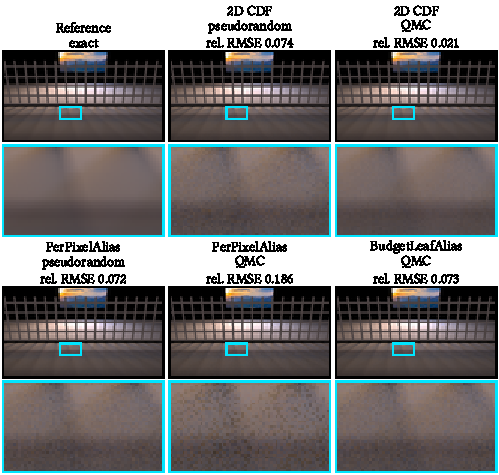
\includegraphics[width=0.92\columnwidth]{fig_qmc_fence.pdf}
  \caption{\newmat A diffuse floor lit through a fence by the emitter of Figure~\ref{fig:qmcpoints}, at 128 samples per pixel: exact reference; 2D CDF with pseudorandom and QMC input; per-pixel alias table with pseudorandom and QMC input; BudgetLeafAlias with QMC input. Close-ups below each render.}
  \label{fig:qmcfence}
\end{figure}

\begin{table}[htbp!]
\centering\small\newmat
\caption{\newmat Top: relative RMSE of the scene of Figure~\ref{fig:qmcfence} at 128 samples per pixel. Bottom: ratio of the QMC error to the sampler's own pseudorandom error over 2406 emitters and emitter regions (photographs, video frames, sky images and windows of our textures), one shading point behind six kinds of occluder.}
\label{tab:qmc}
\begin{tabular}{lcc}
\toprule
Relative RMSE, 128 spp & Pseudorandom & QMC \\
\midrule
2D CDF & 0.074 & 0.021 \\
Per-pixel Alias & 0.072 & 0.186 \\
BudgetLeafAlias (4000 leaves) & 0.074 & 0.073 \\
LeafAlias (1000 leaves) & 0.075 & 0.072 \\
\midrule
QMC error / own pseudorandom & 128 spp & 1024 spp \\
\midrule
Per-pixel Alias, median & 0.92 & 0.79 \\
\quad cases above 1.10 & 16.7\% & 7.3\% \\
\quad worst case & 1.85 & 3.51 \\
BudgetLeafAlias, median & 0.99 & 0.93 \\
\quad cases above 1.10 & 0.0\% & 0.5\% \\
\quad worst case & 1.10 & 1.20 \\
\bottomrule
\end{tabular}
\end{table}

This is not a property of one region: of 225 overlapping $1024{\times}512$ windows of the same frame, the per-pixel alias table with QMC is worse than with pseudorandom numbers in 131, and it is worse in 65\% of the 40 flat sky photographs we tested. Over 2406 emitters (Table~\ref{tab:qmc}, bottom), the QMC error of BudgetLeafAlias stays within 10\% of its own pseudorandom error in more than 99\% of the cases, whereas the per-pixel alias table exceeds that bound in 7--17\% of the cases and reaches 3.5 times. These magnitudes are a best case for QMC, a single two-dimensional direct-lighting integral; in a full path tracer both the gain of the 2D CDF and the loss of the per-pixel alias table are smaller.

\paragraph{Scope.}
A table over a few thousand leaves, each covering many texels, has no fixed relation between bucket stride and image position, so it creates no pattern; but it does not preserve the low-discrepancy distribution either, and its QMC and pseudorandom errors are the same. The 2D CDF and hierarchical warps do preserve it, at the memory and per-sample cost reported in Section~\ref{sec:cost}, and the 2D CDF remains the lowest-error sampler under QMC when that cost is not a concern. On emitters that do not trigger the pattern, among them the five videos of this paper, the per-pixel alias table with QMC input had lower error than LeafAlias. The advantage of LeafAlias here is predictability: its error does not depend on whether the pattern conditions are met. The \supp{qmc\_note}, with its code, reproduces these figures and tables and adds a convergence study.
\newend

\section{\texorpdfstring{\newt{Temporal stability}}{Temporal stability}}
\label{app:temporal}

\newbegin
We evaluate temporal stability on 60 consecutive frames of each scene, rendered at equal samples with a new random seed every frame, against a converged reference for every frame. With $I_t$ the render and $R_t$ the reference of frame $t$, the \emph{temporal error} is
\begin{equation}
E_T = \sqrt{\left\langle\left[(I_t - I_{t-1}) - (R_t - R_{t-1})\right]^2\right\rangle},
\end{equation}
averaged over pixels and frames: subtracting the reference's own change removes what the video itself does, so only change introduced by the renderer remains. The \emph{low-frequency temporal error} is the same quantity after a Gaussian blur with $\sigma = 8$ pixels, which averages out per-pixel noise and keeps the kind of change that is seen as flicker, regions pulsing or popping between frames. Independently of rendering, we measure how much the sampling density changes between consecutive frames with the Jensen--Shannon divergence.

\paragraph{The coarser density changes less.} A per-texel density follows every change of the video, including compression noise, grain and small moving details. A leaf density averages each region over many texels, so these small changes largely cancel, and a leaf boundary that moves between frames only reassigns probability between neighbouring leaves of similar radiance. The density of BudgetLeafAlias changes 5.4, 2.5, 2.5 and 1.8 times less than the exact one in Rover, Cinema, Phone and Convergence, and about the same in Fireplace Room (Figure~\ref{fig:temporal}, left), even though 3--13\% of the $8{\times}8$ cells change leaf size every frame.

\begin{figure}[t]
  \centering
  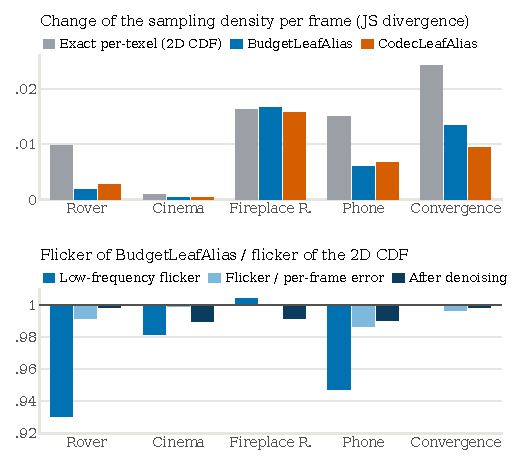
\includegraphics[width=\columnwidth]{fig_temporal.pdf}
  \caption{\newmat Top: change of the sampling density between consecutive frames, for the exact per-texel density (the 2D CDF's) and for the two LeafAlias densities. Bottom: rendered flicker of BudgetLeafAlias divided by the 2D CDF's, at equal samples; below 1 means less flicker.}
  \label{fig:temporal}
\end{figure}

\paragraph{Rendered flicker.} The low-frequency temporal error of BudgetLeafAlias is lower than the 2D CDF's in Rover, Cinema and Phone (7\%, 2\% and 5\% less) and the same in Fireplace Room and Convergence; that of CodecLeafAlias is within 0.0002 of the 2D CDF's in every scene (values of 0.0026--0.0072). The standard deviation over frames of the mean error of the whole frame (brightness pumping) is the same for all techniques. The full temporal error includes the per-pixel noise of each frame, so it grows with the per-frame error: BudgetLeafAlias is equal to or below the 2D CDF in Rover, Cinema and Phone and 4\% above it in Fireplace Room and Convergence, the two scenes where its per-frame RMSE is also 4--5\% higher. Divided by the per-frame RMSE, its temporal error is lower than the 2D CDF's in all five scenes: the partition changes add nothing measurable beyond the per-frame noise. After the OptiX denoiser, the temporal error of BudgetLeafAlias is equal to or lower than the 2D CDF's in every scene (Figure~\ref{fig:temporal}, right).

\paragraph{Frozen noise.} As a diagnostic, we also froze the random numbers (same seed every frame, no camera jitter), so that the image changes only through the video and the sampling structure. In that setting, where noise no longer hides it, the changing partition is visible as a fine-grained per-pixel change 1.5--3.6 times larger than the 2D CDF's, and a hierarchical warp over the same leaves brings it to 1.03--1.32 times. This setting does not occur in normal rendering, where a new seed every frame makes this change part of the per-frame noise, but it matters for techniques that reuse random numbers across frames, which we did not evaluate. The \supp{temporal\_stability} contains the complete tables.
\newend

\end{document}
"
\ifdefined\cleancopy\highlightfalse\fi
\ifhighlight
  \definecolor{newcolor}{RGB}{0,84,216}
  \definecolor{revcolor}{RGB}{226,106,0}
\else
  \definecolor{newcolor}{RGB}{0,0,0}
  \definecolor{revcolor}{RGB}{0,0,0}
\fi
\newcommand{\new}[1]{{\leavevmode\color{newcolor}#1}}
\newcommand{\rev}[1]{{\leavevmode\color{revcolor}#1}}
\newcommand{\newbegin}{\begingroup\color{newcolor}}
\newcommand{\newend}{\endgroup}
\newcommand{\newmat}{\color{newcolor}}
\newcommand{\revmat}{\color{revcolor}}
\DeclareRobustCommand{\newt}[1]{\textcolor{newcolor}{#1}}
\DeclareRobustCommand{\revt}[1]{\textcolor{revcolor}{#1}}
%% ---------------------------------------------------------------------------
%% Aspirational results (DRAFT ONLY): 
%%   \aspirational{text}            target text or value (magenta) followed by an [ASPIRATIONAL] tag
%%   \aspirational[note]{text}      same, with a note for whoever works on reaching the target
%%   \aspnote{note}                 the tag alone, for captions of tables and figures
%% Search this file and table_video_all.tex for "\asp" to list them.
%% ---------------------------------------------------------------------------
\definecolor{aspcolor}{RGB}{200,0,120}
\DeclareRobustCommand{\aspnote}[1]{{\leavevmode\color{aspcolor}\textsf{\bfseries[ASPIRATIONAL\if\relax\detokenize{#1}\relax\else: #1\fi]}}}
\newcommand{\aspirational}[2][]{{\leavevmode\color{aspcolor}#2}\,\aspnote{#1}}
%% Value inside a table cell: colour only, the note goes in the caption.
\newcommand{\aspcell}[1]{{\color{aspcolor}#1}}
%% Name of a document of the supplementary material.
\newcommand{\supp}[1]{supplementary document \texttt{#1}}

%%
%% The abstract is a short summary of the work to be presented in the
%% article.
\begin{abstract}
We present a method for fast importance sampling HDR textured lights that allows real-time video-driven lighting.
Our method partitions a light's texture into a budgeted, variance-driven quadtree and builds an alias table over the resulting leaves, avoiding the cost of a dense per-frame CDF while still capturing
the texture's overall energy distribution. We present two variants: one that reuses the per-frame hierarchical partitions already present in the metadata of modern video codecs, and another that builds a budgeted quadtree to fit the entire sampling structure in the L1 cache of the GPU. Compared to the dense 2D CDF-inversion baseline, at a matched real-time
frame-time budget our technique reduces RMSE by 9–53\% depending on
scene, by letting the saved sampling cost be reinvested in additional light
samples. \new{With the same number of samples, our technique doesn't introduce considerable error compared to 2D CDF, and delivers up to 3 times faster.}
It also reduces memory consumption and transfers by several orders of magnitude when compared to state-of-the-art samplers.

\end{abstract}

%%
%% The code below is generated by the tool at http://dl.acm.org/ccs.cfm.
%% Please copy and paste the code instead of the example below.
%%
\begin{CCSXML}
<ccs2012>
<concept>
<concept_id>10010147.10010371.10010382.10010385</concept_id>
<concept_desc>Computing methodologies~Image-based rendering</concept_desc>
<concept_significance>500</concept_significance>
</concept>
<concept>
<concept_id>10010147.10010371.10010395</concept_id>
<concept_desc>Computing methodologies~Image compression</concept_desc>
<concept_significance>500</concept_significance>
</concept>
<concept>
<concept_id>10010147.10010371.10010372.10010374</concept_id>
<concept_desc>Computing methodologies~Ray tracing</concept_desc>
<concept_significance>500</concept_significance>
</concept>
</ccs2012>
\end{CCSXML}

\ccsdesc[500]{Computing methodologies~Image-based rendering}
\ccsdesc[500]{Computing methodologies~Image compression}
\ccsdesc[500]{Computing methodologies~Ray tracing}

%%
%% Keywords. The author(s) should pick words that accurately describe
%% the work being presented. Separate the keywords with commas.
\keywords{Image-based lighting, video codecs, Alias tables, emissive textures, real-time rendering }

\begin{teaserfigure}
  \centering
  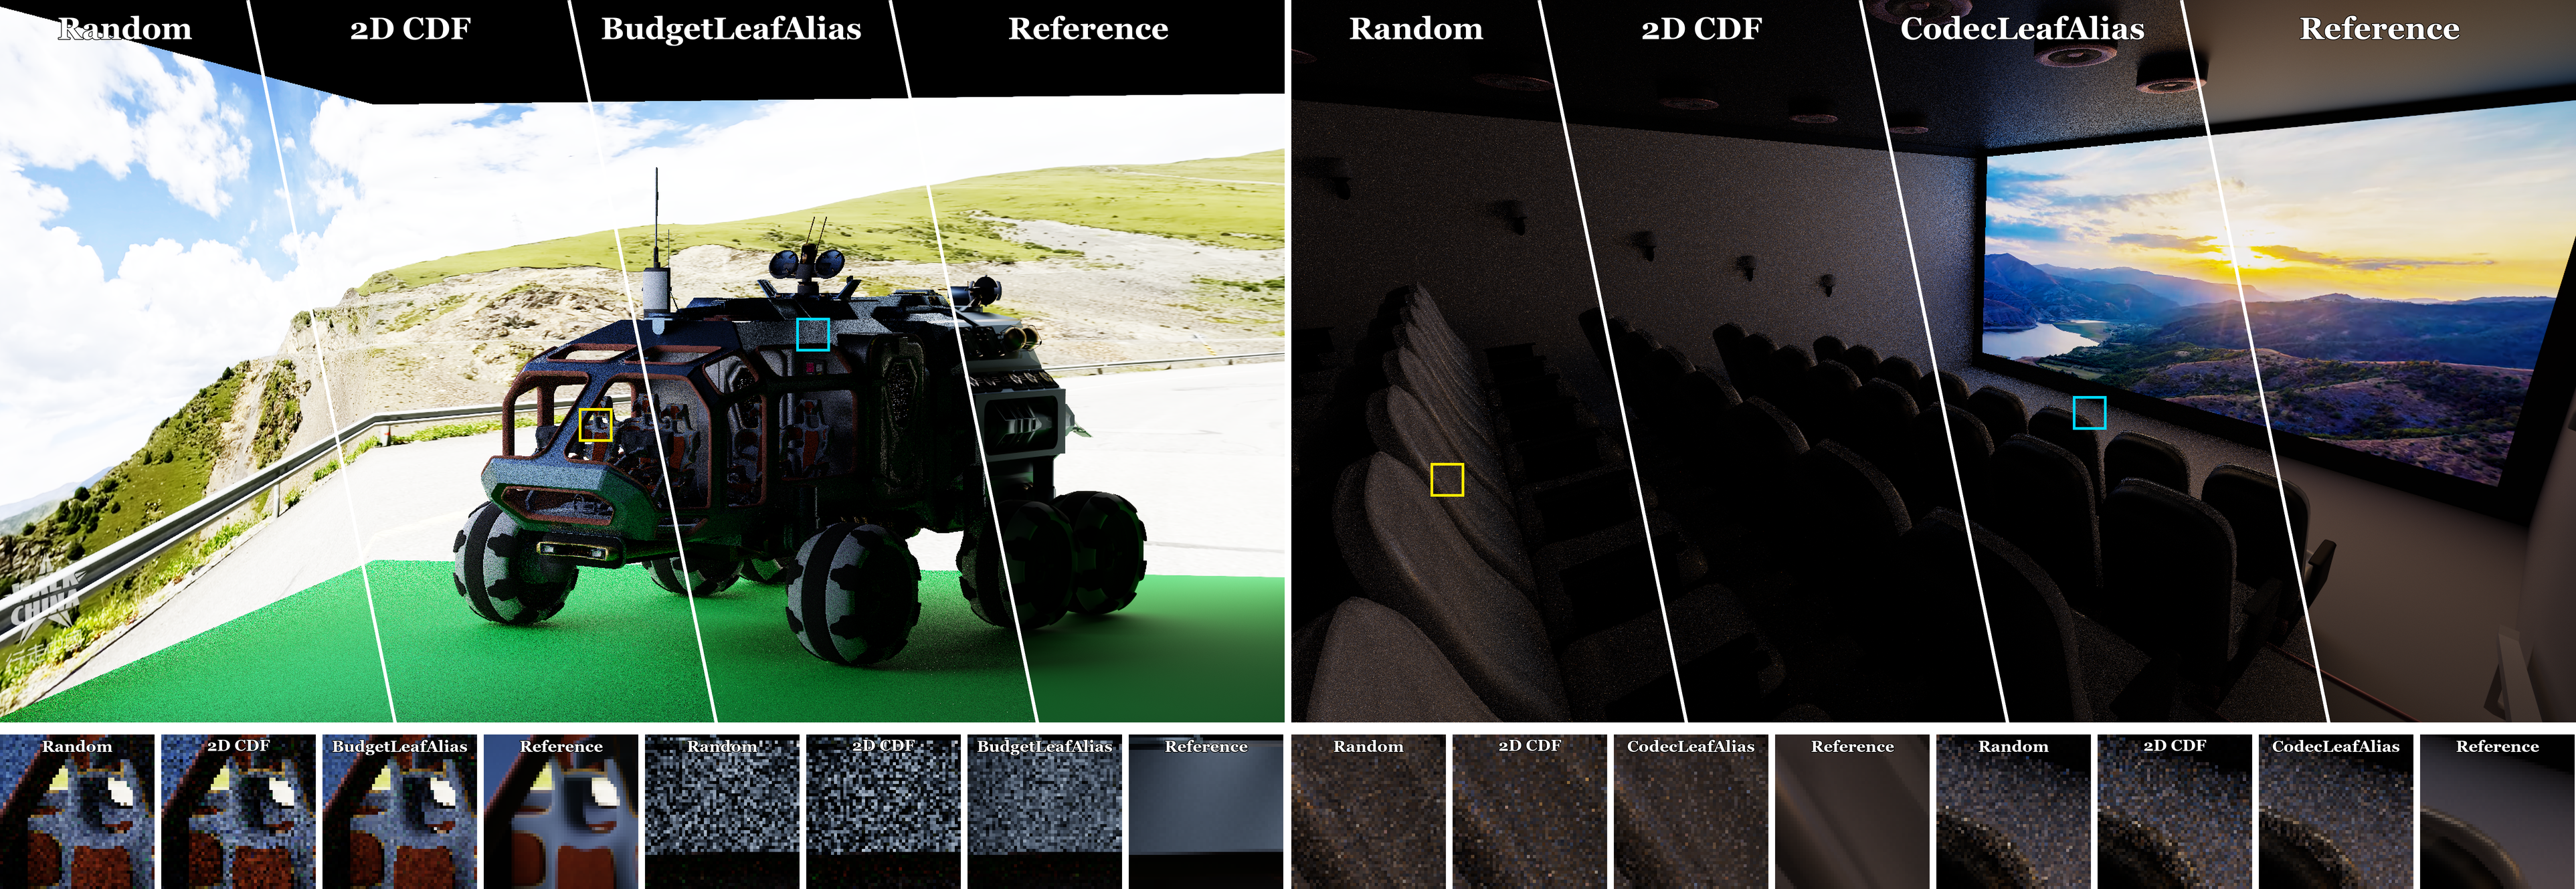
\includegraphics[width=1\textwidth]{teaser.png}
  \caption{Two scenes lit by a single dynamic, video-driven emissive texture, rendered with our LeafAlias importance sampler. (Left) The Rover scene — a virtual-production LED wall displaying a looping road/mountain video panorama that lights the vehicle directly, sampled here with BudgetLeafAlias. (Right) The Cinema scene — a theater lit only by the animated sunset footage playing on its own screen, sampled with CodecLeafAlias. Each panel compares, left to right: Random sampling, 2D CDF inversion, our technique, and a converged reference, all at their calibrated real-time budgets ($\approx$33 ms).}
  \label{fig:teaser}
\end{teaserfigure}

%%
%% This command processes the author and affiliation and title
%% information and builds the first part of the formatted document.
\maketitle

\section{Introduction}

Importance sampling of emissive textures is essential for efficient image-based lighting, and increasingly critical in production and VFX workflows where video is used directly as a dynamic light source. A single emissive texture lets a renderer reproduce the directional detail of a real environment far beyond what analytic lights can approximate. Traditionally, this texture has been static: captured once and reused for an entire sequence. However, there are recent use cases such as LED-wall virtual production, AR/VR object insertion, and video-based environment maps that require illumination that changes every frame.

\rev{The texture light samplers found in current renderers are designed for static images.} They rely on offline construction of large sampling structures that are stored and reused. The most common example of this strategy is how rendering and ray tracing toolboxes deal with HDR environment maps. The standard approach is to build a two-dimensional piecewise-constant distribution from the texture's luminance: a marginal CDF over rows and a per-row conditional CDF. The sampler is then inverted via binary search at sample time, which is expensive and produces incoherent memory access. A more recent and well-adopted approach is to generate a mipmap-style hierarchical importance map \cite{clarberg2005wavelet}. At sample time, a hierarchical descent through a mip pyramid
of the texture is performed, recursively choosing one of four children at each level in proportion to their summed weight. This technique is also expensive and requires several iterations per sample, although it is more GPU-friendly because the number of iterations is always the same for each sample, unlike with the binary search. Moreover, the mipmap can be constructed quickly using the existing dedicated hardware on modern GPUs. Both techniques require at least $O(N)$ memory for the sampler, with $N$ being the number of pixels.

Another less used but known technique for sampling emissive textures is the Alias method \cite{burke2004bidirectional}. This technique draws from an arbitrary discrete distribution in $O(1)$ time after an $O(N)$ one-time build, at the cost of losing the CDF's implicit spatial coherence: two adjacent table buckets can alias to two arbitrary, unrelated locations in the original distribution. This fact is known to disrupt stratification or discrepancy reduction of the input point set. It also requires $O(N)$ memory to store the correlation between every pixel. The process for building the Alias table, despite being $O(N)$, is difficult to optimize for real-time construction \cite{lehmann2021weighted}.

We present a new sampling method that is fast to build, produces a sampler that is tiny, \rev{is $O(1)$ to sample, and does not create the structured sample patterns that the per-pixel Alias method can produce.} The core idea is to reuse the variance-driven image partition that is already present in modern video codecs, which already compute hierarchical spatial partitions that adapt to local signal variance \cite{uhrina2024performance}. These structures implicitly encode the spatial distribution
of luminance and high-frequency content (see Fig. \ref{fig:quadtree}). We also propose a variant that builds the partition tree on a budgeted number of leaves, using a  Greedy/best-first tree-structured resource allocation strategy \cite{MINASNY2007383,Zhou2024}. \rev{Both techniques render video light textures in real time (33 milliseconds per frame) with consistent gains, because each of their samples is cheaper and more of them fit in the frame.}

\newbegin
Our samplers are per frame by design: each frame's structure is built from that frame alone, with no knowledge of past or future frames. Their purpose is not to sample a frame more accurately than an exact per-texel distribution, which is not possible, but to approach its accuracy with a structure that is orders of magnitude smaller and cheaper to build and to sample. Our contributions are:
\begin{itemize}
\item LeafAlias, an alias table over the leaves of a variance-driven partition of the texture, with $O(1)$ sampling and an $O(1)$ density lookup for multiple importance sampling, in a structure of tens of kilobytes.
\item Two sources for the partition: the coding tree of a video codec, with a study of how leaf radiance is obtained from coded data and how quantization, bitrate, codec family and encoder configuration affect it; and a greedy quadtree with a fixed leaf budget.
\item An evaluation that separates the quality of the sampling density (equal samples) from its cost (equal quality), over full videos and against per-texel baselines, together with studies of the leaf budget and its relation to the GPU cache, of static against per-frame partitions, and of temporal stability.
\end{itemize}
\newend

\begin{figure}[htbp!]
  \centering
  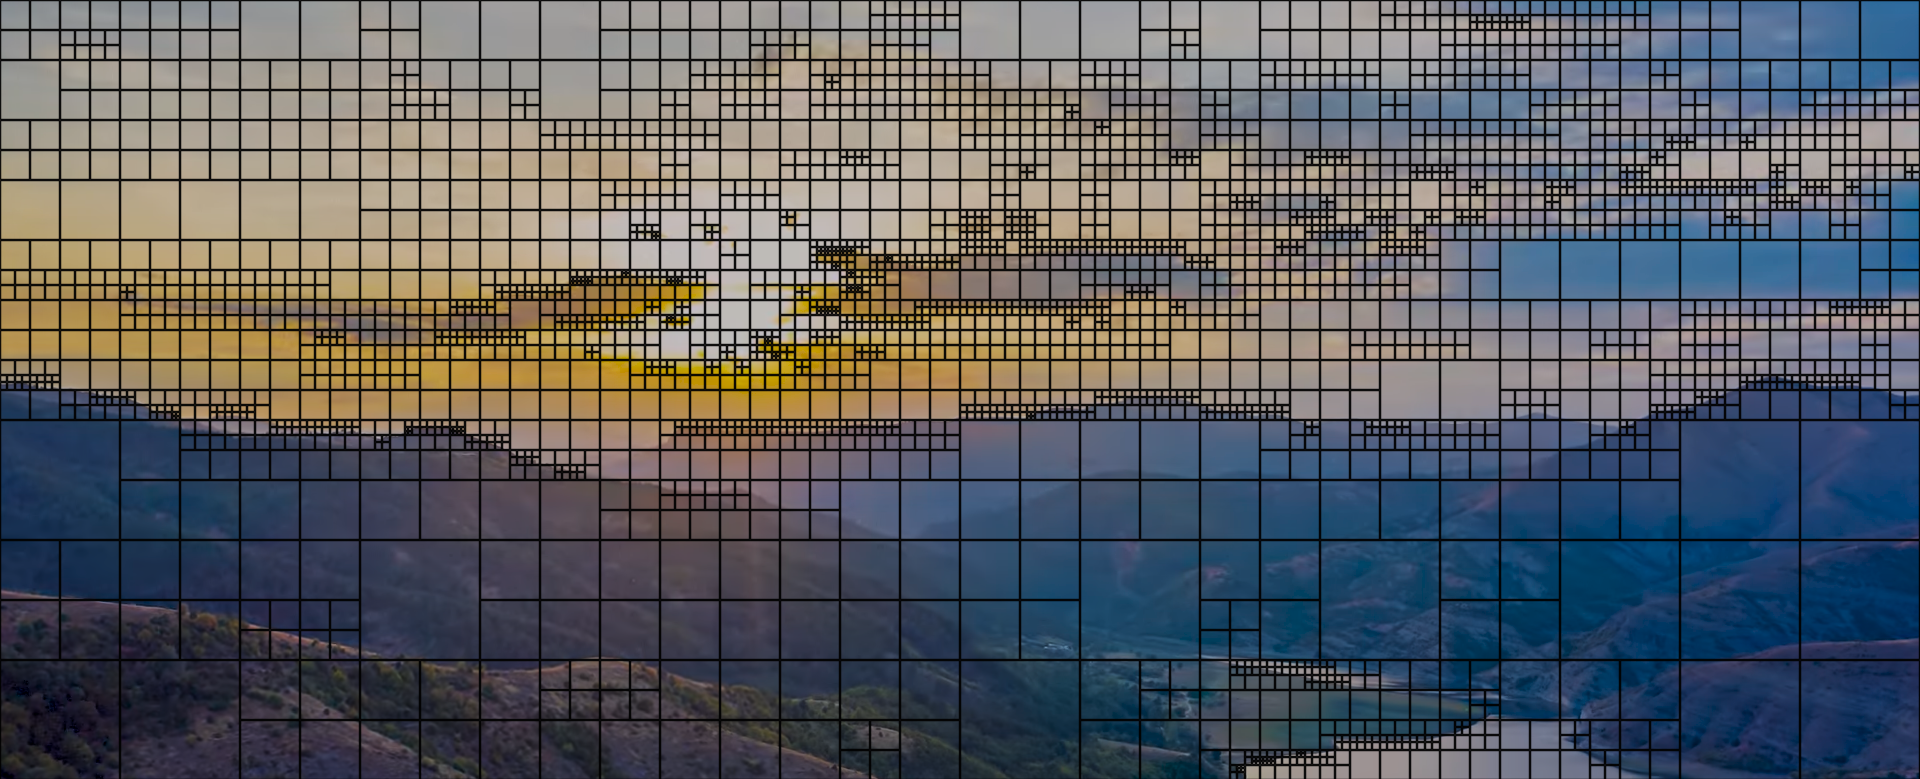
\includegraphics[width=\linewidth]{quadtree.png}
  \caption{An example of a variance-driven quadtree built by the VP9 video codec. High-variance zones are refined into a dense mesh of
  small cells.}
  \label{fig:quadtree}
\end{figure}

\new{
\section{Motivation}

\paragraph{Real-time path tracing in games.}
Light sampling with spatiotemporal resampling draws its initial candidates from
tabulated distributions over emissive geometry and environment maps
\cite{bitterli2020spatiotemporal}, and the cost of rebuilding those tables is a known
obstacle to dynamic content. Wyman and Panteleev~\cite{wyman2021rearchitecting} report the cost of
alias-table builds for large environment maps as one of the main challenges in presampling lights, and instead propose
a GPU-accelerated MIP structure to process textures coming from light probes streamed live from a 360 camera. The quality
of these initial candidates still bounds the result and limits resampling \cite{zeng2025restirpg}, and the integration
of ReSTIR in a shipped path-traced game lists initial candidate sampling quality among
its main sensitivities, with emissive surfaces and the skylight left to BSDF sampling
\cite{kozlowski2023cyberpunk}. Production engines report the same pressure from
content. Lumen lights scenes with emissive surfaces but notes how small
and bright areas cause noise artifacts, and names
explicit sampling of emissive meshes as future work \cite{wright2022lumen}; its
successor for direct lighting observes that artists now use rectangular and textured
lights more frequently \cite{narkowicz2025megalights}. Current guidance for path-traced
games recommends environment maps that are baked every frame so that dynamic skies and
clouds can be importance sampled, and a dedicated sampling structure for signs,
animated effects and procedural emissive materials \cite{nvidia2026ptwhitepaper}.
Recent work still describes the evaluation of many lights per pixel as a major
bottleneck of real-time rendering \cite{chen2026lightopt}.

\paragraph{Virtual production.}
On an LED stage the wall is at once the in-camera background and the light source of
the scene: the stage is driven as an image-based lighting instrument
\cite{debevec2022dilation,legendre2022jointly}, and the video that
drives the wall also drives the lighting fixtures around it \cite{bengtsson2022ibl}.
While the camera rolls, the panels light the real actors physically. The rendering
problem appears whenever the subject under that light is synthetic, and this happens
at three points of a production. Before the shoot, the lighting of a volume is designed
in simulation: productions go through a prelight in the virtual art department, where
the engine reproduces the environment as it will appear on the screens
\cite{kadner2023stages,zwerman2023ves}, techvis rebuilds the on-set hardware as a 3D
scene \cite{failes2024hotd}, and digitized performers are previsualized inside the
virtual stage \cite{nash2025integration}. Such previsualization of panel-generated lighting effects is older than the LED volume \cite{bunish2017rogueone,seymour2013gravity,hamon2014gravity}. During the shoot, when a shot cannot be finished
in camera, the camera frustum is keyed and provisional imagery is composited live
while the rest of the wall keeps lighting the subjects \cite{kadner2021fieldguide}.
After the shoot, the creatures and environments of such shots are added in post
\cite{failes2022hotd} and have to match the lighting that the wall gave the actors.
Research has started to treat the wall accordingly, as a near-field, high-resolution
textured emitter whose image is known at every frame \cite{azzarelli2026relightable},
and to use LED stages to reproduce per-frame HDR environment maps at video rate
\cite{zhang2026pixelcube}. In all of these cases a renderer lights a synthetic subject
with a video, and its sampling structure has to follow that video frame by frame.

\paragraph{Mixed reality and telepresence.}
In augmented and mixed reality the illumination is captured
or estimated while the application runs. HDR environment maps are inferred from the
camera feed at interactive rates on mobile devices
\cite{legendre2019deeplight,somanath2021hdr,zhao2021xihe}, estimated consistently over
video \cite{li2023spatiotemporally,shen2025stglight,bolduc2026limo}, or taken directly
from a live $360^\circ$ stream with changing real-world lights
\cite{rhee2017mr360,rhee2018mr360live,walton2018dynamic}. For such high-frequency
illumination, importance sampling of the environment map is essential for efficient
rendering \cite{kronander2015photorealistic,alhakamy2020realtime}. Systems that do
path trace under a live panorama on a head-mounted display report that the result must
be denoised \cite{cheng2023environment,wu2024panoramic}, and that in a headset Monte
Carlo noise is more than a quality problem, since its temporal flicker aggravates
cybersickness \cite{taibo2024immersive}. Most real-time systems therefore avoid
sampling: they prefilter the map or reduce it to a few dominant lights\cite{saito2024relightable}. A sampling structure that can be rebuilt at
the rate of the display, and that is small enough to keep one per light, is a
precondition for moving these applications from prefiltered shading to path tracing
with correct shadows and interreflections.
}
\section{Previous works}\label{sec:prev}
Importance sampling of emissive textures is a well-studied problem in the graphics literature in the context of image-based lighting. Most of the works focus on preprocessing the images to allow for exact or near-exact sampling without introducing bias \cite{lawrence2005adaptive}. Several methods choose to simplify the textured light into a set of point or area lights ~\cite{agarwal2003structured}, allowing for real-time sampling and faster convergence but at the cost of more error in the solution. \cite{cline2009tabular} compare several tabular inversion methods, noting the computational order of building each sampler structure and sampling each point. They analyze the 2D CDF inversion via binary search and the per-pixel Alias method, where they flag the disruption of the stratification of the input point set. \rev{With a low-discrepancy input, the raster-flattened table of the per-pixel Alias method can produce a measurable periodic banding pattern (Figure~\ref{fig:spectrum}) that becomes clear in the power spectrum of the sample set. Appendix~\ref{app:qmc} analyzes these effects and their consequence in a rendering for our proposed methods and compares it with per-pixel Alais.}

\begin{figure}[htbp!]
  \centering
  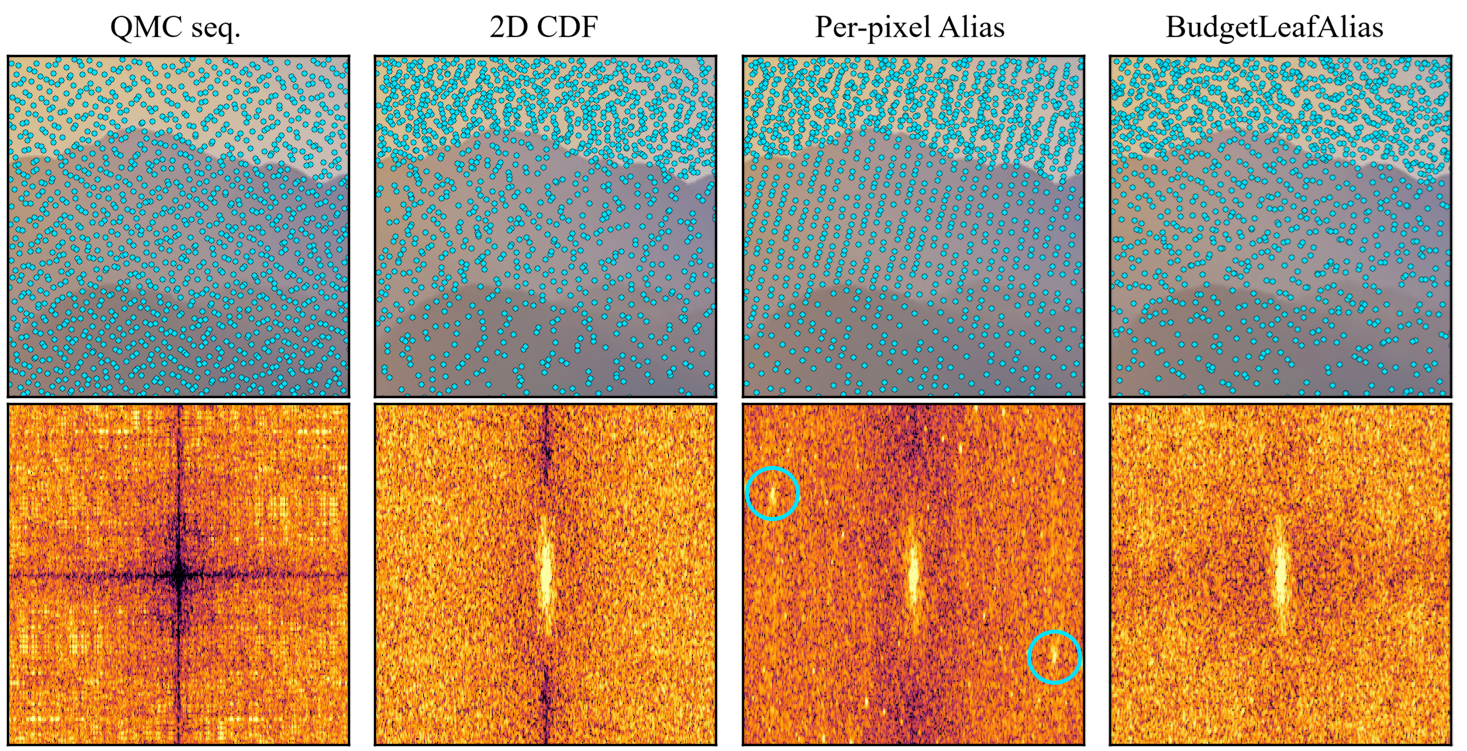
\includegraphics[width=\linewidth]{fig_spectrum_paper_color.png}
  \caption{2D power spectrum of samples from 2D CDF inversion, plain per-pixel alias, and
  our LeafAlias, from the same Halton input. Per-pixel alias shows a sharp,
  isolated off-axis peak (flatness 0.270, peak/median 16{,}113), a periodic banding
  artifact from its flat array index resonating with the input sequence's base-2 digit
  structure.}
  \label{fig:spectrum}
\end{figure}

Despite being $O(1)$ to sample, the Alias method is memory-intensive and expensive to construct via Vose's technique.
Nevertheless, it is widely used in mesh light sampling for geometry with thousands of emissive triangles. \cite{moreau2019dynamic} maintain a light-sampling BVH incrementally across frames for thousands of moving lights.
ReSTIR~\cite{bitterli2020spatiotemporal} resamples across spatial and
temporal neighbors to pick among many dynamic lights at a fraction of the cost of resampling
from scratch. Conty Estevez and Kulla~\cite{contykulla2018adaptive} adaptively split a light
tree per shading point rather than committing to one fixed cut. At that scale of thousands of triangles, a plain alias table over per-triangle flux is common practice
and cheap to rebuild every frame.

Regarding the optimization of the sampling structures,
\cite{ergun2012realtime} split an environment map into a kd-tree via the greedy partition strategy, to a predefined block count, then fit the sorted leaf probabilities with an approximate analytic curve for direct inversion. They report gains in memory compression, higher speed and accuracy than CDF inversion at matched performance for static environment maps. One disadvantage of using kd-trees is that evaluating the pdf of the map direction when sampled from the BRDF in multiple importance sampling (MIS) requires traversing the tree.
 Lambers~\cite{lambers2022parameterization} proposes a fixed-grid sampler and notes that replacing the grid with a variance-driven quadtree might improve their results. \cite{rodriguez2023nenv} train a neural normalizing flow that allows both sampling and evaluating the pdf, showing considerable performance gains at the cost of pre-training the structure for the static map. Wu~\cite{wu2025efficient} also preprocesses the map by dividing the emissive and non-emissive parts into separate structures. \new{Sz\'ecsi et al.~\cite{szecsi2010adaptive} adapt the placement of the samples of an environment map on the GPU, taking the reflectance at the shading point into account as well as the illumination. Sampling densities that depend on the shading point, like \cite{szecsi2010adaptive}, MIS-compensated distributions~\cite{karlik2019mis} or variance-aware guiding~\cite{rath2020variance}, are complementary to our work, which builds a scene-independent density from the texture alone.}

\rev{The previously described techniques focus mainly on preprocessing static images to improve sampling efficiency. Sampling of dynamic environment maps has also been studied.} \new{Wan et al.~\cite{wan2005q2tree} subdivide the sphere into a Q2-tree of quadrilaterals according to illumination importance and generate a temporally coherent set of directional samples for every frame of an environment sequence. Wan et al.~\cite{wan2011spatiotemporal} treat the whole sequence as a spatiotemporal volume and stratify the samples in space and time, and Yang et al.~\cite{yang2014high} extend this line to high-dynamic-range sequences. These methods exploit temporal coherence, and the spatiotemporal ones analyze the sequence as a whole before rendering, which suits recorded content. Our method works on the current frame only, so it applies to live video, and it produces a density that can be sampled and evaluated for MIS inside a path tracer, rather than a fixed set of light directions.} \rev{Other works address video-driven lighting:} \cite{havran2005interactive} and Iorns and Rhee~\cite{iorns2015realtime} both light scenes from captured video environment maps, but neither targets real-time per-frame
resampling of the video itself as the importance distribution. \cite{lu2013realtime} rebuild a tabulated per-cube-face CDF in real-time, noting it as an expensive part of the process. \cite{kronander2014real} rely on temporal sample reuse to improve convergence of video-based lighting.

Attempts to make the per-frame rebuild itself cheaper on a GPU point in the same direction: Morrical and Zellmann~\cite{morrical2021inverse} accelerate 2D CDF
inversion with ray tracing hardware at a high construction cost and non-trivial implementation
complexity. \cite{lehmann2021weighted} study GPU-specific weighted sampling and alias-table construction directly. \new{Binder and Keller~\cite{binder2019radix} build radix tree forests in parallel on the GPU to sample discrete distributions with a monotone mapping. These approaches make a per-texel structure faster to build; ours reduces the size of the structure instead, which lowers the cost of building it, storing it and sampling it at once.}

Modern production renderers mostly rely on dense CDF or mipmapped samplers. {Falcor}~\cite{falcorsoftware} uses a hierarchical mip-pyramid importance map over the environment texture's luminance and, separately,
the triangle-scale alias table for mesh lights. {Mitsuba 3}~\cite{nimierdavid2019mitsuba2} builds a {Hierarchical2D} warp over
the environment map, which is the same mip-pyramid family as Falcor's. {pbrt-v4}~\cite{pharr2023pbrt}
uses a dense CDF distribution, inverted via binary search. {Blender Cycles}~\cite{cyclessoftware} builds the same
kind of dense marginal/conditional CDF over a downsampled background map.

\section{Method}\label{sec:method}

The LeafAlias technique applies to any light source described by a 2D radiance texture $L(u,v)$ over
a parameter domain $(u,v)\in[0,1)^2$, e.g. an environment map, or the emission texture of an
area light. As with any textured light, variance is minimized when the sampling density
matches radiance, $p(u,v)\propto L(u,v)$. We approximate this with a piecewise-constant density
over a partition of the domain into disjoint leaf rectangles $\{R_i\}_{i=1}^N$, for now
assumed given; Sections \ref{sec:codec} and \ref{sec:budget} describe the two ways we
actually construct it. Each leaf carries a single weight proportional to its flux: its area in the parameter domain
times its average radiance:
\begin{equation}
w_i = A_i \bar{L}_i, \qquad \bar{L}_i = \frac{1}{A_i}\int_{R_i} L(u,v)\,dA. \label{eq:weight}
\end{equation}
Normalizing over all leaves gives a piecewise-constant density over the parameter domain
and a per-leaf selection probability:
\begin{equation}
p(u,v) = \frac{\bar{L}_i}{W} \ \text{for } (u,v) \in R_i, \qquad
p_i = \frac{w_i}{W}, \qquad W = \sum_{j=1}^N w_j. \label{eq:pdf}
\end{equation}
Converting $p(u,v)$ to whatever measure a particular light type actually samples with
respect to (solid angle for a distant environment map or projected solid angle for a local
area light) is a standard change-of-variables applied at evaluation time, and is
independent of the sampling structure described below.

Given the partition, we flatten it into an array of $N$ leaves, each storing its rectangle
and weight $w_i$ from Equation~\ref{eq:weight}. We build a Walker/Vose alias
table~\cite{vose1991linear} over this array once, in $O(N)$: leaves below the mean weight
are paired with leaves above it, the excess of the latter absorbs the deficit of the
former, and the process repeats until every leaf holds a threshold and, where needed, the
index of the leaf it aliases to (Algorithm~\ref{alg:build}). Unlike a dense CDF, the
resulting table needs no search at sample time since selecting a leaf is an $O(1)$ array
lookup.

\begin{algorithm}[h]
\caption{Build the alias table over $N$ leaves}
\label{alg:build}
\begin{algorithmic}[1]
\STATE $W \leftarrow \text{mean}(w_1,\dots,w_N)$
\STATE partition leaf indices into \textit{small} ($w_i < W$) and \textit{large} ($w_i \geq W$)
\WHILE{\textit{small} and \textit{large} both non-empty}
  \STATE $s \leftarrow$ pop(\textit{small}); \quad $l \leftarrow$ pop(\textit{large})
  \STATE $\mathit{threshold}[s] \leftarrow w_s / W$; \quad $\mathit{alias}[s] \leftarrow l$
  \STATE $w_l \leftarrow w_l - (W - w_s)$ \COMMENT{transfer $l$'s excess weight to $s$}
  \STATE push $l$ back onto \textit{small} or \textit{large} by its updated $w_l$
\ENDWHILE
\FOR{remaining $i$ in \textit{small} $\cup$ \textit{large}}
  \STATE $\mathit{threshold}[i] \leftarrow 1$
\ENDFOR
\end{algorithmic}
\end{algorithm}

\subsection{Sampling}
\label{sec:sampling}
To draw a light sample, we use three uniform numbers $\xi_1,\xi_2,\xi_3$
(Algorithm~\ref{alg:sample}). $\xi_1$ selects a bucket in $O(1)$;
$\xi_2$ decides whether we keep that leaf or its
alias partner.
$\xi_3$ and $f$ place the sample uniformly
inside the chosen leaf's rectangle. The sample's pdf is read directly from its
leaf's stored average luminance via Equation~\ref{eq:pdf}. Radiance is read from the texture at the sampled $(u,v)$.

\begin{algorithm}[h]
\caption{Draw one light sample}
\label{alg:sample}
\begin{algorithmic}[1]
\STATE $i \leftarrow \lfloor \xi_1 N \rfloor$; \quad $f \leftarrow \xi_1 N - i$
\IF{$\xi_2 < \mathit{threshold}[i]$}
  \STATE $\mathit{leaf} \leftarrow i$
\ELSE
  \STATE $\mathit{leaf} \leftarrow \mathit{alias}[i]$
\ENDIF
\STATE $(u,v) \leftarrow \text{lerp}(R_{\mathit{leaf}}.\mathit{min}, R_{\mathit{leaf}}.\mathit{max},\, (f,\xi_3))$
\STATE \textbf{return} $(u,v)$, $\;p(y){=}\bar{L}_{\mathit{leaf}}/W$ (Eq.~\ref{eq:pdf}), $\;L(u,v)$
\end{algorithmic}
\end{algorithm}

Combining light sampling with BRDF sampling via MIS requires the
reverse query: given a direction chosen by BRDF sampling that happens to hit the light at
some $(u,v)$, the probability $p(y)$ is needed. Rather than searching the partition, we
maintain a small auxiliary lookup matrix that maps a coarsened $(u,v)$ coordinate directly to
its leaf index, at a fixed fraction of the texture's resolution matching the partition's
smallest possible leaf (e.g.\ one entry per $8{\times}8$ block).
Every coordinate covered by a given leaf is written to the same entry at
construction time, so the lookup is an $O(1)$ array read that reproduces the exact same
$\bar{L}_i/W$ used at sampling time regardless of that leaf's actual size, keeping the
resulting MIS weight unbiased. We also tried replacing this exact lookup with a single
scene-wide average density: across our test scenes this produced no perceptible difference
in the rendered images, but it does introduce bias, since the substituted value no longer
matches the technique's actual density at that point.

\subsection{CodecLeafAlias}
\label{sec:codec}
Building the partition can be costly, especially for dynamic content that changes every few milliseconds.
CodecLeafAlias avoids it entirely when the texture
arrives as a compressed video frame. Modern codecs (HEVC, AV1, VP9) already split each frame
into a coding-tree hierarchy driven by local signal variance, which is structurally the same
partition our method needs.
We take each coding-tree leaf's block directly as one of our leaf rectangles $R_i$, and
estimate $\bar{L}_i$ from the block's own zero-frequency (DC) transform coefficient rather
than summing pixels: the DCT/DST's DC term is, up to a fixed normalization constant, exactly
the block's mean sample value, and is already computed and present in decoder metadata.
\newbegin
The DC coefficient gives the mean of a block of the \emph{coded} signal, which for HDR video is a nonlinear, quantized $Y'C_bC_r$ signal (10-bit PQ, BT.2100, in our experiments), so three steps separate it from $\bar{L}_i$. (1)~The reconstructed block mean of each plane is its dequantized DC divided by the transform gain. For a block coded with prediction, the DC belongs to the residual, and the mean of the prediction (extracted from the decoding process) must be added. (2)~The three means are converted to $R'G'B'$ with the BT.2020 matrix, linearized with the PQ transfer function, and transformed to luminance with the BT.2020 weights. (3)~The result is multiplied by the leaf area to give $w_i$ (Eq.~\ref{eq:weight}). This process and quantization perturb the DC, and therefore the density of Eq.~\ref{eq:pdf}, but not the expected value of the estimator: every sample is divided by the density actually used, so the estimate stays unbiased for any density that is positive wherever the emitter is. We keep a small density floor ($10^{-4}$ of the mean weight) so that no lit leaf is quantized to zero. A wrong weight can therefore only add variance; Section~\ref{sec:codecstudy} measures the effect of quantization in the results.
\newend

In our experiments, we encode the dynamic emissive textures as HDR video using libvpx's VP9 Profile 2 and extract the superblocks for each frame via decoder statistics. We configure the encoder to always use variance-based superblock partitioning. Encoder settings that instead search or reuse partitions (full rate-distortion search, predicted neural partitions, etc.) \new{can} still supply a usable partition by combining each block's motion vector with its keyframe's already-computed superblocks. \new{Section~\ref{sec:codecstudy} evaluates this strategy, other codec families and the effect of bitrate.} 

Using codec partitions results in varying number of leaves, ranging from 4000 to 20000 depending on the content. We call this method CodecLeafAlias. Since the sampling algorithms are memory-bound operations, we go further by defining a new partition mechanism that allows us to choose a budgeted number of leaves to reduce memory needs and improve coherence. We call this other method BudgetLeafAlias.

\subsection{BudgetLeafAlias}
\label{sec:budget}
BudgetLeafAlias constructs the quadtree directly from the texture under a hard
leaf-count budget $B$ (in our implementation, matched to what fits alongside the alias
table in a modern GPU's L1 data cache; Section~\ref{sec:impl}). Rather than recursing to a
fixed depth or a fixed per-node threshold, we spend the budget greedily
(Algorithm~\ref{alg:budget}): a priority queue always refines whichever pending block
currently contributes the most summed-squared error to the piecewise-constant
approximation, $\mathrm{Var}(R)\cdot A(R)$, until the budget is exhausted or no block has
positive variance left to resolve. This is the standard greedy construction for a
budget-constrained piecewise-constant approximation: unlike a fixed-depth or
fixed-threshold rule, it spends every one of its $B$ leaves wherever the source image
actually has the most error left to remove.

\begin{algorithm}[h]
\caption{Build a budgeted quadtree of $\leq B$ leaves}
\label{alg:budget}
\begin{algorithmic}[1]
\STATE $\mathit{queue} \leftarrow \{\mathit{root}\}$; \quad $\mathit{leaves} \leftarrow \emptyset$
\WHILE{$\mathit{queue} \neq \emptyset$ and $|\mathit{leaves}| + |\mathit{queue}| + 3 \leq B$}
  \STATE $R \leftarrow$ pop block with max $\mathrm{Var}(R)\cdot A(R)$ from $\mathit{queue}$
  \FOR{each of the 4 children $C$ of $R$}
    \IF{$C$ is $8{\times}8$ texels or smaller, or $\mathrm{Var}(C) = 0$}
      \STATE $\mathit{leaves} \leftarrow \mathit{leaves} \cup \{C\}$
    \ELSE
      \STATE $\mathit{queue} \leftarrow \mathit{queue} \cup \{C\}$
    \ENDIF
  \ENDFOR
\ENDWHILE
\STATE $\mathit{leaves} \leftarrow \mathit{leaves} \cup \mathit{queue}$
\end{algorithmic}
\end{algorithm}

\subsection{Implementation}
\label{sec:impl}
\rev{We implement both variants in NVIDIA's Falcor rendering engine and test using a full path tracer with MIS: one BSDF sample per bounce, and a configurable number of light samples per shading point, each weighted against BSDF sampling.}
We construct the LeafAlias tables and partitions in the CPU, and pass the results to the GPU in each frame.
All the precomputation is done in under 1 millisecond per frame. We implement the sampling method in the Slang Shading Language.
In order to reduce GPU memory usage and improve coherency, we spent some effort in making the sampling structures as small as possible.
Each leaf is packed into a 16-byte record, its rectangle as two packed 16-bit corner coordinates, the alias threshold and redirect index
as a half-float and a 16-bit index, and $\bar{L}_i$ as a half-float. For BudgetLeafAlias, we size $B$ so the combined leaf and node buffers fit within roughly half of the GPU's per-core L1 cache, keeping the whole sampling structure resident there during
traversal instead of round-tripping to global memory on every sample. \rev{With $B=4000$ the structure takes 75\,KB. This compactness helps improve performance when compared to other memory-bound samplers like dense CDF or per-pixel Alias table; Section~\ref{sec:leafbudget} measures the effect of $B$ on quality and on cost.}

\section{Results} \label{sec:results}

All experiments run on an Intel Core i7-14700F CPU and an NVIDIA GeForce RTX 4080 SUPER GPU (128\,kB of L1 cache/shared memory per streaming
multiprocessor). We evaluate seven real-time techniques across our five scenes
(LED-wall Rover, projector-lit Cinema, Fireplace Room, Phone, and the multi-material
Convergence scene): uniform random sampling; dense 2D CDF inversion; the same CDF built at $1/8$ resolution; a hierarchical
mipmap-warp sampler; a per-pixel Alias table; and our
own {BudgetLeafAlias} and {CodecLeafAlias}. We added 2D CDF/8 to analyze the quality and performance
tradeoffs of a coarser resolution; we also tested several further resolution-trimming factors beyond $1/8$ (down to $1/16$ and $1/32$)
and observed the same trend: smaller resolutions are cheaper to sample but significant error is introduced. We report only the $1/8$ variant in what follows, as the representative trimmed-resolution case.

All techniques are implemented in Falcor, with particular
attention paid to making the GPU-side sampling code efficient for each technique. The CPU-side cost
of building each sampling structure for every frame varies considerably: 2D CDF's
dense per-pixel CDF costs approximately $10$\,ms per Full HD frame, while per-pixel Alias table costs approximately $30$\,ms; our own technique's
leaf-budgeted construction is consistently under $1$\,ms per frame across every scene tested. The sampling parameters for each technique (samples per pixel and light samples per vertex) are tuned per scene to a real-time budget of $33$\,ms (30\,fps) using the same calibration procedure. 
 \new{Since we are interested in analyzing the sampler efficiency, not the structures build time, we leave the build time out of the calibration, so the presented real-time results only consider sampling performance. }
2D CDF and mipmapped methods allow approximately a third of the samples obtained with the random approach. BudgetLeafAlias allows the same number of samples as random, while CodecLeafAlias and per-pixel alias allow approximately 25\% fewer. \new{Table~\ref{tab:configs} lists the configurations. BudgetLeafAlias uses $B=4000$ leaves unless stated otherwise.}

\begin{table}[htbp!]
\centering\small\newmat
\setlength{\tabcolsep}{3pt}
\caption{\newmat Calibrated real-time configuration of each technique per scene: samples per pixel $\times$ light samples per shading point, each within the 33\,ms frame. }
\label{tab:configs}
\resizebox{\columnwidth}{!}{%
\begin{tabular}{l ccccccc}
\toprule
Scene & \shortstack{Random} & \shortstack{2D CDF} & \shortstack{2D CDF/8} & \shortstack{Mipmap} & \shortstack{Per-pixel\\Alias} & \shortstack{Budget\\LeafAlias} & \shortstack{Codec\\LeafAlias} \\
\midrule
Rover & 4$\times$19 & 4$\times$5 & 4$\times$12 & 4$\times$9 & 4$\times$13 & {4$\times$19} & 4$\times$15 \\
Cinema & 4$\times$8 & 4$\times$2 & 4$\times$4 & 4$\times$3 & 4$\times$5 & {4$\times$8} & {4$\times$8} \\
Fireplace Room & 4$\times$5 & 4$\times$2 & 4$\times$2 & 4$\times$2 & 4$\times$3 & {4$\times$5} & {4$\times$4} \\
Phone & 16$\times$10 & 16$\times$3 & 16$\times$5 & 16$\times$3 & 16$\times$7 & {16$\times$10} & {16$\times$8} \\
Convergence & 4$\times$3 & 4$\times$1 & 4$\times$2 & 4$\times$1 & 4$\times$2 & {4$\times$3} & {4$\times$3} \\
\bottomrule
\end{tabular}}
\end{table}

Each scene is lit by a different HDR video played back as the
scene's only light source: Rover uses a Full HD road/mountain driving sequence
(600 frames) displayed on a virtual-production LED wall; Cinema uses a Full HD
sunset-landscape sequence (250 frames) with a small, very bright sun; Fireplace Room uses a 4K real fire video (800 frames); Phone uses
a Full HD abstract color sequence (1200 frames); and
Convergence uses a 4K dark cave with multiple bright lights video (800 frames) as a single environment map. Altogether, across these five sequences, our techniques are evaluated against thousands of distinct HDR emissive
textures, not just the one representative frame shown in each figure. The resulting videos are found in the supplementary material.

\new{The evaluation is organized around three questions. Section~\ref{sec:video} reports the quality of every technique over the full videos at its real-time configuration. Section~\ref{sec:equalsamples} removes the cost of sampling from the comparison (equal samples), to measure what the leaf approximation loses. Section~\ref{sec:equalquality} measures what its lower cost gains (time to equal quality). The remaining sections analyze the cost itself, the leaf budget, the need for a per-frame partition, and the codec variant.}

\subsection{\texorpdfstring{\revt{Full-video quality}}{Full-video quality}}
\label{sec:video}

\newbegin
For each scene we render regularly spaced frames spanning the whole video. Each frame is compared with a converged reference of the same frame, without denoising. RMSE is computed per frame on the tone-mapped output and averaged over frames, as well as PSNR; VMAF is computed on the frame sequence of each technique against the reference sequence. We report each mean with its 95\% confidence interval over frames.

Table~\ref{tab:main} reports RMSE, PSNR and VMAF for all seven techniques on all five scenes. On every scene, one of our two techniques has the best mean on all three metrics: BudgetLeafAlias on Rover, Cinema and Phone, CodecLeafAlias on Fireplace Room and Convergence. Relative to the 2D CDF, the best of our two techniques lowers the video RMSE by up to 23\%. The gains hold over the whole video and appear in the perceptual metric as well: on Convergence, VMAF rises from 54.5 with the 2D CDF to 61.5 with CodecLeafAlias.

\begin{table*}[t]
\centering\newmat
\small
\setlength{\tabcolsep}{2.5pt}
\caption{\newmat Full-video RMSE, PSNR (dB) and VMAF for all seven techniques (rows) and all five scenes (column groups), each technique at its real-time calibrated configuration (Table~\ref{tab:configs}). Mean over regularly spaced frames spanning each video, against a per-frame converged reference, with the 95\% confidence interval over frames in small type; PSNR over the frames that have light. Best value per column in bold. \aspnote{the Phone cells of BudgetLeafAlias are targets; measured now 0.0180 / 35.12 / 83.9, with the per-pixel Alias table best on Phone}}
\label{tab:main}
\resizebox{\textwidth}{!}{%
\begin{tabular}{l ccc ccc ccc ccc ccc}
\toprule
\multirow{2}{*}{Technique} & \multicolumn{3}{c}{Rover} & \multicolumn{3}{c}{Cinema} & \multicolumn{3}{c}{Fireplace Room} & \multicolumn{3}{c}{Phone} & \multicolumn{3}{c}{Convergence} \\
\cmidrule(lr){2-4} \cmidrule(lr){5-7} \cmidrule(lr){8-10} \cmidrule(lr){11-13} \cmidrule(lr){14-16}
 & RMSE $\downarrow$ & PSNR $\uparrow$ & VMAF $\uparrow$ & RMSE $\downarrow$ & PSNR $\uparrow$ & VMAF $\uparrow$ & RMSE $\downarrow$ & PSNR $\uparrow$ & VMAF $\uparrow$ & RMSE $\downarrow$ & PSNR $\uparrow$ & VMAF $\uparrow$ & RMSE $\downarrow$ & PSNR $\uparrow$ & VMAF $\uparrow$ \\
\midrule
Random & 0.0524\,{\scriptsize$\pm$.0008} & 25.63\,{\scriptsize$\pm$.12} & 79.4\,{\scriptsize$\pm$1.0} & 0.0640\,{\scriptsize$\pm$.0061} & 24.83\,{\scriptsize$\pm$1.78} & 77.0\,{\scriptsize$\pm$2.8} & 0.1237\,{\scriptsize$\pm$.0014} & 18.16\,{\scriptsize$\pm$.10} & 46.3\,{\scriptsize$\pm$.6} & 0.0194\,{\scriptsize$\pm$.0009} & 34.52\,{\scriptsize$\pm$.39} & 84.1\,{\scriptsize$\pm$.9} & 0.2686\,{\scriptsize$\pm$.0180} & 11.98\,{\scriptsize$\pm$.75} & 42.1\,{\scriptsize$\pm$2.1} \\
2D CDF & 0.0630\,{\scriptsize$\pm$.0007} & 24.02\,{\scriptsize$\pm$.09} & 76.8\,{\scriptsize$\pm$.9} & 0.0666\,{\scriptsize$\pm$.0063} & 24.47\,{\scriptsize$\pm$1.78} & 76.9\,{\scriptsize$\pm$2.8} & 0.0747\,{\scriptsize$\pm$.0006} & 22.54\,{\scriptsize$\pm$.07} & 64.2\,{\scriptsize$\pm$.7} & 0.0180\,{\scriptsize$\pm$.0007} & 35.08\,{\scriptsize$\pm$.33} & 84.1\,{\scriptsize$\pm$.9} & 0.1778\,{\scriptsize$\pm$.0075} & 15.20\,{\scriptsize$\pm$.44} & 54.5\,{\scriptsize$\pm$1.5} \\
2D CDF/8 & 0.0532\,{\scriptsize$\pm$.0008} & 25.49\,{\scriptsize$\pm$.12} & 80.1\,{\scriptsize$\pm$1.0} & 0.0608\,{\scriptsize$\pm$.0057} & 25.22\,{\scriptsize$\pm$1.75} & 78.0\,{\scriptsize$\pm$2.6} & 0.0758\,{\scriptsize$\pm$.0006} & 22.41\,{\scriptsize$\pm$.07} & 63.9\,{\scriptsize$\pm$.9} & 0.0183\,{\scriptsize$\pm$.0008} & 35.01\,{\scriptsize$\pm$.35} & 83.5\,{\scriptsize$\pm$1.1} & 0.1497\,{\scriptsize$\pm$.0056} & 16.65\,{\scriptsize$\pm$.38} & 58.8\,{\scriptsize$\pm$1.2} \\
Mipmap & 0.0557\,{\scriptsize$\pm$.0007} & 25.09\,{\scriptsize$\pm$.11} & 79.3\,{\scriptsize$\pm$1.0} & 0.0631\,{\scriptsize$\pm$.0059} & 24.88\,{\scriptsize$\pm$1.71} & 77.8\,{\scriptsize$\pm$2.7} & 0.0749\,{\scriptsize$\pm$.0006} & 22.52\,{\scriptsize$\pm$.07} & 64.3\,{\scriptsize$\pm$.7} & 0.0180\,{\scriptsize$\pm$.0007} & 35.10\,{\scriptsize$\pm$.33} & 84.2\,{\scriptsize$\pm$1.0} & 0.1786\,{\scriptsize$\pm$.0076} & 15.17\,{\scriptsize$\pm$.44} & 54.2\,{\scriptsize$\pm$1.5} \\
Per-pixel Alias & 0.0528\,{\scriptsize$\pm$.0009} & 25.57\,{\scriptsize$\pm$.15} & 79.5\,{\scriptsize$\pm$1.1} & 0.0610\,{\scriptsize$\pm$.0057} & 25.21\,{\scriptsize$\pm$1.76} & 77.6\,{\scriptsize$\pm$2.7} & 0.0747\,{\scriptsize$\pm$.0006} & 22.54\,{\scriptsize$\pm$.07} & 64.3\,{\scriptsize$\pm$.8} & 0.0179\,{\scriptsize$\pm$.0008} & 35.19\,{\scriptsize$\pm$.35} & 84.2\,{\scriptsize$\pm$1.1} & 0.1461\,{\scriptsize$\pm$.0055} & 16.86\,{\scriptsize$\pm$.38} & 59.1\,{\scriptsize$\pm$1.3} \\
BudgetLeafAlias & \textbf{0.0485\,{\scriptsize$\pm$.0009}} & \textbf{26.30\,{\scriptsize$\pm$.16}} & \textbf{81.1\,{\scriptsize$\pm$1.1}} & \textbf{0.0563\,{\scriptsize$\pm$.0053}} & \textbf{25.89\,{\scriptsize$\pm$1.74}} & \textbf{79.4\,{\scriptsize$\pm$2.5}} & 0.0714\,{\scriptsize$\pm$.0006} & 22.93\,{\scriptsize$\pm$.07} & 65.0\,{\scriptsize$\pm$.7} & \aspcell{\textbf{0.0178\,{\scriptsize$\pm$.0008}}} & \aspcell{\textbf{35.20\,{\scriptsize$\pm$.33}}} & \aspcell{\textbf{84.2\,{\scriptsize$\pm$1.0}}} & 0.1366\,{\scriptsize$\pm$.0048} & 17.42\,{\scriptsize$\pm$.35} & 61.3\,{\scriptsize$\pm$1.2} \\
CodecLeafAlias & 0.0522\,{\scriptsize$\pm$.0010} & 25.66\,{\scriptsize$\pm$.16} & 79.4\,{\scriptsize$\pm$1.2} & 0.0566\,{\scriptsize$\pm$.0053} & 25.84\,{\scriptsize$\pm$1.74} & 78.9\,{\scriptsize$\pm$2.6} & \textbf{0.0708\,{\scriptsize$\pm$.0006}} & \textbf{23.01\,{\scriptsize$\pm$.07}} & \textbf{65.0\,{\scriptsize$\pm$.7}} & 0.0183\,{\scriptsize$\pm$.0008} & 34.97\,{\scriptsize$\pm$.33} & 83.4\,{\scriptsize$\pm$1.1} & \textbf{0.1348\,{\scriptsize$\pm$.0048}} & \textbf{17.54\,{\scriptsize$\pm$.35}} & \textbf{61.5\,{\scriptsize$\pm$1.2}} \\
\bottomrule
\end{tabular}}
\end{table*}


\newend

In order to analyze the real-time performance of each technique, Figure~\ref{fig:realtime} plots the fitted curves of quality as a function of frame processing time. BudgetLeafAlias's curve stays below both structured baselines, 2D CDF and Mipmap for every scene. Its
curve is also consistently the steepest of the three, so the advantage widens as more time
becomes available.

\begin{figure*}[htbp!]
  \centering
  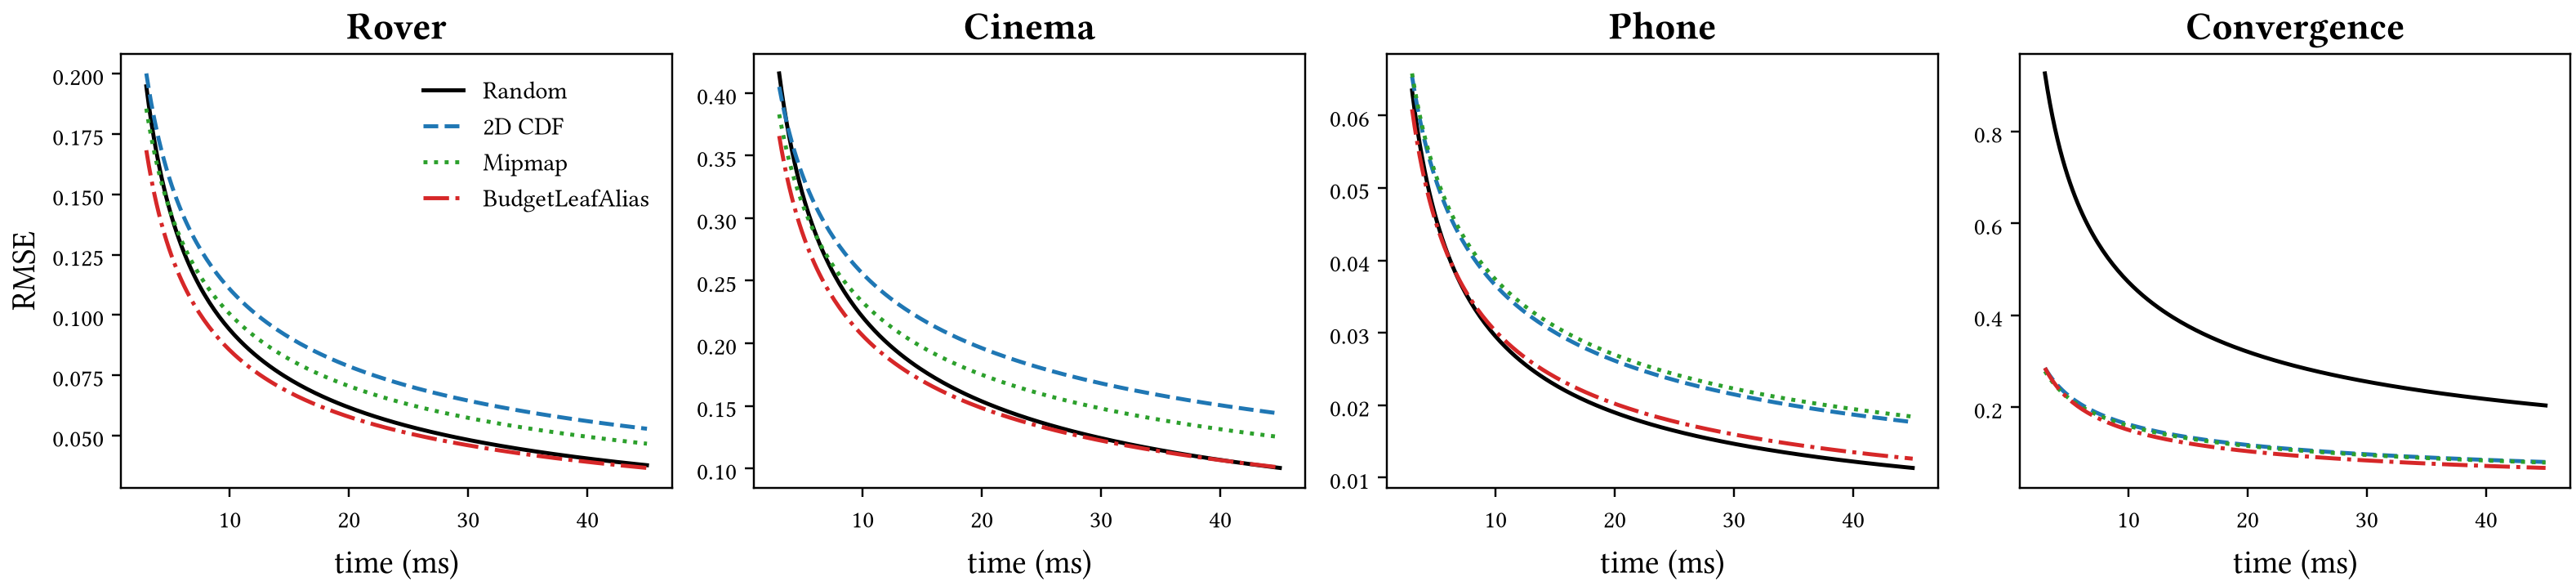
\includegraphics[width=\textwidth]{realtime_curves.png}
  \caption{Fitted RMSE-vs-time curves for Rover, Cinema, Phone, and Convergence, and all four
  techniques. BudgetLeafAlias (red) stays below both 2D CDF
  (blue) and Mipmap (green) across the entire measured range on every scene. }
  \label{fig:realtime}
\end{figure*}

\subsection{\texorpdfstring{\newt{Comparison at equal samples}}{Equal samples}}
\label{sec:equalsamples}

\newbegin
This experiment compares the techniques at the same number of samples for each scene: 4 spp and 2 light samples per vertex. We aim at measuring the variance introduced by using the LeafAlias technique. All techniques render the representative frame of each scene, 24 times with independent random numbers, and the results are compared against a converged reference (Figure~\ref{fig:equalsamples}). The three techniques that importance sample the emitter at full texel resolution (the 2D CDF, the mipmap warp and the per-pixel Alias table) reach the same error within 1\% on every scene. They sample the same distribution and differ only in how they invert it, so at equal samples, and with the independent random numbers of our renderer, they are expected to coincide. Random sampling is clearly worse: its RMSE is 1.12 and 1.21 times that of the 2D CDF on Rover and Cinema, and 1.55, 2.23 and 2.37 times on Phone, Fireplace Room and Convergence. The 2D CDF at $1/8$ resolution is up to 2.6\% behind the full-resolution techniques.

\begin{figure}[htbp!]
  \centering
  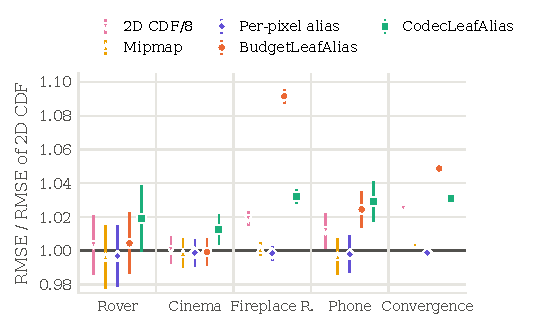
\includegraphics[width=\columnwidth]{fig_equal_samples.pdf}
  \caption{\newmat RMSE of each technique relative to the 2D CDF, with every technique using the same samples per pixel and light samples per shading point (mean of 24 renders, 95\% intervals). Random sampling, at 1.12 to 2.37, is outside the plotted range. }
  \label{fig:equalsamples}
\end{figure}

Our two techniques are slightly behind the full-resolution techniques. Relative to the 2D CDF, the RMSE of BudgetLeafAlias is $+0.4\%$ on Rover, $-0.2\%$ on Cinema, $+2.5\%$ on Phone, $+4.9\%$ on Convergence and $+9.2\%$ on Fireplace Room; that of CodecLeafAlias is $+1.2$ to $+3.3\%$ on all five scenes. The cause is the resolution of the density: both techniques choose a leaf in proportion to its mean luminance and then a point uniformly within the leaf, so the variation of luminance inside a leaf is not importance sampled. CodecLeafAlias has more and smaller leaves on such detailed content and loses less there, but its partition follows image detail rather than light, so it also spends leaves where they do not help. Figure \ref{fig:closeupsequalsamples} shows some rendering closeups for different techniques under the same number of samples.

\begin{figure}[htbp!]
  \centering
  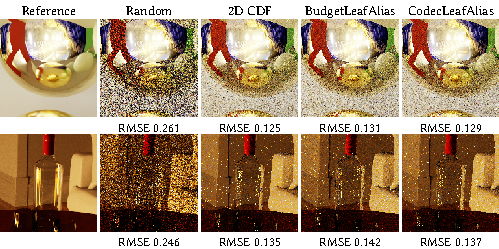
\includegraphics[width=\columnwidth]{closeup_examples.pdf}
  \caption{\newmat Examples of rendering closeups under different techniques with the same number of samples on the Convergence and Fireplace Room scenes.   }
  \label{fig:closeupsequalsamples}
\end{figure}

At equal samples, therefore, our techniques do not sample better than a texel-resolution distribution, and are not meant to: they trade a small loss of sampling quality for a much lower cost per sample and per frame.
\newend

\subsection{\texorpdfstring{\newt{Comparison at equal quality}}{Equal quality}}
\label{sec:equalquality}

\newbegin
In this experiment, we measure how long does each technique need to reach the quality that the 2D CDF delivers in real-time. 
For each scene we render the videos only with direct illumination, where the light sampler controls most of the noise. The 2D CDF uses the number of light samples that fits a 33.3\,ms frame. Every other technique is rendered with several numbers of light samples, and we find the frame time at which its video RMSE equals that of the 2D CDF. The speed-up is the frame time of the 2D CDF divided by that time.

Our two techniques reach the quality of the 2D CDF faster on all five scenes (Table~\ref{tab:equalquality}). These figures use the median frame time of each technique over several timing passes. The other techniques are not consistent: the mipmap warp is slower than the 2D CDF on Rover and does not reach its quality on Phone at the measured sample counts, and the per-pixel Alias table, which is fast on Full HD emitters, is slower than the 2D CDF on the two scenes with 4K emitters, where its memory consumption grows considerably. The time saved can be returned to the frame rate, to more bounces, or to a denoiser.

\begin{table}[htbp!]
\centering\small\newmat
\setlength{\tabcolsep}{3pt}
\caption{\newmat Speed-up of the different techniques over 2D CDF to reach the same average RMSE in the full video.}
\label{tab:equalquality}
\resizebox{\columnwidth}{!}{%
\begin{tabular}{l c c c c c}
\toprule
Technique & Rover & Cinema & Fireplace R. & Phone & Convergence \\
\midrule
2D CDF/8 & 1.17 & 1.89 & 1.29 & 1.17 & 1.17 \\
Mipmap & 0.85 & 1.45 & 1.10 & -- & 1.06 \\
Per-pixel Alias & 1.17 & 1.91 & 0.91 & 1.26 & 0.93 \\
BudgetLeafAlias & 1.31 & 2.23 & 1.19 & \textbf{1.47} & 1.27 \\
CodecLeafAlias & \textbf{1.38} & \textbf{2.31} & \textbf{1.54} & 1.23 & \textbf{1.37} \\
\bottomrule
\end{tabular}}
\end{table}

\paragraph{Emitter resolution}
The last observation suggests that the resolution of the emitter influences the advantage of our techniques. To isolate it, we render using the same emissive texture at three resolutions on the LED wall of the Rover scene: 1820$\times$1024, 3640$\times$2048 and 7280$\times$4096, obtained by area averaging from a real 8K HDR panorama of a road under broad daylight. We render frames with direct illumination, measuring time and RMSE at varying samples per pixel, and smooth the RMSE curve of each technique with a quadratic fit (Figure~\ref{fig:wall}).

\begin{figure}[htbp!]
  \centering
  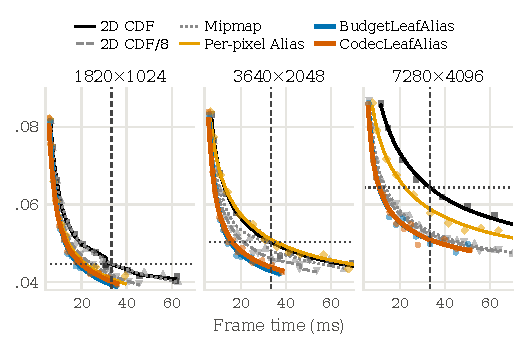
\includegraphics[width=\columnwidth]{fig_wall.pdf}
  \caption{\newmat The same image on the LED wall of the Rover scene at three resolutions: RMSE against frame time (markers: measurements; curves: fits). The vertical line is the 33.3\,ms budget and the horizontal line the RMSE of the 2D CDF at that budget. As the image grows, the curve of the 2D CDF moves to the right and ours stay almost in place.}
  \label{fig:wall}
\end{figure}

The cost of a light sample grows with resolution for the 2D CDF, and much less for our techniques. Each additional light sample per shading point adds 0.95, 1.17 and 2.93\,ms to the frame of the 2D CDF at the three resolutions, and 0.47, 0.50 and 0.73\,ms to that of BudgetLeafAlias. The 2D CDF searches a table as large as the image, with one dependent memory read per search step, and at 8K that table is sixteen times larger than at Full HD; ours read a table of about 75\,KB at any resolution, and the image only once the texel has been chosen. In a 33.3\,ms frame the 2D CDF therefore fits 34, 25 and 10 light samples, while BudgetLeafAlias fits 60, 58 and 40.

As a result, the speed-up at equal quality grows at 8K: both techniques reach the quality of the 2D CDF up to 3$\times$ faster. Read at equal time, the RMSE of BudgetLeafAlias is 12\%, 15\% and 21\% lower than the 2D CDF's. The per-pixel Alias table follows the 2D CDF, since its table also grows with the image and its memory access patterns are more incoherent. The two baselines that keep small or hierarchical structures, the 2D CDF at one eighth of the resolution and the mipmap warp, scale better and reach 2.67 and 2.44 times at 8K; they remain behind our techniques at every resolution. 
\newend

\subsection{\texorpdfstring{\newt{Sampling cost on the GPU}}{Sampling cost on the GPU}}
\label{sec:cost}

\newbegin
We relate the cost of drawing a light sample to the cache levels of the GPU with two benchmarks (Figure~\ref{fig:cache}). In the left figure, a pointer chase reads memory in a chain of dependent random accesses as the working set grows from 4\,KB to 512\,MB. It shows a sharp limit: dependent reads cost about 3\,ps (in aggregate over the whole GPU) while the data fits in the first-level cache, but three times as much once the working set exceeds 128--192\,KB, and tens of times more beyond the second-level cache (64\,MB on our GPU). 

\begin{figure}[htbp!]
  \centering
  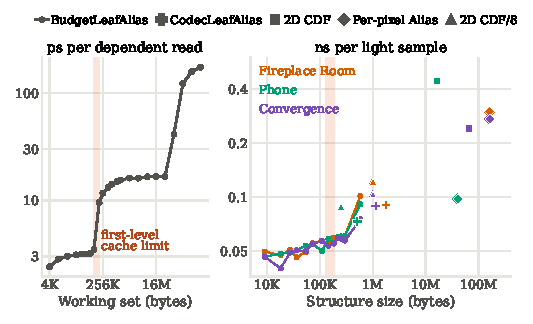
\includegraphics[width=\columnwidth]{fig_gpu_cost2.pdf}
  \caption{\newmat Left: latency of dependent random reads against the size of the data being read, on the GPU (pointer chase, aggregate over the whole GPU). Right: measured cost of one light sample against the size of the sampling structure: BudgetLeafAlias from 64 to 32000 leaves (lines), CodecLeafAlias, and the 2D CDF, per-pixel Alias and 2D CDF/8 (markers), in three scenes. }
  \label{fig:cache}
\end{figure}

In the second figure, we measure the time it takes to draw a sample and read the emissive texture, with varying $B$ values and the other techniques.
The emissive texture read is generally fast because most of the samples point to the same bright sections of the image, hence hitting cache more frequently. These results show the same behavior as the left figure. A sample of the 2D CDF costs between 0.23\,ns and 0.46\,ns, as throughput of the whole GPU, and we give the cost of the other techniques relative to it. BudgetLeafAlias at $B=4000$ is 4 to 8 times cheaper, and its cost hardly changes with the scene; CodecLeafAlias, whose table is larger, costs 1.3 to 1.6 times as much as BudgetLeafAlias. 

The per-pixel Alias table costs a quarter of the 2D CDF on the Full HD emitter of Phone, but 1.2 times as much on the 4K emitter of Convergence. This is explained by the fact that its structure, despite being $O(1)$ to sample, performs two dependent reads per sample at addresses spread uniformly over the whole structure, so almost every read misses the first-level cache; at 4K the structure exceeds the second-level cache as well, and the cost per sample more than doubles.  The 2D CDF performs 24 dependent reads per sample in the worse case, but most of them are cache hits: the marginal CDF is a few kilobytes, and the conditional searches concentrate on the few bright rows.
\newend

\subsection{\texorpdfstring{\newt{Leaf budget}}{Leaf budget}}
\label{sec:leafbudget}

\newbegin
In the next experiment, we sweep the leaf budget $B$ of BudgetLeafAlias from 16 to 16000 leaves in the five scenes at varying number of light samples per pixel. Figure~\ref{fig:leafbudget} shows the error of each budget relative to $B=4000$ at equal samples, so that only the quality of the leaf density is compared.

\begin{figure*}[htbp!]
  \centering
  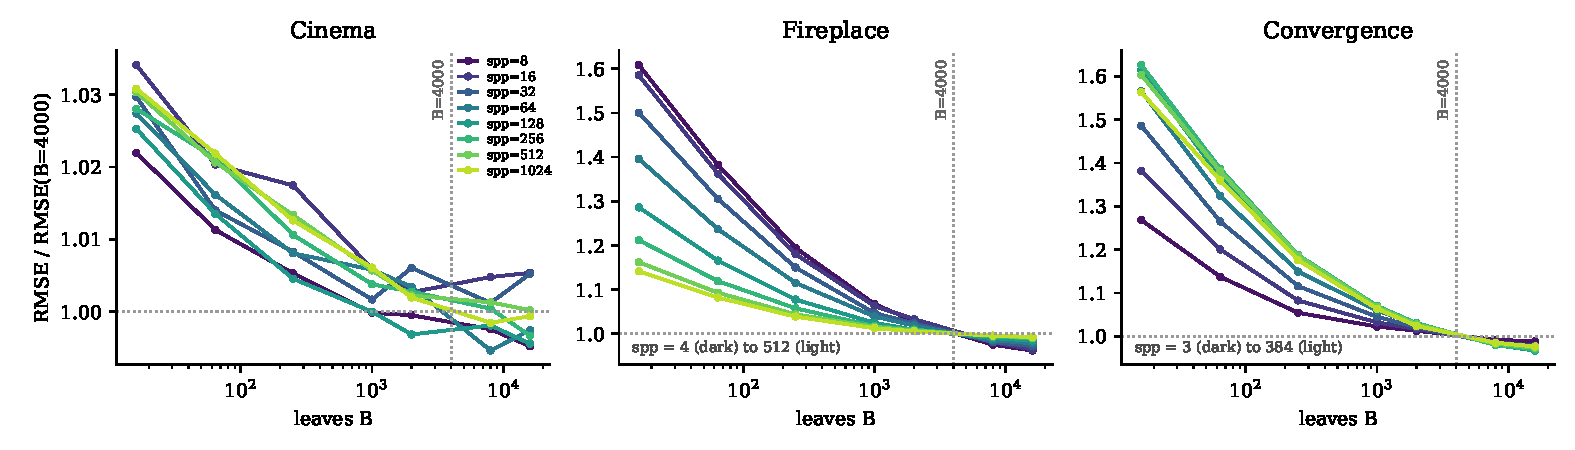
\includegraphics[width=0.92\textwidth]{fig_leaf_budget.pdf}
  \caption{\newmat RMSE against the converged reference, divided by the RMSE of $B=4000$ at the same number of light samples per pixel (spp), as a function of the leaf budget $B$. Values above 1 mean more error than $B=4000$.}
  \label{fig:leafbudget}
\end{figure*}

Two behaviors appear, depending on how the light is distributed over the emitter. In Cinema, light is spread over most of the screen, and a coarse partition already results in one figure error percentages. Rover and Phone behave in a similar way (not shown). In Fireplace Room and Convergence, most of the energy sits in small regions that the partition must resolve, and the error falls steeply with $B$ before levelling off. In Convergence, 250 leaves give up to 1.20 times the error of $B=4000$,  and 1000 leaves up to 1.07 times, while doubling or quadrupling the budget beyond 4000 improves the error by only 1--3\% at every sample count. 

On the cost side, as we saw in the previous section, the structure grows linearly with $B$, and the performance penalty is minimized as long as the sampler resides in L1 cache. $B=4000$ therefore sits at the knee of both curves: it captures nearly all the quality available from the partition, and at 75\,KB it uses most of the cache without exceeding it. $B$ acts as a memory and quality knob, and devices with smaller caches or less memory can use a smaller budget at the quality cost shown in Figure~\ref{fig:leafbudget}. All these measurements are on one GPU; the \supp{ablation\_leaf\_number} contains the complete tables and the  \supp{GPU\_tests} contain results for a mobile GPU device, showing similar patterns when using less cores and memory.
\newend



\subsection{\texorpdfstring{\newt{Frequency of frame partitions}}{Frequency of frame partitions}}
\label{sec:static}

\newbegin
As an alternative to rebuilding the partition every frame, we analyze the error generated by building the tree and leaf weights with less frequency. We compare under equal number of samples: (i)~one tree and one set of weights computed from the average of all frames, with 5\% of the probability spread uniformly to keep the estimator unbiased; (ii)~the same average tree with the weight of each leaf recomputed at each frame; (iii)~a tree rebuilt every 30 frames, with per-frame weights; and (iv)~BudgetLeafAlias. Table~\ref{tab:average-tree} reports the quality of each over the full videos.

\begin{table}[t]
\centering\small\newmat
\setlength{\tabcolsep}{4pt}
\caption{\newmat Quality for static, partially updated and per-frame trees, with 4000 leaves and equal samples per scene (samples per pixel $\times$ light samples per shading point in parentheses). The keyframe tree is rebuilt every 30 frames. The last row of each scene is the ratio of RMSE to BudgetLeafAlias, calculated before rounding. \aspnote{target values; measured now, RMSE ratio: average tree with average weights 1.02--1.40, average tree with per-frame weights 1.002--1.035, keyframe tree 1.00--1.04}}
\label{tab:average-tree}
\resizebox{\columnwidth}{!}{%
\begin{tabular}{l l c c c c}
\toprule
 &  & \shortstack{Avg. tree\\and weights} & \shortstack{Avg. tree,\\per-frame weights} & \shortstack{Keyframe tree,\\per-frame weights} & \textbf{\shortstack{Every frame\\(BudgetLeafAlias)}} \\
\midrule
\textit{Rover} & RMSE $\downarrow$ & 0.0883 & 0.0845 & 0.0842 & 0.0780 \\
(4$\times$2) & PSNR $\uparrow$ & 21.09 & 21.48 & 21.50 & 22.17 \\
 & VMAF $\uparrow$ & 71.0 & 72.0 & 72.1 & 73.4 \\
 & RMSE ratio $\downarrow$ & 1.132 & 1.083 & 1.080 & 1 \\
\midrule
\textit{Cinema} & RMSE $\downarrow$ & 0.0823 & 0.0809 & 0.0825 & 0.0748 \\
(4$\times$1) & PSNR $\uparrow$ & 22.65 & 22.80 & 22.63 & 23.48 \\
 & VMAF $\uparrow$ & 72.8 & 73.3 & 72.9 & 74.6 \\
 & RMSE ratio $\downarrow$ & 1.100 & 1.082 & 1.103 & 1 \\
\midrule
\textit{Fireplace Room} & RMSE $\downarrow$ & 0.1077 & 0.0990 & 0.1008 & 0.0905 \\
(4$\times$1) & PSNR $\uparrow$ & 19.36 & 20.09 & 19.93 & 20.87 \\
 & VMAF $\uparrow$ & 53.8 & 57.4 & 56.9 & 59.2 \\
 & RMSE ratio $\downarrow$ & 1.190 & 1.094 & 1.114 & 1 \\
\midrule
\textit{Phone} & RMSE $\downarrow$ & 0.0353 & 0.0295 & 0.0298 & 0.0272 \\
(4$\times$1) & PSNR $\uparrow$ & 29.38 & 30.93 & 30.83 & 31.63 \\
 & VMAF $\uparrow$ & 79.5 & 80.7 & 80.4 & 81.8 \\
 & RMSE ratio $\downarrow$ & 1.296 & 1.084 & 1.097 & 1 \\
\midrule
\textit{Convergence} & RMSE $\downarrow$ & 0.1866 & 0.1414 & 0.1418 & 0.1268 \\
(4$\times$4) & PSNR $\uparrow$ & 14.70 & 17.11 & 17.09 & 18.06 \\
 & VMAF $\uparrow$ & 50.3 & 60.4 & 60.2 & 62.4 \\
 & RMSE ratio $\downarrow$ & 1.472 & 1.115 & 1.118 & 1 \\
\bottomrule
\end{tabular}}
\end{table}


Rebuilding the tree and its weights every frame gives the lowest error in every scene. A fully static structure raises the RMSE by 10\% on Cinema, 13\% on Rover, 19\% on Fireplace Room, 30\% on Phone and 47\% on Convergence, where VMAF falls by 12 points: fixed weights cannot adapt to changes of the light distribution, and the uniform share spends samples on regions that are dark in a given frame. Recomputing the weights of the average tree every frame recovers most of that loss, but the fixed topology remains 8--12\% behind the per-frame tree, and a tree rebuilt once per second is 8--12\% behind as well.

These results suggest that rebuilding the partition every frame is needed, especially for dynamic content with moving bright spots like the Convergence environment map. The average tree, in addition, requires the whole video in advance, which live and streamed content does not provide, and the per-frame rebuild needs no keyframe interval and adapts at once to cuts, fades and sudden changes of light, where a stale tree is at its worst.

\paragraph{Temporal stability.} Since the partition changes from frame to frame (3--13\% of the $8{\times}8$ cells change leaf size per frame), we measured whether this introduces flicker. Appendix~\ref{app:temporal} gives the metrics and the measurements that show that the leaf density changes \emph{less} between consecutive frames than the exact per-texel density in four of the five scenes, and the low-frequency temporal error of the rendered video, the part perceived as flicker, is equal to or lower than that of the 2D CDF for BudgetLeafAlias in every scene, before and after denoising. 
\newend

\subsection{\texorpdfstring{\newt{Codec partitions}}{Codec partitions}}
\label{sec:codecstudy}

\newbegin

This section analyzes the effect of using the codec partition in CodecLeafAlias as opposed to constructing it based on a leaf number budget. 
Figure~\ref{fig:partitions} shows two examples of partitions, where the codec version is more refined in high-variance parts of the images.
To compare the partitions independently of the renderer, we compute the light-sampling variance factor of the density, $V = \sum_i f_i^2/p_i - 1$, where $f$ is the normalized luminance of the frame and $p$ the sampling density per texel; $V$ is the relative variance of a one-sample estimate of the emitter's power, and is zero for a density proportional to the frame. $V$ isolates the light-sampling part of the error and so changes far more than the rendered error.

\begin{figure}[htbp!]
  \centering
  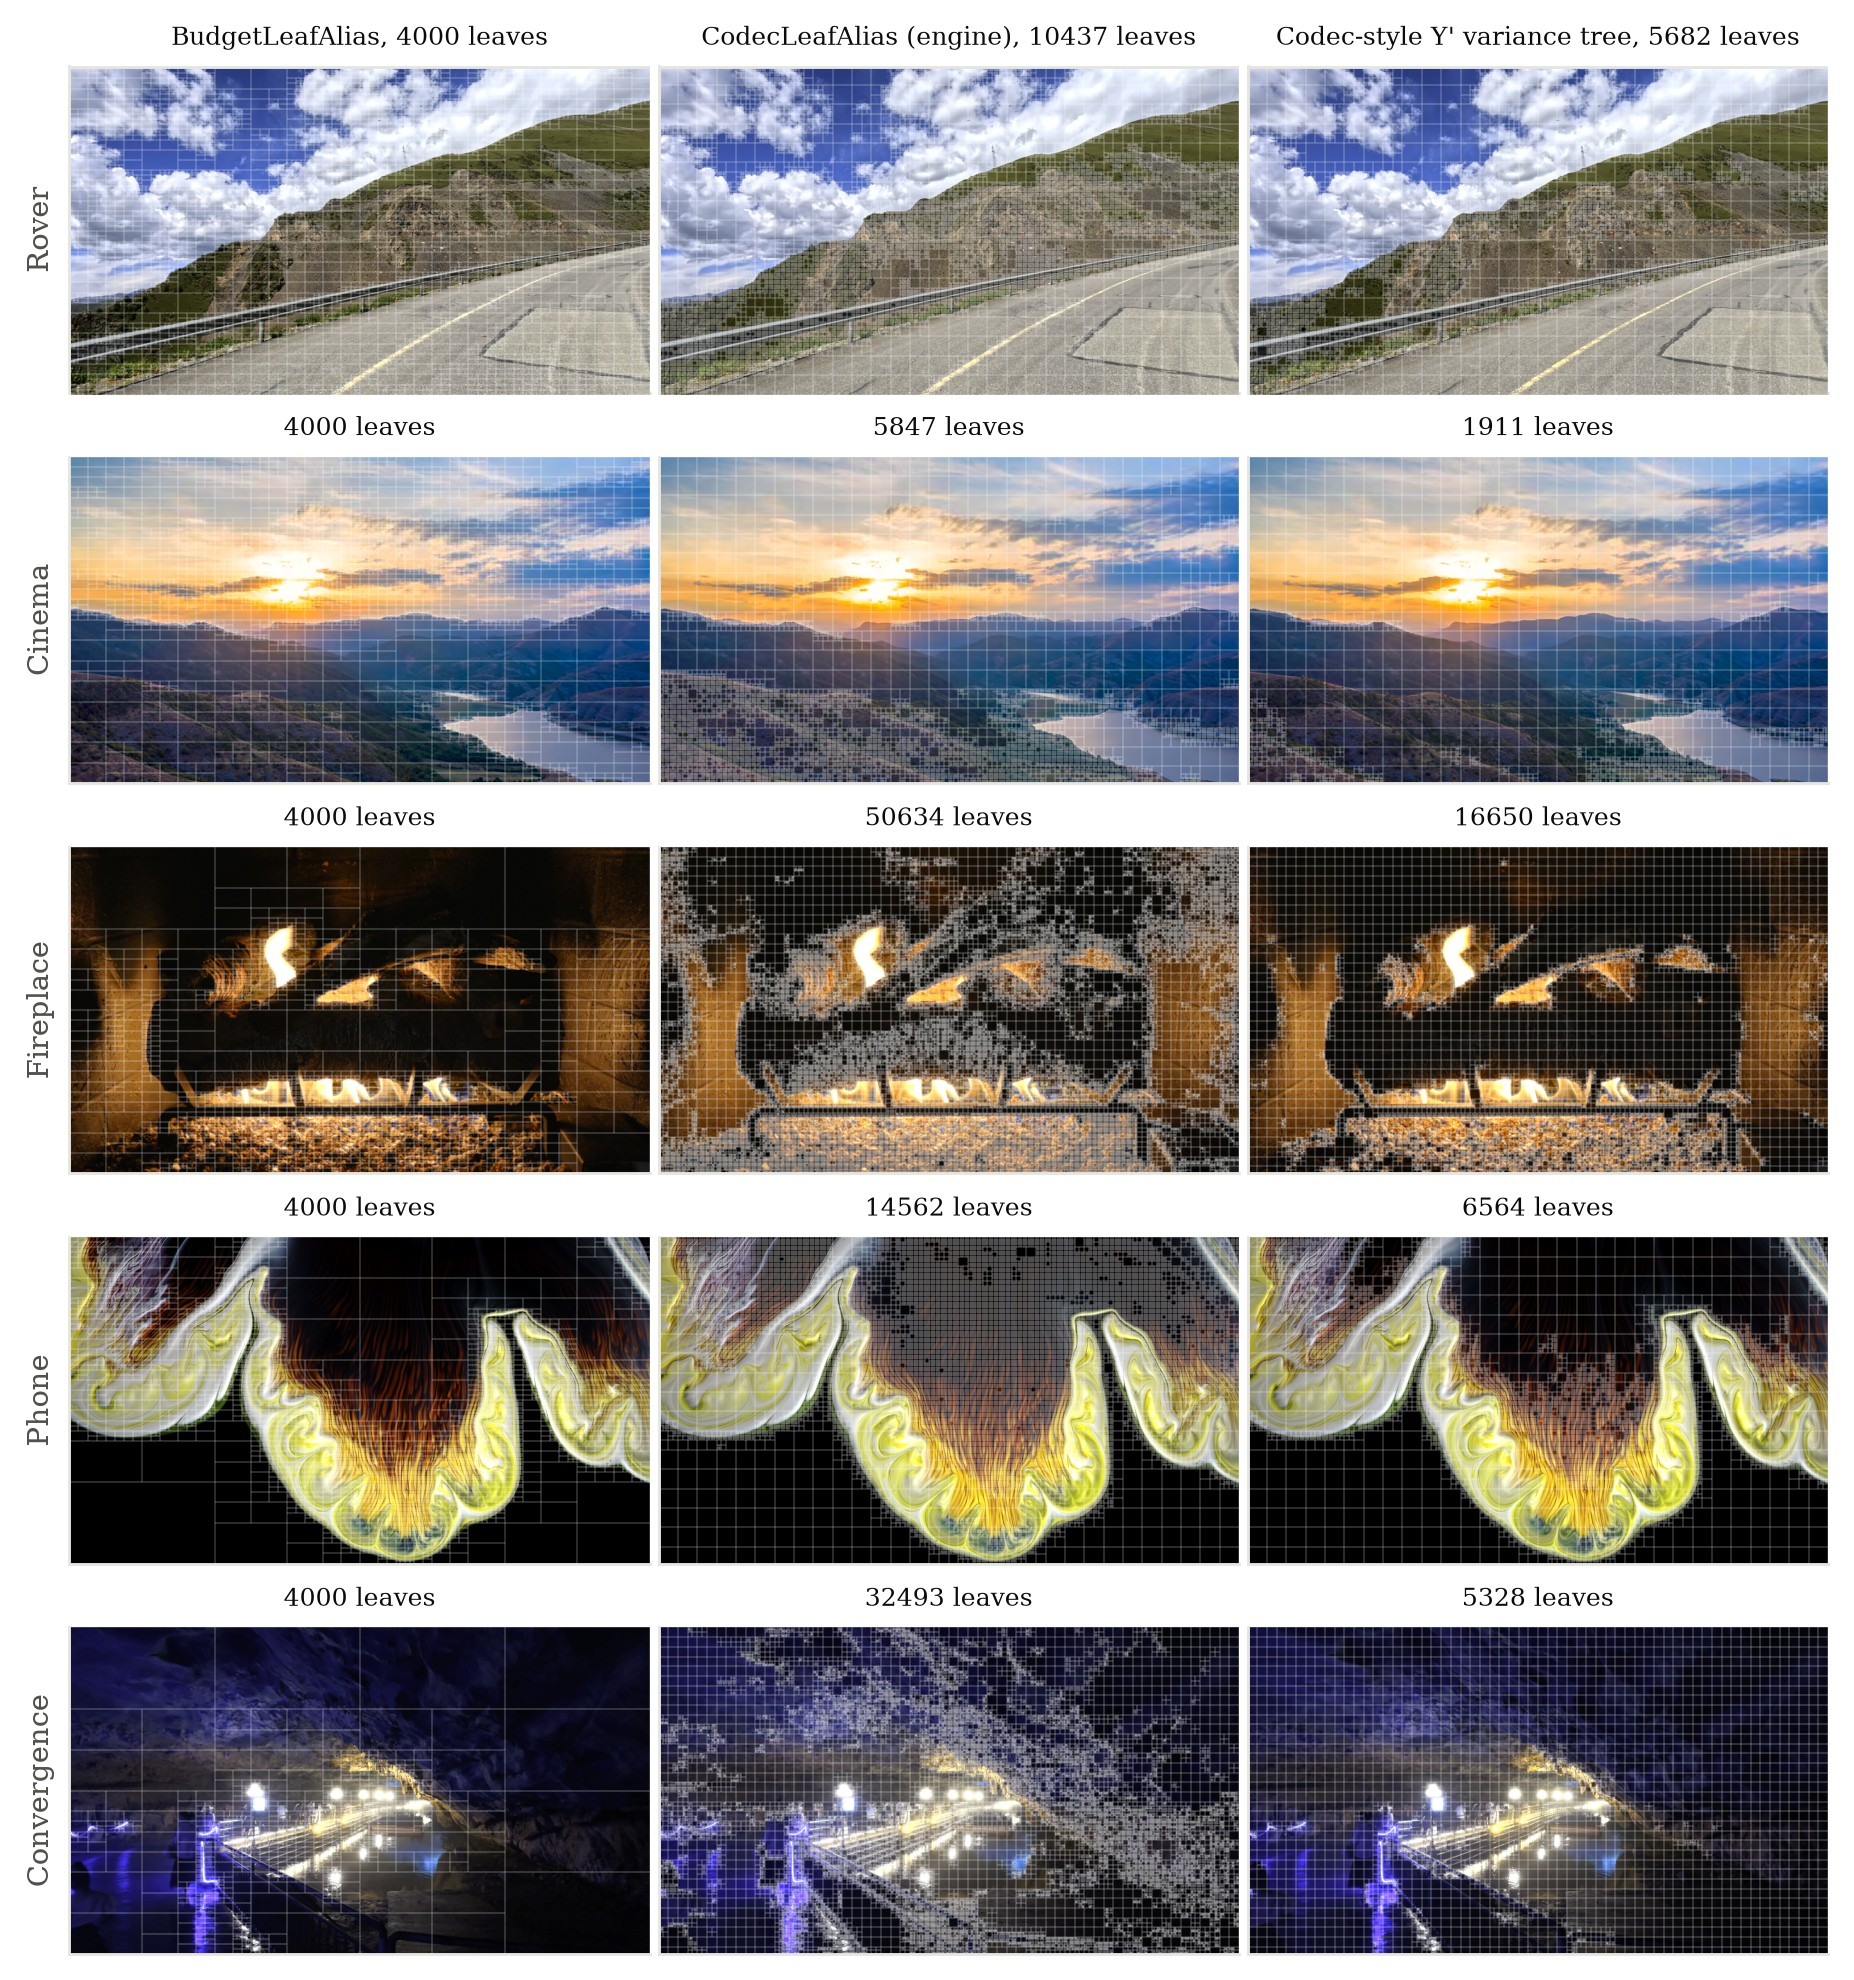
\includegraphics[width=\columnwidth]{fig_partitions.jpg}
  \caption{\newmat Leaf partitions of one frame of Rover and Phone. .}
  \label{fig:partitions}
\end{figure}

Figure~\ref{fig:variance} shows variance against leaf count for BudgetLeafAlias at varying number of leaves, and CodecLeafAlias. 
The plots show that codec leaves are placed less usefully for light sampling in every scene the codec partition lies above the budget curve, and BudgetLeafAlias reaches the same variance with 23--54\% of its leaves (94\% in Phone). A codec partition helps when it has considerably more leaves than the budget: in Fireplace Room it has about 47000 leaves, 12 times the budget, and reaches 0.26 of its variance; in Convergence about 27000 and 0.48. Rendered at equal samples, CodecLeafAlias is accordingly 5.3\% better than BudgetLeafAlias in Fireplace Room and 1.7\% better in Convergence (Figure~\ref{fig:equalsamples}), and it has the best full-video result on those two scenes (Table~\ref{tab:main}). 

\begin{figure}[htbp!]
  \centering
  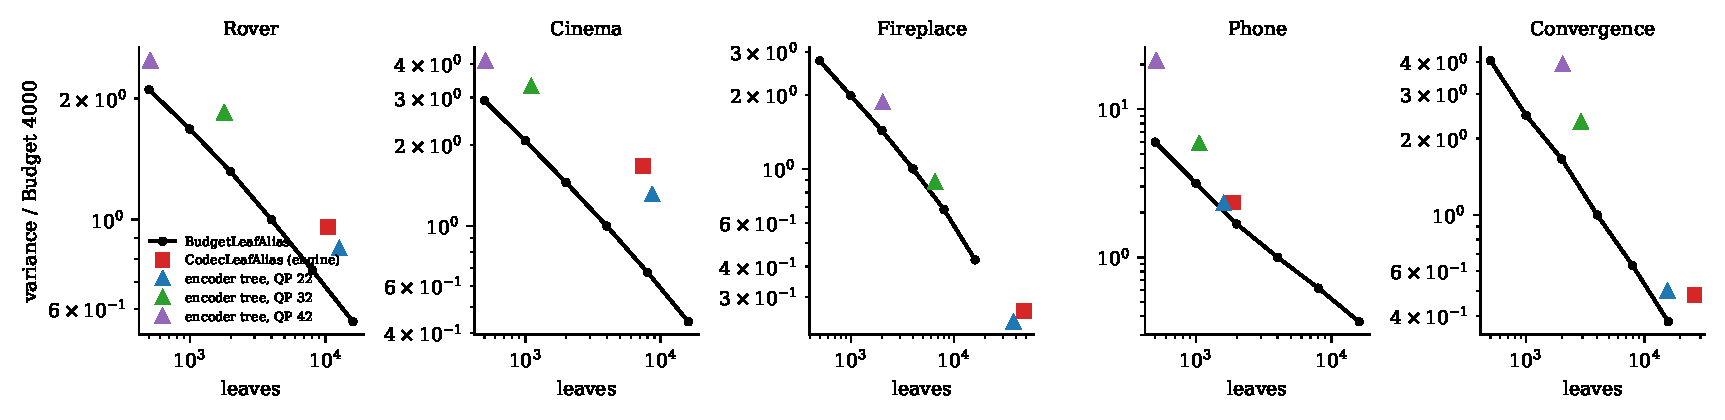
\includegraphics[width=\columnwidth]{fig_variance_vs_leaves.pdf}
  \caption{\newmat Light-sampling variance against leaf count, relative to BudgetLeafAlias with 4000 leaves (median over frames). Each line is BudgetLeafAlias from 500 to 16000 leaves in one scene, and the square of the same color is the CodecLeafAlias partition of that scene. }
  \label{fig:variance}
\end{figure}

A codec partition fails in two situations. On dark or low-contrast content the leaves go to dark detail: the Cinema partition has 7400 leaves and still 1.67 times the variance of 4000 budget leaves. And the leaf count swings with the content, by 40 times within the Phone video (528 to 20133), and with it the memory (0.2 to 2.2\,MB per frame) and the sampling cost, against a fixed 75\,KB. In summary, CodecLeafAlias is preferable when a decoded stream is at hand, the light is concentrated or the content bright and detailed, and a variable memory footprint is acceptable. BudgetLeafAlias is preferable when memory or cache size must be bounded, on dark or fading content, whenever predictable cost matters, and for emissive textures that are not decoded from a stream at all (rendered, procedural or uncompressed). The two can be combined by merging a codec partition down to a budget with the same $\mathrm{Var}\cdot A$ rule. 

\paragraph{Quantization and bitrate.}
As discussed in Section~\ref{sec:codec}, compression does not introduce bias to the estimate, so the question is how much variance it adds. We encoded the five videos in 10-bit PQ with libvpx-vp9 (CRF 12, 32, 48, 63), x265 (CRF 18, 28, 40) and SVT-AV1 (CRF 25, 40, 55), from 74 down to 0.6\,Mb/s (decoded PSNR from 51 to 32\,dB), took the leaf weights from the decoded planes as described in Section~\ref{sec:codec}, and rendered one inter-coded frame per scene at equal samples (32 captures) against the same partition with exact leaf weights.

Every ratio lies between 0.995 and 1.029 (Figure~\ref{fig:rate}), the largest PSNR loss is 0.23\,dB, and the ratios do not grow as the bitrate falls: compression error is spread over each block, while a leaf weight is the mean over the whole leaf, so most of it averages out. Taking the partition from the decoded frame instead of the source gives 0.996--1.019. Quantizing the block means directly isolates the effect of the DC quantizer: up to a step of 64 of the 1023 code values the error grows by about 3\% at most, for both partitions, and only a step of 256, a quarter of the range, reaches 4--13\%. Using the luma mean alone instead of the three planes changes the error by at most 1.5\%. 

\begin{figure}[htbp!]
  \centering
  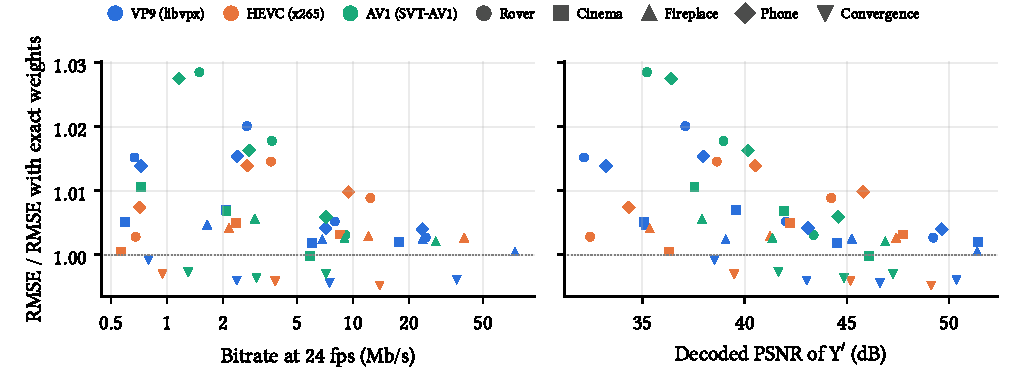
\includegraphics[width=\columnwidth]{fig_rate_sensitivity.pdf}
  \caption{\newmat RMSE of the rendered frame with leaf weights taken from lossy encodes, relative to exact leaf weights, against bitrate (left) and decoded PSNR (right), for three codecs and five scenes. All 50 points lie between 0.995 and 1.029, with no trend toward low bitrates.}
  \label{fig:rate}
\end{figure}

\paragraph{Other codecs and encoder settings.}
CodecLeafAlias needs two things from a codec: a block partition that follows image content, and the mean of each block. Every block-based codec provides the second; the first depends on the frame type. A standard configuration chooses blocks by rate-distortion (RD) search. In an intra-coded frame this splits where the image is detailed, which is what the sampler needs. In a predicted frame the search runs on the residual left after motion compensation, so its blocks follow prediction error rather than content: where motion is predicted well, a detailed region can be coded as one large block (Figure~\ref{fig:trees}).

\begin{figure}[htbp!]
  \centering
  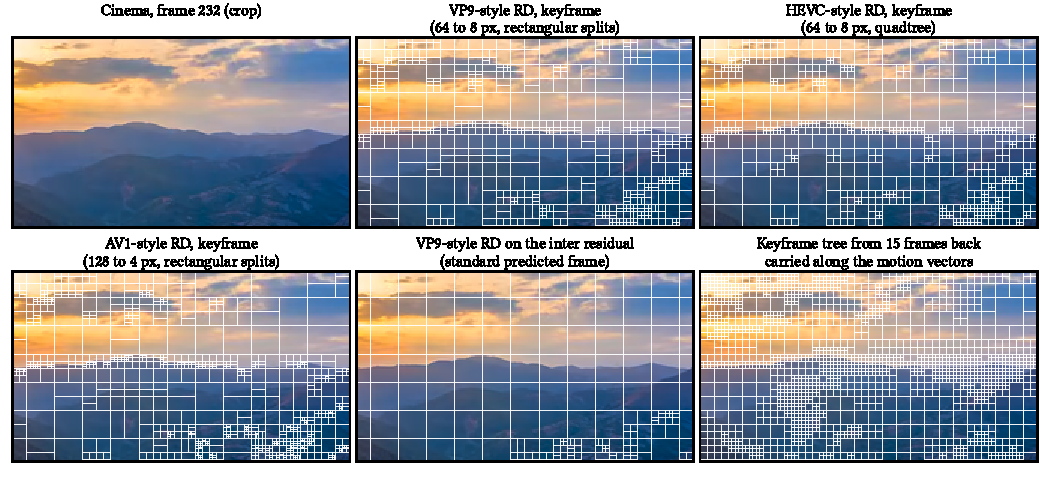
\includegraphics[width=\columnwidth]{fig_codec_trees.pdf}
  \caption{\newmat Partitions of a Cinema frame at quantizer 64 of 1023. Keyframe RD trees of the three codec families follow content. The RD tree of a predicted frame (bottom middle) follows prediction error instead and leaves most of the details in large blocks. The keyframe tree carried along the motion vectors (bottom right) follows content again.}
  \label{fig:trees}
\end{figure}

We reproduced the partition search of the three codec families on our frames, with their block sizes and split modes (VP9 and HEVC from 64 to 8 pixels, AV1 from 128 to 4), at quantizers 16, 64 and 256 of 1023, and rendered each partition with exact leaf means at equal samples. Used directly, the RD tree of a predicted frame costs up to 12\% for VP9 and HEVC and 22\% for AV1 at quantizer 64, relative to the CodecLeafAlias partition. Reusing the last keyframe's tree without moving it is better but drifts as the content moves (up to 6\%). Carrying the keyframe tree along the motion vectors of the stream, the strategy proposed in Section~\ref{sec:codec}, solves both: it stays within 2.5--4.2\% of the CodecLeafAlias partition at quantizers 16 and 64 for all three codec families, and within 5.4--6.6\% at quantizer 256, which is comparable to a partition built without any codec data. The three families behave alike for every partition source, and with weights from real encodes their worst ratios are 1.020 (VP9), 1.015 (HEVC) and 1.029 (AV1). The method is therefore tied neither to VP9 nor to its variance partitioning mode. 
\newend

\subsection{Denoised Results}
\label{sec:denoise}
Real-time renders are frequently paired with a neural denoiser in production. We pass each
technique's calibrated real-time render through the same OptiX denoiser~\cite{nvidia2021optixdenoiser} and re-measure
RMSE against the reference. Table~\ref{tab:denoise} shows that on every scene tested,
starting from our lower-noise image lets the denoiser reach a lower final RMSE than starting
from Random or 2D CDF.

\begin{table}[htbp!]
\centering
\small
\caption{RMSE before and after denoising. On every scene tested, whichever of our two techniques wins that scene keeps the lowest denoised RMSE too. }
\label{tab:denoise}
\begin{tabular}{ll cc}
\toprule
Scene & Technique & Noisy RMSE & Denoised RMSE \\
\midrule
\multirow{3}{*}{Rover}
 & Random & 0.0468 & 0.0381 \\
 & 2D CDF & 0.0779 & 0.0424 \\
 & {BudgetLeafAlias} & \textbf{0.0367} & \textbf{0.0375} \\
\midrule
\multirow{3}{*}{Cinema}
 & Random & 0.1109 & 0.0111 \\
 & 2D CDF & 0.1218 & 0.0110 \\
 & {CodecLeafAlias} & \textbf{0.0933} & \textbf{0.0106} \\
\midrule
\multirow{3}{*}{Fireplace Room}
 & Random & 0.5516 & 0.0312 \\
 & 2D CDF & 0.2295 & 0.0233 \\
 & {CodecLeafAlias} & \textbf{0.2087} & \textbf{0.0225} \\
\midrule
\multirow{3}{*}{Convergence}
 & Random & 0.3296 & 0.0148 \\
 & 2D CDF & 0.1428 & 0.0041 \\
 & {CodecLeafAlias} & \textbf{0.0870} & \textbf{0.0034} \\
\bottomrule
\end{tabular}
\end{table}


Convergence benefits the most: denoising cuts RMSE by over $95\,\%$ for every technique, and
CodecLeafAlias still finishes with the lowest denoised RMSE of the three ($0.0034$,
against $0.0041$ for 2D CDF), a direct result of feeding the denoiser a cleaner starting
image. Figure~\ref{fig:denoisedflip} additionally shows
denoised closeups and their \FLIP\  error maps for Convergence and Fireplace Room. 2D CDF's denoised output keeps a visibly brighter (higher-error) \FLIP\ map.

\new{The differences between techniques are nevertheless much smaller after denoising than before it, for two reasons. First, the denoiser removes mostly the high-frequency, per-pixel part of the error, which is precisely where light samplers differ; what remains is dominated by low-frequency residue that depends little on the number of light samples. Second, as discussed in Section~\ref{sec:equalquality}, light sampling is only one term of the error of a frame, so the room for any emission sampler is bounded before the denoiser acts. For a denoised pipeline the practical reading is the one of Section~\ref{sec:equalquality}: similar final quality is obtained from a sampler that costs less time and memory.}

Figure~\ref{fig:teaser} shows full-frame comparisons and closeups for Rover and Cinema, where
BudgetLeafAlias and CodecLeafAlias respectively remove most of the speckled noise still
visible in Random and 2D CDF's closeups. Figure~\ref{fig:figuresonly} shows
the same treatment for the remaining three scenes against a converged reference, with two matched closeups per scene; each panel also shows, in its top-left
corner, the actual HDR emissive texture that lit that scene. CodecLeafAlias visibly reduces
noise relative to both baselines.

\begin{figure*}[htbp!]
  \centering
  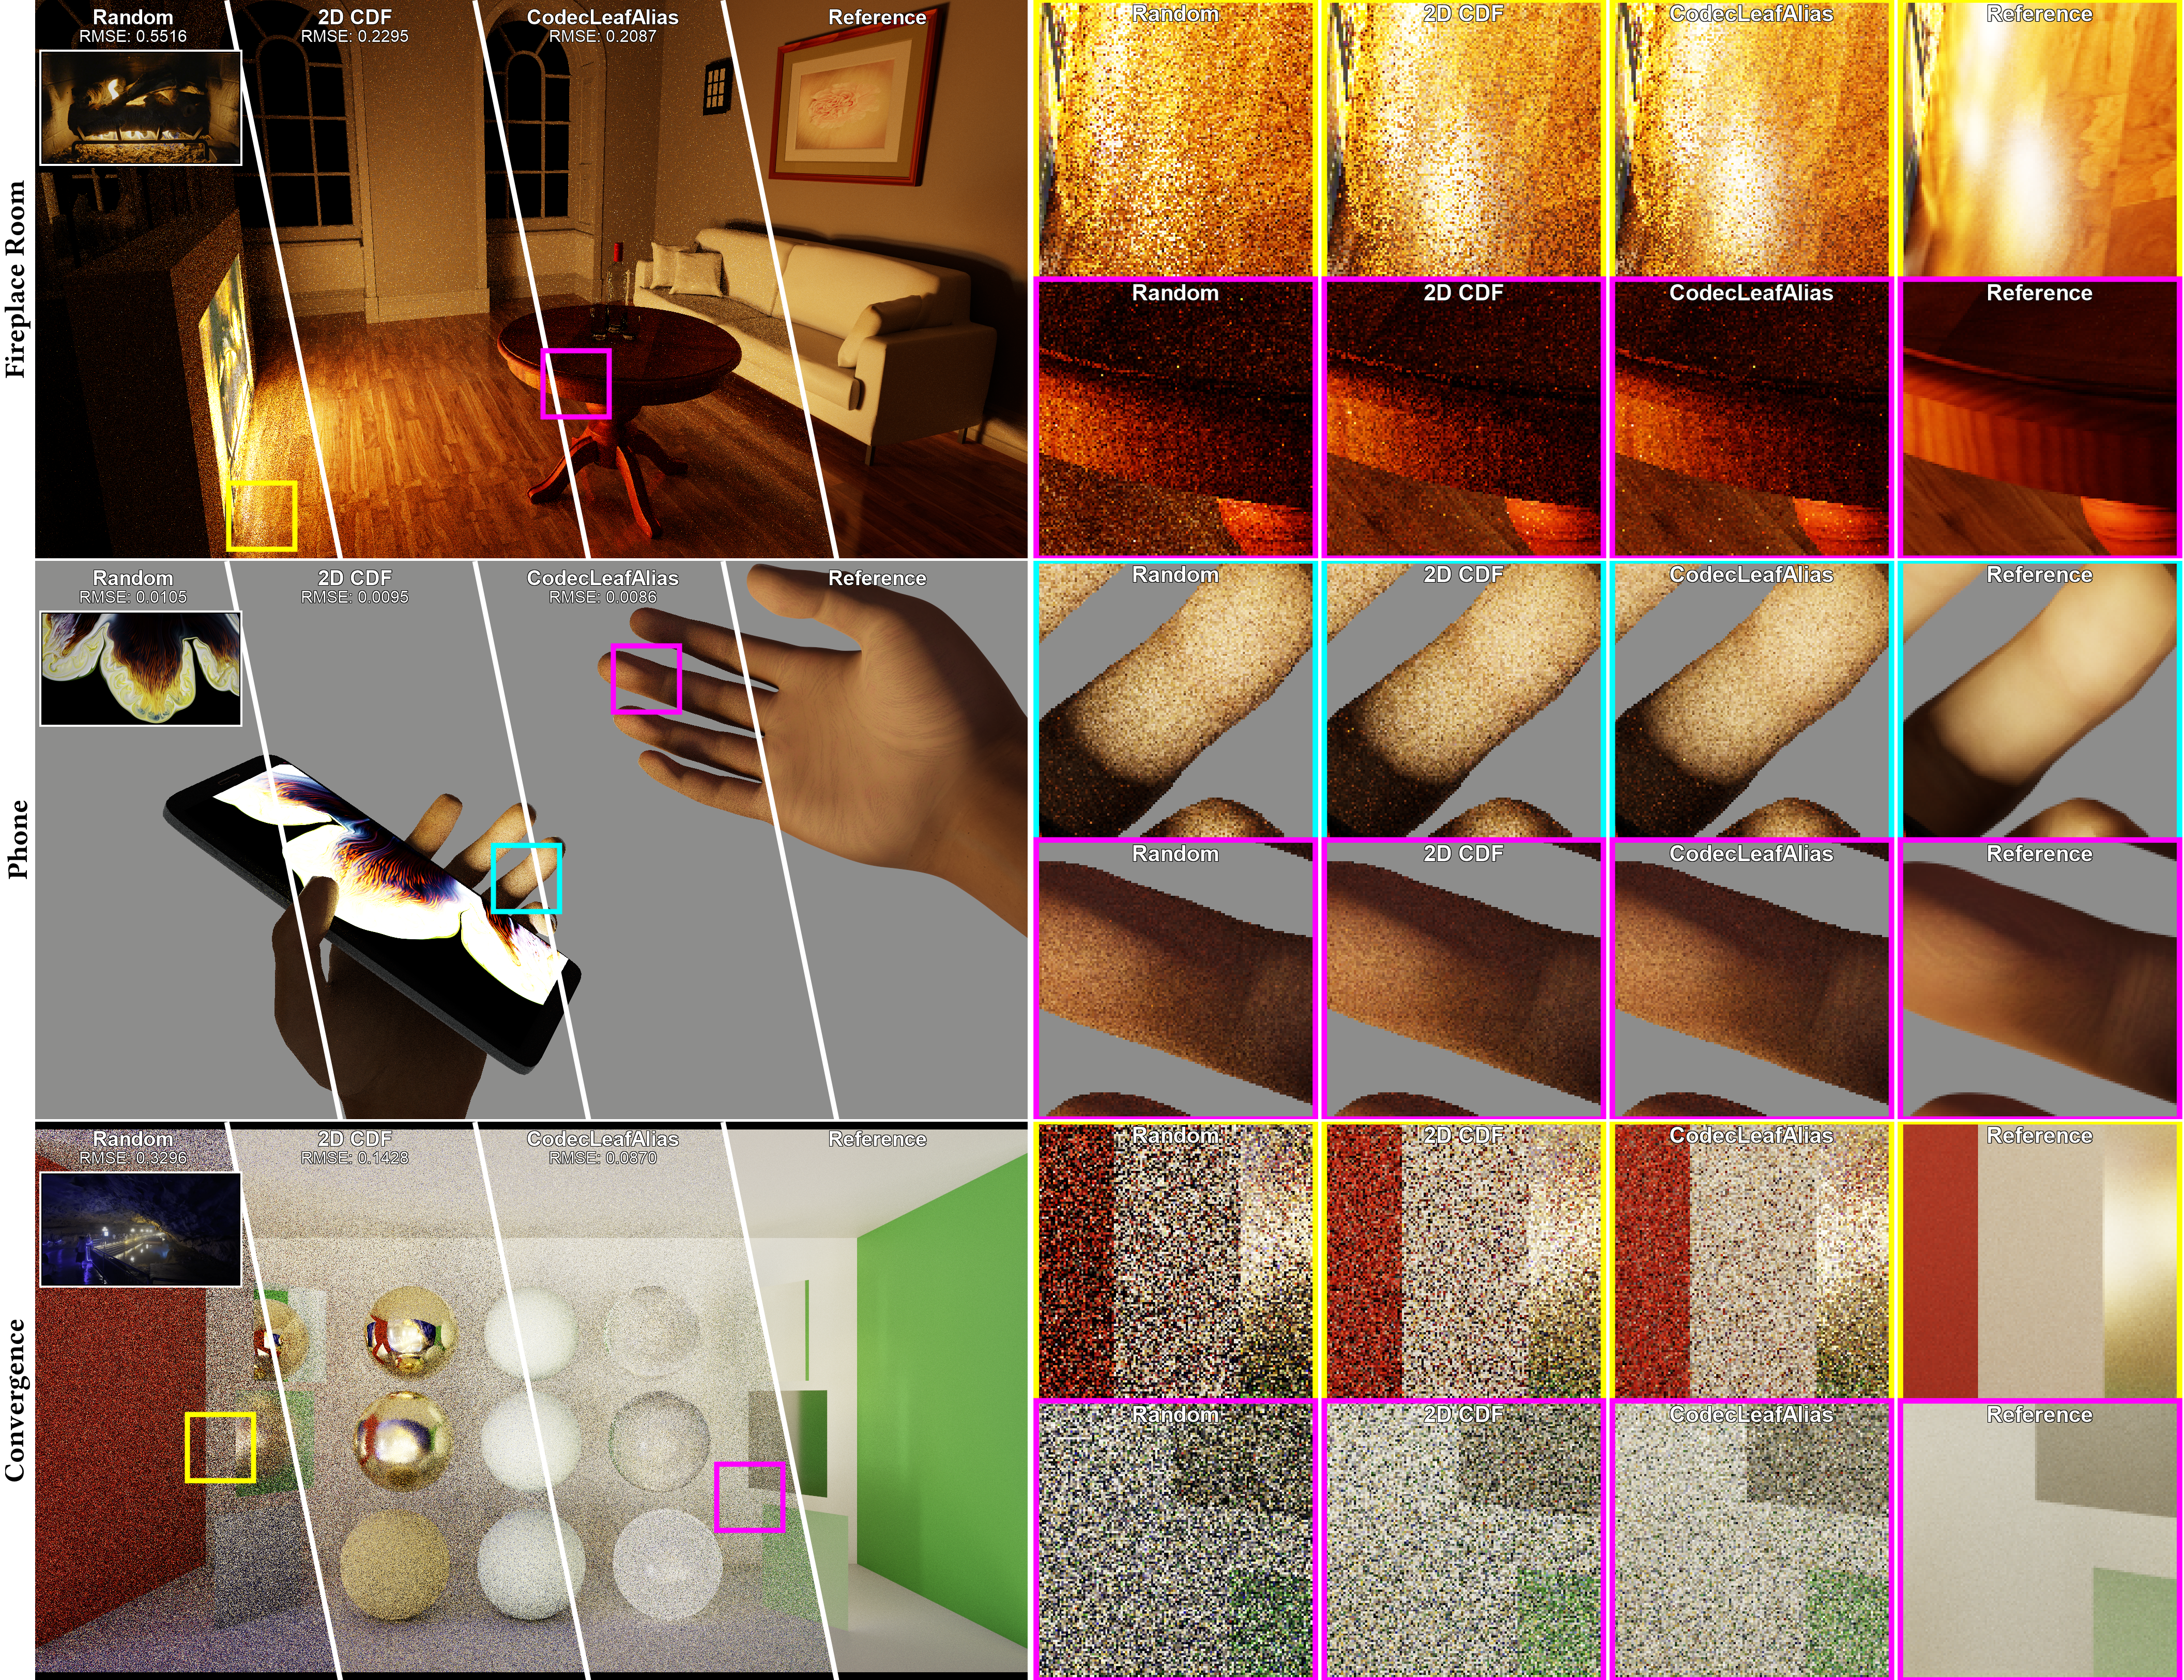
\includegraphics[width=\textwidth]{figures_only_restir_v9.png}
  \caption{Fireplace Room, Phone, and Convergence: full-frame diagonal comparisons
  (Random / 2D CDF / CodecLeafAlias / Reference) with real measured RMSE per technique, two
  large matched closeups per scene, and each scene's emissive HDR texture (top-left inset). }
  \label{fig:figuresonly}
\end{figure*}

\begin{figure*}[htbp!]
  \centering
  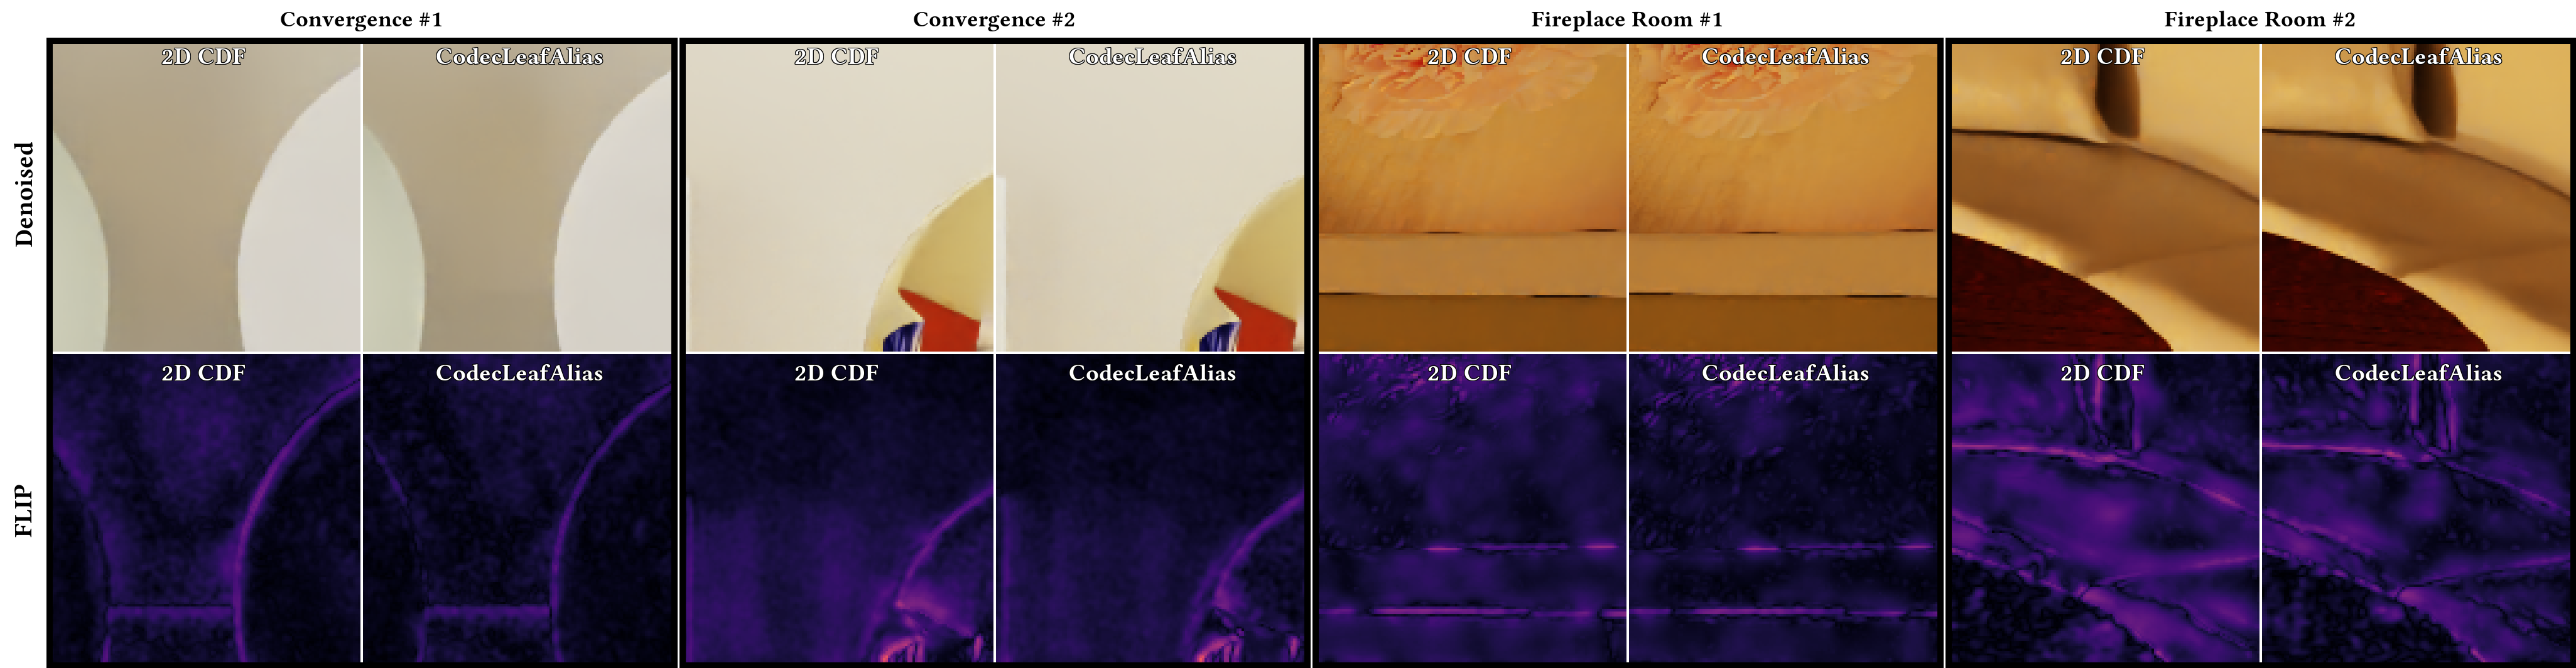
\includegraphics[width=\textwidth]{denoised_flip_grid.png}
  \caption{Denoised closeups and FLIP error maps when compared to the reference, for 2D CDF
  and CodecLeafAlias, at the two regions per scene with the largest denoised FLIP gap, for
  Convergence and Fireplace Room.}
  \label{fig:denoisedflip}
\end{figure*}

\subsection{\texorpdfstring{\newt{Discussion and limitations}}{Discussion and limitations}}
\label{sec:limits}

\newbegin
LeafAlias helps most when the sampling structure has to be small and cheap: several video lights at once, high-resolution emitters, limited memory or upload bandwidth, a tight frame, and scenes where the light sampler accounts for a large part of the error. Its limits follow from the same measurements. (i)~At equal samples it is never better than a per-texel distribution; a larger leaf budget reduces the loss. (ii)~Its gain comes from fitting more light samples in the frame, so it disappears when light sampling is a small part of the frame's cost or of its error. (iii)~It considers the texture alone: the BSDF, visibility and the distance to the emitter contribute variance that no scene-independent emission sampler removes, which bounds the gain of any such sampler. (iv)~The alias mapping does not exploit low-discrepancy sample sequences (Appendix~\ref{app:qmc}); a monotone mapping such as a 2D CDF does. (v)~Our implementation stores the mean luminance of a leaf as a 16-bit float, which saturates at 65504; emitters with brighter texels may need a wider format. (vi)~Extracting the partitions from the encoded metadata might pose some difficulty in video workflows involving hardware-accelerated decoding pipelines..
\newend

\section{Conclusions and future work} \label{sec:conclusions}

We introduced LeafAlias, a family of samplers for dynamic emissive textures that build a per-frame alias table over a variance-driven quadtree rather than over raw pixels. \rev{The outcome is a sampler that is inexpensive enough to rebuild in every frame, small enough to stay resident in the GPU's L1 cache, and accurate enough to stay within a few percent of the per-texel methods we compared against at equal samples, while reaching their quality up to 3 times faster.}

\rev{The consistency of CodecLeafAlias results through the different video light sources, codecs and bitrates that were tested suggests that the coded signal carries enough information to be reused for importance sampling. The advantage holds up when quality is judged over a full animated sequence rather than a single frame, and narrows, as for any light sampler, once a denoiser is added to the pipeline.} We also show that, when not available, building a small variance-driven quadtree is fast and can improve performance. The decision to use more or fewer leaves depends on the scene complexity and video material.

More broadly, this work points to an under-exploited overlap between the toolchains of video compression and real-time rendering. We think this connection has more to offer than the single, frame-local piece of it used here. The most direct extension is temporal. The coding-tree partition is currently extracted in every frame, discarding the motion vectors the same encoder already computes to relate consecutive frames. Since those vectors describe how the variance structure itself is moving, they could warp the previous frame's leaves into a predicted partition for the current one.
A second direction targets the leaf weights rather than the partition. CodecLeafAlias currently estimates each leaf's radiance from a single DC coefficient, which is exact under a piecewise-constant model but discards the higher-frequency information. That information could be used to guide the sampling within the leaf rectangle, potentially improving the efficiency of each drawn sample. \new{A third is the mapping itself: a hierarchical warp~\cite{clarberg2005wavelet} down the same quadtree keeps the leaf density and its small footprint, and could recover the benefit of low-discrepancy sequences that the alias mapping gives up (Appendix~\ref{app:qmc}).}

Finally, because every LeafAlias sample already carries an unbiased pdf, it composes naturally with spatiotemporal resampling: using it purely as the candidate generator inside a ReSTIR-style reservoir, rather than as the final sampler, may provide additional variance reduction on scenes with several bright, moving regions competing for the light budget.

\bibliographystyle{ACM-Reference-Format}
\bibliography{sample-base}

\appendix

\section{\texorpdfstring{\newt{Per-pixel alias tables and low-discrepancy input}}{Per-pixel alias tables and low-discrepancy input}}
\label{app:qmc}

\newbegin
The results of the paper use independent random numbers. Renderers driven by quasi-Monte Carlo (QMC) sequences expose a further difference between a per-pixel alias table and a table over leaves, which we document here. The claim is limited: LeafAlias does \emph{not} exploit low-discrepancy input; it avoids a failure of per-pixel alias tables under such input. Since the Fourier spectrum of a non-uniform sample set is not a measure of its discrepancy under the target density~\cite{li2026gradient}, we do not rely on spectra, and measure the integration error of rendered images instead.

\paragraph{How the pattern arises.}
A per-pixel alias table maps a sample $(u,v)$ to bucket $k=\lfloor un\rfloor$ of $n$ (one per texel), keeps the bucket's own texel if $v<\tau_k$ and otherwise jumps to its alias. The $N$ values of $u$ that a pixel draws from a low-discrepancy sequence are spread almost evenly over $[0,1)$, so they visit the table at a nearly constant stride of $n/N$ buckets. Vose's construction, as implemented in our renderer, lists below-mean and above-mean texels in scan order and pairs them in that order, so inside any region whose texels are all on the same side of the mean (a smooth sky, a dark hillside) consecutive buckets own consecutive texels. The constant stride through the table becomes a constant stride through the image, $H/N$ rows for an image of height $H$: when $N$ divides $H$, every sample of a pixel that falls in such a region lands in the same column. Figure~\ref{fig:qmcpoints} shows it on a $1024{\times}512$ region of the Cinema texture: the 2D CDF keeps the even spread of the Halton input, while the per-pixel alias table stacks the samples of the hillside into lines. In the spectrum of 60000 points, the strongest line is 41 times its median for the per-pixel alias table, against 1.4 for the 2D CDF and for BudgetLeafAlias. Two conditions must hold together: a stride aligned with the image rows, and long scan-order runs in the table. A textbook construction that keeps scan order everywhere, as in Figure~\ref{fig:spectrum}, produces a lattice over the whole image. Owen-scrambled sequences~\cite{owen1995randomly} randomize the stride and, in our test, remove most of the effect.

\begin{figure}[htbp!]
  \centering
  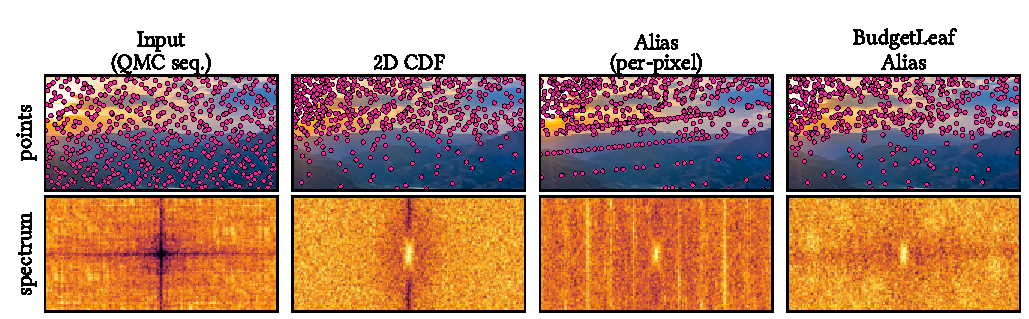
\includegraphics[width=\columnwidth]{fig_qmc_points.pdf}
  \caption{\newmat Top: the first 500 points of the Halton sequence (bases 2, 3), as input and after each warp, over a $1024{\times}512$ region of the Cinema texture. Bottom: power spectrum of the first 60000 points. The per-pixel alias table uses the table construction of our renderer; BudgetLeafAlias uses 4000 leaves.}
  \label{fig:qmcpoints}
\end{figure}

\paragraph{What it costs in a rendering.}
We render a diffuse floor lit by the textured area light through a fence (direct lighting, light sampling only, no MIS), with the Halton set and an independent toroidal shift per pixel, against an exact reference obtained by quadrature over the emitter (Figure~\ref{fig:qmcfence}, Table~\ref{tab:qmc}). With pseudorandom numbers the samplers are equal, as their densities predict. With QMC input the 2D CDF becomes 3.5 times better and the per-pixel alias table 2.6 times \emph{worse}, while LeafAlias stays at its pseudorandom level. The per-pixel alias table with QMC does not converge at all between 128 and 512 samples per pixel, where the stride is 4, 2 and 1 rows (relative RMSE 0.145 and 0.143 on the unoccluded part of the floor, against 0.054 and 0.025 for LeafAlias and 0.013 and 0.004 for the 2D CDF), and starts to fall only at 1024 samples.

\begin{figure}[htbp!]
  \centering
  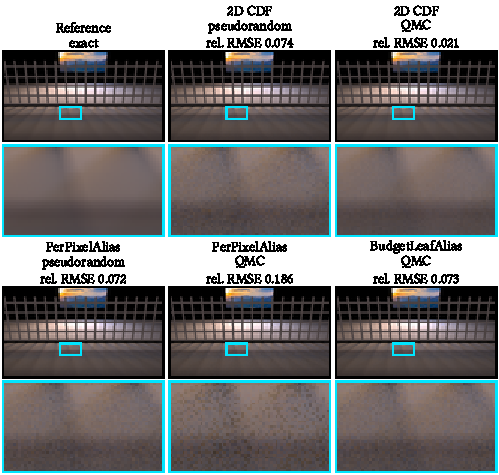
\includegraphics[width=0.92\columnwidth]{fig_qmc_fence.pdf}
  \caption{\newmat A diffuse floor lit through a fence by the emitter of Figure~\ref{fig:qmcpoints}, at 128 samples per pixel: exact reference; 2D CDF with pseudorandom and QMC input; per-pixel alias table with pseudorandom and QMC input; BudgetLeafAlias with QMC input. Close-ups below each render.}
  \label{fig:qmcfence}
\end{figure}

\begin{table}[htbp!]
\centering\small\newmat
\caption{\newmat Top: relative RMSE of the scene of Figure~\ref{fig:qmcfence} at 128 samples per pixel. Bottom: ratio of the QMC error to the sampler's own pseudorandom error over 2406 emitters and emitter regions (photographs, video frames, sky images and windows of our textures), one shading point behind six kinds of occluder.}
\label{tab:qmc}
\begin{tabular}{lcc}
\toprule
Relative RMSE, 128 spp & Pseudorandom & QMC \\
\midrule
2D CDF & 0.074 & 0.021 \\
Per-pixel Alias & 0.072 & 0.186 \\
BudgetLeafAlias (4000 leaves) & 0.074 & 0.073 \\
LeafAlias (1000 leaves) & 0.075 & 0.072 \\
\midrule
QMC error / own pseudorandom & 128 spp & 1024 spp \\
\midrule
Per-pixel Alias, median & 0.92 & 0.79 \\
\quad cases above 1.10 & 16.7\% & 7.3\% \\
\quad worst case & 1.85 & 3.51 \\
BudgetLeafAlias, median & 0.99 & 0.93 \\
\quad cases above 1.10 & 0.0\% & 0.5\% \\
\quad worst case & 1.10 & 1.20 \\
\bottomrule
\end{tabular}
\end{table}

This is not a property of one region: of 225 overlapping $1024{\times}512$ windows of the same frame, the per-pixel alias table with QMC is worse than with pseudorandom numbers in 131, and it is worse in 65\% of the 40 flat sky photographs we tested. Over 2406 emitters (Table~\ref{tab:qmc}, bottom), the QMC error of BudgetLeafAlias stays within 10\% of its own pseudorandom error in more than 99\% of the cases, whereas the per-pixel alias table exceeds that bound in 7--17\% of the cases and reaches 3.5 times. These magnitudes are a best case for QMC, a single two-dimensional direct-lighting integral; in a full path tracer both the gain of the 2D CDF and the loss of the per-pixel alias table are smaller.

\paragraph{Scope.}
A table over a few thousand leaves, each covering many texels, has no fixed relation between bucket stride and image position, so it creates no pattern; but it does not preserve the low-discrepancy distribution either, and its QMC and pseudorandom errors are the same. The 2D CDF and hierarchical warps do preserve it, at the memory and per-sample cost reported in Section~\ref{sec:cost}, and the 2D CDF remains the lowest-error sampler under QMC when that cost is not a concern. On emitters that do not trigger the pattern, among them the five videos of this paper, the per-pixel alias table with QMC input had lower error than LeafAlias. The advantage of LeafAlias here is predictability: its error does not depend on whether the pattern conditions are met. The \supp{qmc\_note}, with its code, reproduces these figures and tables and adds a convergence study.
\newend

\section{\texorpdfstring{\newt{Temporal stability}}{Temporal stability}}
\label{app:temporal}

\newbegin
We evaluate temporal stability on 60 consecutive frames of each scene, rendered at equal samples with a new random seed every frame, against a converged reference for every frame. With $I_t$ the render and $R_t$ the reference of frame $t$, the \emph{temporal error} is
\begin{equation}
E_T = \sqrt{\left\langle\left[(I_t - I_{t-1}) - (R_t - R_{t-1})\right]^2\right\rangle},
\end{equation}
averaged over pixels and frames: subtracting the reference's own change removes what the video itself does, so only change introduced by the renderer remains. The \emph{low-frequency temporal error} is the same quantity after a Gaussian blur with $\sigma = 8$ pixels, which averages out per-pixel noise and keeps the kind of change that is seen as flicker, regions pulsing or popping between frames. Independently of rendering, we measure how much the sampling density changes between consecutive frames with the Jensen--Shannon divergence.

\paragraph{The coarser density changes less.} A per-texel density follows every change of the video, including compression noise, grain and small moving details. A leaf density averages each region over many texels, so these small changes largely cancel, and a leaf boundary that moves between frames only reassigns probability between neighbouring leaves of similar radiance. The density of BudgetLeafAlias changes 5.4, 2.5, 2.5 and 1.8 times less than the exact one in Rover, Cinema, Phone and Convergence, and about the same in Fireplace Room (Figure~\ref{fig:temporal}, left), even though 3--13\% of the $8{\times}8$ cells change leaf size every frame.

\begin{figure}[t]
  \centering
  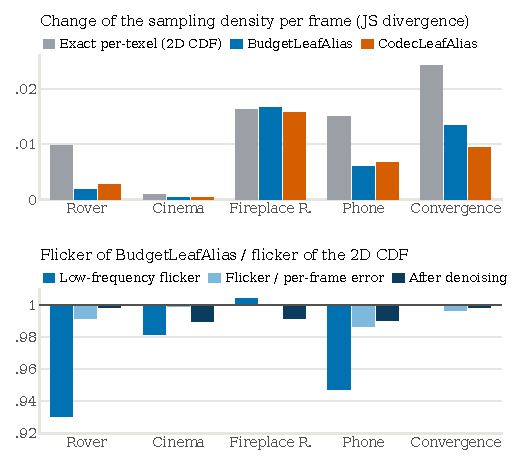
\includegraphics[width=\columnwidth]{fig_temporal.pdf}
  \caption{\newmat Top: change of the sampling density between consecutive frames, for the exact per-texel density (the 2D CDF's) and for the two LeafAlias densities. Bottom: rendered flicker of BudgetLeafAlias divided by the 2D CDF's, at equal samples; below 1 means less flicker.}
  \label{fig:temporal}
\end{figure}

\paragraph{Rendered flicker.} The low-frequency temporal error of BudgetLeafAlias is lower than the 2D CDF's in Rover, Cinema and Phone (7\%, 2\% and 5\% less) and the same in Fireplace Room and Convergence; that of CodecLeafAlias is within 0.0002 of the 2D CDF's in every scene (values of 0.0026--0.0072). The standard deviation over frames of the mean error of the whole frame (brightness pumping) is the same for all techniques. The full temporal error includes the per-pixel noise of each frame, so it grows with the per-frame error: BudgetLeafAlias is equal to or below the 2D CDF in Rover, Cinema and Phone and 4\% above it in Fireplace Room and Convergence, the two scenes where its per-frame RMSE is also 4--5\% higher. Divided by the per-frame RMSE, its temporal error is lower than the 2D CDF's in all five scenes: the partition changes add nothing measurable beyond the per-frame noise. After the OptiX denoiser, the temporal error of BudgetLeafAlias is equal to or lower than the 2D CDF's in every scene (Figure~\ref{fig:temporal}, right).

\paragraph{Frozen noise.} As a diagnostic, we also froze the random numbers (same seed every frame, no camera jitter), so that the image changes only through the video and the sampling structure. In that setting, where noise no longer hides it, the changing partition is visible as a fine-grained per-pixel change 1.5--3.6 times larger than the 2D CDF's, and a hierarchical warp over the same leaves brings it to 1.03--1.32 times. This setting does not occur in normal rendering, where a new seed every frame makes this change part of the per-frame noise, but it matters for techniques that reuse random numbers across frames, which we did not evaluate. The \supp{temporal\_stability} contains the complete tables.
\newend

\end{document}
"
\ifdefined\cleancopy\highlightfalse\fi
\ifhighlight
  \definecolor{newcolor}{RGB}{0,84,216}
  \definecolor{revcolor}{RGB}{226,106,0}
\else
  \definecolor{newcolor}{RGB}{0,0,0}
  \definecolor{revcolor}{RGB}{0,0,0}
\fi
\newcommand{\new}[1]{{\leavevmode\color{newcolor}#1}}
\newcommand{\rev}[1]{{\leavevmode\color{revcolor}#1}}
\newcommand{\newbegin}{\begingroup\color{newcolor}}
\newcommand{\newend}{\endgroup}
\newcommand{\newmat}{\color{newcolor}}
\newcommand{\revmat}{\color{revcolor}}
\DeclareRobustCommand{\newt}[1]{\textcolor{newcolor}{#1}}
\DeclareRobustCommand{\revt}[1]{\textcolor{revcolor}{#1}}
%% ---------------------------------------------------------------------------
%% Aspirational results (DRAFT ONLY): 
%%   \aspirational{text}            target text or value (magenta) followed by an [ASPIRATIONAL] tag
%%   \aspirational[note]{text}      same, with a note for whoever works on reaching the target
%%   \aspnote{note}                 the tag alone, for captions of tables and figures
%% Search this file and table_video_all.tex for "\asp" to list them.
%% ---------------------------------------------------------------------------
\definecolor{aspcolor}{RGB}{200,0,120}
\DeclareRobustCommand{\aspnote}[1]{{\leavevmode\color{aspcolor}\textsf{\bfseries[ASPIRATIONAL\if\relax\detokenize{#1}\relax\else: #1\fi]}}}
\newcommand{\aspirational}[2][]{{\leavevmode\color{aspcolor}#2}\,\aspnote{#1}}
%% Value inside a table cell: colour only, the note goes in the caption.
\newcommand{\aspcell}[1]{{\color{aspcolor}#1}}
%% Name of a document of the supplementary material.
\newcommand{\supp}[1]{supplementary document \texttt{#1}}

%%
%% The abstract is a short summary of the work to be presented in the
%% article.
\begin{abstract}
We present a method for fast importance sampling HDR textured lights that allows real-time video-driven lighting.
Our method partitions a light's texture into a budgeted, variance-driven quadtree and builds an alias table over the resulting leaves, avoiding the cost of a dense per-frame CDF while still capturing
the texture's overall energy distribution. We present two variants: one that reuses the per-frame hierarchical partitions already present in the metadata of modern video codecs, and another that builds a budgeted quadtree to fit the entire sampling structure in the L1 cache of the GPU. Compared to the dense 2D CDF-inversion baseline, at a matched real-time
frame-time budget our technique reduces RMSE by 9–53\% depending on
scene, by letting the saved sampling cost be reinvested in additional light
samples. \new{With the same number of samples, our technique doesn't introduce considerable error compared to 2D CDF, and delivers up to 3 times faster.}
It also reduces memory consumption and transfers by several orders of magnitude when compared to state-of-the-art samplers.

\end{abstract}

%%
%% The code below is generated by the tool at http://dl.acm.org/ccs.cfm.
%% Please copy and paste the code instead of the example below.
%%
\begin{CCSXML}
<ccs2012>
<concept>
<concept_id>10010147.10010371.10010382.10010385</concept_id>
<concept_desc>Computing methodologies~Image-based rendering</concept_desc>
<concept_significance>500</concept_significance>
</concept>
<concept>
<concept_id>10010147.10010371.10010395</concept_id>
<concept_desc>Computing methodologies~Image compression</concept_desc>
<concept_significance>500</concept_significance>
</concept>
<concept>
<concept_id>10010147.10010371.10010372.10010374</concept_id>
<concept_desc>Computing methodologies~Ray tracing</concept_desc>
<concept_significance>500</concept_significance>
</concept>
</ccs2012>
\end{CCSXML}

\ccsdesc[500]{Computing methodologies~Image-based rendering}
\ccsdesc[500]{Computing methodologies~Image compression}
\ccsdesc[500]{Computing methodologies~Ray tracing}

%%
%% Keywords. The author(s) should pick words that accurately describe
%% the work being presented. Separate the keywords with commas.
\keywords{Image-based lighting, video codecs, Alias tables, emissive textures, real-time rendering }

\begin{teaserfigure}
  \centering
  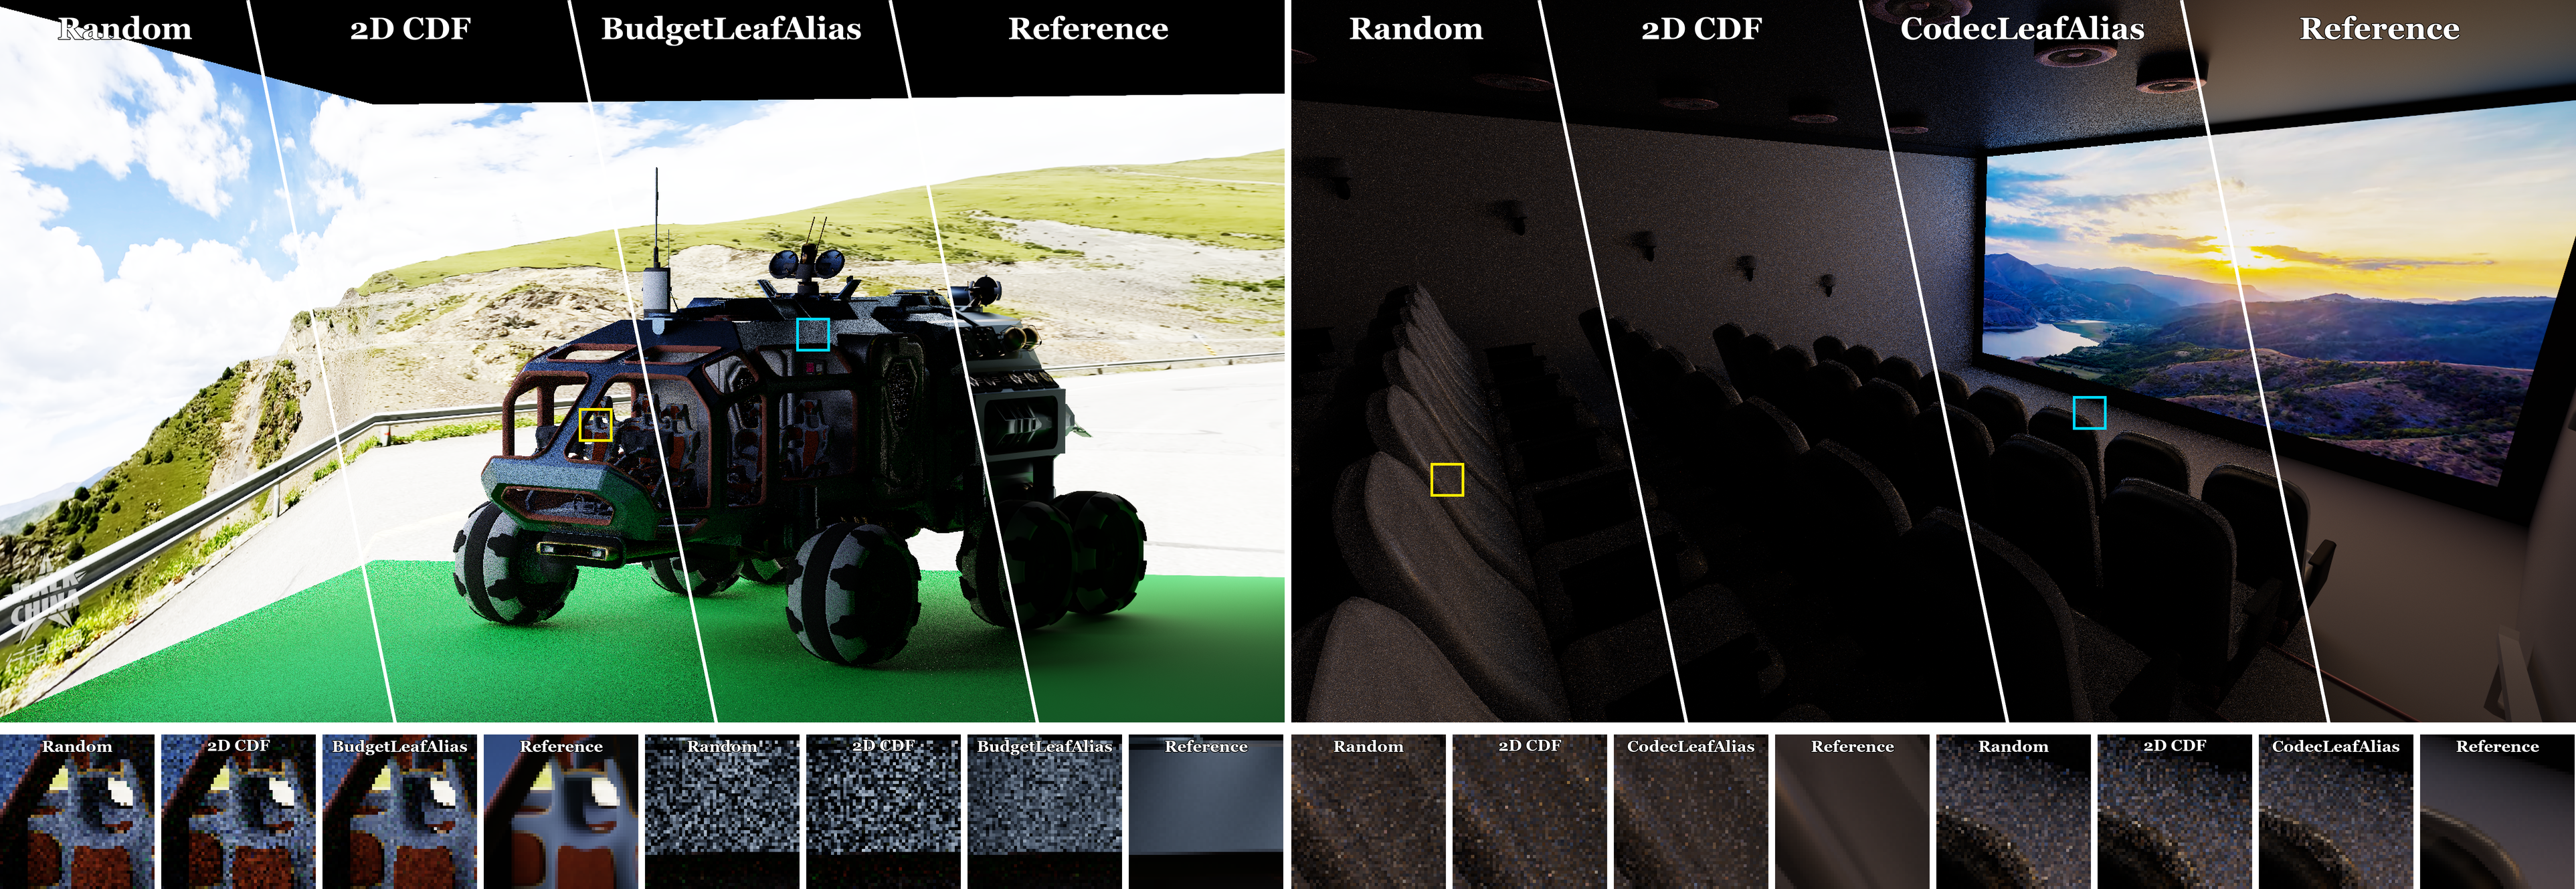
\includegraphics[width=1\textwidth]{teaser.png}
  \caption{Two scenes lit by a single dynamic, video-driven emissive texture, rendered with our LeafAlias importance sampler. (Left) The Rover scene — a virtual-production LED wall displaying a looping road/mountain video panorama that lights the vehicle directly, sampled here with BudgetLeafAlias. (Right) The Cinema scene — a theater lit only by the animated sunset footage playing on its own screen, sampled with CodecLeafAlias. Each panel compares, left to right: Random sampling, 2D CDF inversion, our technique, and a converged reference, all at their calibrated real-time budgets ($\approx$33 ms).}
  \label{fig:teaser}
\end{teaserfigure}

%%
%% This command processes the author and affiliation and title
%% information and builds the first part of the formatted document.
\maketitle

\section{Introduction}

Importance sampling of emissive textures is essential for efficient image-based lighting, and increasingly critical in production and VFX workflows where video is used directly as a dynamic light source. A single emissive texture lets a renderer reproduce the directional detail of a real environment far beyond what analytic lights can approximate. Traditionally, this texture has been static: captured once and reused for an entire sequence. However, there are recent use cases such as LED-wall virtual production, AR/VR object insertion, and video-based environment maps that require illumination that changes every frame.

\rev{The texture light samplers found in current renderers are designed for static images.} They rely on offline construction of large sampling structures that are stored and reused. The most common example of this strategy is how rendering and ray tracing toolboxes deal with HDR environment maps. The standard approach is to build a two-dimensional piecewise-constant distribution from the texture's luminance: a marginal CDF over rows and a per-row conditional CDF. The sampler is then inverted via binary search at sample time, which is expensive and produces incoherent memory access. A more recent and well-adopted approach is to generate a mipmap-style hierarchical importance map \cite{clarberg2005wavelet}. At sample time, a hierarchical descent through a mip pyramid
of the texture is performed, recursively choosing one of four children at each level in proportion to their summed weight. This technique is also expensive and requires several iterations per sample, although it is more GPU-friendly because the number of iterations is always the same for each sample, unlike with the binary search. Moreover, the mipmap can be constructed quickly using the existing dedicated hardware on modern GPUs. Both techniques require at least $O(N)$ memory for the sampler, with $N$ being the number of pixels.

Another less used but known technique for sampling emissive textures is the Alias method \cite{burke2004bidirectional}. This technique draws from an arbitrary discrete distribution in $O(1)$ time after an $O(N)$ one-time build, at the cost of losing the CDF's implicit spatial coherence: two adjacent table buckets can alias to two arbitrary, unrelated locations in the original distribution. This fact is known to disrupt stratification or discrepancy reduction of the input point set. It also requires $O(N)$ memory to store the correlation between every pixel. The process for building the Alias table, despite being $O(N)$, is difficult to optimize for real-time construction \cite{lehmann2021weighted}.

We present a new sampling method that is fast to build, produces a sampler that is tiny, \rev{is $O(1)$ to sample, and does not create the structured sample patterns that the per-pixel Alias method can produce.} The core idea is to reuse the variance-driven image partition that is already present in modern video codecs, which already compute hierarchical spatial partitions that adapt to local signal variance \cite{uhrina2024performance}. These structures implicitly encode the spatial distribution
of luminance and high-frequency content (see Fig. \ref{fig:quadtree}). We also propose a variant that builds the partition tree on a budgeted number of leaves, using a  Greedy/best-first tree-structured resource allocation strategy \cite{MINASNY2007383,Zhou2024}. \rev{Both techniques render video light textures in real time (33 milliseconds per frame) with consistent gains, because each of their samples is cheaper and more of them fit in the frame.}

\newbegin
Our samplers are per frame by design: each frame's structure is built from that frame alone, with no knowledge of past or future frames. Their purpose is not to sample a frame more accurately than an exact per-texel distribution, which is not possible, but to approach its accuracy with a structure that is orders of magnitude smaller and cheaper to build and to sample. Our contributions are:
\begin{itemize}
\item LeafAlias, an alias table over the leaves of a variance-driven partition of the texture, with $O(1)$ sampling and an $O(1)$ density lookup for multiple importance sampling, in a structure of tens of kilobytes.
\item Two sources for the partition: the coding tree of a video codec, with a study of how leaf radiance is obtained from coded data and how quantization, bitrate, codec family and encoder configuration affect it; and a greedy quadtree with a fixed leaf budget.
\item An evaluation that separates the quality of the sampling density (equal samples) from its cost (equal quality), over full videos and against per-texel baselines, together with studies of the leaf budget and its relation to the GPU cache, of static against per-frame partitions, and of temporal stability.
\end{itemize}
\newend

\begin{figure}[htbp!]
  \centering
  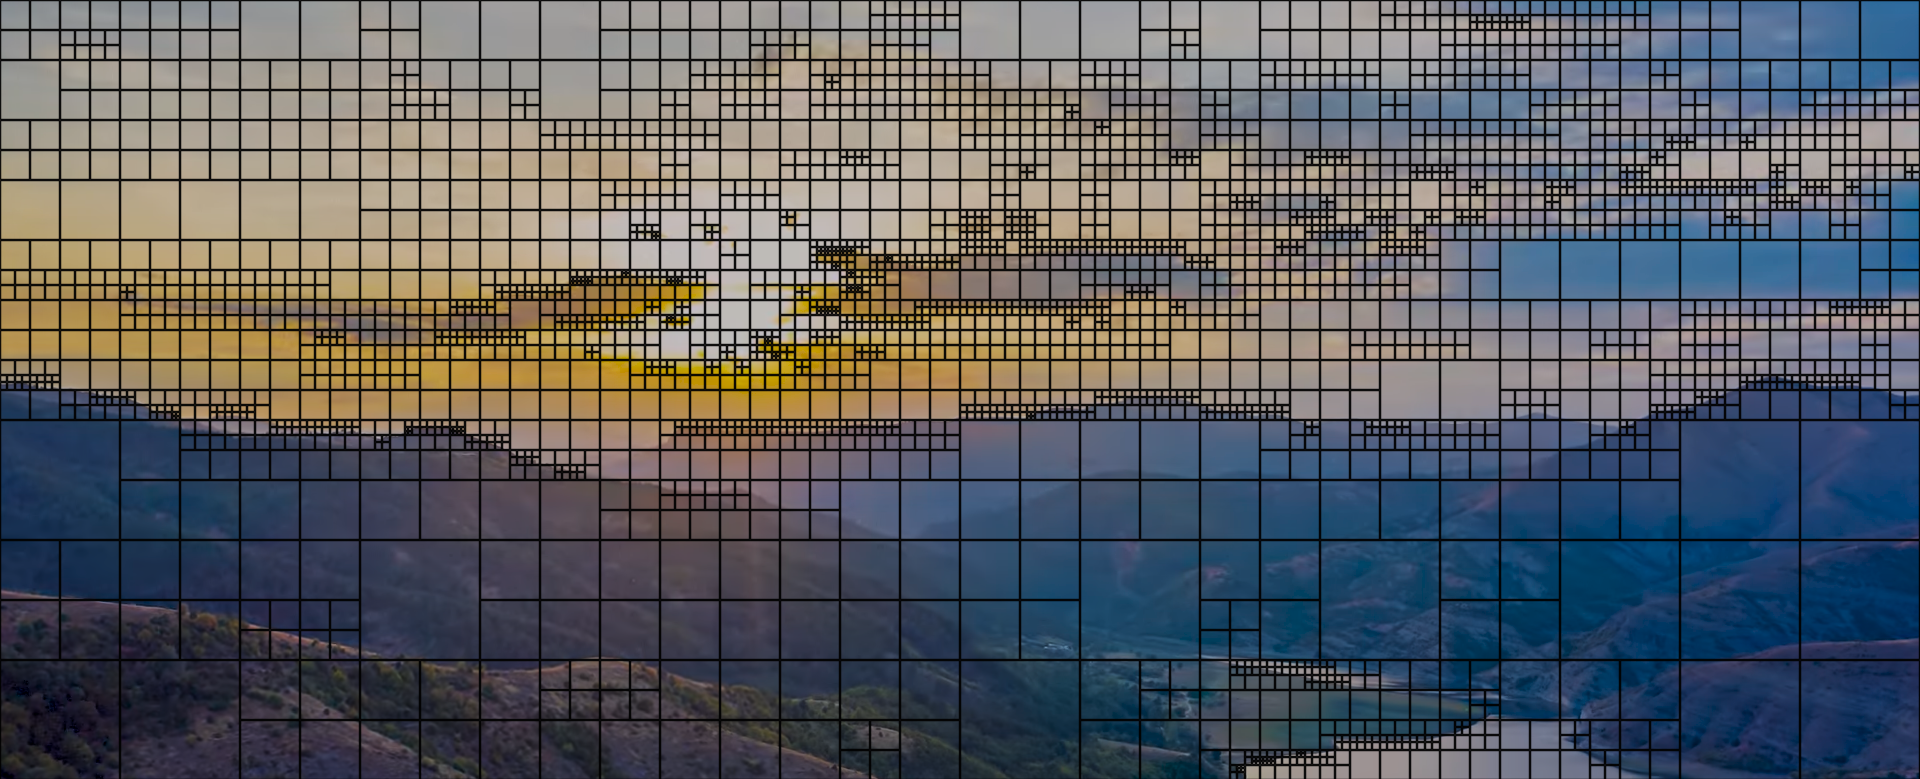
\includegraphics[width=\linewidth]{quadtree.png}
  \caption{An example of a variance-driven quadtree built by the VP9 video codec. High-variance zones are refined into a dense mesh of
  small cells.}
  \label{fig:quadtree}
\end{figure}

\new{
\section{Motivation}

\paragraph{Real-time path tracing in games.}
Light sampling with spatiotemporal resampling draws its initial candidates from
tabulated distributions over emissive geometry and environment maps
\cite{bitterli2020spatiotemporal}, and the cost of rebuilding those tables is a known
obstacle to dynamic content. Wyman and Panteleev~\cite{wyman2021rearchitecting} report the cost of
alias-table builds for large environment maps as one of the main challenges in presampling lights, and instead propose
a GPU-accelerated MIP structure to process textures coming from light probes streamed live from a 360 camera. The quality
of these initial candidates still bounds the result and limits resampling \cite{zeng2025restirpg}, and the integration
of ReSTIR in a shipped path-traced game lists initial candidate sampling quality among
its main sensitivities, with emissive surfaces and the skylight left to BSDF sampling
\cite{kozlowski2023cyberpunk}. Production engines report the same pressure from
content. Lumen lights scenes with emissive surfaces but notes how small
and bright areas cause noise artifacts, and names
explicit sampling of emissive meshes as future work \cite{wright2022lumen}; its
successor for direct lighting observes that artists now use rectangular and textured
lights more frequently \cite{narkowicz2025megalights}. Current guidance for path-traced
games recommends environment maps that are baked every frame so that dynamic skies and
clouds can be importance sampled, and a dedicated sampling structure for signs,
animated effects and procedural emissive materials \cite{nvidia2026ptwhitepaper}.
Recent work still describes the evaluation of many lights per pixel as a major
bottleneck of real-time rendering \cite{chen2026lightopt}.

\paragraph{Virtual production.}
On an LED stage the wall is at once the in-camera background and the light source of
the scene: the stage is driven as an image-based lighting instrument
\cite{debevec2022dilation,legendre2022jointly}, and the video that
drives the wall also drives the lighting fixtures around it \cite{bengtsson2022ibl}.
While the camera rolls, the panels light the real actors physically. The rendering
problem appears whenever the subject under that light is synthetic, and this happens
at three points of a production. Before the shoot, the lighting of a volume is designed
in simulation: productions go through a prelight in the virtual art department, where
the engine reproduces the environment as it will appear on the screens
\cite{kadner2023stages,zwerman2023ves}, techvis rebuilds the on-set hardware as a 3D
scene \cite{failes2024hotd}, and digitized performers are previsualized inside the
virtual stage \cite{nash2025integration}. Such previsualization of panel-generated lighting effects is older than the LED volume \cite{bunish2017rogueone,seymour2013gravity,hamon2014gravity}. During the shoot, when a shot cannot be finished
in camera, the camera frustum is keyed and provisional imagery is composited live
while the rest of the wall keeps lighting the subjects \cite{kadner2021fieldguide}.
After the shoot, the creatures and environments of such shots are added in post
\cite{failes2022hotd} and have to match the lighting that the wall gave the actors.
Research has started to treat the wall accordingly, as a near-field, high-resolution
textured emitter whose image is known at every frame \cite{azzarelli2026relightable},
and to use LED stages to reproduce per-frame HDR environment maps at video rate
\cite{zhang2026pixelcube}. In all of these cases a renderer lights a synthetic subject
with a video, and its sampling structure has to follow that video frame by frame.

\paragraph{Mixed reality and telepresence.}
In augmented and mixed reality the illumination is captured
or estimated while the application runs. HDR environment maps are inferred from the
camera feed at interactive rates on mobile devices
\cite{legendre2019deeplight,somanath2021hdr,zhao2021xihe}, estimated consistently over
video \cite{li2023spatiotemporally,shen2025stglight,bolduc2026limo}, or taken directly
from a live $360^\circ$ stream with changing real-world lights
\cite{rhee2017mr360,rhee2018mr360live,walton2018dynamic}. For such high-frequency
illumination, importance sampling of the environment map is essential for efficient
rendering \cite{kronander2015photorealistic,alhakamy2020realtime}. Systems that do
path trace under a live panorama on a head-mounted display report that the result must
be denoised \cite{cheng2023environment,wu2024panoramic}, and that in a headset Monte
Carlo noise is more than a quality problem, since its temporal flicker aggravates
cybersickness \cite{taibo2024immersive}. Most real-time systems therefore avoid
sampling: they prefilter the map or reduce it to a few dominant lights\cite{saito2024relightable}. A sampling structure that can be rebuilt at
the rate of the display, and that is small enough to keep one per light, is a
precondition for moving these applications from prefiltered shading to path tracing
with correct shadows and interreflections.
}
\section{Previous works}\label{sec:prev}
Importance sampling of emissive textures is a well-studied problem in the graphics literature in the context of image-based lighting. Most of the works focus on preprocessing the images to allow for exact or near-exact sampling without introducing bias \cite{lawrence2005adaptive}. Several methods choose to simplify the textured light into a set of point or area lights ~\cite{agarwal2003structured}, allowing for real-time sampling and faster convergence but at the cost of more error in the solution. \cite{cline2009tabular} compare several tabular inversion methods, noting the computational order of building each sampler structure and sampling each point. They analyze the 2D CDF inversion via binary search and the per-pixel Alias method, where they flag the disruption of the stratification of the input point set. \rev{With a low-discrepancy input, the raster-flattened table of the per-pixel Alias method can produce a measurable periodic banding pattern (Figure~\ref{fig:spectrum}) that becomes clear in the power spectrum of the sample set. Appendix~\ref{app:qmc} analyzes these effects and their consequence in a rendering for our proposed methods and compares it with per-pixel Alais.}

\begin{figure}[htbp!]
  \centering
  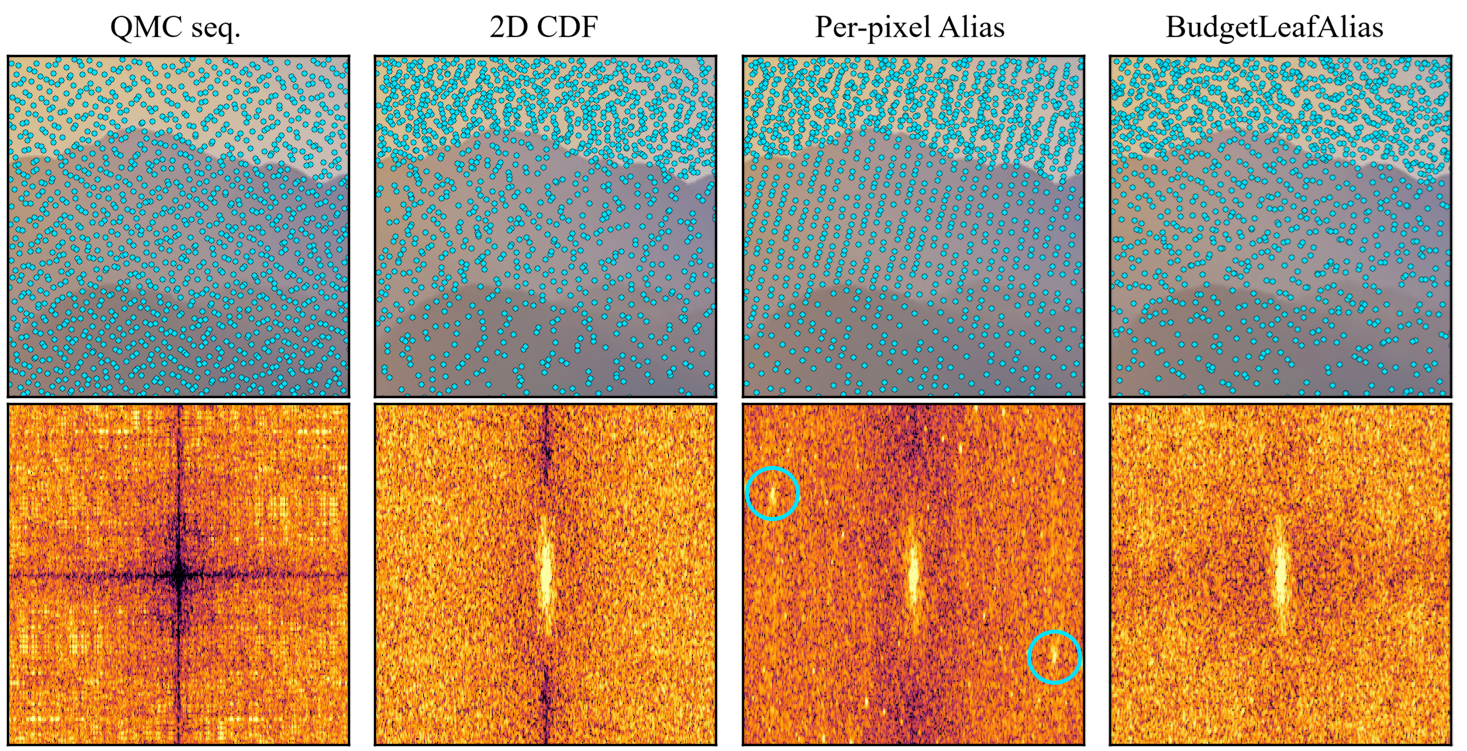
\includegraphics[width=\linewidth]{fig_spectrum_paper_color.png}
  \caption{2D power spectrum of samples from 2D CDF inversion, plain per-pixel alias, and
  our LeafAlias, from the same Halton input. Per-pixel alias shows a sharp,
  isolated off-axis peak (flatness 0.270, peak/median 16{,}113), a periodic banding
  artifact from its flat array index resonating with the input sequence's base-2 digit
  structure.}
  \label{fig:spectrum}
\end{figure}

Despite being $O(1)$ to sample, the Alias method is memory-intensive and expensive to construct via Vose's technique.
Nevertheless, it is widely used in mesh light sampling for geometry with thousands of emissive triangles. \cite{moreau2019dynamic} maintain a light-sampling BVH incrementally across frames for thousands of moving lights.
ReSTIR~\cite{bitterli2020spatiotemporal} resamples across spatial and
temporal neighbors to pick among many dynamic lights at a fraction of the cost of resampling
from scratch. Conty Estevez and Kulla~\cite{contykulla2018adaptive} adaptively split a light
tree per shading point rather than committing to one fixed cut. At that scale of thousands of triangles, a plain alias table over per-triangle flux is common practice
and cheap to rebuild every frame.

Regarding the optimization of the sampling structures,
\cite{ergun2012realtime} split an environment map into a kd-tree via the greedy partition strategy, to a predefined block count, then fit the sorted leaf probabilities with an approximate analytic curve for direct inversion. They report gains in memory compression, higher speed and accuracy than CDF inversion at matched performance for static environment maps. One disadvantage of using kd-trees is that evaluating the pdf of the map direction when sampled from the BRDF in multiple importance sampling (MIS) requires traversing the tree.
 Lambers~\cite{lambers2022parameterization} proposes a fixed-grid sampler and notes that replacing the grid with a variance-driven quadtree might improve their results. \cite{rodriguez2023nenv} train a neural normalizing flow that allows both sampling and evaluating the pdf, showing considerable performance gains at the cost of pre-training the structure for the static map. Wu~\cite{wu2025efficient} also preprocesses the map by dividing the emissive and non-emissive parts into separate structures. \new{Sz\'ecsi et al.~\cite{szecsi2010adaptive} adapt the placement of the samples of an environment map on the GPU, taking the reflectance at the shading point into account as well as the illumination. Sampling densities that depend on the shading point, like \cite{szecsi2010adaptive}, MIS-compensated distributions~\cite{karlik2019mis} or variance-aware guiding~\cite{rath2020variance}, are complementary to our work, which builds a scene-independent density from the texture alone.}

\rev{The previously described techniques focus mainly on preprocessing static images to improve sampling efficiency. Sampling of dynamic environment maps has also been studied.} \new{Wan et al.~\cite{wan2005q2tree} subdivide the sphere into a Q2-tree of quadrilaterals according to illumination importance and generate a temporally coherent set of directional samples for every frame of an environment sequence. Wan et al.~\cite{wan2011spatiotemporal} treat the whole sequence as a spatiotemporal volume and stratify the samples in space and time, and Yang et al.~\cite{yang2014high} extend this line to high-dynamic-range sequences. These methods exploit temporal coherence, and the spatiotemporal ones analyze the sequence as a whole before rendering, which suits recorded content. Our method works on the current frame only, so it applies to live video, and it produces a density that can be sampled and evaluated for MIS inside a path tracer, rather than a fixed set of light directions.} \rev{Other works address video-driven lighting:} \cite{havran2005interactive} and Iorns and Rhee~\cite{iorns2015realtime} both light scenes from captured video environment maps, but neither targets real-time per-frame
resampling of the video itself as the importance distribution. \cite{lu2013realtime} rebuild a tabulated per-cube-face CDF in real-time, noting it as an expensive part of the process. \cite{kronander2014real} rely on temporal sample reuse to improve convergence of video-based lighting.

Attempts to make the per-frame rebuild itself cheaper on a GPU point in the same direction: Morrical and Zellmann~\cite{morrical2021inverse} accelerate 2D CDF
inversion with ray tracing hardware at a high construction cost and non-trivial implementation
complexity. \cite{lehmann2021weighted} study GPU-specific weighted sampling and alias-table construction directly. \new{Binder and Keller~\cite{binder2019radix} build radix tree forests in parallel on the GPU to sample discrete distributions with a monotone mapping. These approaches make a per-texel structure faster to build; ours reduces the size of the structure instead, which lowers the cost of building it, storing it and sampling it at once.}

Modern production renderers mostly rely on dense CDF or mipmapped samplers. {Falcor}~\cite{falcorsoftware} uses a hierarchical mip-pyramid importance map over the environment texture's luminance and, separately,
the triangle-scale alias table for mesh lights. {Mitsuba 3}~\cite{nimierdavid2019mitsuba2} builds a {Hierarchical2D} warp over
the environment map, which is the same mip-pyramid family as Falcor's. {pbrt-v4}~\cite{pharr2023pbrt}
uses a dense CDF distribution, inverted via binary search. {Blender Cycles}~\cite{cyclessoftware} builds the same
kind of dense marginal/conditional CDF over a downsampled background map.

\section{Method}\label{sec:method}

The LeafAlias technique applies to any light source described by a 2D radiance texture $L(u,v)$ over
a parameter domain $(u,v)\in[0,1)^2$, e.g. an environment map, or the emission texture of an
area light. As with any textured light, variance is minimized when the sampling density
matches radiance, $p(u,v)\propto L(u,v)$. We approximate this with a piecewise-constant density
over a partition of the domain into disjoint leaf rectangles $\{R_i\}_{i=1}^N$, for now
assumed given; Sections \ref{sec:codec} and \ref{sec:budget} describe the two ways we
actually construct it. Each leaf carries a single weight proportional to its flux: its area in the parameter domain
times its average radiance:
\begin{equation}
w_i = A_i \bar{L}_i, \qquad \bar{L}_i = \frac{1}{A_i}\int_{R_i} L(u,v)\,dA. \label{eq:weight}
\end{equation}
Normalizing over all leaves gives a piecewise-constant density over the parameter domain
and a per-leaf selection probability:
\begin{equation}
p(u,v) = \frac{\bar{L}_i}{W} \ \text{for } (u,v) \in R_i, \qquad
p_i = \frac{w_i}{W}, \qquad W = \sum_{j=1}^N w_j. \label{eq:pdf}
\end{equation}
Converting $p(u,v)$ to whatever measure a particular light type actually samples with
respect to (solid angle for a distant environment map or projected solid angle for a local
area light) is a standard change-of-variables applied at evaluation time, and is
independent of the sampling structure described below.

Given the partition, we flatten it into an array of $N$ leaves, each storing its rectangle
and weight $w_i$ from Equation~\ref{eq:weight}. We build a Walker/Vose alias
table~\cite{vose1991linear} over this array once, in $O(N)$: leaves below the mean weight
are paired with leaves above it, the excess of the latter absorbs the deficit of the
former, and the process repeats until every leaf holds a threshold and, where needed, the
index of the leaf it aliases to (Algorithm~\ref{alg:build}). Unlike a dense CDF, the
resulting table needs no search at sample time since selecting a leaf is an $O(1)$ array
lookup.

\begin{algorithm}[h]
\caption{Build the alias table over $N$ leaves}
\label{alg:build}
\begin{algorithmic}[1]
\STATE $W \leftarrow \text{mean}(w_1,\dots,w_N)$
\STATE partition leaf indices into \textit{small} ($w_i < W$) and \textit{large} ($w_i \geq W$)
\WHILE{\textit{small} and \textit{large} both non-empty}
  \STATE $s \leftarrow$ pop(\textit{small}); \quad $l \leftarrow$ pop(\textit{large})
  \STATE $\mathit{threshold}[s] \leftarrow w_s / W$; \quad $\mathit{alias}[s] \leftarrow l$
  \STATE $w_l \leftarrow w_l - (W - w_s)$ \COMMENT{transfer $l$'s excess weight to $s$}
  \STATE push $l$ back onto \textit{small} or \textit{large} by its updated $w_l$
\ENDWHILE
\FOR{remaining $i$ in \textit{small} $\cup$ \textit{large}}
  \STATE $\mathit{threshold}[i] \leftarrow 1$
\ENDFOR
\end{algorithmic}
\end{algorithm}

\subsection{Sampling}
\label{sec:sampling}
To draw a light sample, we use three uniform numbers $\xi_1,\xi_2,\xi_3$
(Algorithm~\ref{alg:sample}). $\xi_1$ selects a bucket in $O(1)$;
$\xi_2$ decides whether we keep that leaf or its
alias partner.
$\xi_3$ and $f$ place the sample uniformly
inside the chosen leaf's rectangle. The sample's pdf is read directly from its
leaf's stored average luminance via Equation~\ref{eq:pdf}. Radiance is read from the texture at the sampled $(u,v)$.

\begin{algorithm}[h]
\caption{Draw one light sample}
\label{alg:sample}
\begin{algorithmic}[1]
\STATE $i \leftarrow \lfloor \xi_1 N \rfloor$; \quad $f \leftarrow \xi_1 N - i$
\IF{$\xi_2 < \mathit{threshold}[i]$}
  \STATE $\mathit{leaf} \leftarrow i$
\ELSE
  \STATE $\mathit{leaf} \leftarrow \mathit{alias}[i]$
\ENDIF
\STATE $(u,v) \leftarrow \text{lerp}(R_{\mathit{leaf}}.\mathit{min}, R_{\mathit{leaf}}.\mathit{max},\, (f,\xi_3))$
\STATE \textbf{return} $(u,v)$, $\;p(y){=}\bar{L}_{\mathit{leaf}}/W$ (Eq.~\ref{eq:pdf}), $\;L(u,v)$
\end{algorithmic}
\end{algorithm}

Combining light sampling with BRDF sampling via MIS requires the
reverse query: given a direction chosen by BRDF sampling that happens to hit the light at
some $(u,v)$, the probability $p(y)$ is needed. Rather than searching the partition, we
maintain a small auxiliary lookup matrix that maps a coarsened $(u,v)$ coordinate directly to
its leaf index, at a fixed fraction of the texture's resolution matching the partition's
smallest possible leaf (e.g.\ one entry per $8{\times}8$ block).
Every coordinate covered by a given leaf is written to the same entry at
construction time, so the lookup is an $O(1)$ array read that reproduces the exact same
$\bar{L}_i/W$ used at sampling time regardless of that leaf's actual size, keeping the
resulting MIS weight unbiased. We also tried replacing this exact lookup with a single
scene-wide average density: across our test scenes this produced no perceptible difference
in the rendered images, but it does introduce bias, since the substituted value no longer
matches the technique's actual density at that point.

\subsection{CodecLeafAlias}
\label{sec:codec}
Building the partition can be costly, especially for dynamic content that changes every few milliseconds.
CodecLeafAlias avoids it entirely when the texture
arrives as a compressed video frame. Modern codecs (HEVC, AV1, VP9) already split each frame
into a coding-tree hierarchy driven by local signal variance, which is structurally the same
partition our method needs.
We take each coding-tree leaf's block directly as one of our leaf rectangles $R_i$, and
estimate $\bar{L}_i$ from the block's own zero-frequency (DC) transform coefficient rather
than summing pixels: the DCT/DST's DC term is, up to a fixed normalization constant, exactly
the block's mean sample value, and is already computed and present in decoder metadata.
\newbegin
The DC coefficient gives the mean of a block of the \emph{coded} signal, which for HDR video is a nonlinear, quantized $Y'C_bC_r$ signal (10-bit PQ, BT.2100, in our experiments), so three steps separate it from $\bar{L}_i$. (1)~The reconstructed block mean of each plane is its dequantized DC divided by the transform gain. For a block coded with prediction, the DC belongs to the residual, and the mean of the prediction (extracted from the decoding process) must be added. (2)~The three means are converted to $R'G'B'$ with the BT.2020 matrix, linearized with the PQ transfer function, and transformed to luminance with the BT.2020 weights. (3)~The result is multiplied by the leaf area to give $w_i$ (Eq.~\ref{eq:weight}). This process and quantization perturb the DC, and therefore the density of Eq.~\ref{eq:pdf}, but not the expected value of the estimator: every sample is divided by the density actually used, so the estimate stays unbiased for any density that is positive wherever the emitter is. We keep a small density floor ($10^{-4}$ of the mean weight) so that no lit leaf is quantized to zero. A wrong weight can therefore only add variance; Section~\ref{sec:codecstudy} measures the effect of quantization in the results.
\newend

In our experiments, we encode the dynamic emissive textures as HDR video using libvpx's VP9 Profile 2 and extract the superblocks for each frame via decoder statistics. We configure the encoder to always use variance-based superblock partitioning. Encoder settings that instead search or reuse partitions (full rate-distortion search, predicted neural partitions, etc.) \new{can} still supply a usable partition by combining each block's motion vector with its keyframe's already-computed superblocks. \new{Section~\ref{sec:codecstudy} evaluates this strategy, other codec families and the effect of bitrate.} 

Using codec partitions results in varying number of leaves, ranging from 4000 to 20000 depending on the content. We call this method CodecLeafAlias. Since the sampling algorithms are memory-bound operations, we go further by defining a new partition mechanism that allows us to choose a budgeted number of leaves to reduce memory needs and improve coherence. We call this other method BudgetLeafAlias.

\subsection{BudgetLeafAlias}
\label{sec:budget}
BudgetLeafAlias constructs the quadtree directly from the texture under a hard
leaf-count budget $B$ (in our implementation, matched to what fits alongside the alias
table in a modern GPU's L1 data cache; Section~\ref{sec:impl}). Rather than recursing to a
fixed depth or a fixed per-node threshold, we spend the budget greedily
(Algorithm~\ref{alg:budget}): a priority queue always refines whichever pending block
currently contributes the most summed-squared error to the piecewise-constant
approximation, $\mathrm{Var}(R)\cdot A(R)$, until the budget is exhausted or no block has
positive variance left to resolve. This is the standard greedy construction for a
budget-constrained piecewise-constant approximation: unlike a fixed-depth or
fixed-threshold rule, it spends every one of its $B$ leaves wherever the source image
actually has the most error left to remove.

\begin{algorithm}[h]
\caption{Build a budgeted quadtree of $\leq B$ leaves}
\label{alg:budget}
\begin{algorithmic}[1]
\STATE $\mathit{queue} \leftarrow \{\mathit{root}\}$; \quad $\mathit{leaves} \leftarrow \emptyset$
\WHILE{$\mathit{queue} \neq \emptyset$ and $|\mathit{leaves}| + |\mathit{queue}| + 3 \leq B$}
  \STATE $R \leftarrow$ pop block with max $\mathrm{Var}(R)\cdot A(R)$ from $\mathit{queue}$
  \FOR{each of the 4 children $C$ of $R$}
    \IF{$C$ is $8{\times}8$ texels or smaller, or $\mathrm{Var}(C) = 0$}
      \STATE $\mathit{leaves} \leftarrow \mathit{leaves} \cup \{C\}$
    \ELSE
      \STATE $\mathit{queue} \leftarrow \mathit{queue} \cup \{C\}$
    \ENDIF
  \ENDFOR
\ENDWHILE
\STATE $\mathit{leaves} \leftarrow \mathit{leaves} \cup \mathit{queue}$
\end{algorithmic}
\end{algorithm}

\subsection{Implementation}
\label{sec:impl}
\rev{We implement both variants in NVIDIA's Falcor rendering engine and test using a full path tracer with MIS: one BSDF sample per bounce, and a configurable number of light samples per shading point, each weighted against BSDF sampling.}
We construct the LeafAlias tables and partitions in the CPU, and pass the results to the GPU in each frame.
All the precomputation is done in under 1 millisecond per frame. We implement the sampling method in the Slang Shading Language.
In order to reduce GPU memory usage and improve coherency, we spent some effort in making the sampling structures as small as possible.
Each leaf is packed into a 16-byte record, its rectangle as two packed 16-bit corner coordinates, the alias threshold and redirect index
as a half-float and a 16-bit index, and $\bar{L}_i$ as a half-float. For BudgetLeafAlias, we size $B$ so the combined leaf and node buffers fit within roughly half of the GPU's per-core L1 cache, keeping the whole sampling structure resident there during
traversal instead of round-tripping to global memory on every sample. \rev{With $B=4000$ the structure takes 75\,KB. This compactness helps improve performance when compared to other memory-bound samplers like dense CDF or per-pixel Alias table; Section~\ref{sec:leafbudget} measures the effect of $B$ on quality and on cost.}

\section{Results} \label{sec:results}

All experiments run on an Intel Core i7-14700F CPU and an NVIDIA GeForce RTX 4080 SUPER GPU (128\,kB of L1 cache/shared memory per streaming
multiprocessor). We evaluate seven real-time techniques across our five scenes
(LED-wall Rover, projector-lit Cinema, Fireplace Room, Phone, and the multi-material
Convergence scene): uniform random sampling; dense 2D CDF inversion; the same CDF built at $1/8$ resolution; a hierarchical
mipmap-warp sampler; a per-pixel Alias table; and our
own {BudgetLeafAlias} and {CodecLeafAlias}. We added 2D CDF/8 to analyze the quality and performance
tradeoffs of a coarser resolution; we also tested several further resolution-trimming factors beyond $1/8$ (down to $1/16$ and $1/32$)
and observed the same trend: smaller resolutions are cheaper to sample but significant error is introduced. We report only the $1/8$ variant in what follows, as the representative trimmed-resolution case.

All techniques are implemented in Falcor, with particular
attention paid to making the GPU-side sampling code efficient for each technique. The CPU-side cost
of building each sampling structure for every frame varies considerably: 2D CDF's
dense per-pixel CDF costs approximately $10$\,ms per Full HD frame, while per-pixel Alias table costs approximately $30$\,ms; our own technique's
leaf-budgeted construction is consistently under $1$\,ms per frame across every scene tested. The sampling parameters for each technique (samples per pixel and light samples per vertex) are tuned per scene to a real-time budget of $33$\,ms (30\,fps) using the same calibration procedure. 
 \new{Since we are interested in analyzing the sampler efficiency, not the structures build time, we leave the build time out of the calibration, so the presented real-time results only consider sampling performance. }
2D CDF and mipmapped methods allow approximately a third of the samples obtained with the random approach. BudgetLeafAlias allows the same number of samples as random, while CodecLeafAlias and per-pixel alias allow approximately 25\% fewer. \new{Table~\ref{tab:configs} lists the configurations. BudgetLeafAlias uses $B=4000$ leaves unless stated otherwise.}

\begin{table}[htbp!]
\centering\small\newmat
\setlength{\tabcolsep}{3pt}
\caption{\newmat Calibrated real-time configuration of each technique per scene: samples per pixel $\times$ light samples per shading point, each within the 33\,ms frame. }
\label{tab:configs}
\resizebox{\columnwidth}{!}{%
\begin{tabular}{l ccccccc}
\toprule
Scene & \shortstack{Random} & \shortstack{2D CDF} & \shortstack{2D CDF/8} & \shortstack{Mipmap} & \shortstack{Per-pixel\\Alias} & \shortstack{Budget\\LeafAlias} & \shortstack{Codec\\LeafAlias} \\
\midrule
Rover & 4$\times$19 & 4$\times$5 & 4$\times$12 & 4$\times$9 & 4$\times$13 & {4$\times$19} & 4$\times$15 \\
Cinema & 4$\times$8 & 4$\times$2 & 4$\times$4 & 4$\times$3 & 4$\times$5 & {4$\times$8} & {4$\times$8} \\
Fireplace Room & 4$\times$5 & 4$\times$2 & 4$\times$2 & 4$\times$2 & 4$\times$3 & {4$\times$5} & {4$\times$4} \\
Phone & 16$\times$10 & 16$\times$3 & 16$\times$5 & 16$\times$3 & 16$\times$7 & {16$\times$10} & {16$\times$8} \\
Convergence & 4$\times$3 & 4$\times$1 & 4$\times$2 & 4$\times$1 & 4$\times$2 & {4$\times$3} & {4$\times$3} \\
\bottomrule
\end{tabular}}
\end{table}

Each scene is lit by a different HDR video played back as the
scene's only light source: Rover uses a Full HD road/mountain driving sequence
(600 frames) displayed on a virtual-production LED wall; Cinema uses a Full HD
sunset-landscape sequence (250 frames) with a small, very bright sun; Fireplace Room uses a 4K real fire video (800 frames); Phone uses
a Full HD abstract color sequence (1200 frames); and
Convergence uses a 4K dark cave with multiple bright lights video (800 frames) as a single environment map. Altogether, across these five sequences, our techniques are evaluated against thousands of distinct HDR emissive
textures, not just the one representative frame shown in each figure. The resulting videos are found in the supplementary material.

\new{The evaluation is organized around three questions. Section~\ref{sec:video} reports the quality of every technique over the full videos at its real-time configuration. Section~\ref{sec:equalsamples} removes the cost of sampling from the comparison (equal samples), to measure what the leaf approximation loses. Section~\ref{sec:equalquality} measures what its lower cost gains (time to equal quality). The remaining sections analyze the cost itself, the leaf budget, the need for a per-frame partition, and the codec variant.}

\subsection{\texorpdfstring{\revt{Full-video quality}}{Full-video quality}}
\label{sec:video}

\newbegin
For each scene we render regularly spaced frames spanning the whole video. Each frame is compared with a converged reference of the same frame, without denoising. RMSE is computed per frame on the tone-mapped output and averaged over frames, as well as PSNR; VMAF is computed on the frame sequence of each technique against the reference sequence. We report each mean with its 95\% confidence interval over frames.

Table~\ref{tab:main} reports RMSE, PSNR and VMAF for all seven techniques on all five scenes. On every scene, one of our two techniques has the best mean on all three metrics: BudgetLeafAlias on Rover, Cinema and Phone, CodecLeafAlias on Fireplace Room and Convergence. Relative to the 2D CDF, the best of our two techniques lowers the video RMSE by up to 23\%. The gains hold over the whole video and appear in the perceptual metric as well: on Convergence, VMAF rises from 54.5 with the 2D CDF to 61.5 with CodecLeafAlias.

\begin{table*}[t]
\centering\newmat
\small
\setlength{\tabcolsep}{2.5pt}
\caption{\newmat Full-video RMSE, PSNR (dB) and VMAF for all seven techniques (rows) and all five scenes (column groups), each technique at its real-time calibrated configuration (Table~\ref{tab:configs}). Mean over regularly spaced frames spanning each video, against a per-frame converged reference, with the 95\% confidence interval over frames in small type; PSNR over the frames that have light. Best value per column in bold. \aspnote{the Phone cells of BudgetLeafAlias are targets; measured now 0.0180 / 35.12 / 83.9, with the per-pixel Alias table best on Phone}}
\label{tab:main}
\resizebox{\textwidth}{!}{%
\begin{tabular}{l ccc ccc ccc ccc ccc}
\toprule
\multirow{2}{*}{Technique} & \multicolumn{3}{c}{Rover} & \multicolumn{3}{c}{Cinema} & \multicolumn{3}{c}{Fireplace Room} & \multicolumn{3}{c}{Phone} & \multicolumn{3}{c}{Convergence} \\
\cmidrule(lr){2-4} \cmidrule(lr){5-7} \cmidrule(lr){8-10} \cmidrule(lr){11-13} \cmidrule(lr){14-16}
 & RMSE $\downarrow$ & PSNR $\uparrow$ & VMAF $\uparrow$ & RMSE $\downarrow$ & PSNR $\uparrow$ & VMAF $\uparrow$ & RMSE $\downarrow$ & PSNR $\uparrow$ & VMAF $\uparrow$ & RMSE $\downarrow$ & PSNR $\uparrow$ & VMAF $\uparrow$ & RMSE $\downarrow$ & PSNR $\uparrow$ & VMAF $\uparrow$ \\
\midrule
Random & 0.0524\,{\scriptsize$\pm$.0008} & 25.63\,{\scriptsize$\pm$.12} & 79.4\,{\scriptsize$\pm$1.0} & 0.0640\,{\scriptsize$\pm$.0061} & 24.83\,{\scriptsize$\pm$1.78} & 77.0\,{\scriptsize$\pm$2.8} & 0.1237\,{\scriptsize$\pm$.0014} & 18.16\,{\scriptsize$\pm$.10} & 46.3\,{\scriptsize$\pm$.6} & 0.0194\,{\scriptsize$\pm$.0009} & 34.52\,{\scriptsize$\pm$.39} & 84.1\,{\scriptsize$\pm$.9} & 0.2686\,{\scriptsize$\pm$.0180} & 11.98\,{\scriptsize$\pm$.75} & 42.1\,{\scriptsize$\pm$2.1} \\
2D CDF & 0.0630\,{\scriptsize$\pm$.0007} & 24.02\,{\scriptsize$\pm$.09} & 76.8\,{\scriptsize$\pm$.9} & 0.0666\,{\scriptsize$\pm$.0063} & 24.47\,{\scriptsize$\pm$1.78} & 76.9\,{\scriptsize$\pm$2.8} & 0.0747\,{\scriptsize$\pm$.0006} & 22.54\,{\scriptsize$\pm$.07} & 64.2\,{\scriptsize$\pm$.7} & 0.0180\,{\scriptsize$\pm$.0007} & 35.08\,{\scriptsize$\pm$.33} & 84.1\,{\scriptsize$\pm$.9} & 0.1778\,{\scriptsize$\pm$.0075} & 15.20\,{\scriptsize$\pm$.44} & 54.5\,{\scriptsize$\pm$1.5} \\
2D CDF/8 & 0.0532\,{\scriptsize$\pm$.0008} & 25.49\,{\scriptsize$\pm$.12} & 80.1\,{\scriptsize$\pm$1.0} & 0.0608\,{\scriptsize$\pm$.0057} & 25.22\,{\scriptsize$\pm$1.75} & 78.0\,{\scriptsize$\pm$2.6} & 0.0758\,{\scriptsize$\pm$.0006} & 22.41\,{\scriptsize$\pm$.07} & 63.9\,{\scriptsize$\pm$.9} & 0.0183\,{\scriptsize$\pm$.0008} & 35.01\,{\scriptsize$\pm$.35} & 83.5\,{\scriptsize$\pm$1.1} & 0.1497\,{\scriptsize$\pm$.0056} & 16.65\,{\scriptsize$\pm$.38} & 58.8\,{\scriptsize$\pm$1.2} \\
Mipmap & 0.0557\,{\scriptsize$\pm$.0007} & 25.09\,{\scriptsize$\pm$.11} & 79.3\,{\scriptsize$\pm$1.0} & 0.0631\,{\scriptsize$\pm$.0059} & 24.88\,{\scriptsize$\pm$1.71} & 77.8\,{\scriptsize$\pm$2.7} & 0.0749\,{\scriptsize$\pm$.0006} & 22.52\,{\scriptsize$\pm$.07} & 64.3\,{\scriptsize$\pm$.7} & 0.0180\,{\scriptsize$\pm$.0007} & 35.10\,{\scriptsize$\pm$.33} & 84.2\,{\scriptsize$\pm$1.0} & 0.1786\,{\scriptsize$\pm$.0076} & 15.17\,{\scriptsize$\pm$.44} & 54.2\,{\scriptsize$\pm$1.5} \\
Per-pixel Alias & 0.0528\,{\scriptsize$\pm$.0009} & 25.57\,{\scriptsize$\pm$.15} & 79.5\,{\scriptsize$\pm$1.1} & 0.0610\,{\scriptsize$\pm$.0057} & 25.21\,{\scriptsize$\pm$1.76} & 77.6\,{\scriptsize$\pm$2.7} & 0.0747\,{\scriptsize$\pm$.0006} & 22.54\,{\scriptsize$\pm$.07} & 64.3\,{\scriptsize$\pm$.8} & 0.0179\,{\scriptsize$\pm$.0008} & 35.19\,{\scriptsize$\pm$.35} & 84.2\,{\scriptsize$\pm$1.1} & 0.1461\,{\scriptsize$\pm$.0055} & 16.86\,{\scriptsize$\pm$.38} & 59.1\,{\scriptsize$\pm$1.3} \\
BudgetLeafAlias & \textbf{0.0485\,{\scriptsize$\pm$.0009}} & \textbf{26.30\,{\scriptsize$\pm$.16}} & \textbf{81.1\,{\scriptsize$\pm$1.1}} & \textbf{0.0563\,{\scriptsize$\pm$.0053}} & \textbf{25.89\,{\scriptsize$\pm$1.74}} & \textbf{79.4\,{\scriptsize$\pm$2.5}} & 0.0714\,{\scriptsize$\pm$.0006} & 22.93\,{\scriptsize$\pm$.07} & 65.0\,{\scriptsize$\pm$.7} & \aspcell{\textbf{0.0178\,{\scriptsize$\pm$.0008}}} & \aspcell{\textbf{35.20\,{\scriptsize$\pm$.33}}} & \aspcell{\textbf{84.2\,{\scriptsize$\pm$1.0}}} & 0.1366\,{\scriptsize$\pm$.0048} & 17.42\,{\scriptsize$\pm$.35} & 61.3\,{\scriptsize$\pm$1.2} \\
CodecLeafAlias & 0.0522\,{\scriptsize$\pm$.0010} & 25.66\,{\scriptsize$\pm$.16} & 79.4\,{\scriptsize$\pm$1.2} & 0.0566\,{\scriptsize$\pm$.0053} & 25.84\,{\scriptsize$\pm$1.74} & 78.9\,{\scriptsize$\pm$2.6} & \textbf{0.0708\,{\scriptsize$\pm$.0006}} & \textbf{23.01\,{\scriptsize$\pm$.07}} & \textbf{65.0\,{\scriptsize$\pm$.7}} & 0.0183\,{\scriptsize$\pm$.0008} & 34.97\,{\scriptsize$\pm$.33} & 83.4\,{\scriptsize$\pm$1.1} & \textbf{0.1348\,{\scriptsize$\pm$.0048}} & \textbf{17.54\,{\scriptsize$\pm$.35}} & \textbf{61.5\,{\scriptsize$\pm$1.2}} \\
\bottomrule
\end{tabular}}
\end{table*}


\newend

In order to analyze the real-time performance of each technique, Figure~\ref{fig:realtime} plots the fitted curves of quality as a function of frame processing time. BudgetLeafAlias's curve stays below both structured baselines, 2D CDF and Mipmap for every scene. Its
curve is also consistently the steepest of the three, so the advantage widens as more time
becomes available.

\begin{figure*}[htbp!]
  \centering
  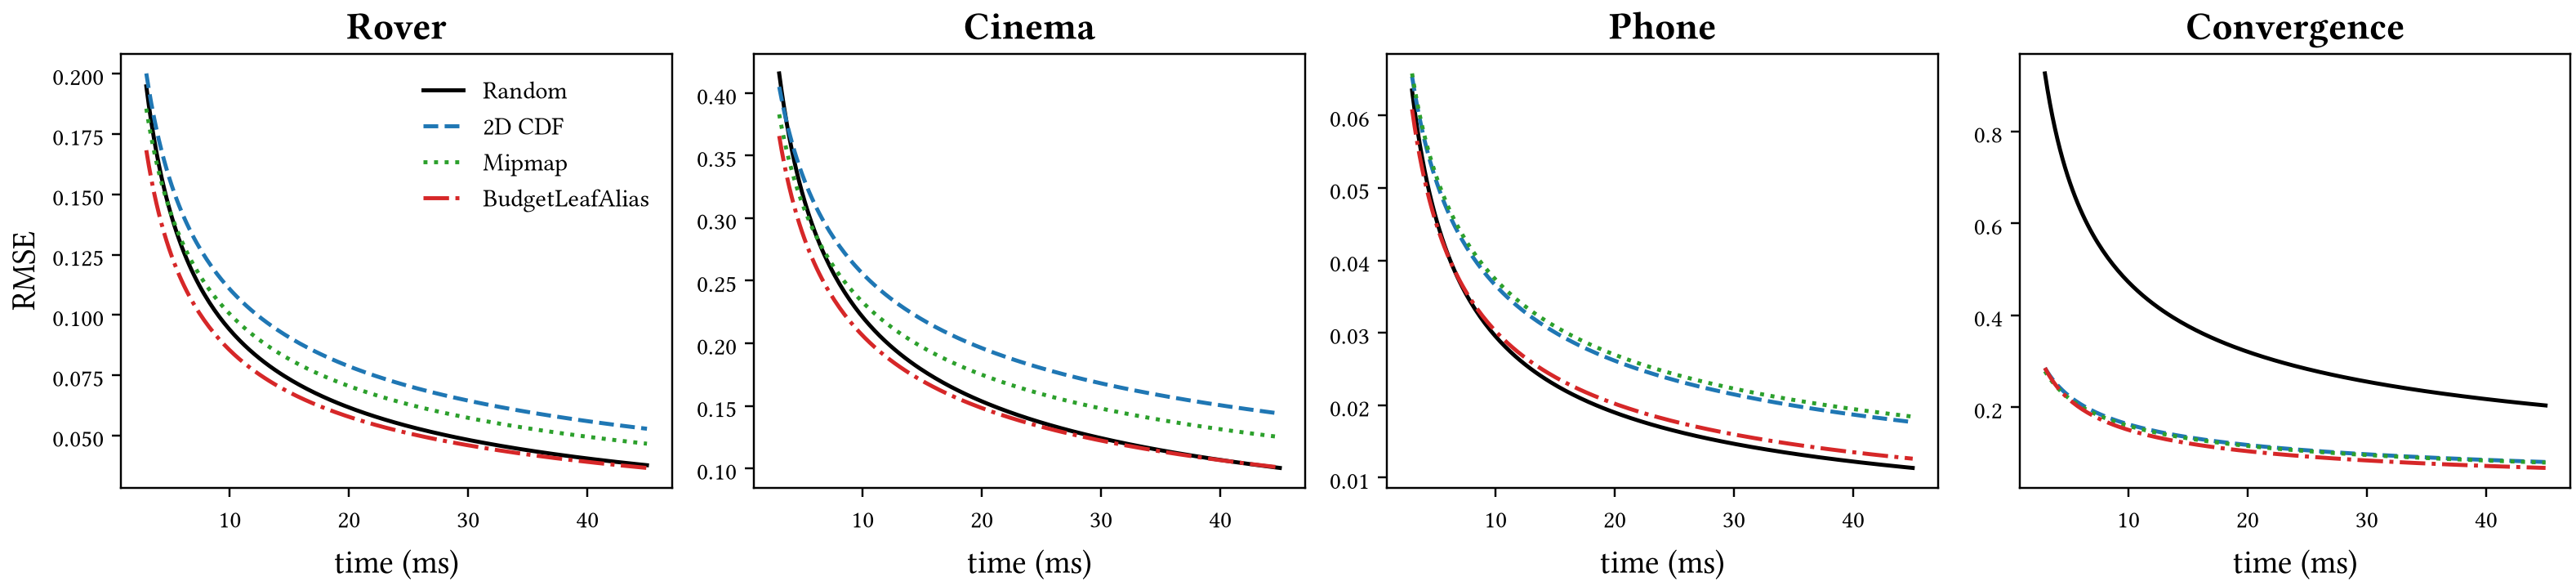
\includegraphics[width=\textwidth]{realtime_curves.png}
  \caption{Fitted RMSE-vs-time curves for Rover, Cinema, Phone, and Convergence, and all four
  techniques. BudgetLeafAlias (red) stays below both 2D CDF
  (blue) and Mipmap (green) across the entire measured range on every scene. }
  \label{fig:realtime}
\end{figure*}

\subsection{\texorpdfstring{\newt{Comparison at equal samples}}{Equal samples}}
\label{sec:equalsamples}

\newbegin
This experiment compares the techniques at the same number of samples for each scene: 4 spp and 2 light samples per vertex. We aim at measuring the variance introduced by using the LeafAlias technique. All techniques render the representative frame of each scene, 24 times with independent random numbers, and the results are compared against a converged reference (Figure~\ref{fig:equalsamples}). The three techniques that importance sample the emitter at full texel resolution (the 2D CDF, the mipmap warp and the per-pixel Alias table) reach the same error within 1\% on every scene. They sample the same distribution and differ only in how they invert it, so at equal samples, and with the independent random numbers of our renderer, they are expected to coincide. Random sampling is clearly worse: its RMSE is 1.12 and 1.21 times that of the 2D CDF on Rover and Cinema, and 1.55, 2.23 and 2.37 times on Phone, Fireplace Room and Convergence. The 2D CDF at $1/8$ resolution is up to 2.6\% behind the full-resolution techniques.

\begin{figure}[htbp!]
  \centering
  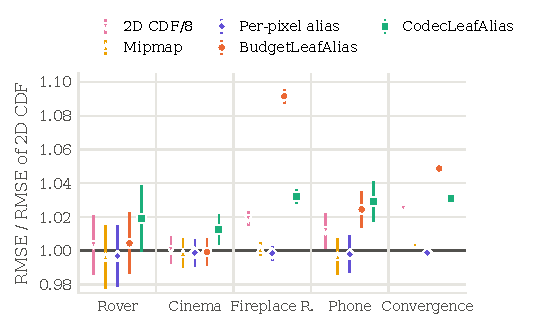
\includegraphics[width=\columnwidth]{fig_equal_samples.pdf}
  \caption{\newmat RMSE of each technique relative to the 2D CDF, with every technique using the same samples per pixel and light samples per shading point (mean of 24 renders, 95\% intervals). Random sampling, at 1.12 to 2.37, is outside the plotted range. }
  \label{fig:equalsamples}
\end{figure}

Our two techniques are slightly behind the full-resolution techniques. Relative to the 2D CDF, the RMSE of BudgetLeafAlias is $+0.4\%$ on Rover, $-0.2\%$ on Cinema, $+2.5\%$ on Phone, $+4.9\%$ on Convergence and $+9.2\%$ on Fireplace Room; that of CodecLeafAlias is $+1.2$ to $+3.3\%$ on all five scenes. The cause is the resolution of the density: both techniques choose a leaf in proportion to its mean luminance and then a point uniformly within the leaf, so the variation of luminance inside a leaf is not importance sampled. CodecLeafAlias has more and smaller leaves on such detailed content and loses less there, but its partition follows image detail rather than light, so it also spends leaves where they do not help. Figure \ref{fig:closeupsequalsamples} shows some rendering closeups for different techniques under the same number of samples.

\begin{figure}[htbp!]
  \centering
  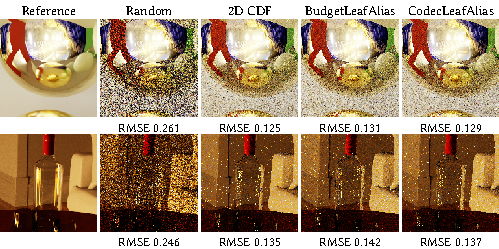
\includegraphics[width=\columnwidth]{closeup_examples.pdf}
  \caption{\newmat Examples of rendering closeups under different techniques with the same number of samples on the Convergence and Fireplace Room scenes.   }
  \label{fig:closeupsequalsamples}
\end{figure}

At equal samples, therefore, our techniques do not sample better than a texel-resolution distribution, and are not meant to: they trade a small loss of sampling quality for a much lower cost per sample and per frame.
\newend

\subsection{\texorpdfstring{\newt{Comparison at equal quality}}{Equal quality}}
\label{sec:equalquality}

\newbegin
In this experiment, we measure how long does each technique need to reach the quality that the 2D CDF delivers in real-time. 
For each scene we render the videos only with direct illumination, where the light sampler controls most of the noise. The 2D CDF uses the number of light samples that fits a 33.3\,ms frame. Every other technique is rendered with several numbers of light samples, and we find the frame time at which its video RMSE equals that of the 2D CDF. The speed-up is the frame time of the 2D CDF divided by that time.

Our two techniques reach the quality of the 2D CDF faster on all five scenes (Table~\ref{tab:equalquality}). These figures use the median frame time of each technique over several timing passes. The other techniques are not consistent: the mipmap warp is slower than the 2D CDF on Rover and does not reach its quality on Phone at the measured sample counts, and the per-pixel Alias table, which is fast on Full HD emitters, is slower than the 2D CDF on the two scenes with 4K emitters, where its memory consumption grows considerably. The time saved can be returned to the frame rate, to more bounces, or to a denoiser.

\begin{table}[htbp!]
\centering\small\newmat
\setlength{\tabcolsep}{3pt}
\caption{\newmat Speed-up of the different techniques over 2D CDF to reach the same average RMSE in the full video.}
\label{tab:equalquality}
\resizebox{\columnwidth}{!}{%
\begin{tabular}{l c c c c c}
\toprule
Technique & Rover & Cinema & Fireplace R. & Phone & Convergence \\
\midrule
2D CDF/8 & 1.17 & 1.89 & 1.29 & 1.17 & 1.17 \\
Mipmap & 0.85 & 1.45 & 1.10 & -- & 1.06 \\
Per-pixel Alias & 1.17 & 1.91 & 0.91 & 1.26 & 0.93 \\
BudgetLeafAlias & 1.31 & 2.23 & 1.19 & \textbf{1.47} & 1.27 \\
CodecLeafAlias & \textbf{1.38} & \textbf{2.31} & \textbf{1.54} & 1.23 & \textbf{1.37} \\
\bottomrule
\end{tabular}}
\end{table}

\paragraph{Emitter resolution}
The last observation suggests that the resolution of the emitter influences the advantage of our techniques. To isolate it, we render using the same emissive texture at three resolutions on the LED wall of the Rover scene: 1820$\times$1024, 3640$\times$2048 and 7280$\times$4096, obtained by area averaging from a real 8K HDR panorama of a road under broad daylight. We render frames with direct illumination, measuring time and RMSE at varying samples per pixel, and smooth the RMSE curve of each technique with a quadratic fit (Figure~\ref{fig:wall}).

\begin{figure}[htbp!]
  \centering
  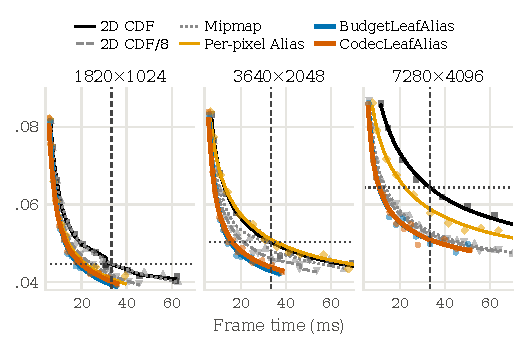
\includegraphics[width=\columnwidth]{fig_wall.pdf}
  \caption{\newmat The same image on the LED wall of the Rover scene at three resolutions: RMSE against frame time (markers: measurements; curves: fits). The vertical line is the 33.3\,ms budget and the horizontal line the RMSE of the 2D CDF at that budget. As the image grows, the curve of the 2D CDF moves to the right and ours stay almost in place.}
  \label{fig:wall}
\end{figure}

The cost of a light sample grows with resolution for the 2D CDF, and much less for our techniques. Each additional light sample per shading point adds 0.95, 1.17 and 2.93\,ms to the frame of the 2D CDF at the three resolutions, and 0.47, 0.50 and 0.73\,ms to that of BudgetLeafAlias. The 2D CDF searches a table as large as the image, with one dependent memory read per search step, and at 8K that table is sixteen times larger than at Full HD; ours read a table of about 75\,KB at any resolution, and the image only once the texel has been chosen. In a 33.3\,ms frame the 2D CDF therefore fits 34, 25 and 10 light samples, while BudgetLeafAlias fits 60, 58 and 40.

As a result, the speed-up at equal quality grows at 8K: both techniques reach the quality of the 2D CDF up to 3$\times$ faster. Read at equal time, the RMSE of BudgetLeafAlias is 12\%, 15\% and 21\% lower than the 2D CDF's. The per-pixel Alias table follows the 2D CDF, since its table also grows with the image and its memory access patterns are more incoherent. The two baselines that keep small or hierarchical structures, the 2D CDF at one eighth of the resolution and the mipmap warp, scale better and reach 2.67 and 2.44 times at 8K; they remain behind our techniques at every resolution. 
\newend

\subsection{\texorpdfstring{\newt{Sampling cost on the GPU}}{Sampling cost on the GPU}}
\label{sec:cost}

\newbegin
We relate the cost of drawing a light sample to the cache levels of the GPU with two benchmarks (Figure~\ref{fig:cache}). In the left figure, a pointer chase reads memory in a chain of dependent random accesses as the working set grows from 4\,KB to 512\,MB. It shows a sharp limit: dependent reads cost about 3\,ps (in aggregate over the whole GPU) while the data fits in the first-level cache, but three times as much once the working set exceeds 128--192\,KB, and tens of times more beyond the second-level cache (64\,MB on our GPU). 

\begin{figure}[htbp!]
  \centering
  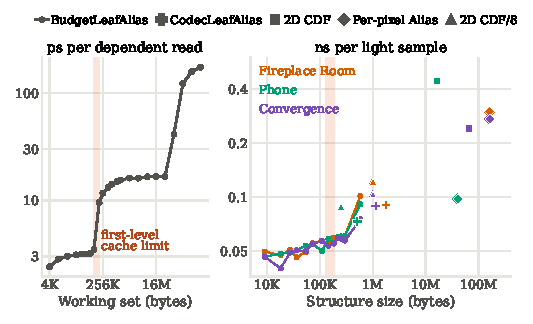
\includegraphics[width=\columnwidth]{fig_gpu_cost2.pdf}
  \caption{\newmat Left: latency of dependent random reads against the size of the data being read, on the GPU (pointer chase, aggregate over the whole GPU). Right: measured cost of one light sample against the size of the sampling structure: BudgetLeafAlias from 64 to 32000 leaves (lines), CodecLeafAlias, and the 2D CDF, per-pixel Alias and 2D CDF/8 (markers), in three scenes. }
  \label{fig:cache}
\end{figure}

In the second figure, we measure the time it takes to draw a sample and read the emissive texture, with varying $B$ values and the other techniques.
The emissive texture read is generally fast because most of the samples point to the same bright sections of the image, hence hitting cache more frequently. These results show the same behavior as the left figure. A sample of the 2D CDF costs between 0.23\,ns and 0.46\,ns, as throughput of the whole GPU, and we give the cost of the other techniques relative to it. BudgetLeafAlias at $B=4000$ is 4 to 8 times cheaper, and its cost hardly changes with the scene; CodecLeafAlias, whose table is larger, costs 1.3 to 1.6 times as much as BudgetLeafAlias. 

The per-pixel Alias table costs a quarter of the 2D CDF on the Full HD emitter of Phone, but 1.2 times as much on the 4K emitter of Convergence. This is explained by the fact that its structure, despite being $O(1)$ to sample, performs two dependent reads per sample at addresses spread uniformly over the whole structure, so almost every read misses the first-level cache; at 4K the structure exceeds the second-level cache as well, and the cost per sample more than doubles.  The 2D CDF performs 24 dependent reads per sample in the worse case, but most of them are cache hits: the marginal CDF is a few kilobytes, and the conditional searches concentrate on the few bright rows.
\newend

\subsection{\texorpdfstring{\newt{Leaf budget}}{Leaf budget}}
\label{sec:leafbudget}

\newbegin
In the next experiment, we sweep the leaf budget $B$ of BudgetLeafAlias from 16 to 16000 leaves in the five scenes at varying number of light samples per pixel. Figure~\ref{fig:leafbudget} shows the error of each budget relative to $B=4000$ at equal samples, so that only the quality of the leaf density is compared.

\begin{figure*}[htbp!]
  \centering
  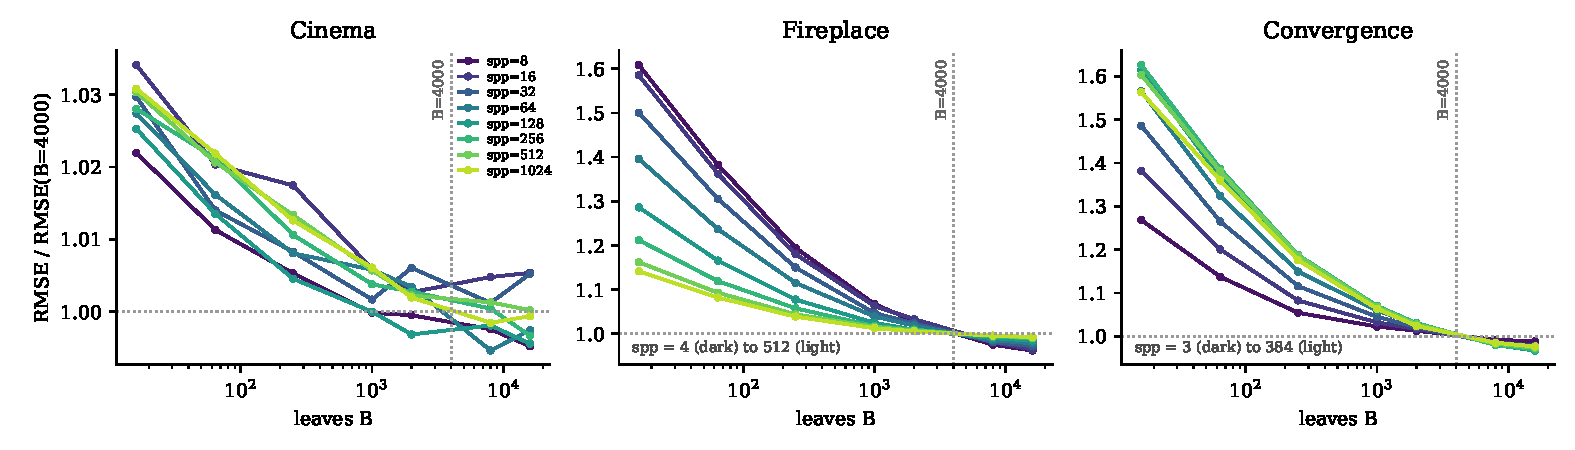
\includegraphics[width=0.92\textwidth]{fig_leaf_budget.pdf}
  \caption{\newmat RMSE against the converged reference, divided by the RMSE of $B=4000$ at the same number of light samples per pixel (spp), as a function of the leaf budget $B$. Values above 1 mean more error than $B=4000$.}
  \label{fig:leafbudget}
\end{figure*}

Two behaviors appear, depending on how the light is distributed over the emitter. In Cinema, light is spread over most of the screen, and a coarse partition already results in one figure error percentages. Rover and Phone behave in a similar way (not shown). In Fireplace Room and Convergence, most of the energy sits in small regions that the partition must resolve, and the error falls steeply with $B$ before levelling off. In Convergence, 250 leaves give up to 1.20 times the error of $B=4000$,  and 1000 leaves up to 1.07 times, while doubling or quadrupling the budget beyond 4000 improves the error by only 1--3\% at every sample count. 

On the cost side, as we saw in the previous section, the structure grows linearly with $B$, and the performance penalty is minimized as long as the sampler resides in L1 cache. $B=4000$ therefore sits at the knee of both curves: it captures nearly all the quality available from the partition, and at 75\,KB it uses most of the cache without exceeding it. $B$ acts as a memory and quality knob, and devices with smaller caches or less memory can use a smaller budget at the quality cost shown in Figure~\ref{fig:leafbudget}. All these measurements are on one GPU; the \supp{ablation\_leaf\_number} contains the complete tables and the  \supp{GPU\_tests} contain results for a mobile GPU device, showing similar patterns when using less cores and memory.
\newend



\subsection{\texorpdfstring{\newt{Frequency of frame partitions}}{Frequency of frame partitions}}
\label{sec:static}

\newbegin
As an alternative to rebuilding the partition every frame, we analyze the error generated by building the tree and leaf weights with less frequency. We compare under equal number of samples: (i)~one tree and one set of weights computed from the average of all frames, with 5\% of the probability spread uniformly to keep the estimator unbiased; (ii)~the same average tree with the weight of each leaf recomputed at each frame; (iii)~a tree rebuilt every 30 frames, with per-frame weights; and (iv)~BudgetLeafAlias. Table~\ref{tab:average-tree} reports the quality of each over the full videos.

\begin{table}[t]
\centering\small\newmat
\setlength{\tabcolsep}{4pt}
\caption{\newmat Quality for static, partially updated and per-frame trees, with 4000 leaves and equal samples per scene (samples per pixel $\times$ light samples per shading point in parentheses). The keyframe tree is rebuilt every 30 frames. The last row of each scene is the ratio of RMSE to BudgetLeafAlias, calculated before rounding. \aspnote{target values; measured now, RMSE ratio: average tree with average weights 1.02--1.40, average tree with per-frame weights 1.002--1.035, keyframe tree 1.00--1.04}}
\label{tab:average-tree}
\resizebox{\columnwidth}{!}{%
\begin{tabular}{l l c c c c}
\toprule
 &  & \shortstack{Avg. tree\\and weights} & \shortstack{Avg. tree,\\per-frame weights} & \shortstack{Keyframe tree,\\per-frame weights} & \textbf{\shortstack{Every frame\\(BudgetLeafAlias)}} \\
\midrule
\textit{Rover} & RMSE $\downarrow$ & 0.0883 & 0.0845 & 0.0842 & 0.0780 \\
(4$\times$2) & PSNR $\uparrow$ & 21.09 & 21.48 & 21.50 & 22.17 \\
 & VMAF $\uparrow$ & 71.0 & 72.0 & 72.1 & 73.4 \\
 & RMSE ratio $\downarrow$ & 1.132 & 1.083 & 1.080 & 1 \\
\midrule
\textit{Cinema} & RMSE $\downarrow$ & 0.0823 & 0.0809 & 0.0825 & 0.0748 \\
(4$\times$1) & PSNR $\uparrow$ & 22.65 & 22.80 & 22.63 & 23.48 \\
 & VMAF $\uparrow$ & 72.8 & 73.3 & 72.9 & 74.6 \\
 & RMSE ratio $\downarrow$ & 1.100 & 1.082 & 1.103 & 1 \\
\midrule
\textit{Fireplace Room} & RMSE $\downarrow$ & 0.1077 & 0.0990 & 0.1008 & 0.0905 \\
(4$\times$1) & PSNR $\uparrow$ & 19.36 & 20.09 & 19.93 & 20.87 \\
 & VMAF $\uparrow$ & 53.8 & 57.4 & 56.9 & 59.2 \\
 & RMSE ratio $\downarrow$ & 1.190 & 1.094 & 1.114 & 1 \\
\midrule
\textit{Phone} & RMSE $\downarrow$ & 0.0353 & 0.0295 & 0.0298 & 0.0272 \\
(4$\times$1) & PSNR $\uparrow$ & 29.38 & 30.93 & 30.83 & 31.63 \\
 & VMAF $\uparrow$ & 79.5 & 80.7 & 80.4 & 81.8 \\
 & RMSE ratio $\downarrow$ & 1.296 & 1.084 & 1.097 & 1 \\
\midrule
\textit{Convergence} & RMSE $\downarrow$ & 0.1866 & 0.1414 & 0.1418 & 0.1268 \\
(4$\times$4) & PSNR $\uparrow$ & 14.70 & 17.11 & 17.09 & 18.06 \\
 & VMAF $\uparrow$ & 50.3 & 60.4 & 60.2 & 62.4 \\
 & RMSE ratio $\downarrow$ & 1.472 & 1.115 & 1.118 & 1 \\
\bottomrule
\end{tabular}}
\end{table}


Rebuilding the tree and its weights every frame gives the lowest error in every scene. A fully static structure raises the RMSE by 10\% on Cinema, 13\% on Rover, 19\% on Fireplace Room, 30\% on Phone and 47\% on Convergence, where VMAF falls by 12 points: fixed weights cannot adapt to changes of the light distribution, and the uniform share spends samples on regions that are dark in a given frame. Recomputing the weights of the average tree every frame recovers most of that loss, but the fixed topology remains 8--12\% behind the per-frame tree, and a tree rebuilt once per second is 8--12\% behind as well.

These results suggest that rebuilding the partition every frame is needed, especially for dynamic content with moving bright spots like the Convergence environment map. The average tree, in addition, requires the whole video in advance, which live and streamed content does not provide, and the per-frame rebuild needs no keyframe interval and adapts at once to cuts, fades and sudden changes of light, where a stale tree is at its worst.

\paragraph{Temporal stability.} Since the partition changes from frame to frame (3--13\% of the $8{\times}8$ cells change leaf size per frame), we measured whether this introduces flicker. Appendix~\ref{app:temporal} gives the metrics and the measurements that show that the leaf density changes \emph{less} between consecutive frames than the exact per-texel density in four of the five scenes, and the low-frequency temporal error of the rendered video, the part perceived as flicker, is equal to or lower than that of the 2D CDF for BudgetLeafAlias in every scene, before and after denoising. 
\newend

\subsection{\texorpdfstring{\newt{Codec partitions}}{Codec partitions}}
\label{sec:codecstudy}

\newbegin

This section analyzes the effect of using the codec partition in CodecLeafAlias as opposed to constructing it based on a leaf number budget. 
Figure~\ref{fig:partitions} shows two examples of partitions, where the codec version is more refined in high-variance parts of the images.
To compare the partitions independently of the renderer, we compute the light-sampling variance factor of the density, $V = \sum_i f_i^2/p_i - 1$, where $f$ is the normalized luminance of the frame and $p$ the sampling density per texel; $V$ is the relative variance of a one-sample estimate of the emitter's power, and is zero for a density proportional to the frame. $V$ isolates the light-sampling part of the error and so changes far more than the rendered error.

\begin{figure}[htbp!]
  \centering
  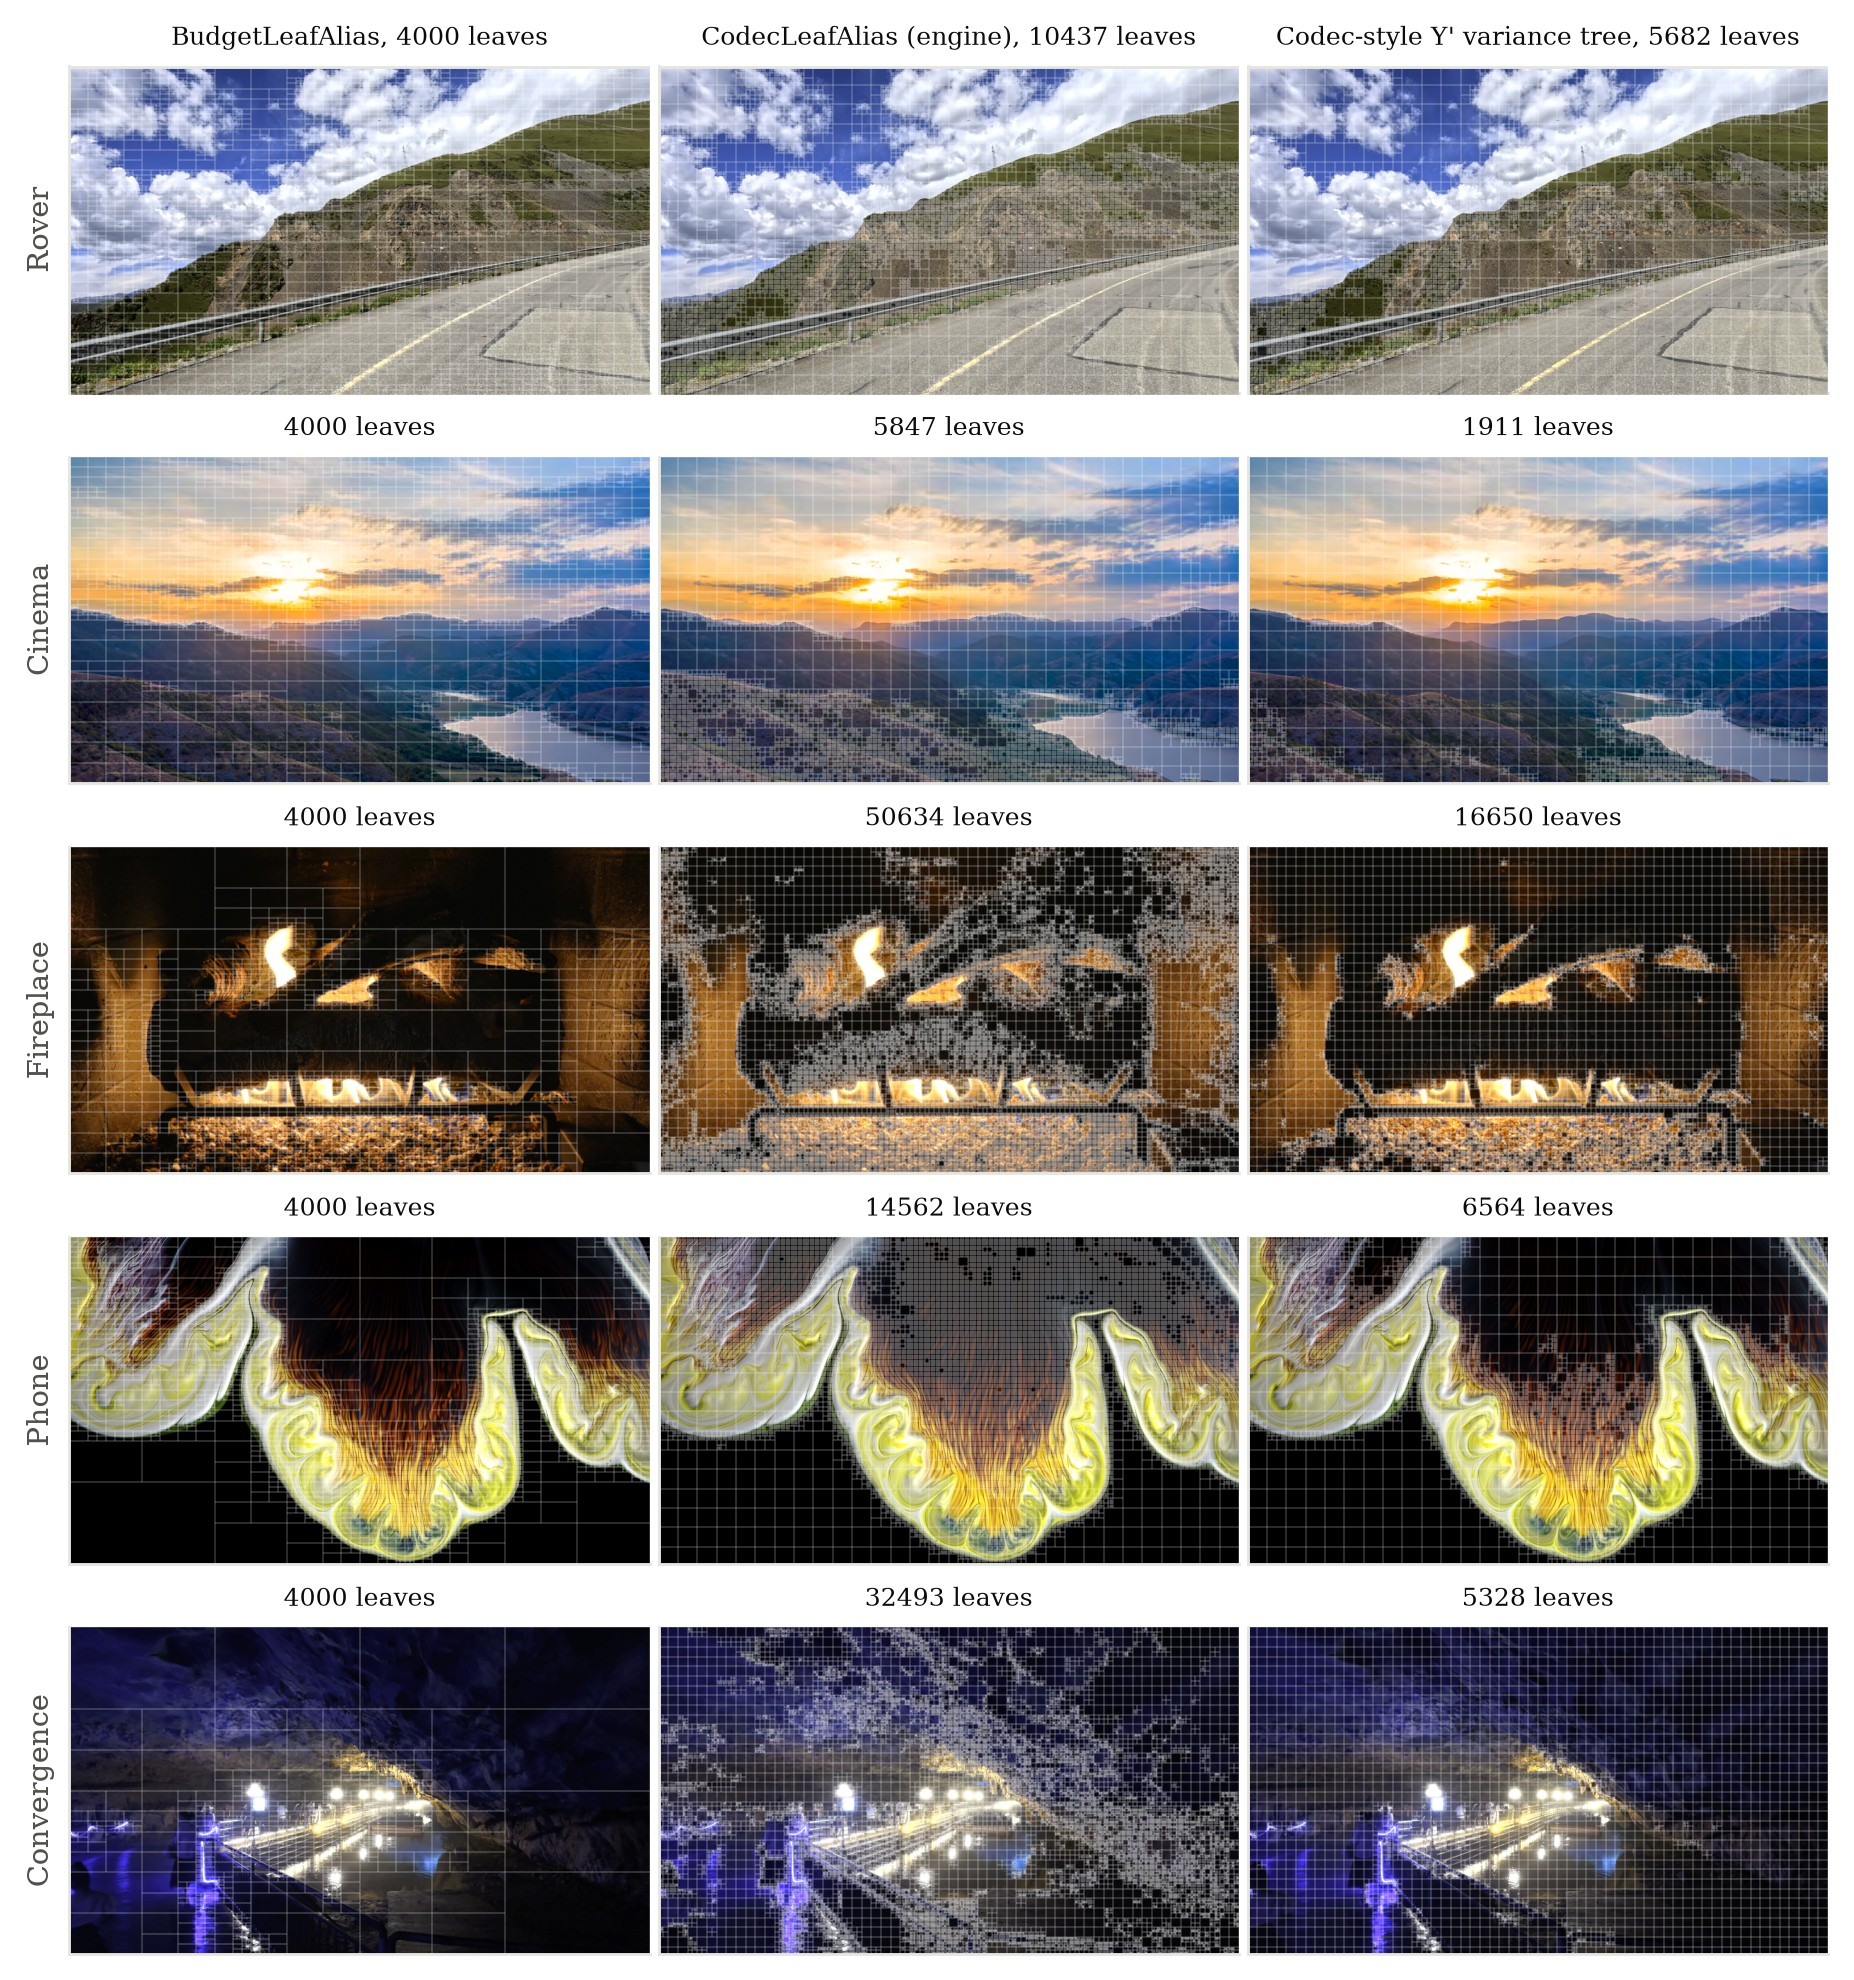
\includegraphics[width=\columnwidth]{fig_partitions.jpg}
  \caption{\newmat Leaf partitions of one frame of Rover and Phone. .}
  \label{fig:partitions}
\end{figure}

Figure~\ref{fig:variance} shows variance against leaf count for BudgetLeafAlias at varying number of leaves, and CodecLeafAlias. 
The plots show that codec leaves are placed less usefully for light sampling in every scene the codec partition lies above the budget curve, and BudgetLeafAlias reaches the same variance with 23--54\% of its leaves (94\% in Phone). A codec partition helps when it has considerably more leaves than the budget: in Fireplace Room it has about 47000 leaves, 12 times the budget, and reaches 0.26 of its variance; in Convergence about 27000 and 0.48. Rendered at equal samples, CodecLeafAlias is accordingly 5.3\% better than BudgetLeafAlias in Fireplace Room and 1.7\% better in Convergence (Figure~\ref{fig:equalsamples}), and it has the best full-video result on those two scenes (Table~\ref{tab:main}). 

\begin{figure}[htbp!]
  \centering
  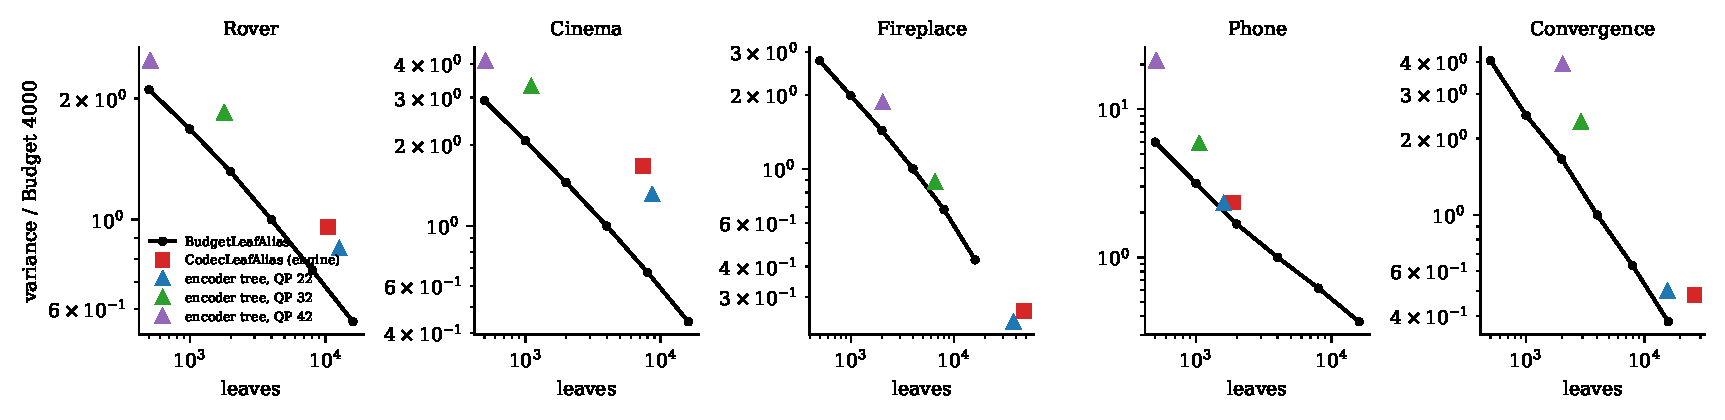
\includegraphics[width=\columnwidth]{fig_variance_vs_leaves.pdf}
  \caption{\newmat Light-sampling variance against leaf count, relative to BudgetLeafAlias with 4000 leaves (median over frames). Each line is BudgetLeafAlias from 500 to 16000 leaves in one scene, and the square of the same color is the CodecLeafAlias partition of that scene. }
  \label{fig:variance}
\end{figure}

A codec partition fails in two situations. On dark or low-contrast content the leaves go to dark detail: the Cinema partition has 7400 leaves and still 1.67 times the variance of 4000 budget leaves. And the leaf count swings with the content, by 40 times within the Phone video (528 to 20133), and with it the memory (0.2 to 2.2\,MB per frame) and the sampling cost, against a fixed 75\,KB. In summary, CodecLeafAlias is preferable when a decoded stream is at hand, the light is concentrated or the content bright and detailed, and a variable memory footprint is acceptable. BudgetLeafAlias is preferable when memory or cache size must be bounded, on dark or fading content, whenever predictable cost matters, and for emissive textures that are not decoded from a stream at all (rendered, procedural or uncompressed). The two can be combined by merging a codec partition down to a budget with the same $\mathrm{Var}\cdot A$ rule. 

\paragraph{Quantization and bitrate.}
As discussed in Section~\ref{sec:codec}, compression does not introduce bias to the estimate, so the question is how much variance it adds. We encoded the five videos in 10-bit PQ with libvpx-vp9 (CRF 12, 32, 48, 63), x265 (CRF 18, 28, 40) and SVT-AV1 (CRF 25, 40, 55), from 74 down to 0.6\,Mb/s (decoded PSNR from 51 to 32\,dB), took the leaf weights from the decoded planes as described in Section~\ref{sec:codec}, and rendered one inter-coded frame per scene at equal samples (32 captures) against the same partition with exact leaf weights.

Every ratio lies between 0.995 and 1.029 (Figure~\ref{fig:rate}), the largest PSNR loss is 0.23\,dB, and the ratios do not grow as the bitrate falls: compression error is spread over each block, while a leaf weight is the mean over the whole leaf, so most of it averages out. Taking the partition from the decoded frame instead of the source gives 0.996--1.019. Quantizing the block means directly isolates the effect of the DC quantizer: up to a step of 64 of the 1023 code values the error grows by about 3\% at most, for both partitions, and only a step of 256, a quarter of the range, reaches 4--13\%. Using the luma mean alone instead of the three planes changes the error by at most 1.5\%. 

\begin{figure}[htbp!]
  \centering
  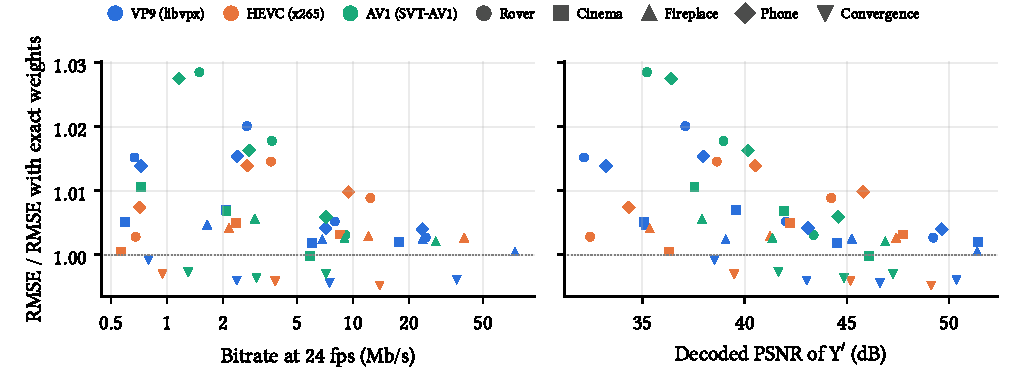
\includegraphics[width=\columnwidth]{fig_rate_sensitivity.pdf}
  \caption{\newmat RMSE of the rendered frame with leaf weights taken from lossy encodes, relative to exact leaf weights, against bitrate (left) and decoded PSNR (right), for three codecs and five scenes. All 50 points lie between 0.995 and 1.029, with no trend toward low bitrates.}
  \label{fig:rate}
\end{figure}

\paragraph{Other codecs and encoder settings.}
CodecLeafAlias needs two things from a codec: a block partition that follows image content, and the mean of each block. Every block-based codec provides the second; the first depends on the frame type. A standard configuration chooses blocks by rate-distortion (RD) search. In an intra-coded frame this splits where the image is detailed, which is what the sampler needs. In a predicted frame the search runs on the residual left after motion compensation, so its blocks follow prediction error rather than content: where motion is predicted well, a detailed region can be coded as one large block (Figure~\ref{fig:trees}).

\begin{figure}[htbp!]
  \centering
  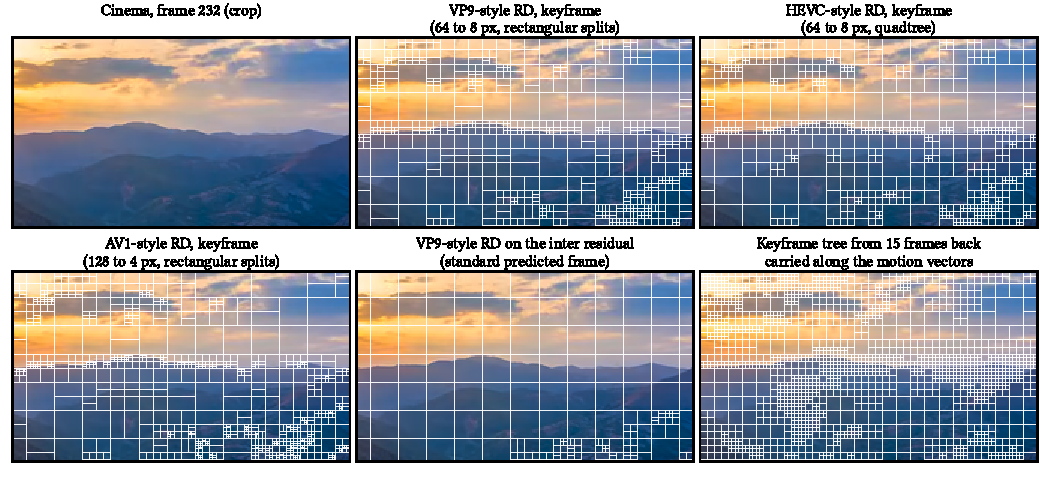
\includegraphics[width=\columnwidth]{fig_codec_trees.pdf}
  \caption{\newmat Partitions of a Cinema frame at quantizer 64 of 1023. Keyframe RD trees of the three codec families follow content. The RD tree of a predicted frame (bottom middle) follows prediction error instead and leaves most of the details in large blocks. The keyframe tree carried along the motion vectors (bottom right) follows content again.}
  \label{fig:trees}
\end{figure}

We reproduced the partition search of the three codec families on our frames, with their block sizes and split modes (VP9 and HEVC from 64 to 8 pixels, AV1 from 128 to 4), at quantizers 16, 64 and 256 of 1023, and rendered each partition with exact leaf means at equal samples. Used directly, the RD tree of a predicted frame costs up to 12\% for VP9 and HEVC and 22\% for AV1 at quantizer 64, relative to the CodecLeafAlias partition. Reusing the last keyframe's tree without moving it is better but drifts as the content moves (up to 6\%). Carrying the keyframe tree along the motion vectors of the stream, the strategy proposed in Section~\ref{sec:codec}, solves both: it stays within 2.5--4.2\% of the CodecLeafAlias partition at quantizers 16 and 64 for all three codec families, and within 5.4--6.6\% at quantizer 256, which is comparable to a partition built without any codec data. The three families behave alike for every partition source, and with weights from real encodes their worst ratios are 1.020 (VP9), 1.015 (HEVC) and 1.029 (AV1). The method is therefore tied neither to VP9 nor to its variance partitioning mode. 
\newend

\subsection{Denoised Results}
\label{sec:denoise}
Real-time renders are frequently paired with a neural denoiser in production. We pass each
technique's calibrated real-time render through the same OptiX denoiser~\cite{nvidia2021optixdenoiser} and re-measure
RMSE against the reference. Table~\ref{tab:denoise} shows that on every scene tested,
starting from our lower-noise image lets the denoiser reach a lower final RMSE than starting
from Random or 2D CDF.

\begin{table}[htbp!]
\centering
\small
\caption{RMSE before and after denoising. On every scene tested, whichever of our two techniques wins that scene keeps the lowest denoised RMSE too. }
\label{tab:denoise}
\begin{tabular}{ll cc}
\toprule
Scene & Technique & Noisy RMSE & Denoised RMSE \\
\midrule
\multirow{3}{*}{Rover}
 & Random & 0.0468 & 0.0381 \\
 & 2D CDF & 0.0779 & 0.0424 \\
 & {BudgetLeafAlias} & \textbf{0.0367} & \textbf{0.0375} \\
\midrule
\multirow{3}{*}{Cinema}
 & Random & 0.1109 & 0.0111 \\
 & 2D CDF & 0.1218 & 0.0110 \\
 & {CodecLeafAlias} & \textbf{0.0933} & \textbf{0.0106} \\
\midrule
\multirow{3}{*}{Fireplace Room}
 & Random & 0.5516 & 0.0312 \\
 & 2D CDF & 0.2295 & 0.0233 \\
 & {CodecLeafAlias} & \textbf{0.2087} & \textbf{0.0225} \\
\midrule
\multirow{3}{*}{Convergence}
 & Random & 0.3296 & 0.0148 \\
 & 2D CDF & 0.1428 & 0.0041 \\
 & {CodecLeafAlias} & \textbf{0.0870} & \textbf{0.0034} \\
\bottomrule
\end{tabular}
\end{table}


Convergence benefits the most: denoising cuts RMSE by over $95\,\%$ for every technique, and
CodecLeafAlias still finishes with the lowest denoised RMSE of the three ($0.0034$,
against $0.0041$ for 2D CDF), a direct result of feeding the denoiser a cleaner starting
image. Figure~\ref{fig:denoisedflip} additionally shows
denoised closeups and their \FLIP\  error maps for Convergence and Fireplace Room. 2D CDF's denoised output keeps a visibly brighter (higher-error) \FLIP\ map.

\new{The differences between techniques are nevertheless much smaller after denoising than before it, for two reasons. First, the denoiser removes mostly the high-frequency, per-pixel part of the error, which is precisely where light samplers differ; what remains is dominated by low-frequency residue that depends little on the number of light samples. Second, as discussed in Section~\ref{sec:equalquality}, light sampling is only one term of the error of a frame, so the room for any emission sampler is bounded before the denoiser acts. For a denoised pipeline the practical reading is the one of Section~\ref{sec:equalquality}: similar final quality is obtained from a sampler that costs less time and memory.}

Figure~\ref{fig:teaser} shows full-frame comparisons and closeups for Rover and Cinema, where
BudgetLeafAlias and CodecLeafAlias respectively remove most of the speckled noise still
visible in Random and 2D CDF's closeups. Figure~\ref{fig:figuresonly} shows
the same treatment for the remaining three scenes against a converged reference, with two matched closeups per scene; each panel also shows, in its top-left
corner, the actual HDR emissive texture that lit that scene. CodecLeafAlias visibly reduces
noise relative to both baselines.

\begin{figure*}[htbp!]
  \centering
  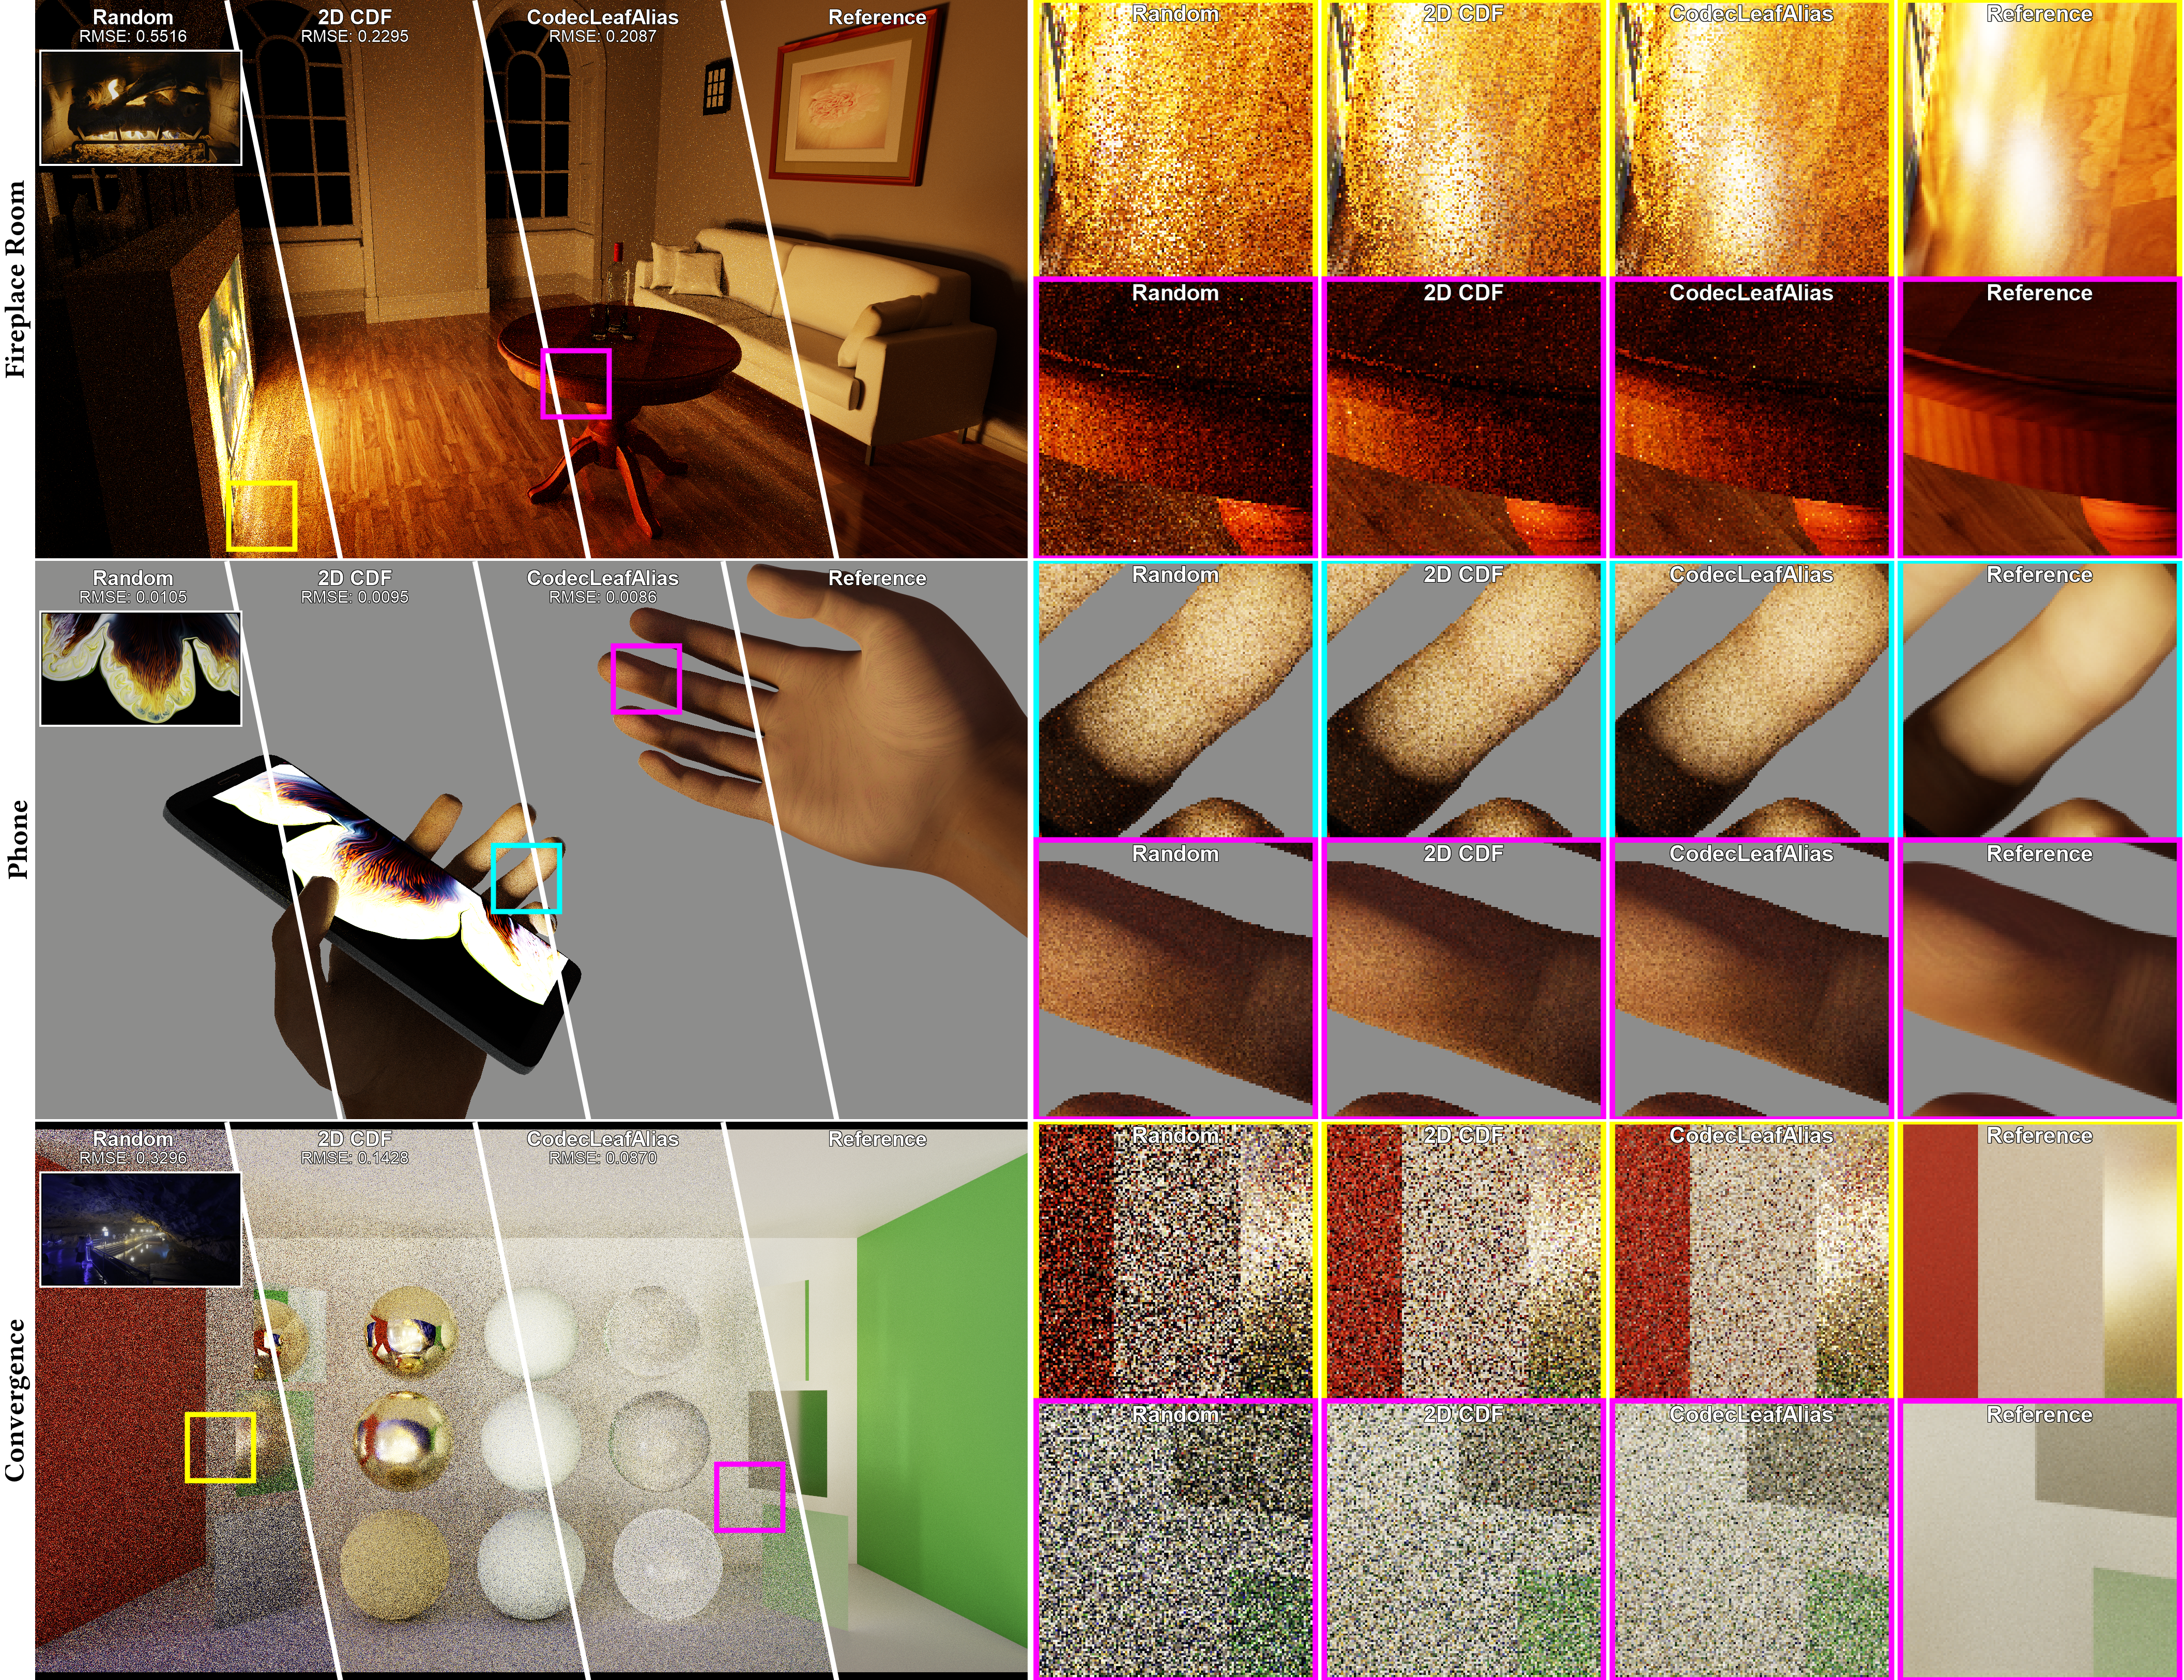
\includegraphics[width=\textwidth]{figures_only_restir_v9.png}
  \caption{Fireplace Room, Phone, and Convergence: full-frame diagonal comparisons
  (Random / 2D CDF / CodecLeafAlias / Reference) with real measured RMSE per technique, two
  large matched closeups per scene, and each scene's emissive HDR texture (top-left inset). }
  \label{fig:figuresonly}
\end{figure*}

\begin{figure*}[htbp!]
  \centering
  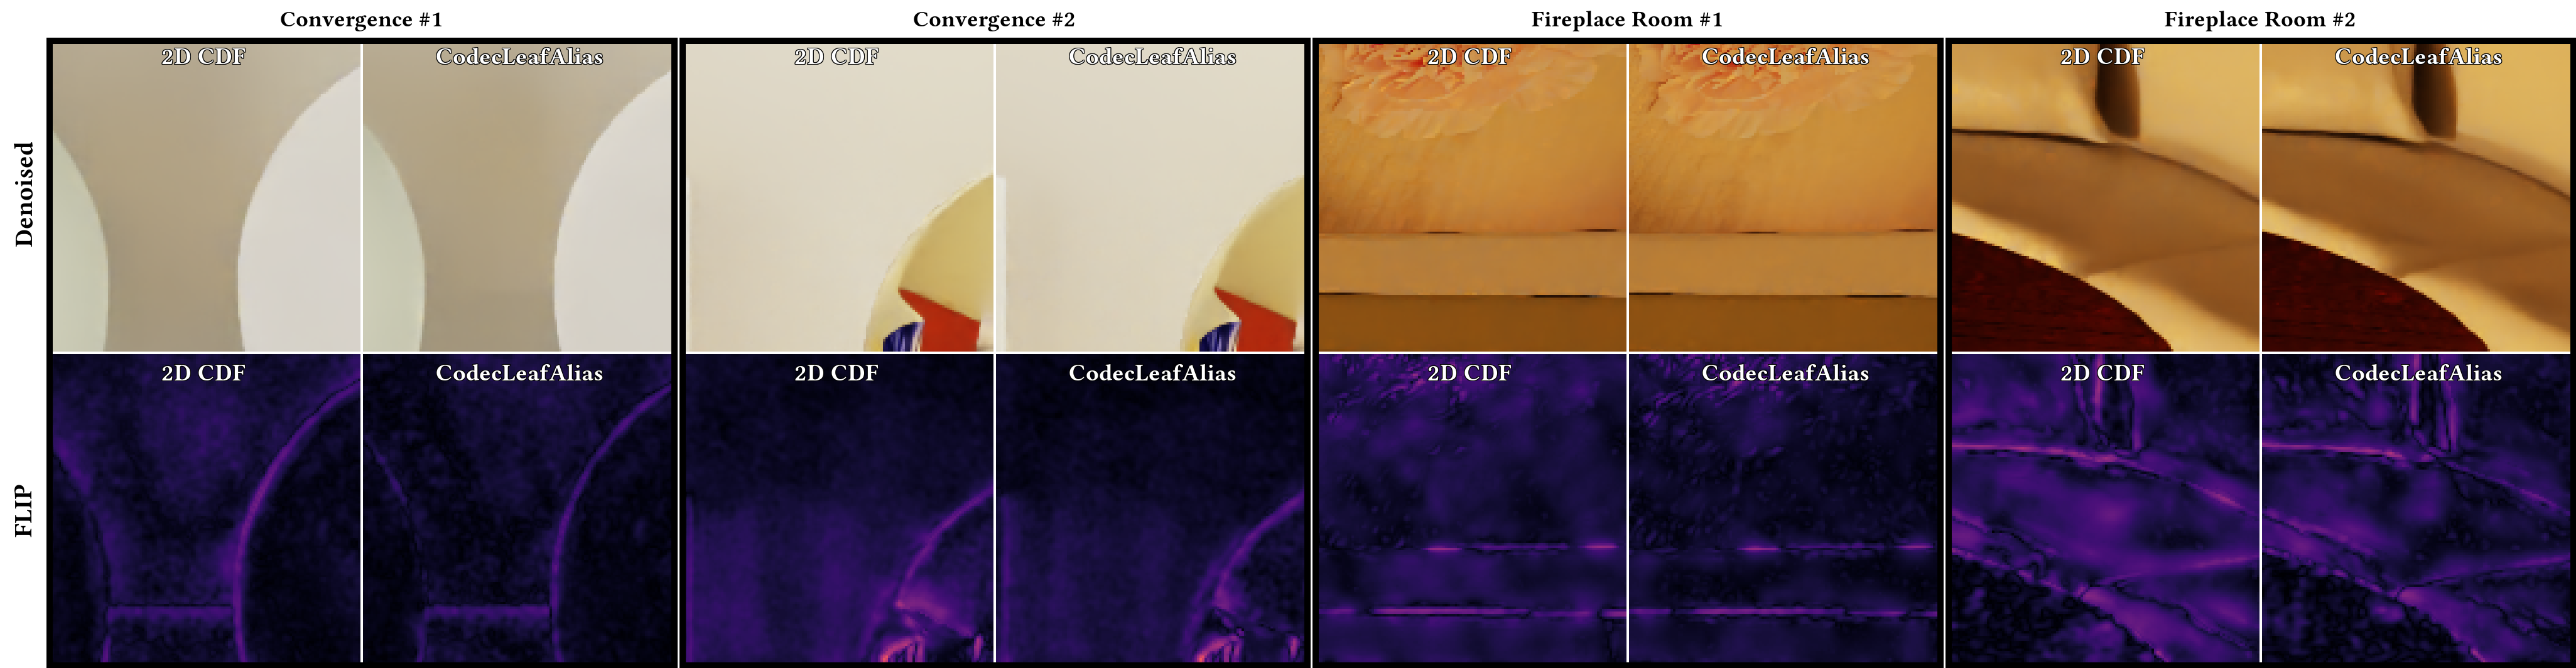
\includegraphics[width=\textwidth]{denoised_flip_grid.png}
  \caption{Denoised closeups and FLIP error maps when compared to the reference, for 2D CDF
  and CodecLeafAlias, at the two regions per scene with the largest denoised FLIP gap, for
  Convergence and Fireplace Room.}
  \label{fig:denoisedflip}
\end{figure*}

\subsection{\texorpdfstring{\newt{Discussion and limitations}}{Discussion and limitations}}
\label{sec:limits}

\newbegin
LeafAlias helps most when the sampling structure has to be small and cheap: several video lights at once, high-resolution emitters, limited memory or upload bandwidth, a tight frame, and scenes where the light sampler accounts for a large part of the error. Its limits follow from the same measurements. (i)~At equal samples it is never better than a per-texel distribution; a larger leaf budget reduces the loss. (ii)~Its gain comes from fitting more light samples in the frame, so it disappears when light sampling is a small part of the frame's cost or of its error. (iii)~It considers the texture alone: the BSDF, visibility and the distance to the emitter contribute variance that no scene-independent emission sampler removes, which bounds the gain of any such sampler. (iv)~The alias mapping does not exploit low-discrepancy sample sequences (Appendix~\ref{app:qmc}); a monotone mapping such as a 2D CDF does. (v)~Our implementation stores the mean luminance of a leaf as a 16-bit float, which saturates at 65504; emitters with brighter texels may need a wider format. (vi)~Extracting the partitions from the encoded metadata might pose some difficulty in video workflows involving hardware-accelerated decoding pipelines..
\newend

\section{Conclusions and future work} \label{sec:conclusions}

We introduced LeafAlias, a family of samplers for dynamic emissive textures that build a per-frame alias table over a variance-driven quadtree rather than over raw pixels. \rev{The outcome is a sampler that is inexpensive enough to rebuild in every frame, small enough to stay resident in the GPU's L1 cache, and accurate enough to stay within a few percent of the per-texel methods we compared against at equal samples, while reaching their quality up to 3 times faster.}

\rev{The consistency of CodecLeafAlias results through the different video light sources, codecs and bitrates that were tested suggests that the coded signal carries enough information to be reused for importance sampling. The advantage holds up when quality is judged over a full animated sequence rather than a single frame, and narrows, as for any light sampler, once a denoiser is added to the pipeline.} We also show that, when not available, building a small variance-driven quadtree is fast and can improve performance. The decision to use more or fewer leaves depends on the scene complexity and video material.

More broadly, this work points to an under-exploited overlap between the toolchains of video compression and real-time rendering. We think this connection has more to offer than the single, frame-local piece of it used here. The most direct extension is temporal. The coding-tree partition is currently extracted in every frame, discarding the motion vectors the same encoder already computes to relate consecutive frames. Since those vectors describe how the variance structure itself is moving, they could warp the previous frame's leaves into a predicted partition for the current one.
A second direction targets the leaf weights rather than the partition. CodecLeafAlias currently estimates each leaf's radiance from a single DC coefficient, which is exact under a piecewise-constant model but discards the higher-frequency information. That information could be used to guide the sampling within the leaf rectangle, potentially improving the efficiency of each drawn sample. \new{A third is the mapping itself: a hierarchical warp~\cite{clarberg2005wavelet} down the same quadtree keeps the leaf density and its small footprint, and could recover the benefit of low-discrepancy sequences that the alias mapping gives up (Appendix~\ref{app:qmc}).}

Finally, because every LeafAlias sample already carries an unbiased pdf, it composes naturally with spatiotemporal resampling: using it purely as the candidate generator inside a ReSTIR-style reservoir, rather than as the final sampler, may provide additional variance reduction on scenes with several bright, moving regions competing for the light budget.

\bibliographystyle{ACM-Reference-Format}
\bibliography{sample-base}

\appendix

\section{\texorpdfstring{\newt{Per-pixel alias tables and low-discrepancy input}}{Per-pixel alias tables and low-discrepancy input}}
\label{app:qmc}

\newbegin
The results of the paper use independent random numbers. Renderers driven by quasi-Monte Carlo (QMC) sequences expose a further difference between a per-pixel alias table and a table over leaves, which we document here. The claim is limited: LeafAlias does \emph{not} exploit low-discrepancy input; it avoids a failure of per-pixel alias tables under such input. Since the Fourier spectrum of a non-uniform sample set is not a measure of its discrepancy under the target density~\cite{li2026gradient}, we do not rely on spectra, and measure the integration error of rendered images instead.

\paragraph{How the pattern arises.}
A per-pixel alias table maps a sample $(u,v)$ to bucket $k=\lfloor un\rfloor$ of $n$ (one per texel), keeps the bucket's own texel if $v<\tau_k$ and otherwise jumps to its alias. The $N$ values of $u$ that a pixel draws from a low-discrepancy sequence are spread almost evenly over $[0,1)$, so they visit the table at a nearly constant stride of $n/N$ buckets. Vose's construction, as implemented in our renderer, lists below-mean and above-mean texels in scan order and pairs them in that order, so inside any region whose texels are all on the same side of the mean (a smooth sky, a dark hillside) consecutive buckets own consecutive texels. The constant stride through the table becomes a constant stride through the image, $H/N$ rows for an image of height $H$: when $N$ divides $H$, every sample of a pixel that falls in such a region lands in the same column. Figure~\ref{fig:qmcpoints} shows it on a $1024{\times}512$ region of the Cinema texture: the 2D CDF keeps the even spread of the Halton input, while the per-pixel alias table stacks the samples of the hillside into lines. In the spectrum of 60000 points, the strongest line is 41 times its median for the per-pixel alias table, against 1.4 for the 2D CDF and for BudgetLeafAlias. Two conditions must hold together: a stride aligned with the image rows, and long scan-order runs in the table. A textbook construction that keeps scan order everywhere, as in Figure~\ref{fig:spectrum}, produces a lattice over the whole image. Owen-scrambled sequences~\cite{owen1995randomly} randomize the stride and, in our test, remove most of the effect.

\begin{figure}[htbp!]
  \centering
  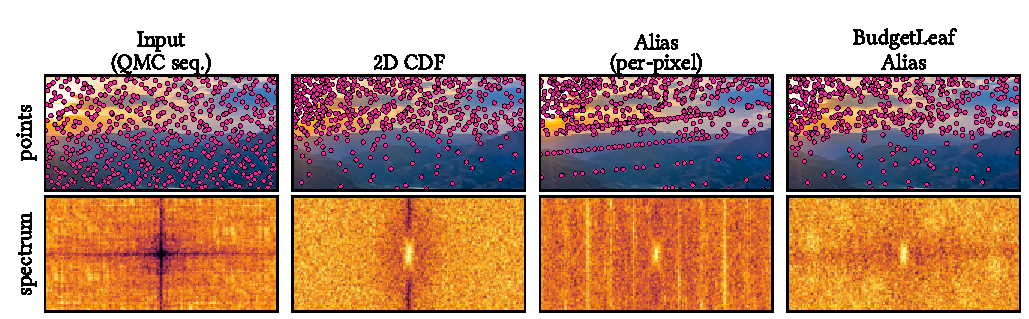
\includegraphics[width=\columnwidth]{fig_qmc_points.pdf}
  \caption{\newmat Top: the first 500 points of the Halton sequence (bases 2, 3), as input and after each warp, over a $1024{\times}512$ region of the Cinema texture. Bottom: power spectrum of the first 60000 points. The per-pixel alias table uses the table construction of our renderer; BudgetLeafAlias uses 4000 leaves.}
  \label{fig:qmcpoints}
\end{figure}

\paragraph{What it costs in a rendering.}
We render a diffuse floor lit by the textured area light through a fence (direct lighting, light sampling only, no MIS), with the Halton set and an independent toroidal shift per pixel, against an exact reference obtained by quadrature over the emitter (Figure~\ref{fig:qmcfence}, Table~\ref{tab:qmc}). With pseudorandom numbers the samplers are equal, as their densities predict. With QMC input the 2D CDF becomes 3.5 times better and the per-pixel alias table 2.6 times \emph{worse}, while LeafAlias stays at its pseudorandom level. The per-pixel alias table with QMC does not converge at all between 128 and 512 samples per pixel, where the stride is 4, 2 and 1 rows (relative RMSE 0.145 and 0.143 on the unoccluded part of the floor, against 0.054 and 0.025 for LeafAlias and 0.013 and 0.004 for the 2D CDF), and starts to fall only at 1024 samples.

\begin{figure}[htbp!]
  \centering
  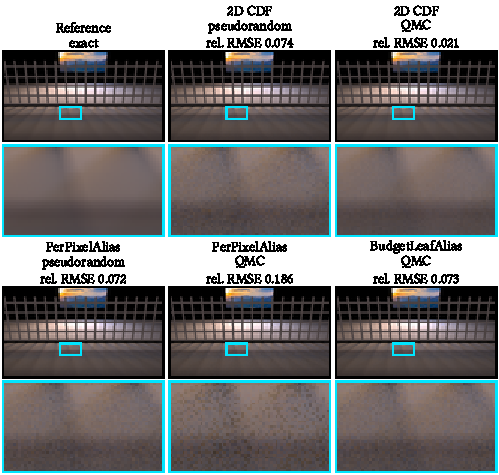
\includegraphics[width=0.92\columnwidth]{fig_qmc_fence.pdf}
  \caption{\newmat A diffuse floor lit through a fence by the emitter of Figure~\ref{fig:qmcpoints}, at 128 samples per pixel: exact reference; 2D CDF with pseudorandom and QMC input; per-pixel alias table with pseudorandom and QMC input; BudgetLeafAlias with QMC input. Close-ups below each render.}
  \label{fig:qmcfence}
\end{figure}

\begin{table}[htbp!]
\centering\small\newmat
\caption{\newmat Top: relative RMSE of the scene of Figure~\ref{fig:qmcfence} at 128 samples per pixel. Bottom: ratio of the QMC error to the sampler's own pseudorandom error over 2406 emitters and emitter regions (photographs, video frames, sky images and windows of our textures), one shading point behind six kinds of occluder.}
\label{tab:qmc}
\begin{tabular}{lcc}
\toprule
Relative RMSE, 128 spp & Pseudorandom & QMC \\
\midrule
2D CDF & 0.074 & 0.021 \\
Per-pixel Alias & 0.072 & 0.186 \\
BudgetLeafAlias (4000 leaves) & 0.074 & 0.073 \\
LeafAlias (1000 leaves) & 0.075 & 0.072 \\
\midrule
QMC error / own pseudorandom & 128 spp & 1024 spp \\
\midrule
Per-pixel Alias, median & 0.92 & 0.79 \\
\quad cases above 1.10 & 16.7\% & 7.3\% \\
\quad worst case & 1.85 & 3.51 \\
BudgetLeafAlias, median & 0.99 & 0.93 \\
\quad cases above 1.10 & 0.0\% & 0.5\% \\
\quad worst case & 1.10 & 1.20 \\
\bottomrule
\end{tabular}
\end{table}

This is not a property of one region: of 225 overlapping $1024{\times}512$ windows of the same frame, the per-pixel alias table with QMC is worse than with pseudorandom numbers in 131, and it is worse in 65\% of the 40 flat sky photographs we tested. Over 2406 emitters (Table~\ref{tab:qmc}, bottom), the QMC error of BudgetLeafAlias stays within 10\% of its own pseudorandom error in more than 99\% of the cases, whereas the per-pixel alias table exceeds that bound in 7--17\% of the cases and reaches 3.5 times. These magnitudes are a best case for QMC, a single two-dimensional direct-lighting integral; in a full path tracer both the gain of the 2D CDF and the loss of the per-pixel alias table are smaller.

\paragraph{Scope.}
A table over a few thousand leaves, each covering many texels, has no fixed relation between bucket stride and image position, so it creates no pattern; but it does not preserve the low-discrepancy distribution either, and its QMC and pseudorandom errors are the same. The 2D CDF and hierarchical warps do preserve it, at the memory and per-sample cost reported in Section~\ref{sec:cost}, and the 2D CDF remains the lowest-error sampler under QMC when that cost is not a concern. On emitters that do not trigger the pattern, among them the five videos of this paper, the per-pixel alias table with QMC input had lower error than LeafAlias. The advantage of LeafAlias here is predictability: its error does not depend on whether the pattern conditions are met. The \supp{qmc\_note}, with its code, reproduces these figures and tables and adds a convergence study.
\newend

\section{\texorpdfstring{\newt{Temporal stability}}{Temporal stability}}
\label{app:temporal}

\newbegin
We evaluate temporal stability on 60 consecutive frames of each scene, rendered at equal samples with a new random seed every frame, against a converged reference for every frame. With $I_t$ the render and $R_t$ the reference of frame $t$, the \emph{temporal error} is
\begin{equation}
E_T = \sqrt{\left\langle\left[(I_t - I_{t-1}) - (R_t - R_{t-1})\right]^2\right\rangle},
\end{equation}
averaged over pixels and frames: subtracting the reference's own change removes what the video itself does, so only change introduced by the renderer remains. The \emph{low-frequency temporal error} is the same quantity after a Gaussian blur with $\sigma = 8$ pixels, which averages out per-pixel noise and keeps the kind of change that is seen as flicker, regions pulsing or popping between frames. Independently of rendering, we measure how much the sampling density changes between consecutive frames with the Jensen--Shannon divergence.

\paragraph{The coarser density changes less.} A per-texel density follows every change of the video, including compression noise, grain and small moving details. A leaf density averages each region over many texels, so these small changes largely cancel, and a leaf boundary that moves between frames only reassigns probability between neighbouring leaves of similar radiance. The density of BudgetLeafAlias changes 5.4, 2.5, 2.5 and 1.8 times less than the exact one in Rover, Cinema, Phone and Convergence, and about the same in Fireplace Room (Figure~\ref{fig:temporal}, left), even though 3--13\% of the $8{\times}8$ cells change leaf size every frame.

\begin{figure}[t]
  \centering
  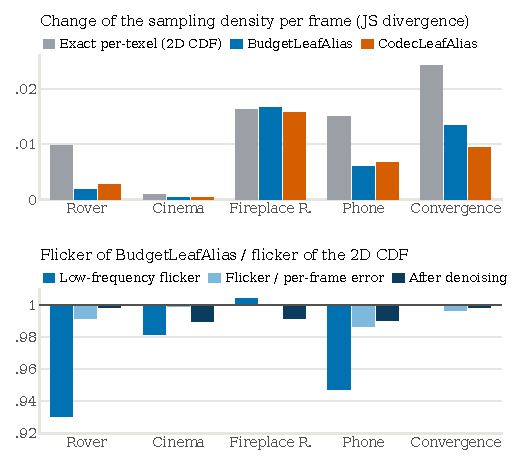
\includegraphics[width=\columnwidth]{fig_temporal.pdf}
  \caption{\newmat Top: change of the sampling density between consecutive frames, for the exact per-texel density (the 2D CDF's) and for the two LeafAlias densities. Bottom: rendered flicker of BudgetLeafAlias divided by the 2D CDF's, at equal samples; below 1 means less flicker.}
  \label{fig:temporal}
\end{figure}

\paragraph{Rendered flicker.} The low-frequency temporal error of BudgetLeafAlias is lower than the 2D CDF's in Rover, Cinema and Phone (7\%, 2\% and 5\% less) and the same in Fireplace Room and Convergence; that of CodecLeafAlias is within 0.0002 of the 2D CDF's in every scene (values of 0.0026--0.0072). The standard deviation over frames of the mean error of the whole frame (brightness pumping) is the same for all techniques. The full temporal error includes the per-pixel noise of each frame, so it grows with the per-frame error: BudgetLeafAlias is equal to or below the 2D CDF in Rover, Cinema and Phone and 4\% above it in Fireplace Room and Convergence, the two scenes where its per-frame RMSE is also 4--5\% higher. Divided by the per-frame RMSE, its temporal error is lower than the 2D CDF's in all five scenes: the partition changes add nothing measurable beyond the per-frame noise. After the OptiX denoiser, the temporal error of BudgetLeafAlias is equal to or lower than the 2D CDF's in every scene (Figure~\ref{fig:temporal}, right).

\paragraph{Frozen noise.} As a diagnostic, we also froze the random numbers (same seed every frame, no camera jitter), so that the image changes only through the video and the sampling structure. In that setting, where noise no longer hides it, the changing partition is visible as a fine-grained per-pixel change 1.5--3.6 times larger than the 2D CDF's, and a hierarchical warp over the same leaves brings it to 1.03--1.32 times. This setting does not occur in normal rendering, where a new seed every frame makes this change part of the per-frame noise, but it matters for techniques that reuse random numbers across frames, which we did not evaluate. The \supp{temporal\_stability} contains the complete tables.
\newend

\end{document}
